% Options for packages loaded elsewhere
% Options for packages loaded elsewhere
\PassOptionsToPackage{unicode}{hyperref}
\PassOptionsToPackage{hyphens}{url}
\PassOptionsToPackage{dvipsnames,svgnames,x11names}{xcolor}
%
\documentclass[
  12pt,
  letterpaper,
  DIV=11,
  numbers=noendperiod]{scrreprt}
\usepackage{xcolor}
\usepackage[margin=1in]{geometry}
\usepackage{amsmath,amssymb}
\setcounter{secnumdepth}{5}
\usepackage{iftex}
\ifPDFTeX
  \usepackage[T1]{fontenc}
  \usepackage[utf8]{inputenc}
  \usepackage{textcomp} % provide euro and other symbols
\else % if luatex or xetex
  \usepackage{unicode-math} % this also loads fontspec
  \defaultfontfeatures{Scale=MatchLowercase}
  \defaultfontfeatures[\rmfamily]{Ligatures=TeX,Scale=1}
\fi
\usepackage{lmodern}
\ifPDFTeX\else
  % xetex/luatex font selection
\fi
% Use upquote if available, for straight quotes in verbatim environments
\IfFileExists{upquote.sty}{\usepackage{upquote}}{}
\IfFileExists{microtype.sty}{% use microtype if available
  \usepackage[]{microtype}
  \UseMicrotypeSet[protrusion]{basicmath} % disable protrusion for tt fonts
}{}
\makeatletter
\@ifundefined{KOMAClassName}{% if non-KOMA class
  \IfFileExists{parskip.sty}{%
    \usepackage{parskip}
  }{% else
    \setlength{\parindent}{0pt}
    \setlength{\parskip}{6pt plus 2pt minus 1pt}}
}{% if KOMA class
  \KOMAoptions{parskip=half}}
\makeatother
% Make \paragraph and \subparagraph free-standing
\makeatletter
\ifx\paragraph\undefined\else
  \let\oldparagraph\paragraph
  \renewcommand{\paragraph}{
    \@ifstar
      \xxxParagraphStar
      \xxxParagraphNoStar
  }
  \newcommand{\xxxParagraphStar}[1]{\oldparagraph*{#1}\mbox{}}
  \newcommand{\xxxParagraphNoStar}[1]{\oldparagraph{#1}\mbox{}}
\fi
\ifx\subparagraph\undefined\else
  \let\oldsubparagraph\subparagraph
  \renewcommand{\subparagraph}{
    \@ifstar
      \xxxSubParagraphStar
      \xxxSubParagraphNoStar
  }
  \newcommand{\xxxSubParagraphStar}[1]{\oldsubparagraph*{#1}\mbox{}}
  \newcommand{\xxxSubParagraphNoStar}[1]{\oldsubparagraph{#1}\mbox{}}
\fi
\makeatother
\usepackage{listings}
\newcommand{\passthrough}[1]{#1}
\lstset{defaultdialect=[5.3]Lua}
\lstset{defaultdialect=[x86masm]Assembler}


\usepackage{longtable,booktabs,array}
\usepackage{calc} % for calculating minipage widths
% Correct order of tables after \paragraph or \subparagraph
\usepackage{etoolbox}
\makeatletter
\patchcmd\longtable{\par}{\if@noskipsec\mbox{}\fi\par}{}{}
\makeatother
% Allow footnotes in longtable head/foot
\IfFileExists{footnotehyper.sty}{\usepackage{footnotehyper}}{\usepackage{footnote}}
\makesavenoteenv{longtable}
\usepackage{graphicx}
\makeatletter
\newsavebox\pandoc@box
\newcommand*\pandocbounded[1]{% scales image to fit in text height/width
  \sbox\pandoc@box{#1}%
  \Gscale@div\@tempa{\textheight}{\dimexpr\ht\pandoc@box+\dp\pandoc@box\relax}%
  \Gscale@div\@tempb{\linewidth}{\wd\pandoc@box}%
  \ifdim\@tempb\p@<\@tempa\p@\let\@tempa\@tempb\fi% select the smaller of both
  \ifdim\@tempa\p@<\p@\scalebox{\@tempa}{\usebox\pandoc@box}%
  \else\usebox{\pandoc@box}%
  \fi%
}
% Set default figure placement to htbp
\def\fps@figure{htbp}
\makeatother





\setlength{\emergencystretch}{3em} % prevent overfull lines

\providecommand{\tightlist}{%
  \setlength{\itemsep}{0pt}\setlength{\parskip}{0pt}}



 


% header.tex
\usepackage{fvextra}
\usepackage{etoolbox}
\usepackage{enumitem}
\usepackage{inconsolata}
\renewcommand{\partname}{Module}
\usepackage{float}
\renewcommand*{\partformat}{\partname~\thepart\autodot}
\usepackage[T1]{fontenc}        % <-- add this
\usepackage{textcomp}           % good companion to T1 (optional but helpful)
\usepackage[scaled=0.95]{helvet}
\renewcommand{\familydefault}{\sfdefault}
\providecommand{\FunctionTok}[1]{#1}
\renewcommand{\FunctionTok}[1]{#1}
% 1) Make Pandoc/Quarto code blocks NOT wrap
%    (Pandoc uses a Verbatim-based env called "Highlighting")
\DefineVerbatimEnvironment{Highlighting}{Verbatim}{
  commandchars=\\\{\},
  breaklines=false,
  breakanywhere=false,
  fontsize=\footnotesize
}

% 2) Output blocks are typically inside a "Shaded" environment
%    (make them smaller too)
\AtBeginEnvironment{Shaded}{\footnotesize}

% 3) Extra safety: tell fancyvrb/fvextra never to break lines
\fvset{breaklines=false, breakanywhere=false}
\usepackage{booktabs}
\usepackage{longtable}
\usepackage{array}
\usepackage{multirow}
\usepackage{wrapfig}
\usepackage{float}
\usepackage{colortbl}
\usepackage{pdflscape}
\usepackage{tabu}
\usepackage{threeparttable}
\usepackage{threeparttablex}
\usepackage[normalem]{ulem}
\usepackage{makecell}
\usepackage{xcolor}
\KOMAoption{captions}{tableheading}
\makeatletter
\@ifpackageloaded{tcolorbox}{}{\usepackage[skins,breakable]{tcolorbox}}
\@ifpackageloaded{fontawesome5}{}{\usepackage{fontawesome5}}
\definecolor{quarto-callout-color}{HTML}{909090}
\definecolor{quarto-callout-note-color}{HTML}{0758E5}
\definecolor{quarto-callout-important-color}{HTML}{CC1914}
\definecolor{quarto-callout-warning-color}{HTML}{EB9113}
\definecolor{quarto-callout-tip-color}{HTML}{00A047}
\definecolor{quarto-callout-caution-color}{HTML}{FC5300}
\definecolor{quarto-callout-color-frame}{HTML}{acacac}
\definecolor{quarto-callout-note-color-frame}{HTML}{4582ec}
\definecolor{quarto-callout-important-color-frame}{HTML}{d9534f}
\definecolor{quarto-callout-warning-color-frame}{HTML}{f0ad4e}
\definecolor{quarto-callout-tip-color-frame}{HTML}{02b875}
\definecolor{quarto-callout-caution-color-frame}{HTML}{fd7e14}
\makeatother
\makeatletter
\@ifpackageloaded{bookmark}{}{\usepackage{bookmark}}
\makeatother
\makeatletter
\@ifpackageloaded{caption}{}{\usepackage{caption}}
\AtBeginDocument{%
\ifdefined\contentsname
  \renewcommand*\contentsname{Table of contents}
\else
  \newcommand\contentsname{Table of contents}
\fi
\ifdefined\listfigurename
  \renewcommand*\listfigurename{List of Figures}
\else
  \newcommand\listfigurename{List of Figures}
\fi
\ifdefined\listtablename
  \renewcommand*\listtablename{List of Tables}
\else
  \newcommand\listtablename{List of Tables}
\fi
\ifdefined\figurename
  \renewcommand*\figurename{Figure}
\else
  \newcommand\figurename{Figure}
\fi
\ifdefined\tablename
  \renewcommand*\tablename{Table}
\else
  \newcommand\tablename{Table}
\fi
}
\newcommand*\listoflistings\lstlistoflistings
\AtBeginDocument{%
\renewcommand*\lstlistlistingname{List of Listings}
}
\makeatother
\makeatletter
\makeatother
\makeatletter
\@ifpackageloaded{caption}{}{\usepackage{caption}}
\@ifpackageloaded{subcaption}{}{\usepackage{subcaption}}
\makeatother
\usepackage{bookmark}
\IfFileExists{xurl.sty}{\usepackage{xurl}}{} % add URL line breaks if available
\urlstyle{same}
\hypersetup{
  pdftitle={Introduction to Business Statistics: A Modeling Approach},
  pdfauthor={Viswa Viswanathan},
  colorlinks=true,
  linkcolor={blue},
  filecolor={Maroon},
  citecolor={Blue},
  urlcolor={Blue},
  pdfcreator={LaTeX via pandoc}}


\title{Introduction to Business Statistics: A Modeling Approach}
\author{Viswa Viswanathan}
\date{2026-01-15}
\begin{document}
\maketitle

\renewcommand*\contentsname{Table of contents}
{
\hypersetup{linkcolor=}
\setcounter{tocdepth}{2}
\tableofcontents
}

\bookmarksetup{startatroot}

\chapter*{Introduction to Business
Statistics}\label{introduction-to-business-statistics}
\addcontentsline{toc}{chapter}{Introduction to Business Statistics}

\markboth{Introduction to Business Statistics}{Introduction to Business
Statistics}

\emph{A Modeling and Regression-Based Approach}

Most business statistics courses start with probability.

This one starts with decisions.

Business leaders do not begin with sampling distributions --- they begin
with questions: What drives sales? What predicts customer churn? What
explains profitability?

To answer those questions, we build models.

This book takes a modeling-first approach. You will begin with data
visualization and variability, move to averages as models, then to
category means, and ultimately to regression models that explain and
predict business outcomes.

Only after you understand how models work do we introduce probability,
confidence intervals, and hypothesis testing --- as tools for
quantifying uncertainty in the models you build.

By the end of this book, you will be able to:

\begin{itemize}
\tightlist
\item
  explore and visualize data
\item
  understand variability
\item
  build and interpret regression models
\item
  evaluate how much variation a model explains
\item
  make data-driven decisions under uncertainty
\end{itemize}

Statistics is not about memorizing formulas. It is about building useful
models for real decisions.

Let's begin.

\bookmarksetup{startatroot}

\chapter*{Preface}\label{preface}
\addcontentsline{toc}{chapter}{Preface}

\markboth{Preface}{Preface}

This book accompanies the course \emph{Introduction to Business
Statistics (BQUA2811)} at Stillman School of Business. It takes
inspiration from \emph{Lessons in Statistical Thinking} by Daniel Kaplan
(\emph{LST}). \emph{LST} takes a modeling-centric approach and changes
the ordering of topics significantly from traditional introductory
statistics courses. \emph{LST} uses almost no mathematical notation, and
only provides intuitive explanation for most concepts -- which serves a
first statistics course for undergraduate business students very well.

After teaching the course for two semesters broadly using the \emph{LST}
approach, I found some need for changes. The following main drivers
shaped the changes:

\begin{itemize}
\tightlist
\item
  Students benefit from understanding structure before encountering
  uncertainty
\item
  A modeling-centric approach helps to provide an overarching course
  focus
\item
  Courses that depend on BQUA2811 primarily expect students to be
  competent in linear regression and related statistics concepts.
\end{itemize}

I wanted to provide more of a business focus and use more
business-related data sets than \emph{LST} does. More importantly, I
felt that \emph{LST} introduces \emph{statistical models} very
early.Even the very first plots -- lines and point estimates -- that
students encounter, show confidence bands. Despite emphasizing the
difference between \emph{mathematical models} and \emph{statistical
models} and providing many examples and illustrations from daily life, I
found that students had a very hard time understanding the idea of a
\emph{statistical model}.

I surmised that teaching the idea of models and concepts relating to
uncertainty together made it very challenging for students. Therefore I
decided to make a big change and restrict the initial discussion of
models to just the data set used for modeling without bringing up the
idea of inference from the model. Once students grasp the idea of a
least squares model independent of uncertainty, learn what it means to
\emph{explain} variation, and eventually grasp R-squared, we can then
layer on uncertainty that arises when we use a model in broader
contexts.

I also learned that even in developing the notion of a model, it is
pedagogically very useful to ramp it up gradually starting from mean as
the simplest model (when we have no explanatory variables), category
means as models when we have a categorical explanatory variable, and
finally extending to full-blown least-square models when the explanatory
variable is also numerical. Once students grasp the idea of model, it
then becomes easier to introduce uncertainty, probability and confidence
intervals.

Because of this change, I needed the initial plots to only plot lines
instead of confidence bands. However the plotting function from the
\emph{LSTbook} package that accompanies \emph{LST} only provides bands.
I therefore created a package named \emph{LSTextras} to extend the
functionality of \emph{LSTbook} package in a very small way to enable
plotting of point estimates and linear models without confidence bands.
I also included several business-related and data sets tuned for
illustrating specific concepts in the package. Combined with the data
sets already available in \emph{LSTbook} and the other packages like
\emph{ggplot2} that it depends on, students using \emph{LSTextras} will
have no dearth of data to experiment and explore the concepts that they
learn.

The book is organized into 14 modules reflecting this story line.

\part{Data, Visualization, and Patterns}

\chapter*{Module 1: Data, Visualization \&
Patterns}\label{module-1-data-visualization-patterns}
\addcontentsline{toc}{chapter}{Module 1: Data, Visualization \&
Patterns}

\markboth{Module 1: Data, Visualization \& Patterns}{Module 1: Data,
Visualization \& Patterns}

This module introduces the basic building blocks of statistical
thinking: data frames, variables, point plots and relationships. We
begin with visualization because patterns reveal what models will later
formalize.

\section*{Learning Goals}\label{learning-goals}
\addcontentsline{toc}{section}{Learning Goals}

\markright{Learning Goals}

\begin{itemize}
\tightlist
\item
  Describe data frames, variables, and instances\\
\item
  Perform simple manipulations of data frames using R
\item
  Create and interpret scatterplots using the \emph{point\_plot}
  function
\item
  Recognize patterns: direction, form, strength
\end{itemize}

\section*{Structure of This Module}\label{structure-of-this-module}
\addcontentsline{toc}{section}{Structure of This Module}

\markright{Structure of This Module}

\begin{itemize}
\tightlist
\item
  Data frames\\
\item
  Scatterplots
\item
  Relationships between variables
\end{itemize}

\chapter{Data Frames and Variables}\label{data-frames-and-variables}

We store data in an R object called a \emph{Data frame}. This chapter
introduces \textbf{data frames}, explains their key components and
teaches you how to get some basic information from them. We will learn
more in later chapters.

\section*{Learning outcomes}\label{learning-outcomes}
\addcontentsline{toc}{section}{Learning outcomes}

\markright{Learning outcomes}

\subsection*{After working though this chapter, you will be able
to:}\label{after-working-though-this-chapter-you-will-be-able-to}
\addcontentsline{toc}{subsection}{After working though this chapter, you
will be able to:}

\begin{itemize}
\tightlist
\item
  Explain the term \emph{data frame}
\item
  Explain what a column and row of a data frame represent
\item
  Name the two types of variables that we will deal with in this course
\item
  Distinguish between \emph{numerical} and \emph{categorical} variables
  and provide examples of each
\item
  Explain what the term \emph{level} of a categorical variable
  represents, and provide examples
\item
  Explain why a column is also called a \emph{variable}
\item
  Explain why a row is called an \emph{instance} or \emph{specimen}
\item
  Demonstrate the following skills related to R:

  \begin{itemize}
  \tightlist
  \item
    load a data frame from a loaded package
  \item
    explain what the \emph{pipe} operator does
  \item
    look at the first few rows in a data frame
  \item
    look at the last few rows in a data frame
  \item
    retrieve only the rows that satisfy certain conditions
  \item
    retrieve a subset of the columns of a data frame
  \item
    find the number of rows and columns in a data frame
  \item
    compute the average of a numeric column in a data frame
  \item
    use the \emph{count} function to compute the number of rows in a
    data frame for each level of a categorical variable
  \end{itemize}
\end{itemize}

\section{The R Software Package for
Statistics}\label{the-r-software-package-for-statistics}

In this course, we will be using the R software package for all
computations and visualizations. While R offers a great deal of
functionality, we will be using a limited subset that suffices for the
course topics. In particular, we will be using two specific R packages
that contain all the functions and data we need for the course. You
should install R and RStudio using the instructions provided in the
appendix. That section also shows you how to use RStudio and how to load
a package -- specifically the \emph{LSTbook} and \emph{LSTextras}
packages -- into R.

\section{R Data Frames}\label{r-data-frames}

In R, we generally represent data in a simple tabular structure named
\emph{data frame} -- a table with rows and columns.
Table~\ref{tbl-boston-marathon} shows an example of some initial rows
from the \emph{Boston\_marathon} data frame contained in the
\emph{LSTbook} package.

\begin{longtable}[]{@{}
  >{\raggedleft\arraybackslash}p{(\linewidth - 10\tabcolsep) * \real{0.0735}}
  >{\raggedright\arraybackslash}p{(\linewidth - 10\tabcolsep) * \real{0.3971}}
  >{\raggedright\arraybackslash}p{(\linewidth - 10\tabcolsep) * \real{0.2059}}
  >{\raggedright\arraybackslash}p{(\linewidth - 10\tabcolsep) * \real{0.1324}}
  >{\raggedright\arraybackslash}p{(\linewidth - 10\tabcolsep) * \real{0.0735}}
  >{\raggedleft\arraybackslash}p{(\linewidth - 10\tabcolsep) * \real{0.1176}}@{}}

\caption{\label{tbl-boston-marathon}Boston Marathon data (first 10
rows).}

\tabularnewline

\toprule\noalign{}
\begin{minipage}[b]{\linewidth}\raggedleft
year
\end{minipage} & \begin{minipage}[b]{\linewidth}\raggedright
name
\end{minipage} & \begin{minipage}[b]{\linewidth}\raggedright
country
\end{minipage} & \begin{minipage}[b]{\linewidth}\raggedright
time
\end{minipage} & \begin{minipage}[b]{\linewidth}\raggedright
sex
\end{minipage} & \begin{minipage}[b]{\linewidth}\raggedleft
minutes
\end{minipage} \\
\midrule\noalign{}
\endhead
\bottomrule\noalign{}
\endlastfoot
2022 & Evans Chebet & Kenya & 02:06:51 & male & 127 \\
2021 & Benson Kipruto & Kenya & 02:09:51 & male & 130 \\
2019 & Lawrence Cherono & Kenya & 02:07:57 & male & 128 \\
2018 & Yuki Kawauchi & Japan & 02:15:58 & male & 136 \\
2017 & Geoffrey Kirui & Kenya & 02:09:37 & male & 130 \\
2016 & Lemi Berhanu & Ethiopia & 02:12:45 & male & 133 \\
2015 & Lelisa Desisa & Ethiopia & 02:09:17 & male & 129 \\
2014 & Mebrahtom ``Meb'' Keflezighi & United States & 02:08:37 & male &
129 \\
2013 & Lelisa Desisa & Ethiopia & 02:10:22 & male & 130 \\
2012 & Wesley Korir & Kenya & 02:12:40 & male & 133 \\

\end{longtable}

We first define the term \emph{data frame} and then explain some terms
that the definition uses.

\begin{quote}
\textbf{Data frame:} \emph{A structured data set organized as rows and
columns, where rows correspond to individual observations and columns
correspond to variables, with each column containing values of the same
type.}
\end{quote}

A data frame contains data about some topic. Each row represents an
occurrence of the topic. For example, Table~\ref{tbl-boston-marathon}
contains data about the results of the Boston Marathon over the years.
Each row represents the result for one year, for one gender. We also
refer to a row as an \emph{observation}, or as an \emph{instance}, or in
a medical or biology context, as a \emph{specimen}.

Each column represents some attribute of interest about instances. In
Table~\ref{tbl-boston-marathon}, we have columns to represent the year
of the race, the name, county and sex of the winner and the finishing
time.

In statistics, we generally refer to columns of a data frame as
\emph{variables}. We explain why in Section~\ref{sec-variables}.

In the 1880's, Francis Galton was developing ways to quantify the
heritability of traits. As part of this work, he collected data on the
heights of adult children and their parents' heights.
Table~\ref{tbl-galton} shows the initial few rows of that data.

\begin{longtable}[]{@{}lrrlrr@{}}

\caption{\label{tbl-galton}Galton data (first 10 rows).}

\tabularnewline

\toprule\noalign{}
family & father & mother & sex & height & nkids \\
\midrule\noalign{}
\endhead
\bottomrule\noalign{}
\endlastfoot
1 & 78.5 & 67.0 & M & 73.2 & 4 \\
1 & 78.5 & 67.0 & F & 69.2 & 4 \\
1 & 78.5 & 67.0 & F & 69.0 & 4 \\
1 & 78.5 & 67.0 & F & 69.0 & 4 \\
2 & 75.5 & 66.5 & M & 73.5 & 4 \\
2 & 75.5 & 66.5 & M & 72.5 & 4 \\
2 & 75.5 & 66.5 & F & 65.5 & 4 \\
2 & 75.5 & 66.5 & F & 65.5 & 4 \\
3 & 75.0 & 64.0 & M & 71.0 & 2 \\
3 & 75.0 & 64.0 & F & 68.0 & 2 \\

\end{longtable}

In Table~\ref{tbl-galton}, each row represents an adult child. The
variables in this data frame represent the father's height
(\emph{father}), mother's height (\emph{mother}), sex of the adult child
(\emph{sex}), height of the adult child (\emph{height}), and the number
of children (nkids) in the family. The data frame also has a unique
number for each family (\emph{family}).

\section{Variables}\label{sec-variables}

If we look at a column of a data frame, say the column \emph{time} in
Table~\ref{tbl-boston-marathon}, we see that each row can potentially
have a different value in this column. More generally, the values in a
column of a data frame can \emph{vary} from row to row, leading to
naming columns of a data frame \emph{variables}. Going forward, we will
use the term \emph{variable} to refer to a column of a data frame.

In this course, you will be working with many data frames. You should
always be sure to understand what a row of a data frame contains
information about. In the case of Table~\ref{tbl-boston-marathon}, each
row represents the results of one race. The races for different genders
are \emph{different} races, even though people of both genders run
together in marathons . In the case of Table~\ref{tbl-galton}, each row
represents one adult child.

\begin{quote}
\textbf{unit of measurement:} \emph{The object or concept about which
each row stores information.}
\end{quote}

\section{Numerical and Categorical
Variables}\label{numerical-and-categorical-variables}

In Table~\ref{tbl-boston-marathon}, the variable \emph{minutes} has
stores numbers. We can such variables \emph{numerical} variables.

On the other hand, the variable \emph{sex} can take on only the values
\emph{male} or \emph{female}, which are not numbers Similarly, the
variable \emph{country} can also take on non-numeric values. We call
such variables \emph{categorical}.

The individual values possible or allowed for a particular categorical
variable are called its \emph{levels}. Thus the \emph{levels} for the
variable \emph{sex} are \emph{male} and \emph{female}. are the
\emph{levels} of the variable \emph{sex}. The levels for the variable
\emph{country} are country names like \emph{Kenya}, \emph{Japan}, and
\emph{Ethiopia}.

\section{Data Frames in R}\label{data-frames-in-r}

This section teaches you how to use data frames in R. We will
predominantly use data frames built in to the \emph{LSTbook} and
\emph{LSTextras} packages. If you have not already done so, you should
install R and RStudio and learn how to use RStudio using the
instructions from the appoendix.

\subsection{Viewing the first few rows of a data
frame}\label{viewing-the-first-few-rows-of-a-data-frame}

In an RStudio command prompt you can enter the name of the data frame to
get a preview of its contents.

\begin{lstlisting}[language=R]
Boston_marathon
\end{lstlisting}

\begin{lstlisting}
# A tibble: 175 x 6
    year name       country time     sex   minutes
   <dbl> <chr>      <chr>   <time>   <chr>   <dbl>
 1  2022 "Evans Ch~ Kenya   02:06:51 male     127.
 2  2021 "Benson K~ Kenya   02:09:51 male     130.
 3  2019 "Lawrence~ Kenya   02:07:57 male     128.
 4  2018 "Yuki Kaw~ Japan   02:15:58 male     136.
 5  2017 "Geoffrey~ Kenya   02:09:37 male     130.
 6  2016 "Lemi Ber~ Ethiop~ 02:12:45 male     133.
 7  2015 "Lelisa D~ Ethiop~ 02:09:17 male     129.
 8  2014 "Mebrahto~ United~ 02:08:37 male     129.
 9  2013 "Lelisa D~ Ethiop~ 02:10:22 male     130.
10  2012 "Wesley K~ Kenya   02:12:40 male     133.
# i 165 more rows
\end{lstlisting}

Let us understand the output above. The first row says:

\begin{lstlisting}
# A tibble: 175 × 6
\end{lstlisting}

This says that the data frame (also called \emph{tibble}) has 175 rows
and 6 columns.

The second line mentions the column (variable) names. The third line has
some specific notation within angle brackets below each variable. This
is telling us what type of value is stored in each column.

\begin{itemize}
\item
  \textless dbl\textgreater{} means that the value in a column is a
  \emph{double}, that is, number that could potentially have a
  fractional part.
\item
  \textless chr\textgreater{} means that the column has character or
  non-numeric values
\item
  \textless time\textgreater{} tells us that the column stores a time -
  and so on.
\end{itemize}

If the data frame has many columns, and all of them will not fit in the
width of your R console, it will only display the columns that will fit
and provide information below about the additional columns. In the
present case all columns do fit and so there is no additional
information provided.

\section{\texorpdfstring{\emph{Tidy} data}{Tidy data}}\label{tidy-data}

We encounter tabular data everywhere, each one formatted for the
specific purpose it serves. Not all of them lend themselves easily to
analysis, especially with software tools. To be suitable for analysis by
software tools, they need to follow some minimal set of conventions.
Data analysis packages can work very well with \emph{tidy} data. In a
tidy data frame:

\begin{itemize}
\tightlist
\item
  ** Rows represent single instances:** Each row represents exactly one
  instance of the unit of observation. It should not happen that one row
  represents a person and another row represents a university
\item
  ** All values in a column are of the same type:** Each column
  represents a variable and every row has the same type of value for
  that variable. That is, if we have a variable named \emph{salary} then
  every row represents salary in the same way, for example in dollars
  and as a number. It cannot be the case that one row represents
  \emph{salary} in dollars and another in euros. Or that one row
  represents salary in dollars and another in thousands of dollars
\item
  \textbf{Cell values are atomic:} A \emph{cell} sits at then
  intersection of a row and a column. Each cell contains an
  \emph{atomic} value that cannot be further decomposed into units that
  have some specific meaning for the analysis context. For example, in a
  university context, we cannot have a single cell that contains several
  course numbers. This would not be allowed because the list of several
  course numbers can be split up into individual course numbers and
  these still have specific meaning in a context. What about a cell that
  contains the name of a product (like ``\,``soap''). That can be split
  up into the individual letters ``s'', ``o'', ``a'', and, ``p''.
  However, this does not count, since, unlike the course number example,
  the individual letters do not have any specific context-related
  meaning.
\end{itemize}

\subsection{Functions}\label{functions}

You are likely familiar with the term \emph{function} as used in
mathematics. You provide an input to the function, it performs some
computation and provides an output. For example, we might have a
function that takes a number as input and produces its square as output.
Given the number 5 as input, it will produce the number 25 as its
output. Given the number 1.5 as input, it will produce its square 2.25
as its output.

Pictorially we might represent a function as a box that has one or more
inputs and produces a single output. (We can also have functions that
take no inputs and produce an output, but we will not consider them
now.) See Figure~\ref{fig-function-1}.

\begin{figure}

\centering{

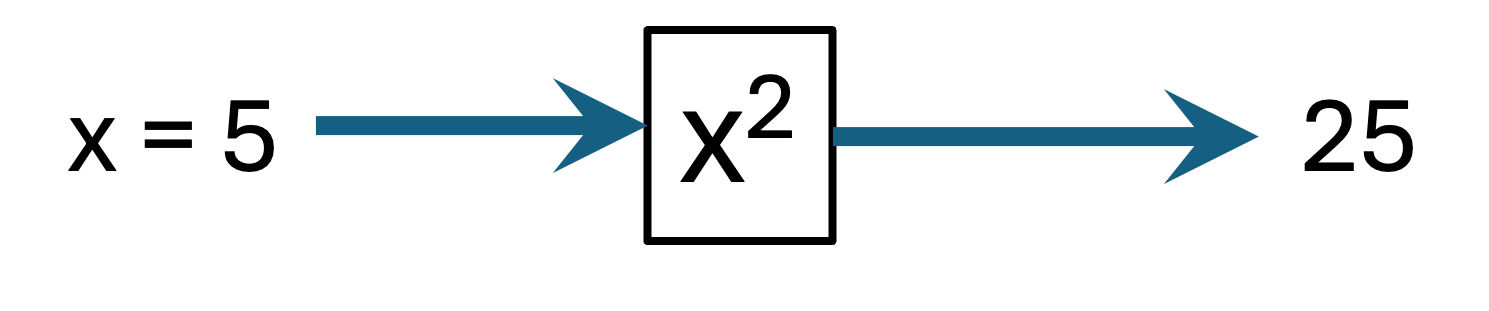
\includegraphics[width=0.7\linewidth,height=\textheight,keepaspectratio]{modules/01-data-visualization/../../images/function-1.png}

}

\caption{\label{fig-function-1}A function that squares its input}

\end{figure}%

We might have functions that take more than one input. For example, a
function might take two inputs x and y, and produce 23 + 3x + 4y as
output. Figure~\ref{fig-function-2} shows a function with two inputs.

\begin{figure}

\centering{

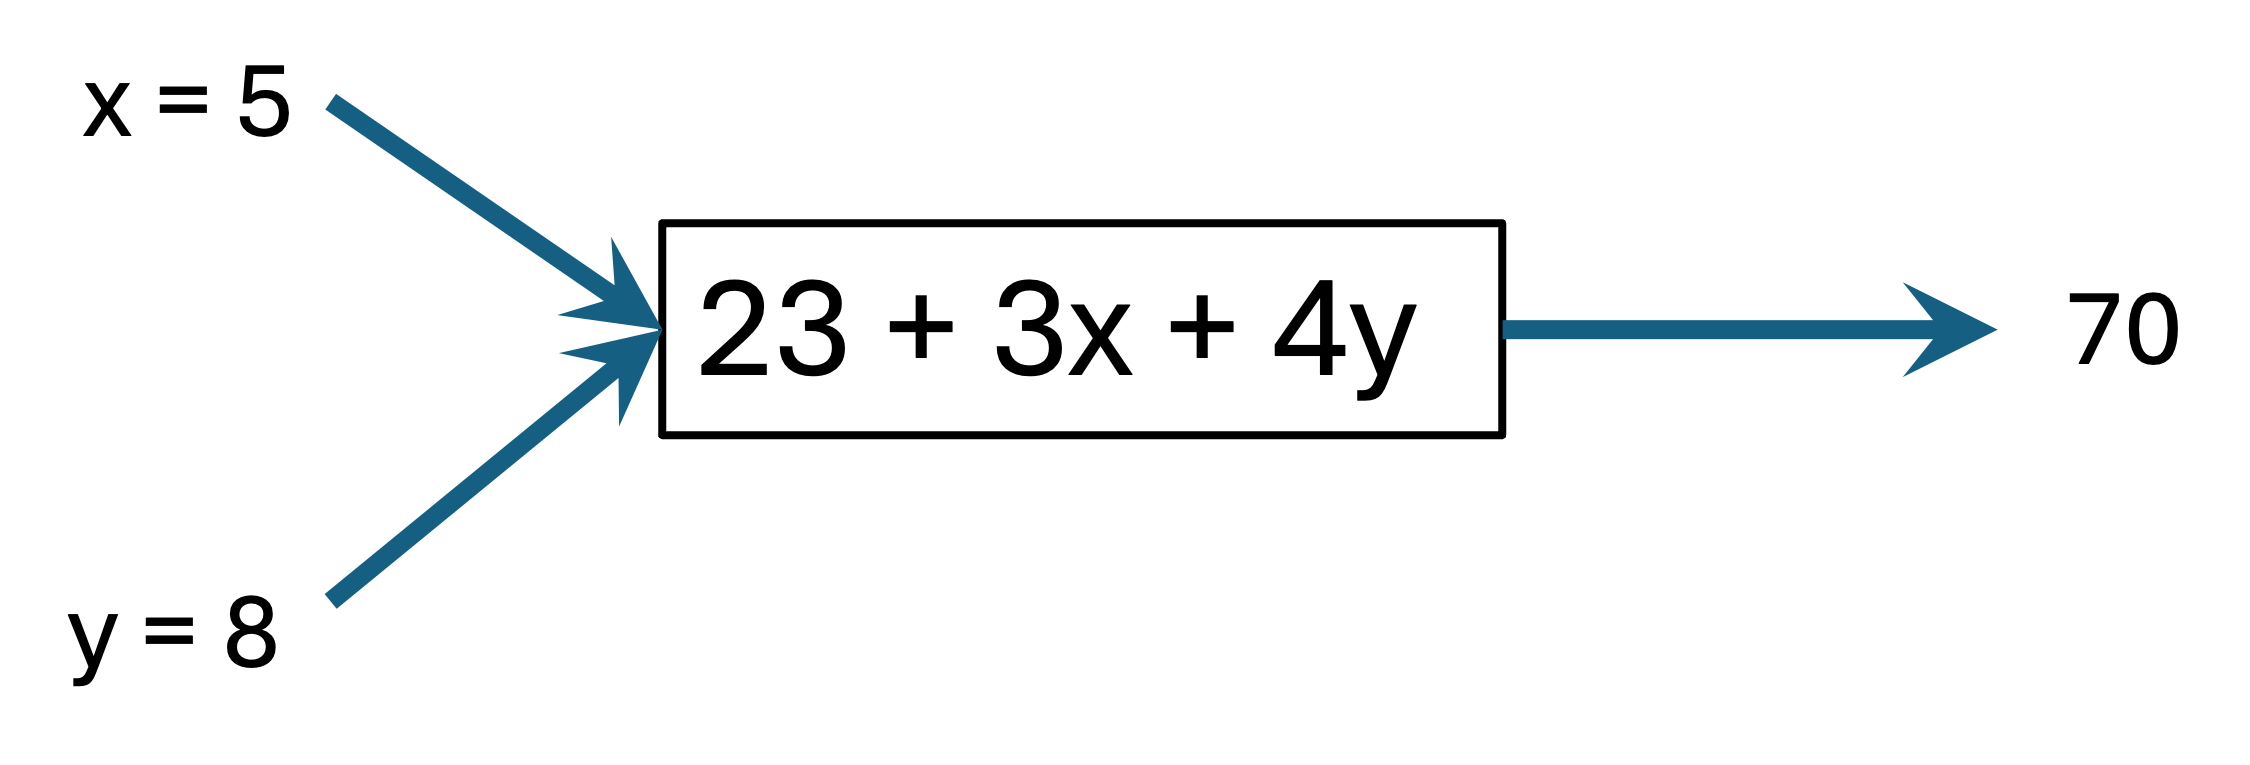
\includegraphics[width=0.7\linewidth,height=\textheight,keepaspectratio]{modules/01-data-visualization/../../images/function-2.png}

}

\caption{\label{fig-function-2}A function that computes 23+3x+4y where x
and y are its inputs}

\end{figure}%

In computing, we commonly refer to a function's inputs as its
\emph{arguments}. Figure~\ref{fig-function-3} illustrates this.

\begin{figure}

\centering{

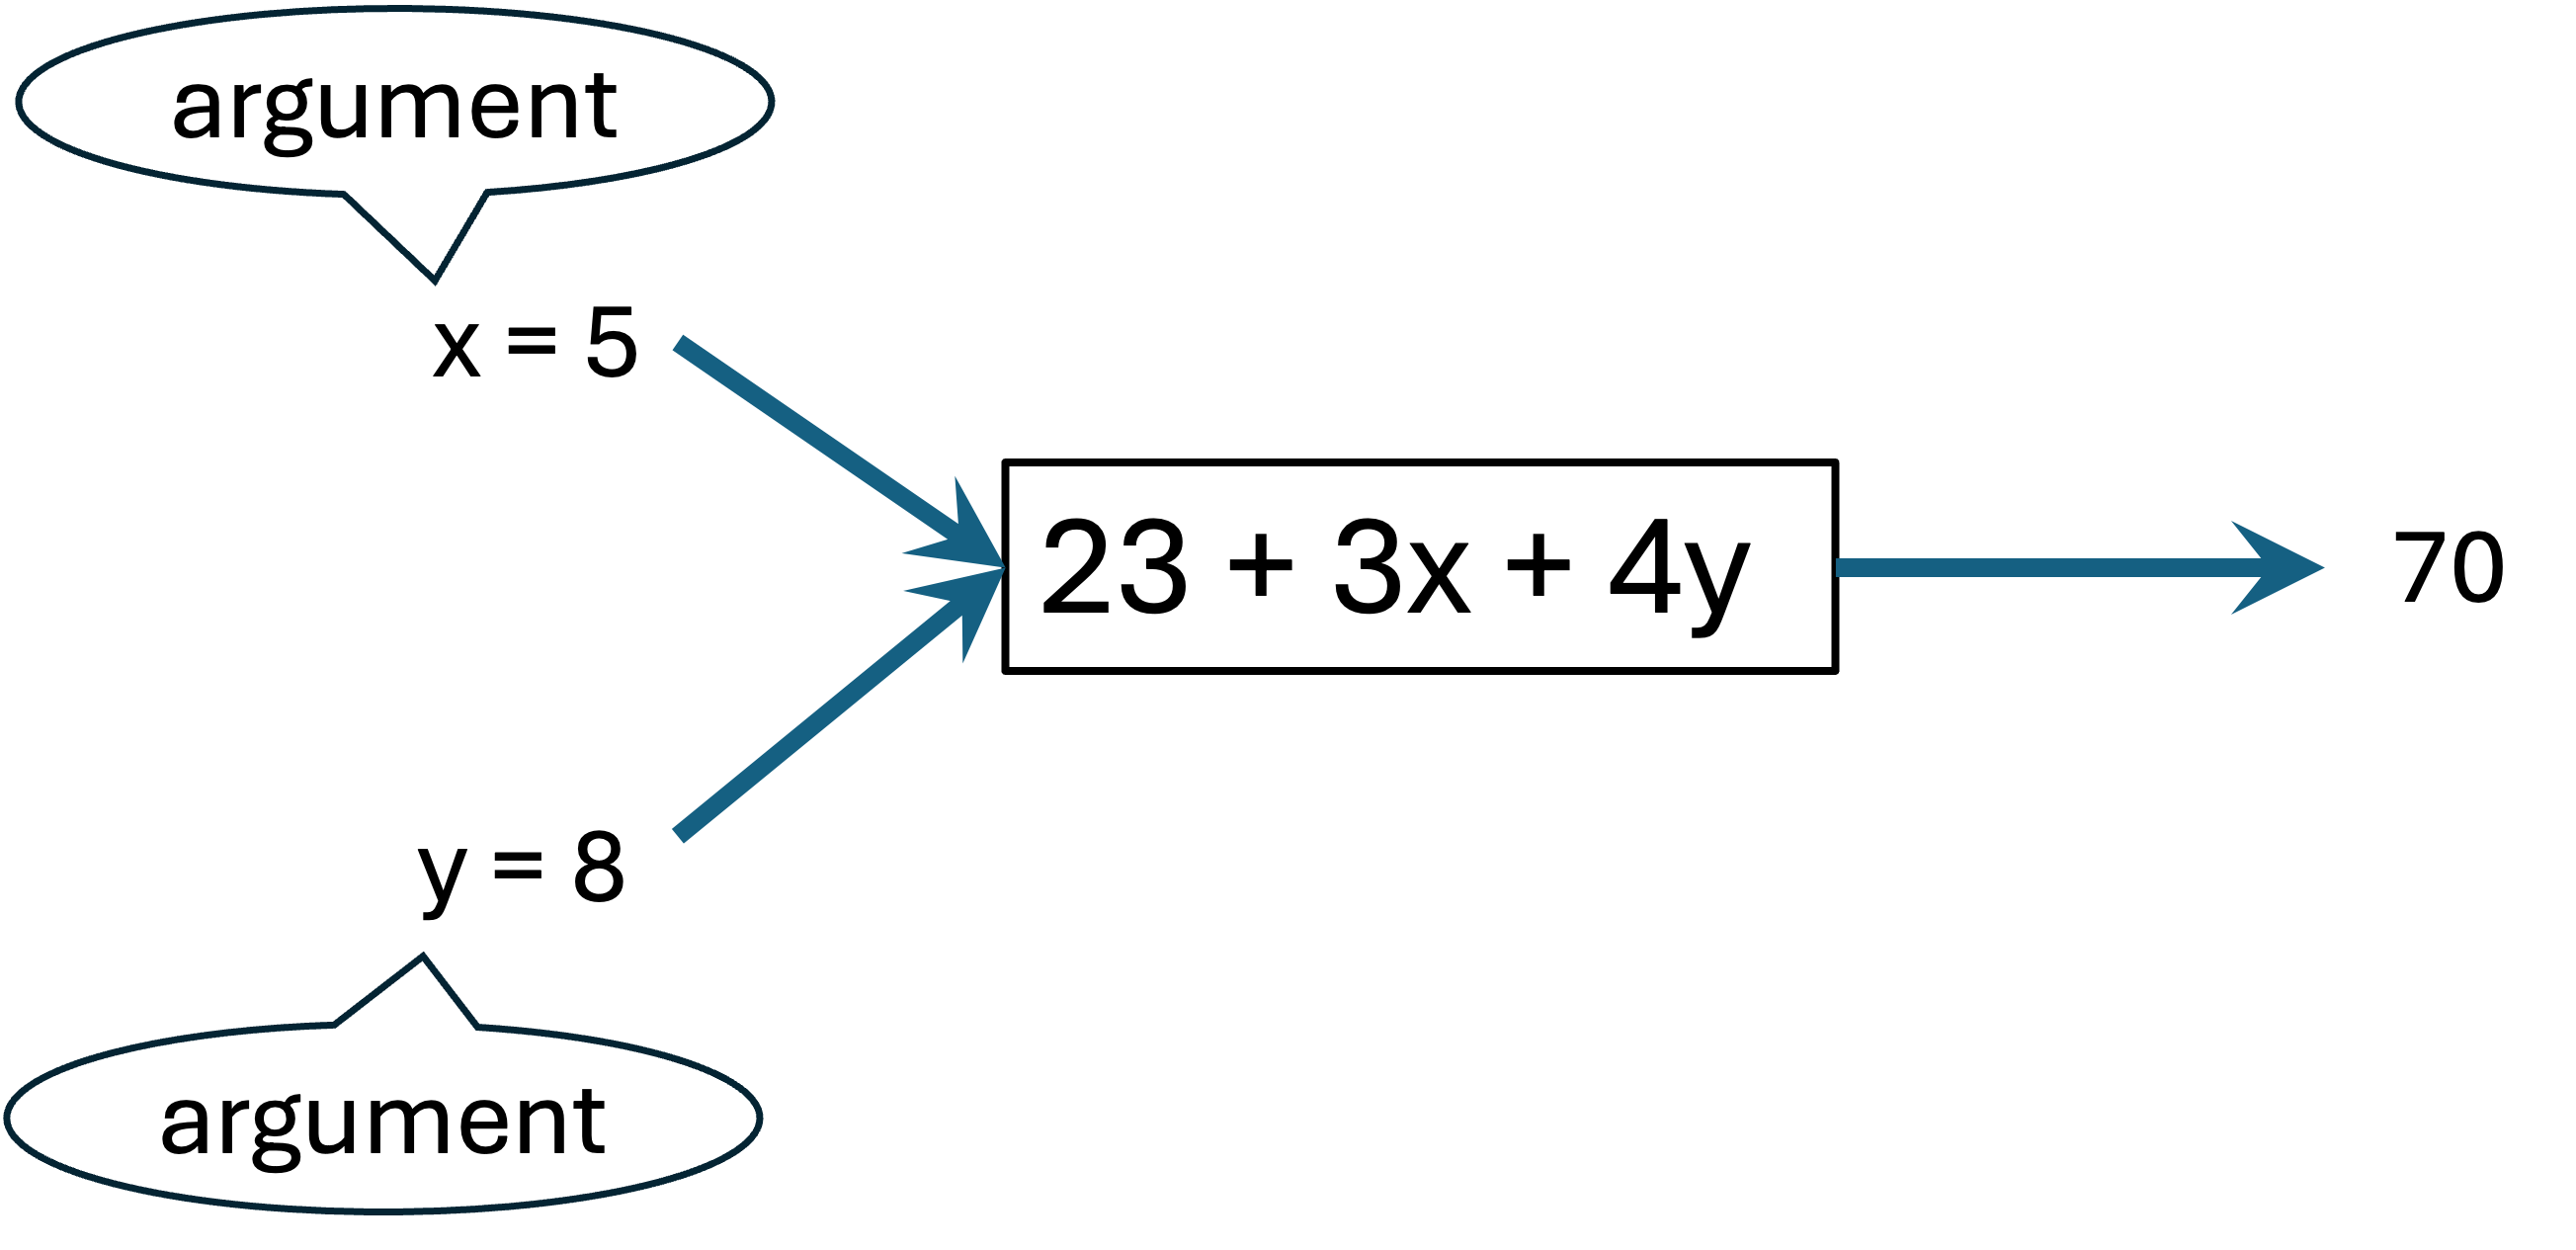
\includegraphics[width=0.7\linewidth,height=\textheight,keepaspectratio]{modules/01-data-visualization/../../images/function-3.png}

}

\caption{\label{fig-function-3}We generally refer to a function's inputs
as its \emph{arguments} -- this function has two arguments, x and y}

\end{figure}%

The functions we considered in our examples thus far in
Figure~\ref{fig-function-1}, Figure~\ref{fig-function-2}, and
Figure~\ref{fig-function-3} have been so simple that we were able to
show the actual computation in the box representing the function. Most
functions we use in real-life are more complex and we give them
evocative names. In such cases, it makes more sense to place the name of
the function in the box. Figure~\ref{fig-function-4} shows a generic
representation of a function named \emph{cost} with three arguments
named \emph{arg1}, \emph{arg2}, and \emph{arg3}.

\begin{figure}

\centering{

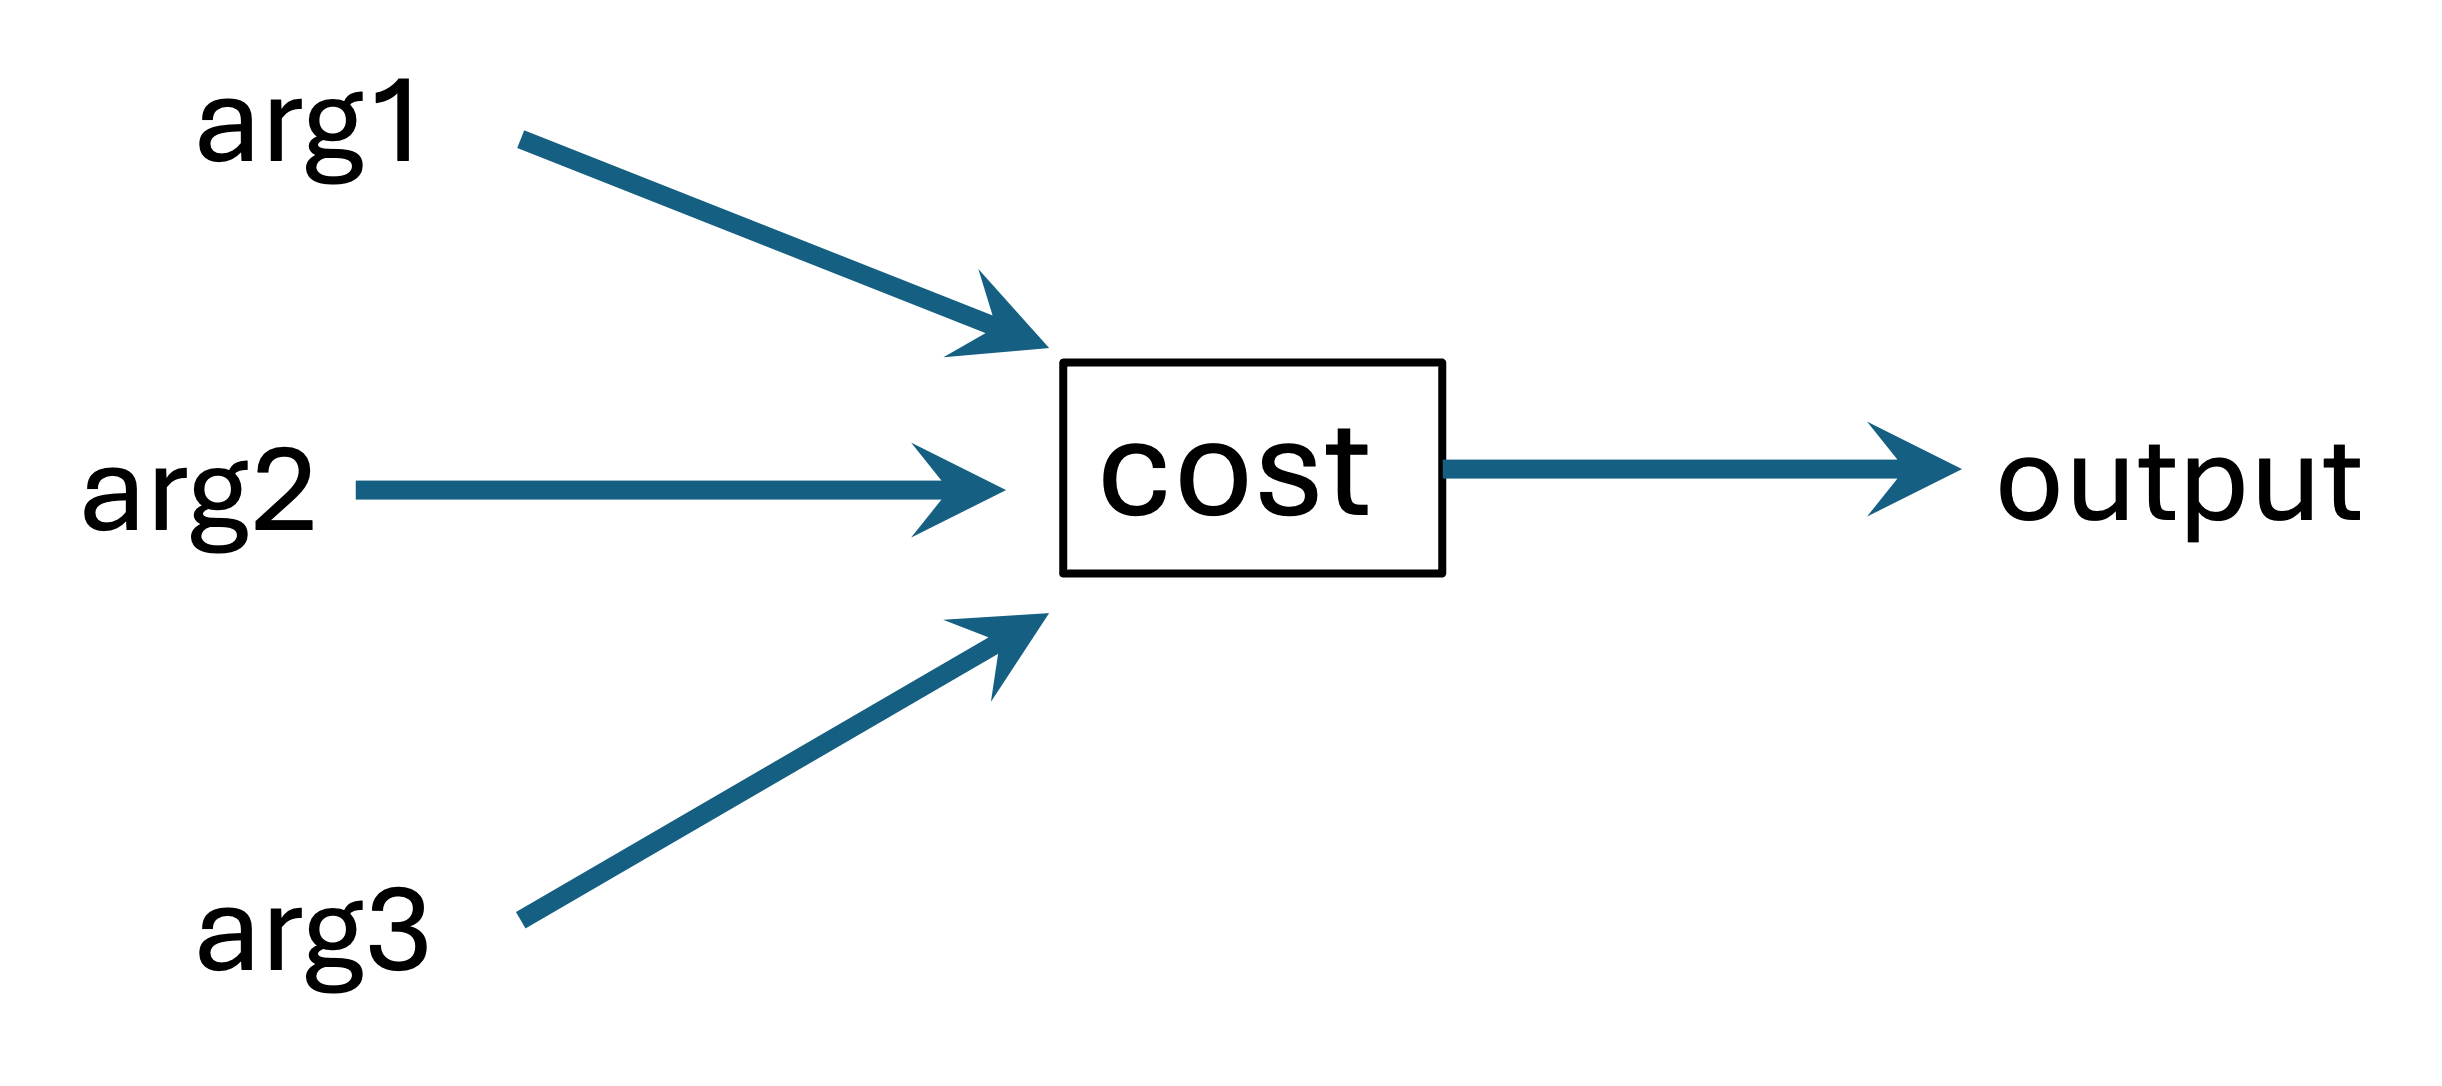
\includegraphics[width=0.7\linewidth,height=\textheight,keepaspectratio]{modules/01-data-visualization/../../images/function-4.png}

}

\caption{\label{fig-function-4}Pictorial representation of a function
named \emph{cost} that has three arguments}

\end{figure}%

When we use a function to perform some computation, we are said to
\emph{invoke} the function. We generally invoke a function by using its
name and by supplying the argument values in parentheses, as
Figure~\ref{fig-function-5} shows. We also use the term \emph{passing
arguments} to functions to refer to the act of supplying the inputs to a
function. We also refer to the result of a function as its \emph{return
value}. We will also speak of a function as \emph{returning} something.
Figure~\ref{fig-function-5} also shows that a function argument can be
numeric or non-numeric.

\begin{figure}

\centering{

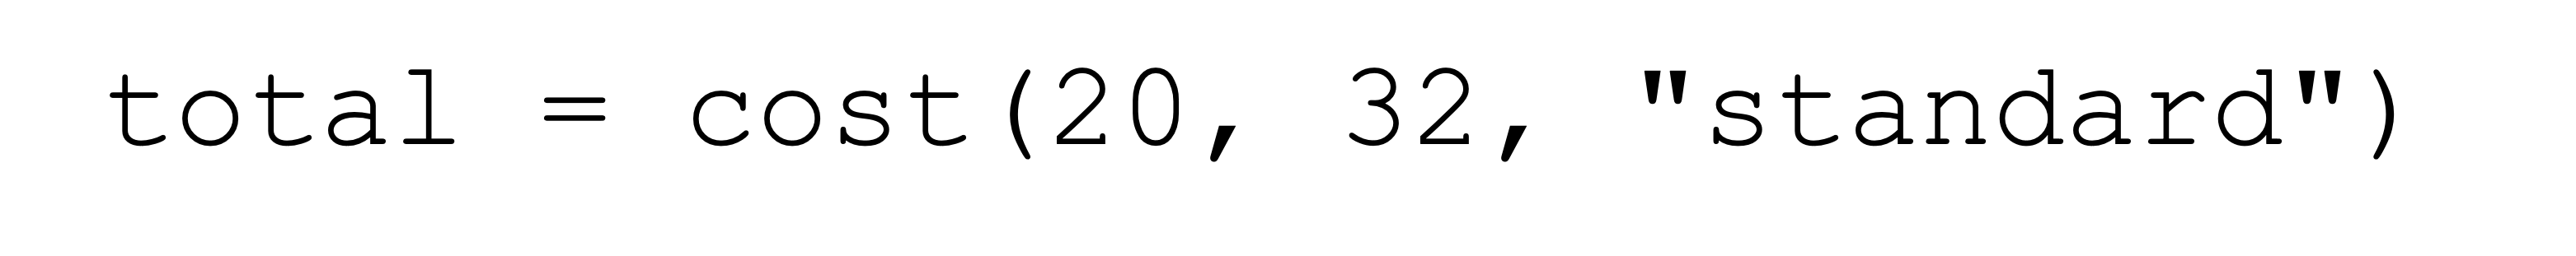
\includegraphics[width=0.7\linewidth,height=\textheight,keepaspectratio]{modules/01-data-visualization/../../images/function-5.png}

}

\caption{\label{fig-function-5}Invoking a named function and storing the
function's return value in a variable named \emph{total}}

\end{figure}%

In the next section, we look at using functions to perform computing in
R. At that time we will look at a different way of passing arguments to
functions.

Almost all forms of computing, including statistical computing, make
significant use of functions. In this course, many of the functions we
use take data frame as input and produce a data frame as output. Let us
now look at how we use functions in R to work with data and to perform
statistical computations.

\section{Using R functions}\label{using-r-functions}

We will now look at some common R functions that we will use repeatedly
in this course.

\subsection{\texorpdfstring{\emph{nrow}}{nrow}}\label{nrow}

We will consider the \emph{nrow()} function that allows us to find how
many rows a data frame contains. We pass a data frame as argument to the
\emph{nrow()} function and it returns a number specifying how many rows
the argument data frame has. For example, to find how many rows the
\emph{Boston\_marathon} data frame has, we can use the following code.

\begin{lstlisting}[language=R]
nrow(Boston_marathon)
\end{lstlisting}

\begin{lstlisting}
[1] 175
\end{lstlisting}

In the code above, we used the style of function invocation that
Figure~\ref{fig-function-5} introduced.

\subsection{\texorpdfstring{The \emph{pipe}
operator}{The pipe operator}}\label{the-pipe-operator}

In this course we also use another method of passing an argument to a
function -- via \emph{pipes}. W first see the code and then dissect it.
We will invoke the \emph{nrow()} function again, but using a different
approach. Like the previous code, this also finds the number of rows in
the \emph{Boston\_marathon} data frame.

\begin{lstlisting}[language=R]
Boston_marathon |> nrow()
\end{lstlisting}

\begin{lstlisting}
[1] 175
\end{lstlisting}

In the code above, we are still passing the Boston\_marathon data frame
as an argument to the \emph{nrow()} function, but we are passing it
along a \emph{pipe} which appears in the code as
``\textbar\textgreater{}''.

Figure~\ref{fig-pipe-1} explains the different components in the code.

\begin{figure}

\centering{

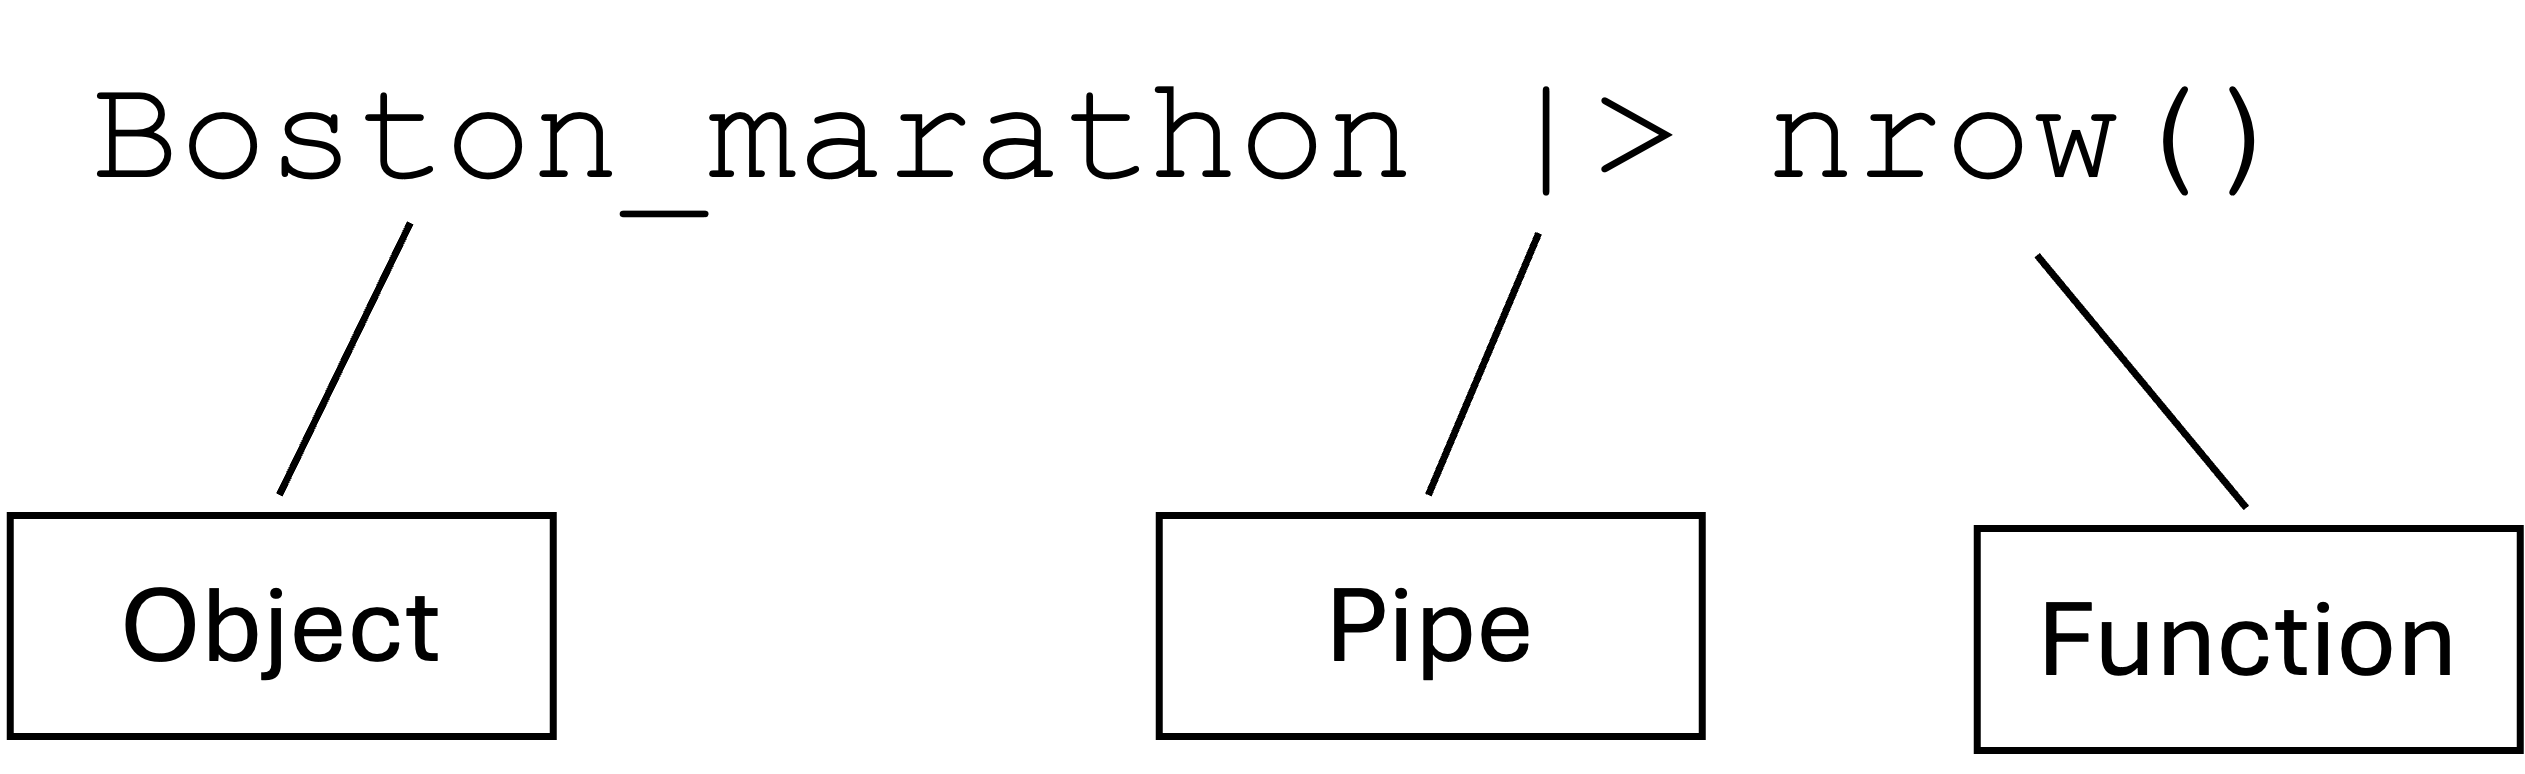
\includegraphics[width=0.7\linewidth,height=\textheight,keepaspectratio]{modules/01-data-visualization/../../images/pipe-1.png}

}

\caption{\label{fig-pipe-1}Using the pipe operator to supply the
Boston\_marathon data frame as an argument to the norw function}

\end{figure}%

The pipe operator ``\textbar\textgreater{}'' has the effect of
\emph{injecting} whatever appears on its left hand side as an argument
to the function on the right hand side. Figure~\ref{fig-pipe-2} makes
this very explicit by literally depicting the pipe operator
``\textbar\textgreater{}'' as a physical pipe.

\begin{figure}

\centering{

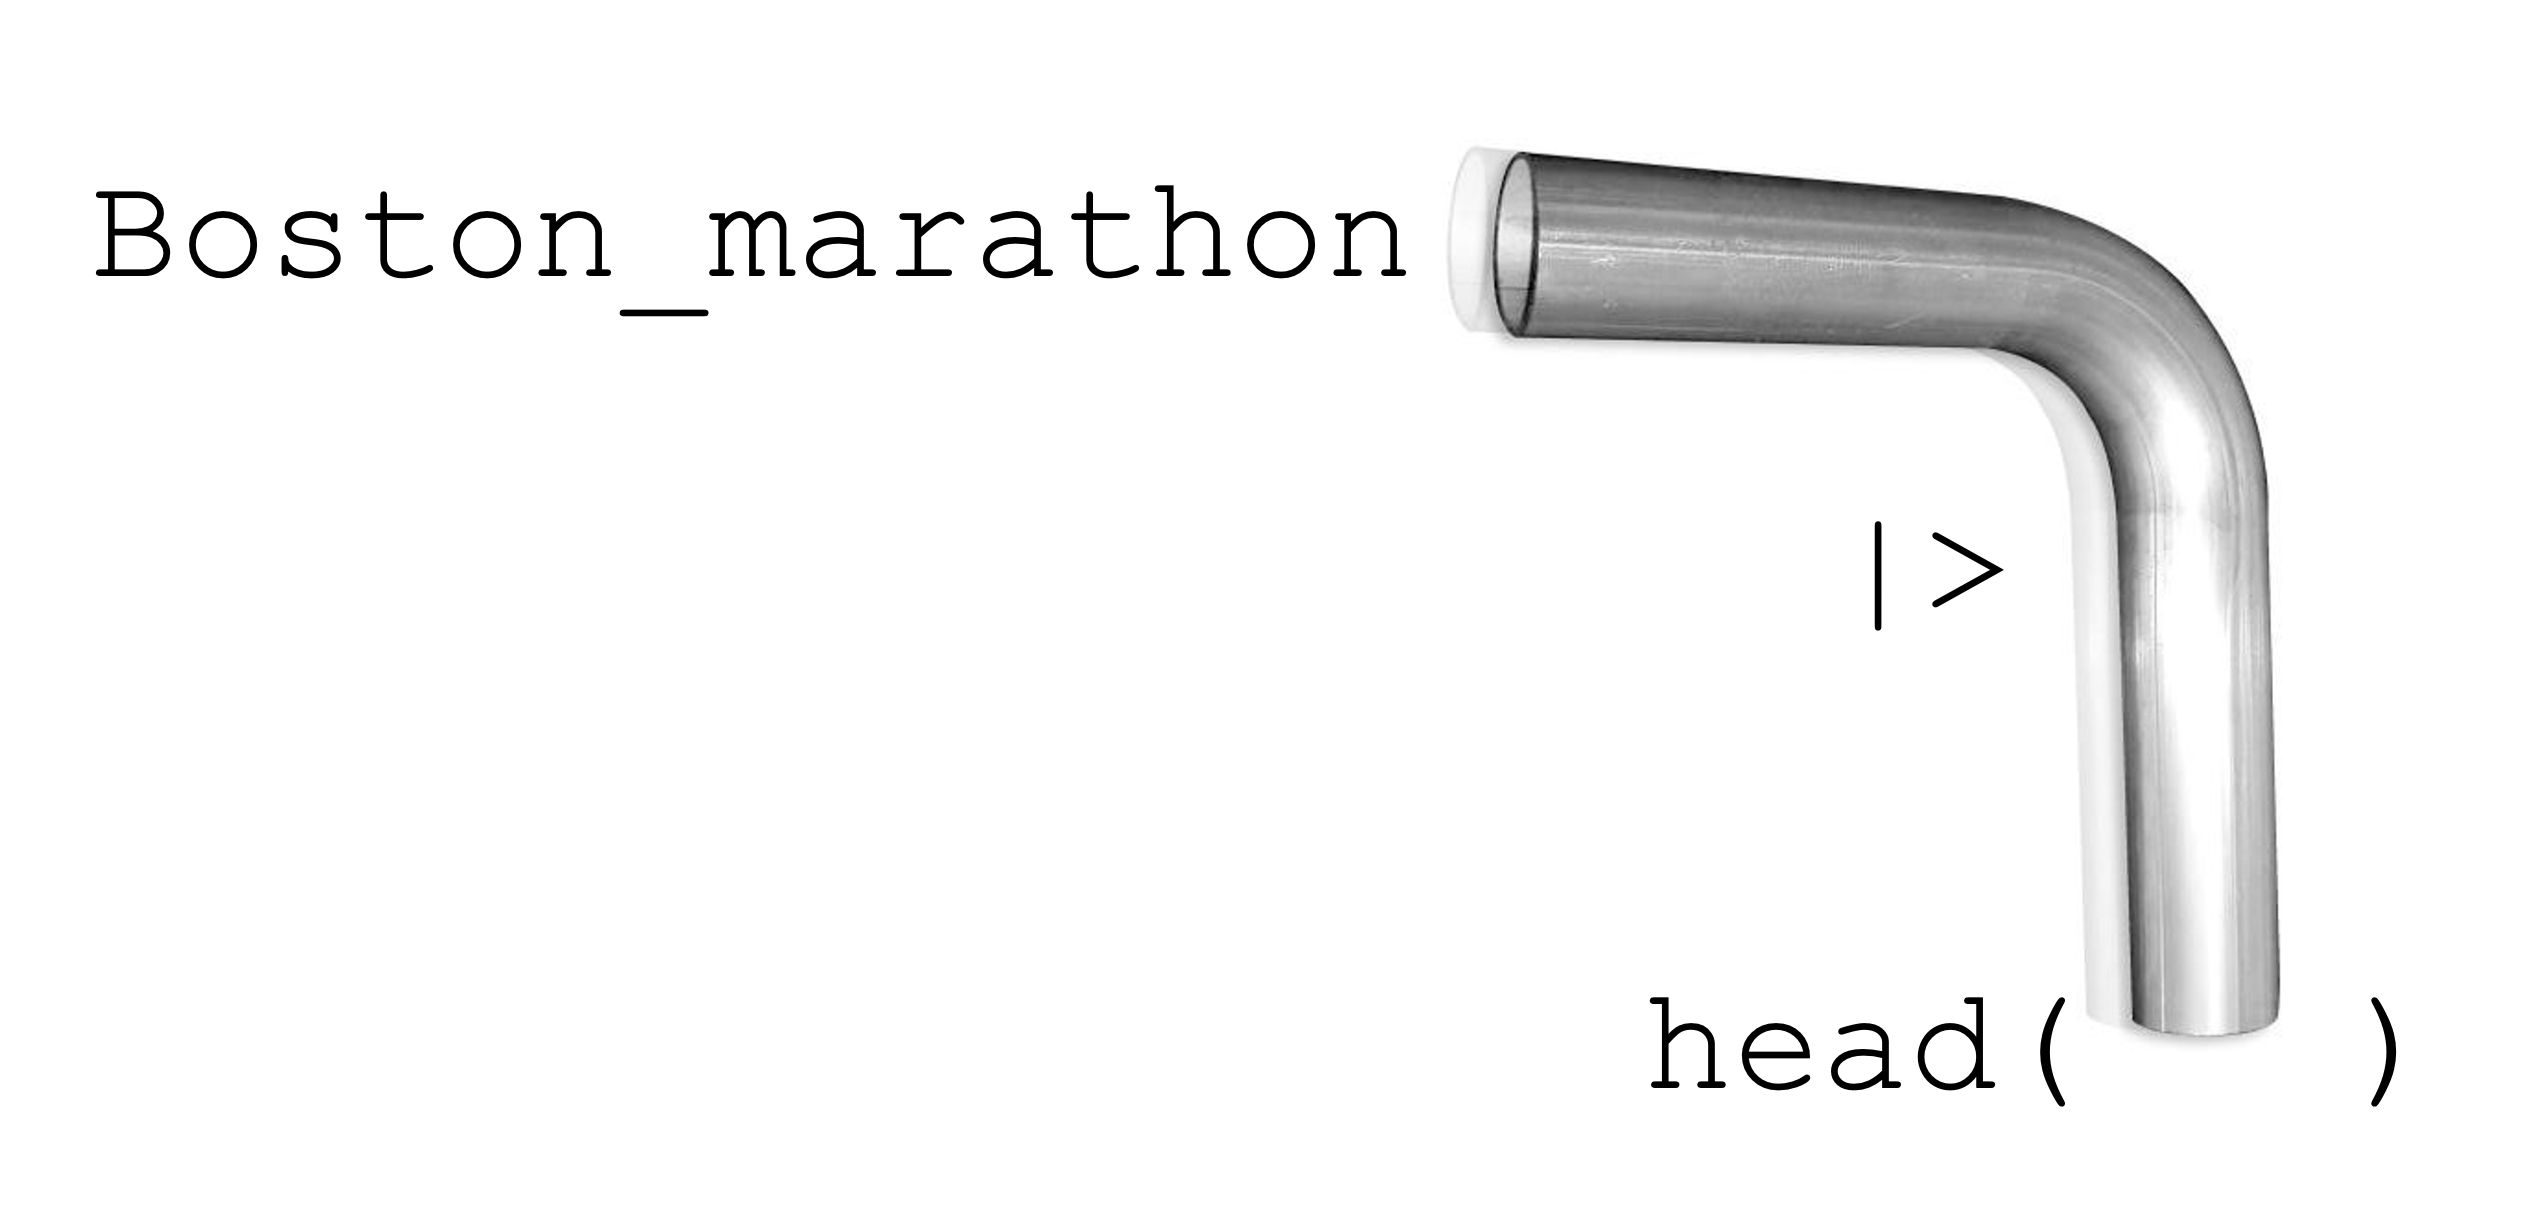
\includegraphics[width=0.7\linewidth,height=\textheight,keepaspectratio]{modules/01-data-visualization/../../images/pipe-2.png}

}

\caption{\label{fig-pipe-2}Seeing the pipe operator literally as a pipe
though which the argument flows into a function}

\end{figure}%

Going forward, we will use this \emph{pipe} approach extensively, but
also mix in the earlier approach in some places. You will easily adjust
to our patterns.

\subsection{\texorpdfstring{\emph{ncol}}{ncol}}\label{ncol}

We can use the \emph{ncol()} function to find the number of columns in a
data frame.

\begin{lstlisting}[language=R]
Boston_marathon |> ncol()
\end{lstlisting}

\begin{lstlisting}
[1] 6
\end{lstlisting}

The above shows us that the \emph{Boston\_marathon} data frame has 6
columns or variables.

\subsection{\texorpdfstring{\emph{head}}{head}}\label{head}

You can use the \emph{head()} function to preview the first several rows
of a data frame. This time we will use the \emph{Births2022} data frame
from the \emph{LSTbook} package.

\begin{lstlisting}[language=R]
Births2022 |> head()
\end{lstlisting}

\begin{lstlisting}
# A tibble: 6 x 38
  month dow   place  paternity meduc feduc married
  <chr> <ord> <chr>  <chr>     <ord> <ord> <chr>  
1 05    Sat   hospi~ <NA>      Assoc HS    NA     
2 09    Mon   hospi~ <NA>      <NA>  <NA>  NA     
3 06    Thurs hospi~ N         HS    <NA>  not_ma~
4 05    Thurs hospi~ Y         Mast~ Bach~ married
5 08    Thurs hospi~ <NA>      HS    HS    NA     
6 01    Tues  hospi~ Y         HS    <NA>  not_ma~
# i 31 more variables: fage <dbl>, mage <dbl>,
#   total_kids <int>, interval <ord>,
#   prenatal_start <ord>, prenatal_visits <dbl>,
#   mheight <dbl>, wt_pre <dbl>,
#   wt_delivery <dbl>, diabetes_pre <chr>,
#   diabetes_gest <chr>, hbp_pre <chr>,
#   hbp_gest <chr>, eclampsia <chr>, ...
\end{lstlisting}

The above previewed the first six rows of \emph{Births2022} by default
because we did not specify how many rows we wanted. We can specify that
explicitly. The following previews the first 10 rows.

\begin{lstlisting}[language=R]
Births2022 |> head(10)
\end{lstlisting}

\begin{lstlisting}
# A tibble: 10 x 38
   month dow   place paternity meduc feduc married
   <chr> <ord> <chr> <chr>     <ord> <ord> <chr>  
 1 05    Sat   hosp~ <NA>      Assoc HS    NA     
 2 09    Mon   hosp~ <NA>      <NA>  <NA>  NA     
 3 06    Thurs hosp~ N         HS    <NA>  not_ma~
 4 05    Thurs hosp~ Y         Mast~ Bach~ married
 5 08    Thurs hosp~ <NA>      HS    HS    NA     
 6 01    Tues  hosp~ Y         HS    <NA>  not_ma~
 7 07    Mon   hosp~ <NA>      <NA>  <NA>  NA     
 8 11    Thurs hosp~ <NA>      Bach~ Bach~ NA     
 9 03    Sat   hosp~ <NA>      HS+   <NA>  NA     
10 08    Fri   hosp~ <NA>      Bach~ Bach~ NA     
# i 31 more variables: fage <dbl>, mage <dbl>,
#   total_kids <int>, interval <ord>,
#   prenatal_start <ord>, prenatal_visits <dbl>,
#   mheight <dbl>, wt_pre <dbl>,
#   wt_delivery <dbl>, diabetes_pre <chr>,
#   diabetes_gest <chr>, hbp_pre <chr>,
#   hbp_gest <chr>, eclampsia <chr>, ...
\end{lstlisting}

\subsection{\texorpdfstring{\emph{names}}{names}}\label{names}

We use this to find the names of the columns in a data frame.

\begin{lstlisting}[language=R]
Births2022 |> names()
\end{lstlisting}

\begin{lstlisting}
 [1] "month"           "dow"            
 [3] "place"           "paternity"      
 [5] "meduc"           "feduc"          
 [7] "married"         "fage"           
 [9] "mage"            "total_kids"     
[11] "interval"        "prenatal_start" 
[13] "prenatal_visits" "mheight"        
[15] "wt_pre"          "wt_delivery"    
[17] "diabetes_pre"    "diabetes_gest"  
[19] "hbp_pre"         "hbp_gest"       
[21] "eclampsia"       "induction"      
[23] "augmentation"    "anesthesia"     
[25] "presentation"    "method"         
[27] "trial_at_labor"  "attendant"      
[29] "payment"         "apgar5"         
[31] "apgar10"         "plurality"      
[33] "sex"             "duration"       
[35] "menses"          "weight"         
[37] "living"          "breastfed"      
\end{lstlisting}

\subsection{\texorpdfstring{\emph{summarize}}{summarize}}\label{sec-summarize-function}

We often calculate summaries (like the average of a variable) of the
data contained in a data frame.

The code below shows how to compute the average of the \emph{time}
variable in the \emph{Boston\_marathon} data frame.

\begin{lstlisting}[language=R]
Boston_marathon |> 
  summarize(avg_time = mean(time))
\end{lstlisting}

\begin{lstlisting}
# A tibble: 1 x 1
  avg_time 
  <drtn>   
1 8635 secs
\end{lstlisting}

In the above code, we passed the \emph{Boston\_marathon} data frame via
a pipe to the \emph{summarize} function. Within the \emph{summarize}
function, we have used the R function \emph{mean} to compute the average
by passing the variable \emph{time} as an argument to the \emph{mean}
function. Note that we did not use the \emph{pipe} to pass an argument
to the \emph{mean} function.

We chose to name the return value from the \emph{mean} function as
\emph{average time}. You do not necessarily need to name the summaries
we compute in the \emph{summarize} function, but we strongly recommend
it.

At appropriate points in the course, we will discuss other examples of
summaries. We will see \emph{variance}, \emph{standard deviation}, and,
\emph{correlation coefficient}, among others, at appropriate points in
the course.

For most of the summaries we compute we will use the general
\emph{summarize} function. Within the \emph{summarize} function, we use
specific functions depending on the kind of summary we compute. In the
previous example, we used the \emph{mean} function for the average.
Later we will see other functions to use within the \emph{summarize}
function.

\subsection{\texorpdfstring{\emph{count}}{count}}\label{count}

The \emph{count()} function comes in handy when we want to count how
many occurrences of each distinct value are present in a variable. For
example, suppose we want to find how many rows are there for each
\emph{sex} in the \emph{Boston\_marathon} data frame, we can do the
following.

\begin{lstlisting}[language=R]
Boston_marathon |> count(sex)
\end{lstlisting}

\begin{lstlisting}
# A tibble: 2 x 2
  sex        n
  <chr>  <int>
1 female    50
2 male     125
\end{lstlisting}

Similarly, if we wanted to find out how many times each \emph{country}
occurs, we can do this.

\begin{lstlisting}[language=R]
Boston_marathon |> count(country)
\end{lstlisting}

\begin{lstlisting}
# A tibble: 25 x 2
   country               n
   <chr>             <int>
 1 Australia             1
 2 Belgium               2
 3 Canada               17
 4 Colombia              1
 5 Comm. Ind. States     1
 6 England               3
 7 Ethiopia             14
 8 Finland               7
 9 Germany               6
10 Greece                2
# i 15 more rows
\end{lstlisting}

As you can see, the \emph{count()} function comes in handy when a
variable is categorical. It also works for numerical variables, but will
apply much more rarely in these cases.

\section{\texorpdfstring{Missing values
(\emph{NA}s)}{Missing values (NAs)}}\label{sec-missing-values}

Suppose the HR department of a company has a data frame of information
about employees with variables (columns) \emph{employee\_id},
\emph{first\_name}, \emph{last\_name}, \emph{base\_salary},
\emph{phone\_no}, and \emph{base\_office}. It is not essential that we
have data on every variable for every row. For example, it could be the
case that the company does not have a \emph{phone\_no} for some
employees and does not have a \emph{base\_office} for some. These are
called \emph{missing values}. A missing value denotes something whose
value \emph{we do not know}. A missing value is not the same as a blank
character value or a zero numeric value. Blanks and zeros are valid and
known values for variables. A \emph{missing value is different} --
\emph{we do not know the value}.

Table~\ref{tbl-no-missing-values} shows a data frame with \textbf{no
missing values}. In each row, we see values for every variable.

\begin{longtable}[]{@{}lrr@{}}

\caption{\label{tbl-no-missing-values}A data frame with no missing
values -- in every row, every variable has a value}

\tabularnewline

\toprule\noalign{}
channel & advertising\_spend\_k & weekly\_sales\_k \\
\midrule\noalign{}
\endhead
\bottomrule\noalign{}
\endlastfoot
Search Ads & 28.1 & 152 \\
Search Ads & 30.6 & 152 \\
Search Ads & 93.4 & 369 \\
Search Ads & 51.3 & 289 \\
Retail Promo & 54.6 & 175 \\
Search Ads & 86.6 & 342 \\
Retail Promo & 46.5 & 169 \\
Retail Promo & 41.4 & 142 \\
Search Ads & 78.1 & 322 \\
Retail Promo & 41.1 & 182 \\

\end{longtable}

On the other hand Table~\ref{tbl-missing-values} shows a small data
frame \textbf{with missing values}.

\begin{longtable}[]{@{}
  >{\raggedleft\arraybackslash}p{(\linewidth - 10\tabcolsep) * \real{0.1558}}
  >{\raggedright\arraybackslash}p{(\linewidth - 10\tabcolsep) * \real{0.1429}}
  >{\raggedright\arraybackslash}p{(\linewidth - 10\tabcolsep) * \real{0.1299}}
  >{\raggedleft\arraybackslash}p{(\linewidth - 10\tabcolsep) * \real{0.1558}}
  >{\raggedright\arraybackslash}p{(\linewidth - 10\tabcolsep) * \real{0.2338}}
  >{\raggedright\arraybackslash}p{(\linewidth - 10\tabcolsep) * \real{0.1818}}@{}}

\caption{\label{tbl-missing-values}A data frame with missing values --
the \emph{NA}s in columns \emph{phone\_no} and \emph{base\_office}
represent missing values}

\tabularnewline

\toprule\noalign{}
\begin{minipage}[b]{\linewidth}\raggedleft
employee\_id
\end{minipage} & \begin{minipage}[b]{\linewidth}\raggedright
first\_name
\end{minipage} & \begin{minipage}[b]{\linewidth}\raggedright
last\_name
\end{minipage} & \begin{minipage}[b]{\linewidth}\raggedleft
base\_salary
\end{minipage} & \begin{minipage}[b]{\linewidth}\raggedright
phone\_no
\end{minipage} & \begin{minipage}[b]{\linewidth}\raggedright
base\_office
\end{minipage} \\
\midrule\noalign{}
\endhead
\bottomrule\noalign{}
\endlastfoot
10210 & Betty & Chu & 67000 & +1 (777) 555-1212 & New Jersey \\
24532 & Jason & Fingleton & 85000 & +1 (732) 555-1212 & NA \\
56437 & Shim & Sung & 76000 & NA & New York \\
20320 & Ravi & Shankar & 100000 & +91 81487 03210 & New Delhi \\
67582 & Emily & Weitz & 87000 & NA & San Francisco \\

\end{longtable}

\section{Codebook}\label{codebook}

Before using a data frame, we need to understand it well. That means, at
the very least, that we know the \emph{unit of observation}, the meaning
of each \emph{variable} and the \emph{units of measurement} for a
variable where applicable. The \emph{codebook} for a data frame provides
this information. You can use the ? operator for this purpose as the
example code below shows.

\begin{lstlisting}[language=R]
?Boston_marathon
\end{lstlisting}

This command will show the codebook in the bottom right pane of RStudio.

\chapter{Exploring Relationships through
Scatterplots}\label{sec-visualizing-relationships}

This chapter covers the basics of generating and interpreting
scatterplots.

The term \emph{statistics} often conjures up thoughts of numerical
computations. However, before we perform various computations, we often
get a feel for the data and the underlying patterns by first visualizing
the data. In this course we will use only a few standard plots to
communicate essential statistical ideas.

In fact, use a single function -- \emph{point\_plot} -- to generate all
of our plots. Although R offers numerous, sophisticated plotting
features to plot almost anything we can imagine, we will keep things
simple and focus only on what we need to support the concepts that our
course covers.

\section*{Learning outcomes}\label{learning-outcomes-1}
\addcontentsline{toc}{section}{Learning outcomes}

\markright{Learning outcomes}

\textbf{Interpret point plots} - Explain what a point means (x value and
y value). - Map between plot ↔ row in a data frame. - Describe
direction/strength/absence of relationship.

\textbf{Use R to generate point plots}

\begin{itemize}
\tightlist
\item
  Use point\_plot(y \textasciitilde{} x) for numeric--numeric and
  point\_plot(y \textasciitilde{} x\_cat) for numeric--categorical.
\item
  Use + color\_var and + facet\_var in the formula.
\end{itemize}

\textbf{Explain and interpret correlation} - Explain what correlation
measures (direction + strength of linear association) and interpret
sign/magnitude.

\section{Plotting the relationship between two numerical
variables}\label{plotting-the-relationship-between-two-numerical-variables}

We will rely extensively on a single plotting function named
\emph{point\_plot()}. It lives in the \emph{LSTbook} package. We will be
loading both the \emph{LSTbook} package and the \emph{LSTextra}s
package. Once we load these packages the \emph{point\_plot()} function
becomes available for us to use.

Let us first look at the \emph{price\_demand} data frame that is built
into the \emph{LSTextras} package and is therefore available as soon as
you load the package.

A hypothetical company has gathered data for a single product. Over
time, and across very similar sales areas, the company has charged
different prices for the same product, It has recorded the monthly sales
for each price. The data frame \emph{price\_demand} contains the price
and the corresponding sales quantities. We would like to study if the
two variables \emph{price} and \emph{sales\_qty} are related in any way.

First let us see some rows from the data frame.

\begin{longtable}[t]{rr}

\caption{\label{tbl-price-demand}Price Demand data (first 15 rows)}

\tabularnewline

\toprule
price & sales\_qty\\
\midrule
11.8 & 1260\\
12.1 & 1215\\
13.6 & 1214\\
12.3 & 1298\\
12.4 & 1160\\
\addlinespace
13.7 & 1138\\
12.6 & 1174\\
11.2 & 1220\\
11.7 & 1313\\
11.9 & 1283\\
\addlinespace
13.3 & 1170\\
12.6 & 1247\\
12.6 & 1283\\
12.3 & 1263\\
11.8 & 1259\\
\bottomrule

\end{longtable}

The full data frame has 500 rows. With so many rows, we cannot easily
get a handle on the overall pattern by looking at the data directly.
Visualizing the data might help us. We will do several things in this
section:

\begin{itemize}
\tightlist
\item
  generate the plot using R code
\item
  understand how each element of the plot is related to the original
  data frame
\item
  understand the various elements of the code so that you can use
  similar code to generate plots that you many need
\item
  interpret the plot
\end{itemize}

\begin{tcolorbox}[enhanced jigsaw, colback=white, leftrule=.75mm, toprule=.15mm, bottomtitle=1mm, breakable, coltitle=black, toptitle=1mm, title={Quick Check}, opacitybacktitle=0.6, colbacktitle=quarto-callout-note-color!10!white, arc=.35mm, left=2mm, colframe=quarto-callout-note-color-frame, titlerule=0mm, rightrule=.15mm, bottomrule=.15mm, opacityback=0]

In the \emph{price\_demand} data frame, what does one row represent?

\end{tcolorbox}

\begin{tcolorbox}[enhanced jigsaw, colback=white, leftrule=.75mm, toprule=.15mm, bottomtitle=1mm, breakable, coltitle=black, toptitle=1mm, title={Suggested answer}, opacitybacktitle=0.6, colbacktitle=quarto-callout-note-color!10!white, arc=.35mm, left=2mm, colframe=quarto-callout-note-color-frame, titlerule=0mm, rightrule=.15mm, bottomrule=.15mm, opacityback=0]

The price charged during a particular month and the corresponding sales
quantity..

\end{tcolorbox}

\begin{tcolorbox}[enhanced jigsaw, colback=white, leftrule=.75mm, toprule=.15mm, bottomtitle=1mm, breakable, coltitle=black, toptitle=1mm, title={Quick Check}, opacitybacktitle=0.6, colbacktitle=quarto-callout-note-color!10!white, arc=.35mm, left=2mm, colframe=quarto-callout-note-color-frame, titlerule=0mm, rightrule=.15mm, bottomrule=.15mm, opacityback=0]

In the \emph{price\_demand} data frame, which variable does a company
have control over or that it can set and which one is the outcome
variable?

\end{tcolorbox}

\begin{tcolorbox}[enhanced jigsaw, colback=white, leftrule=.75mm, toprule=.15mm, bottomtitle=1mm, breakable, coltitle=black, toptitle=1mm, title={Suggested answer}, opacitybacktitle=0.6, colbacktitle=quarto-callout-note-color!10!white, arc=.35mm, left=2mm, colframe=quarto-callout-note-color-frame, titlerule=0mm, rightrule=.15mm, bottomrule=.15mm, opacityback=0]

\emph{price} is the input/explanatory variable; \emph{sales quantity} is
the outcome/response

\end{tcolorbox}

\begin{tcolorbox}[enhanced jigsaw, colback=white, leftrule=.75mm, toprule=.15mm, bottomtitle=1mm, breakable, coltitle=black, toptitle=1mm, title={Quick Check}, opacitybacktitle=0.6, colbacktitle=quarto-callout-note-color!10!white, arc=.35mm, left=2mm, colframe=quarto-callout-note-color-frame, titlerule=0mm, rightrule=.15mm, bottomrule=.15mm, opacityback=0]

If the data frame has 500 rows, how many (price, sales\_qty) pairs
exist?

\end{tcolorbox}

\begin{tcolorbox}[enhanced jigsaw, colback=white, leftrule=.75mm, toprule=.15mm, bottomtitle=1mm, breakable, coltitle=black, toptitle=1mm, title={Suggested answer}, opacitybacktitle=0.6, colbacktitle=quarto-callout-note-color!10!white, arc=.35mm, left=2mm, colframe=quarto-callout-note-color-frame, titlerule=0mm, rightrule=.15mm, bottomrule=.15mm, opacityback=0]

500

\end{tcolorbox}

The code and the plot appear below. For now, ignore the code. We will
discuss it in detail after analyzing the plot itself.

\begin{lstlisting}[language=R]
price_demand |> 
  point_plot(sales_qty ~ price)
\end{lstlisting}

\begin{figure}[H]

\centering{

\pandocbounded{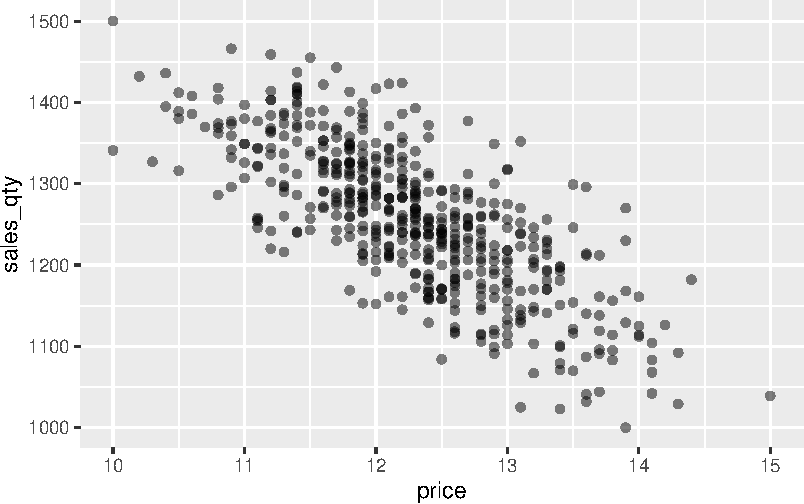
\includegraphics[keepaspectratio]{modules/01-data-visualization/point-plots_files/figure-pdf/fig-price-demand-1.pdf}}

}

\caption{\label{fig-price-demand}Price demand relationship}

\end{figure}%

Figure~\ref{fig-price-demand} shows the relationship between
\emph{price} and \emph{sales\_qty}.

\begin{tcolorbox}[enhanced jigsaw, colback=white, leftrule=.75mm, toprule=.15mm, bottomtitle=1mm, breakable, coltitle=black, toptitle=1mm, title={Quick Check}, opacitybacktitle=0.6, colbacktitle=quarto-callout-note-color!10!white, arc=.35mm, left=2mm, colframe=quarto-callout-note-color-frame, titlerule=0mm, rightrule=.15mm, bottomrule=.15mm, opacityback=0]

Figure~\ref{fig-price-demand} which variable appears on the x-axis and
which one on the y-axis?

\end{tcolorbox}

\begin{tcolorbox}[enhanced jigsaw, colback=white, leftrule=.75mm, toprule=.15mm, bottomtitle=1mm, breakable, coltitle=black, toptitle=1mm, title={Suggested answer}, opacitybacktitle=0.6, colbacktitle=quarto-callout-note-color!10!white, arc=.35mm, left=2mm, colframe=quarto-callout-note-color-frame, titlerule=0mm, rightrule=.15mm, bottomrule=.15mm, opacityback=0]

x-axis: \emph{price} y-axis: \emph{sales\_qty}

\end{tcolorbox}

\begin{tcolorbox}[enhanced jigsaw, colback=white, leftrule=.75mm, toprule=.15mm, bottomtitle=1mm, breakable, coltitle=black, toptitle=1mm, title={Quick Check}, opacitybacktitle=0.6, colbacktitle=quarto-callout-note-color!10!white, arc=.35mm, left=2mm, colframe=quarto-callout-note-color-frame, titlerule=0mm, rightrule=.15mm, bottomrule=.15mm, opacityback=0]

What two numbers determine the location of a point in
Figure~\ref{fig-price-demand}?

\end{tcolorbox}

\begin{tcolorbox}[enhanced jigsaw, colback=white, leftrule=.75mm, toprule=.15mm, bottomtitle=1mm, breakable, coltitle=black, toptitle=1mm, title={Suggested answer}, opacitybacktitle=0.6, colbacktitle=quarto-callout-note-color!10!white, arc=.35mm, left=2mm, colframe=quarto-callout-note-color-frame, titlerule=0mm, rightrule=.15mm, bottomrule=.15mm, opacityback=0]

Its x-value (\emph{price}) and its y-value (\emph{sales\_qty})

\end{tcolorbox}

\begin{tcolorbox}[enhanced jigsaw, colback=white, leftrule=.75mm, toprule=.15mm, bottomtitle=1mm, breakable, coltitle=black, toptitle=1mm, title={Quick Check}, opacitybacktitle=0.6, colbacktitle=quarto-callout-note-color!10!white, arc=.35mm, left=2mm, colframe=quarto-callout-note-color-frame, titlerule=0mm, rightrule=.15mm, bottomrule=.15mm, opacityback=0]

If a point is at x = 14 and y = 1100, how does that relate to the data
frame on which the plot was based?

\end{tcolorbox}

\begin{tcolorbox}[enhanced jigsaw, colback=white, leftrule=.75mm, toprule=.15mm, bottomtitle=1mm, breakable, coltitle=black, toptitle=1mm, title={Suggested answer}, opacitybacktitle=0.6, colbacktitle=quarto-callout-note-color!10!white, arc=.35mm, left=2mm, colframe=quarto-callout-note-color-frame, titlerule=0mm, rightrule=.15mm, bottomrule=.15mm, opacityback=0]

There is an observation (row in the \emph{price\_demand} data frame)
where the price was 14 and the monthly sales quantity is 1100.

\end{tcolorbox}

Note the following about the plot:

\begin{itemize}
\tightlist
\item
  The plot has two axes -- the x-axis along the width and the y-axis
  along the height.
\item
  The plot shows the values of price on the x-axis and the values of
  sales\_qty on the y-axis.
\item
  If you take any single point on the plot, you can drop a vertical line
  from the point to the x-axis and the point where it intersects the
  x-axis is the \emph{price} corresponding to the point.
\item
  Similarly, if you draw a horizontal line from the point to intersect
  the y-axis, you get the \emph{sales\_qty} corresponding to that point.
\item
  Each point of the plot corresponds to one row of the data frame. So
  how many points are on the plot? 500, since the data frame has 500
  rows.
\item
  Thus given a point on the plot, we should be able to identify a
  corresponding row of the data frame
\item
  Given a row of the data frame, we should be able to identify a
  corresponding point on the plot.
\end{itemize}

\begin{tcolorbox}[enhanced jigsaw, colback=white, leftrule=.75mm, toprule=.15mm, bottomtitle=1mm, breakable, coltitle=black, toptitle=1mm, title={Quick Check}, opacitybacktitle=0.6, colbacktitle=quarto-callout-note-color!10!white, arc=.35mm, left=2mm, colframe=quarto-callout-note-color-frame, titlerule=0mm, rightrule=.15mm, bottomrule=.15mm, opacityback=0]

True or False: Two different rows can produce the exact same point.

\end{tcolorbox}

\begin{tcolorbox}[enhanced jigsaw, colback=white, leftrule=.75mm, toprule=.15mm, bottomtitle=1mm, breakable, coltitle=black, toptitle=1mm, title={Suggested answer}, opacitybacktitle=0.6, colbacktitle=quarto-callout-note-color!10!white, arc=.35mm, left=2mm, colframe=quarto-callout-note-color-frame, titlerule=0mm, rightrule=.15mm, bottomrule=.15mm, opacityback=0]

True. If two rows have identical price and sales\_qty, they would
overlap at the same location.

\end{tcolorbox}

\begin{tcolorbox}[enhanced jigsaw, colback=white, leftrule=.75mm, toprule=.15mm, bottomtitle=1mm, breakable, coltitle=black, toptitle=1mm, title={Quick Check}, opacitybacktitle=0.6, colbacktitle=quarto-callout-note-color!10!white, arc=.35mm, left=2mm, colframe=quarto-callout-note-color-frame, titlerule=0mm, rightrule=.15mm, bottomrule=.15mm, opacityback=0]

If you see an extreme point far above the rest, what does that imply
about its row in the data frame?

\end{tcolorbox}

\begin{tcolorbox}[enhanced jigsaw, colback=white, leftrule=.75mm, toprule=.15mm, bottomtitle=1mm, breakable, coltitle=black, toptitle=1mm, title={Suggested answer}, opacitybacktitle=0.6, colbacktitle=quarto-callout-note-color!10!white, arc=.35mm, left=2mm, colframe=quarto-callout-note-color-frame, titlerule=0mm, rightrule=.15mm, bottomrule=.15mm, opacityback=0]

The row on which the point is based has an unusually high sales\_qty
value relative to the others (for its price).

\end{tcolorbox}

\begin{tcolorbox}[enhanced jigsaw, colback=white, leftrule=.75mm, toprule=.15mm, bottomtitle=1mm, breakable, coltitle=black, toptitle=1mm, title={Quick Check}, opacitybacktitle=0.6, colbacktitle=quarto-callout-note-color!10!white, arc=.35mm, left=2mm, colframe=quarto-callout-note-color-frame, titlerule=0mm, rightrule=.15mm, bottomrule=.15mm, opacityback=0]

Why might it be hard to identify the exact row for a point just from the
plot?

\end{tcolorbox}

\begin{tcolorbox}[enhanced jigsaw, colback=white, leftrule=.75mm, toprule=.15mm, bottomtitle=1mm, breakable, coltitle=black, toptitle=1mm, title={Suggested answer}, opacitybacktitle=0.6, colbacktitle=quarto-callout-note-color!10!white, arc=.35mm, left=2mm, colframe=quarto-callout-note-color-frame, titlerule=0mm, rightrule=.15mm, bottomrule=.15mm, opacityback=0]

Many points can be close together or overlapping, and it can be hard to
poinpoint exactly where the center of a plotted point falls.

\end{tcolorbox}

\subsection{Finding the point corresponding to a row of the data
frame}\label{finding-the-point-corresponding-to-a-row-of-the-data-frame}

Let us now try to find the point on the plot corresponding to the first
row in Figure~\ref{fig-price-demand}.

The first row of the data frame has \emph{price = 11.8} and
\emph{sales\_qty = 1260}. Therefore, we can find the point by drawing a
vertical line from 11.8 on the x-axis to intersect a horizontal line
from 1260 on the y-axis. Figure~\ref{fig-first-row-price-demand-on-plot}
illustrates this. We have highlighted the point by enlarging it.

\begin{figure}

\centering{

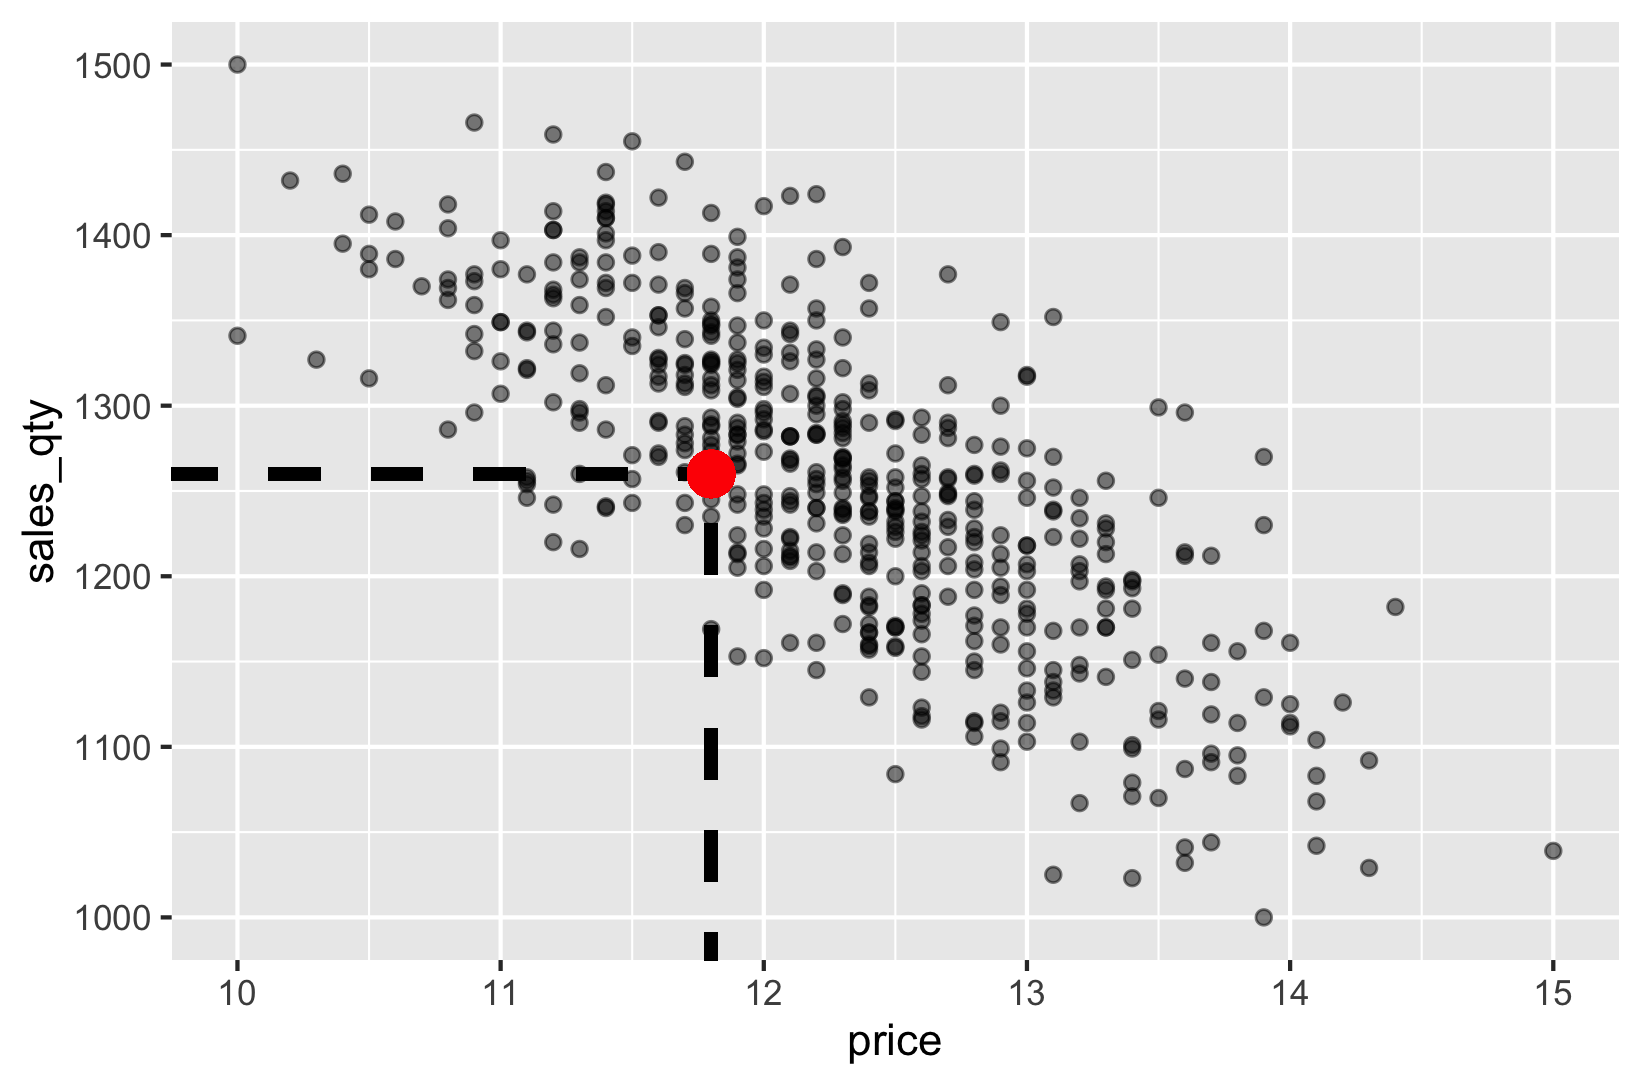
\includegraphics[width=0.7\linewidth,height=\textheight,keepaspectratio]{modules/01-data-visualization/../../images/fig-first-row-price-demand-on-plot.png}

}

\caption{\label{fig-first-row-price-demand-on-plot}Finding the first row
of the \emph{price\_demand} data frame on the plot: \emph{price = 11.8},
\emph{sales\_qty = 1260}}

\end{figure}%

\begin{tcolorbox}[enhanced jigsaw, colback=white, leftrule=.75mm, toprule=.15mm, bottomtitle=1mm, breakable, coltitle=black, toptitle=1mm, title={Quick Check}, opacitybacktitle=0.6, colbacktitle=quarto-callout-note-color!10!white, arc=.35mm, left=2mm, colframe=quarto-callout-note-color-frame, titlerule=0mm, rightrule=.15mm, bottomrule=.15mm, opacityback=0]

Suppose a row has \emph{price = 12.5} and \emph{sales\_qty} = 1200.
Describe how to locate its point on the plot.

\end{tcolorbox}

\begin{tcolorbox}[enhanced jigsaw, colback=white, leftrule=.75mm, toprule=.15mm, bottomtitle=1mm, breakable, coltitle=black, toptitle=1mm, title={Suggested answer}, opacitybacktitle=0.6, colbacktitle=quarto-callout-note-color!10!white, arc=.35mm, left=2mm, colframe=quarto-callout-note-color-frame, titlerule=0mm, rightrule=.15mm, bottomrule=.15mm, opacityback=0]

Find 12.5 on the x-axis, move up to where y is 1200, and mark the
intersection.

\end{tcolorbox}

\begin{tcolorbox}[enhanced jigsaw, colback=white, leftrule=.75mm, toprule=.15mm, bottomtitle=1mm, breakable, coltitle=black, toptitle=1mm, title={Quick Check}, opacitybacktitle=0.6, colbacktitle=quarto-callout-note-color!10!white, arc=.35mm, left=2mm, colframe=quarto-callout-note-color-frame, titlerule=0mm, rightrule=.15mm, bottomrule=.15mm, opacityback=0]

If you draw a vertical line at \emph{price} = 13, you will cut through
several points. What is common to all of these?

\end{tcolorbox}

\begin{tcolorbox}[enhanced jigsaw, colback=white, leftrule=.75mm, toprule=.15mm, bottomtitle=1mm, breakable, coltitle=black, toptitle=1mm, title={Suggested answer}, opacitybacktitle=0.6, colbacktitle=quarto-callout-note-color!10!white, arc=.35mm, left=2mm, colframe=quarto-callout-note-color-frame, titlerule=0mm, rightrule=.15mm, bottomrule=.15mm, opacityback=0]

They all correspond to rows that have \emph{price} = 13.

\end{tcolorbox}

Similarly, let us locate the point corresponding to row 11 (\emph{price
= 13.3}, \emph{sales\_qty = 1170}).

following the same approach we arrive at
Figure~\ref{fig-eleventh-row-price-demand-on-plot}.

\begin{figure}

\centering{

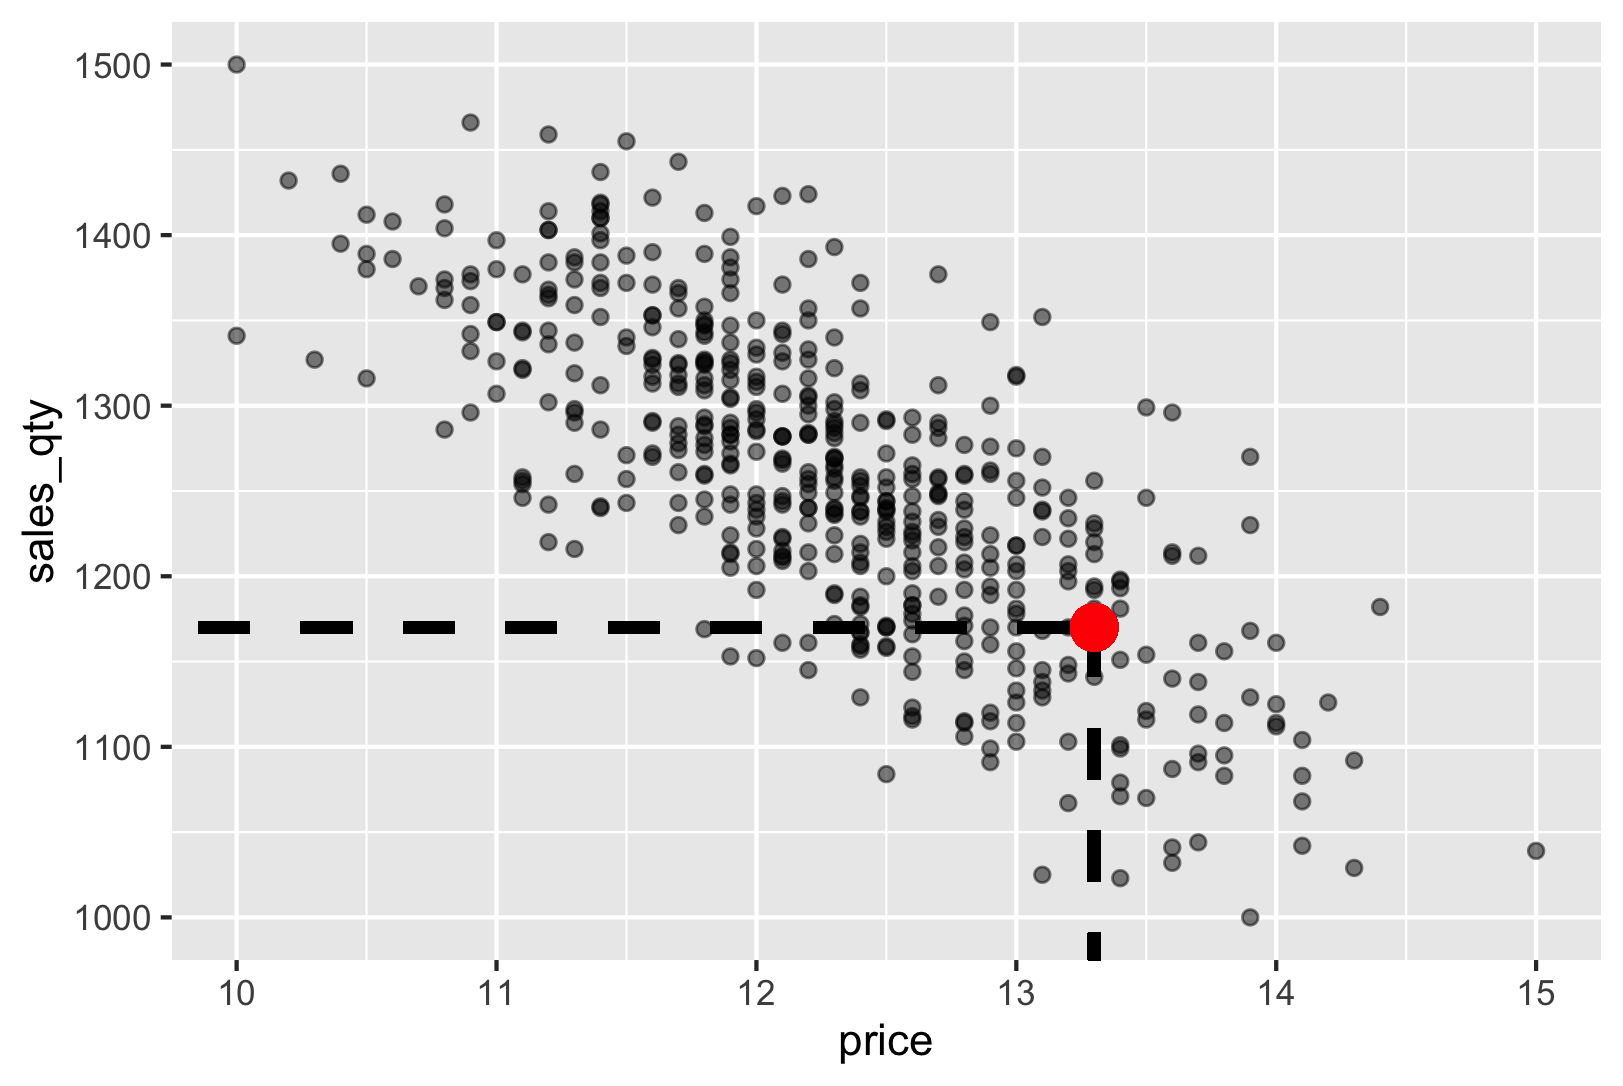
\includegraphics[width=0.7\linewidth,height=\textheight,keepaspectratio]{modules/01-data-visualization/../../images/fig-eleventh-row-price-demand-on-plot.png}

}

\caption{\label{fig-eleventh-row-price-demand-on-plot}Finding the
eleventh row of the \emph{price\_demand} data frame on the plot:
\emph{price = 13.3}, \emph{sales\_qty = 1170}}

\end{figure}%

\subsection{\texorpdfstring{Finding the \emph{price} and
\emph{sales\_qty} corresponding to a point on the
plot}{Finding the price and sales\_qty corresponding to a point on the plot}}\label{finding-the-price-and-sales_qty-corresponding-to-a-point-on-the-plot}

We can reverse the above process to find the variable values (and hence
the actual row) corresponding to a point on the plot. We will simply
drop a vertical line from the point down to the x-axis to get the
\emph{price} and draw a horizontal line from the point to the y-axis to
determine the \emph{sales\_qty}. The figure will look similar to the
prior two figures.

\subsection{Dissecting the code}\label{dissecting-the-code}

Figure~\ref{fig-first-point-plot-code} decodes the various elements of
the code that we used to generate out first point plot in
Figure~\ref{fig-price-demand}. We see that we pass the data frame
\emph{price\_demand} to the \emph{point\_plot} function through the
\emph{pipe} operator. We add the tilde expression for the plot as an
additional argument.

Figure~\ref{fig-basic-tilde-expression} shows us that the
\emph{point\_plot} function maps the variable on the left of the tilde
operator to the y-axis of the plot and maps the variable to the right of
the tilde expression to the x-axis of the plot.

\begin{figure}

\centering{

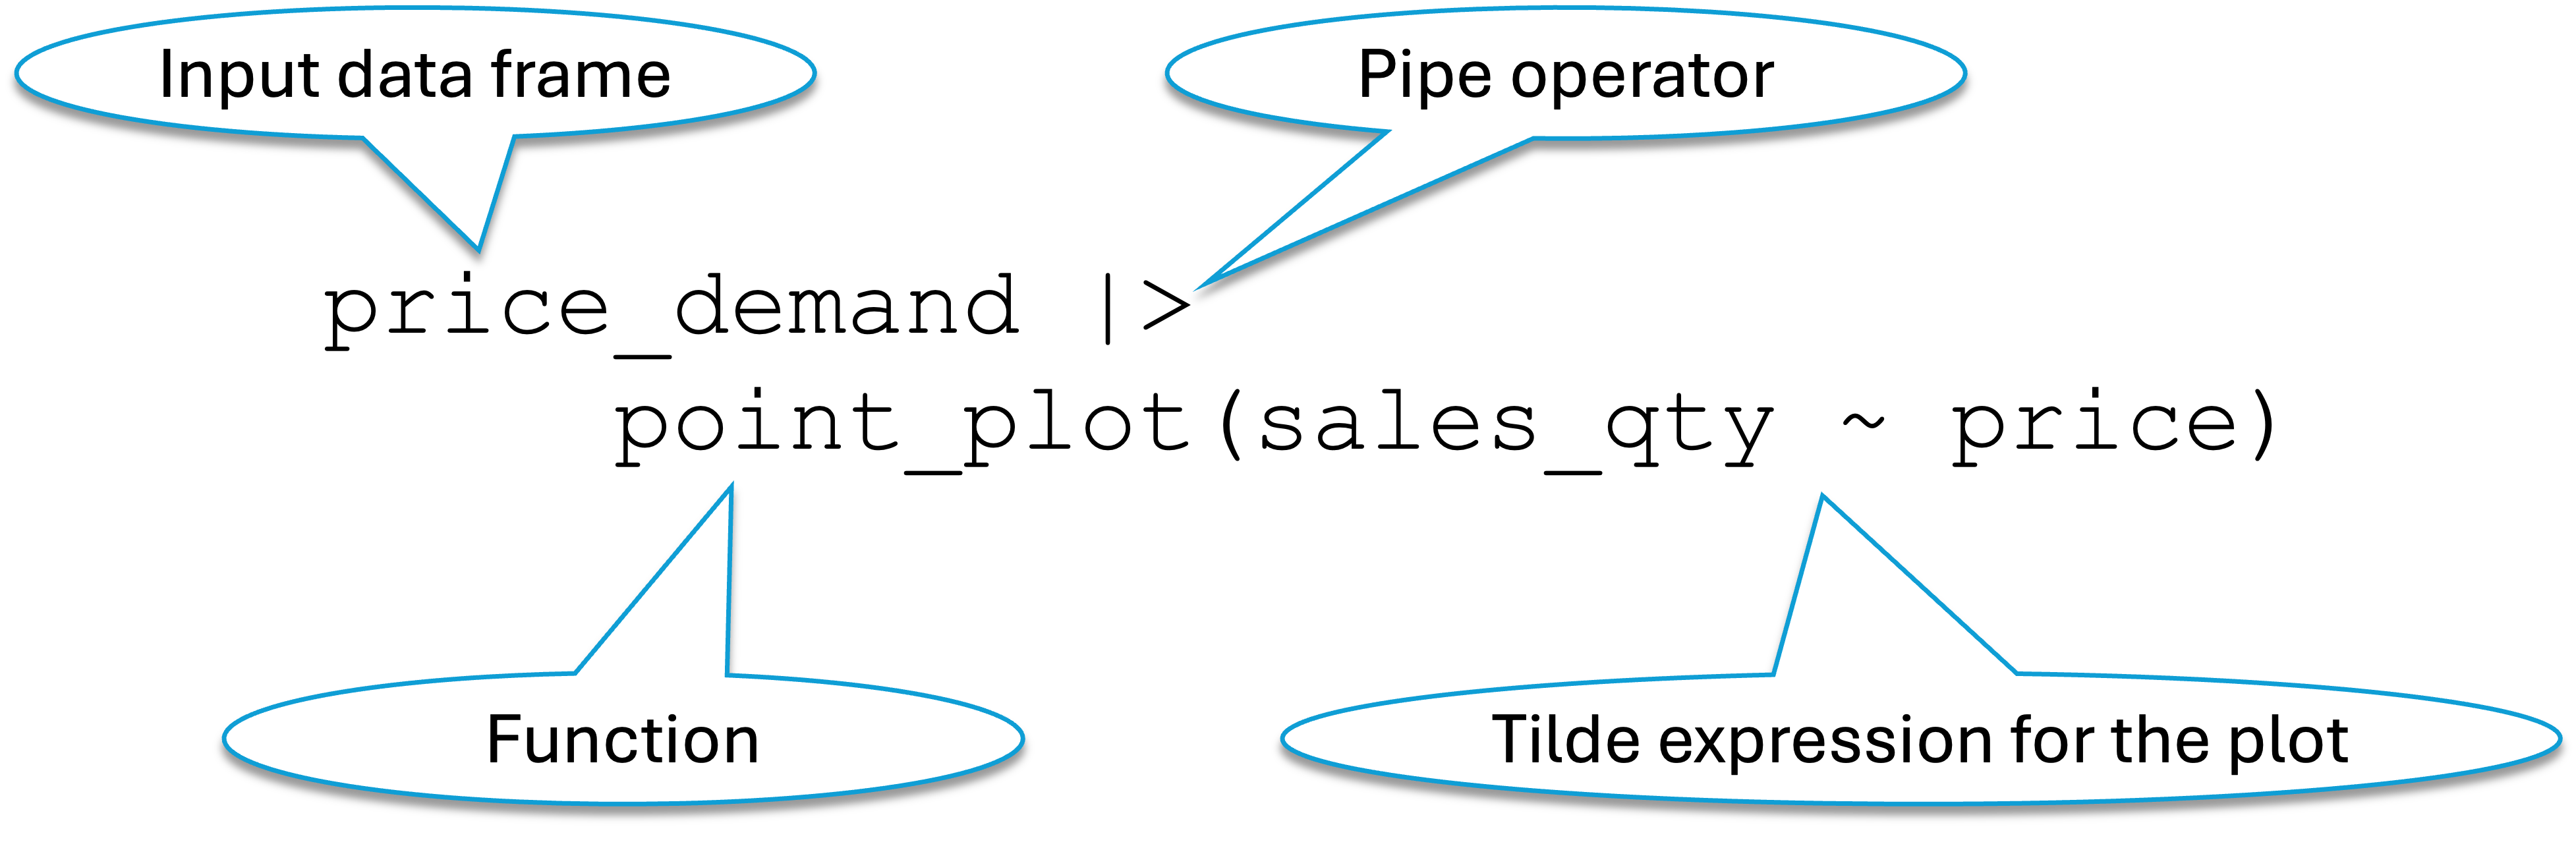
\includegraphics[width=0.7\linewidth,height=\textheight,keepaspectratio]{modules/01-data-visualization/../../images/fig-first-point-plot-code.png}

}

\caption{\label{fig-first-point-plot-code}Passing the
\emph{price\_demand} data frame as argument to the \emph{point\_plot}
function through the pipe operator}

\end{figure}%

\begin{figure}

\centering{

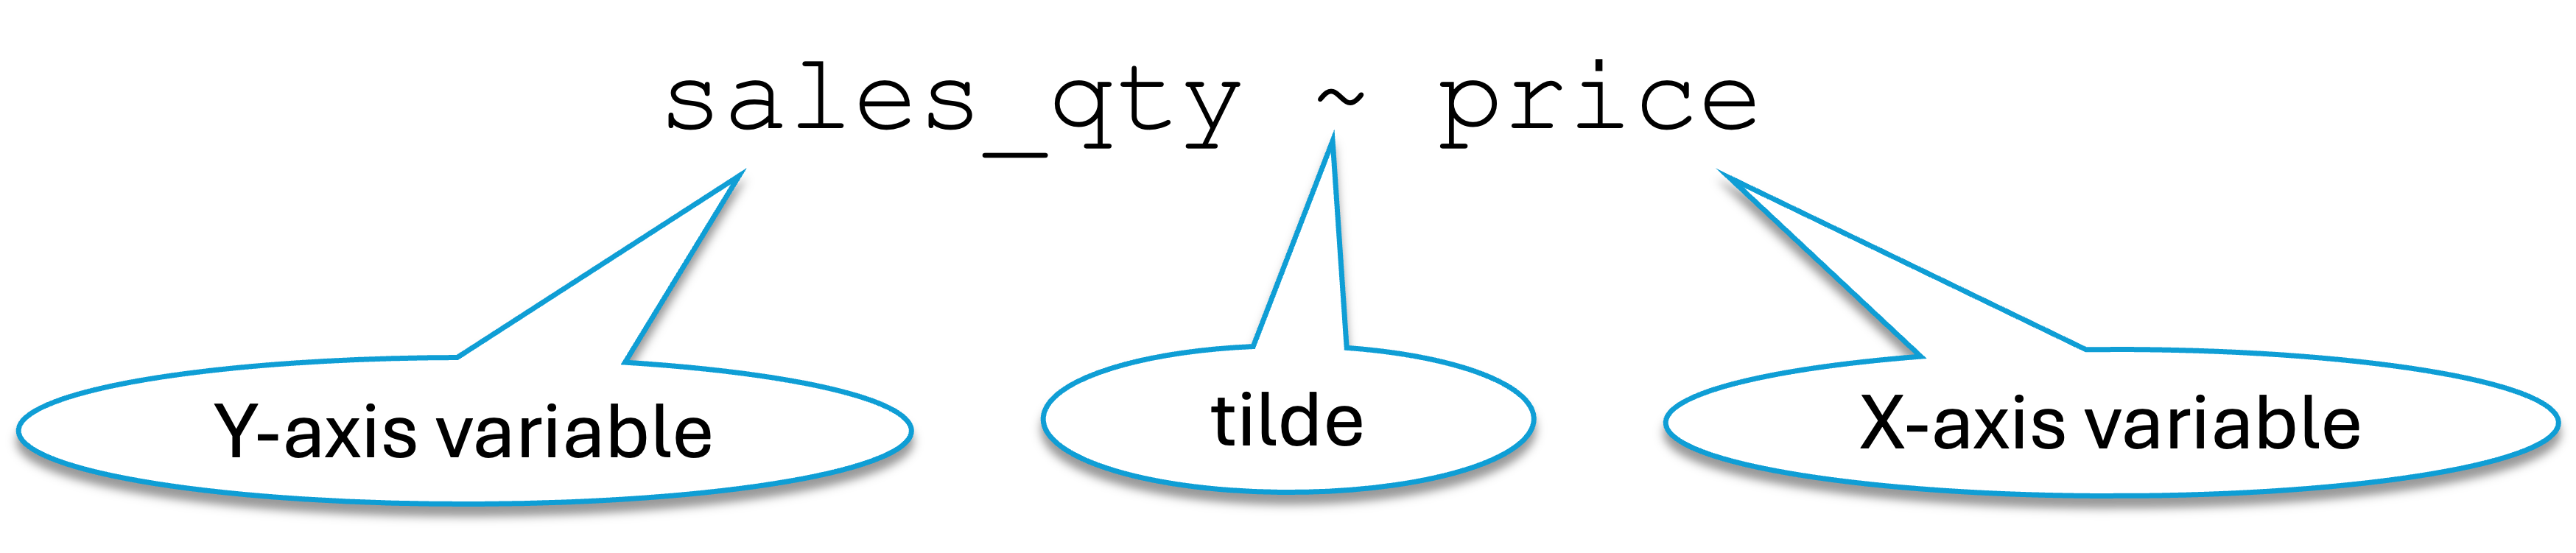
\includegraphics[width=0.7\linewidth,height=\textheight,keepaspectratio]{modules/01-data-visualization/../../images/fig-basic-tilde-expression.png}

}

\caption{\label{fig-basic-tilde-expression}Using a tilde expression to
map variables to the axes}

\end{figure}%

\begin{tcolorbox}[enhanced jigsaw, colback=white, leftrule=.75mm, toprule=.15mm, bottomtitle=1mm, breakable, coltitle=black, toptitle=1mm, title={Quick Check}, opacitybacktitle=0.6, colbacktitle=quarto-callout-note-color!10!white, arc=.35mm, left=2mm, colframe=quarto-callout-note-color-frame, titlerule=0mm, rightrule=.15mm, bottomrule=.15mm, opacityback=0]

In a y \textasciitilde{} x formula for point\_plot, what does the tilde
mean operationally?

\end{tcolorbox}

\begin{tcolorbox}[enhanced jigsaw, colback=white, leftrule=.75mm, toprule=.15mm, bottomtitle=1mm, breakable, coltitle=black, toptitle=1mm, title={Suggested answer}, opacitybacktitle=0.6, colbacktitle=quarto-callout-note-color!10!white, arc=.35mm, left=2mm, colframe=quarto-callout-note-color-frame, titlerule=0mm, rightrule=.15mm, bottomrule=.15mm, opacityback=0]

It separates the y-variable (left) from the x-variable (right), mapping
them to the plot axes.

\end{tcolorbox}

\begin{tcolorbox}[enhanced jigsaw, colback=white, leftrule=.75mm, toprule=.15mm, bottomtitle=1mm, breakable, coltitle=black, toptitle=1mm, title={Quick Check}, opacitybacktitle=0.6, colbacktitle=quarto-callout-note-color!10!white, arc=.35mm, left=2mm, colframe=quarto-callout-note-color-frame, titlerule=0mm, rightrule=.15mm, bottomrule=.15mm, opacityback=0]

Write the formula you would use to plot weekly\_sales\_k on the y-axis
against advertising\_spend\_k on the x-axis. Write only the tilde
expression.

\end{tcolorbox}

\begin{tcolorbox}[enhanced jigsaw, colback=white, leftrule=.75mm, toprule=.15mm, bottomtitle=1mm, breakable, coltitle=black, toptitle=1mm, title={Suggested answer}, opacitybacktitle=0.6, colbacktitle=quarto-callout-note-color!10!white, arc=.35mm, left=2mm, colframe=quarto-callout-note-color-frame, titlerule=0mm, rightrule=.15mm, bottomrule=.15mm, opacityback=0]

weekly\_sales\_k \textasciitilde{} advertising\_spend\_k

\end{tcolorbox}

\begin{tcolorbox}[enhanced jigsaw, colback=white, leftrule=.75mm, toprule=.15mm, bottomtitle=1mm, breakable, coltitle=black, toptitle=1mm, title={Quick Check}, opacitybacktitle=0.6, colbacktitle=quarto-callout-note-color!10!white, arc=.35mm, left=2mm, colframe=quarto-callout-note-color-frame, titlerule=0mm, rightrule=.15mm, bottomrule=.15mm, opacityback=0]

If you accidentally write price \textasciitilde{} sales\_qty, what
changes in the appearance of the plot?

\end{tcolorbox}

\begin{tcolorbox}[enhanced jigsaw, colback=white, leftrule=.75mm, toprule=.15mm, bottomtitle=1mm, breakable, coltitle=black, toptitle=1mm, title={Suggested answer}, opacitybacktitle=0.6, colbacktitle=quarto-callout-note-color!10!white, arc=.35mm, left=2mm, colframe=quarto-callout-note-color-frame, titlerule=0mm, rightrule=.15mm, bottomrule=.15mm, opacityback=0]

The axes swap: price becomes the y-axis and sales quantity becomes the
x-axis.

\end{tcolorbox}

\subsection{Interpreting the plot}\label{interpreting-the-plot}

Figure~\ref{fig-price-demand-2} repeats the plot of \emph{price} versus
\emph{sales\_qty}.

\begin{lstlisting}[language=R]
price_demand |> 
  point_plot(sales_qty ~ price)
\end{lstlisting}

\begin{figure}[H]

\centering{

\pandocbounded{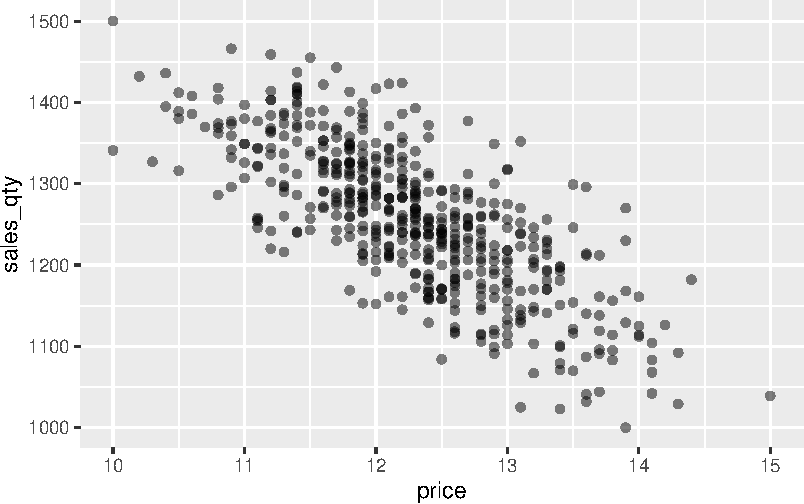
\includegraphics[keepaspectratio]{modules/01-data-visualization/point-plots_files/figure-pdf/fig-price-demand-2-1.pdf}}

}

\caption{\label{fig-price-demand-2}Price demand relationship (again)}

\end{figure}%

We can see a clear trend showing that, in general, higher prices
correspond to lower values of sales quantity.

To be sure, this is only a trend and not a strict rule. That is, given
any two points, we do not have a guarantee that the point with the
higher price will always have a lower sales quantity. However, this will
be true for most of the pairs of points.
Figure~\ref{fig-scatter-with-line-segments-1} illustrates this with some
randomly selected pairs of points. We see that most of the lines point
down and to the right -- meaning that for most pairs of points, the one
with higher \emph{price} has a lower \emph{sales\_qty}. However, we also
see a few examples where the opposite is true.

This is why we only calls this a \emph{trend} and not a strict rule
about the relationship between price and sales\_qty.

\begin{figure}

\centering{

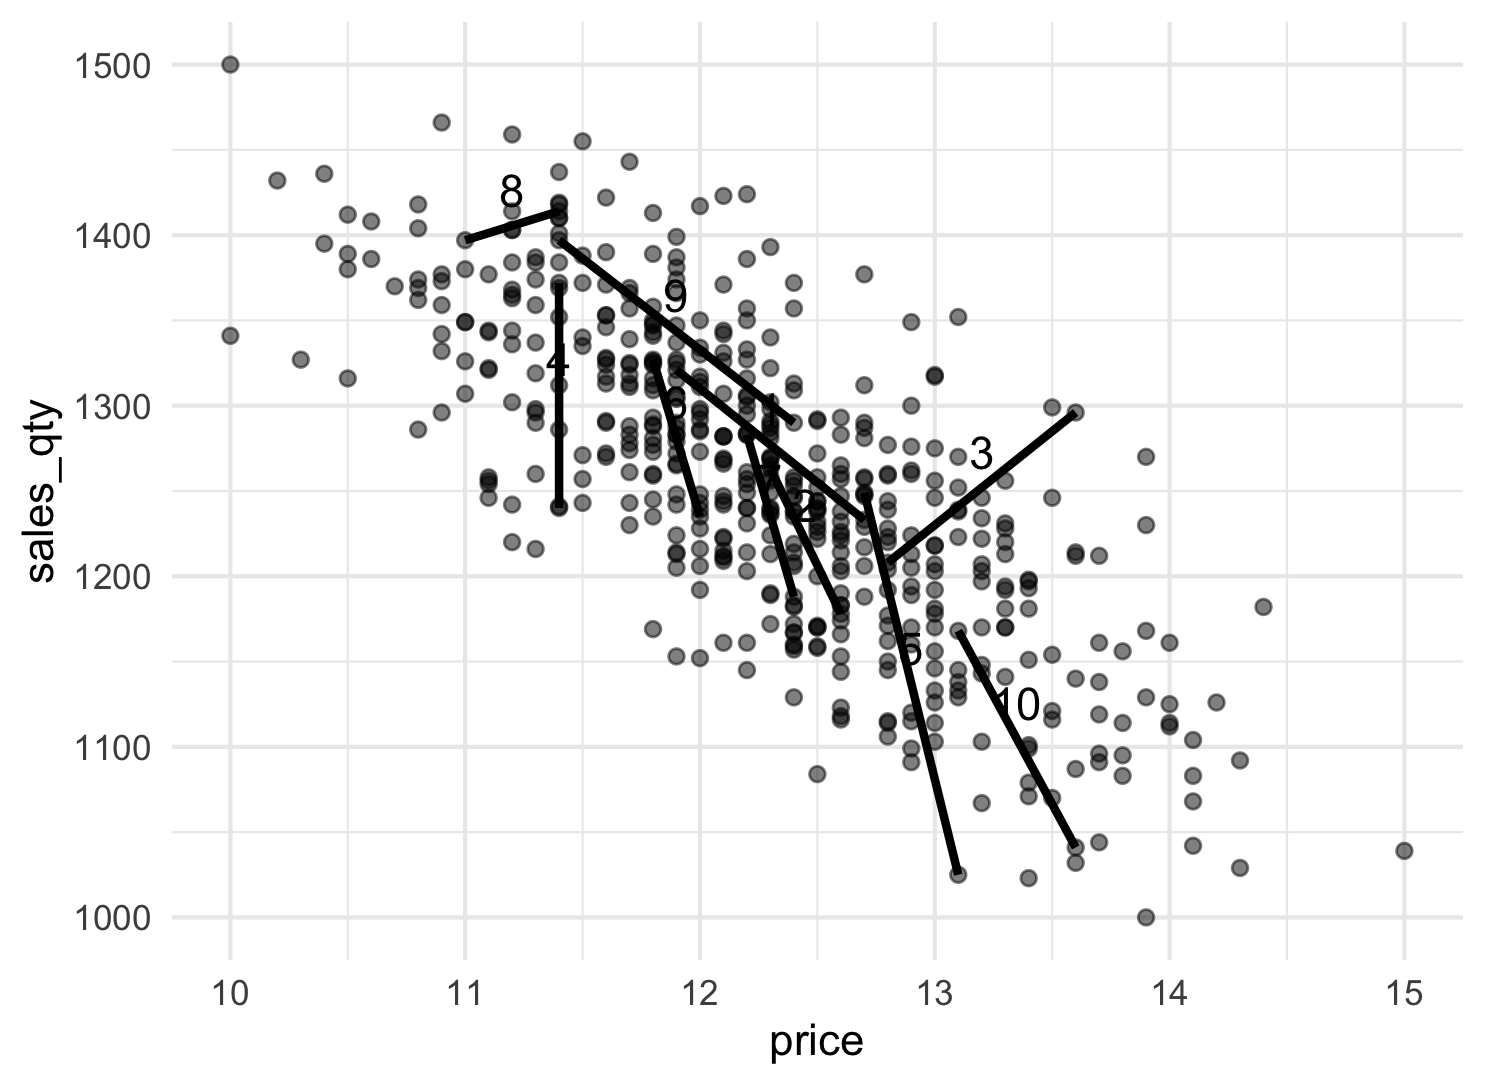
\includegraphics[width=0.7\linewidth,height=\textheight,keepaspectratio]{modules/01-data-visualization/../../images/fig-scatter-with-line-segments-1.png}

}

\caption{\label{fig-scatter-with-line-segments-1}Line segments
connecting some pairs of points showing that for most pairs of points
the point with higher price has lower sales\_qty}

\end{figure}%

\begin{tcolorbox}[enhanced jigsaw, colback=white, leftrule=.75mm, toprule=.15mm, bottomtitle=1mm, breakable, coltitle=black, toptitle=1mm, title={Quick Check}, opacitybacktitle=0.6, colbacktitle=quarto-callout-note-color!10!white, arc=.35mm, left=2mm, colframe=quarto-callout-note-color-frame, titlerule=0mm, rightrule=.15mm, bottomrule=.15mm, opacityback=0]

Describe a quick visual procedure to decide if the relationship is
positive, negative, or neither.

\end{tcolorbox}

\begin{tcolorbox}[enhanced jigsaw, colback=white, leftrule=.75mm, toprule=.15mm, bottomtitle=1mm, breakable, coltitle=black, toptitle=1mm, title={Suggested answer}, opacitybacktitle=0.6, colbacktitle=quarto-callout-note-color!10!white, arc=.35mm, left=2mm, colframe=quarto-callout-note-color-frame, titlerule=0mm, rightrule=.15mm, bottomrule=.15mm, opacityback=0]

Look at the overall slope of the cloud from left to right: up =
positive, down = negative, no slope = neither.

\end{tcolorbox}

\begin{tcolorbox}[enhanced jigsaw, colback=white, leftrule=.75mm, toprule=.15mm, bottomtitle=1mm, breakable, coltitle=black, toptitle=1mm, title={Quick Check}, opacitybacktitle=0.6, colbacktitle=quarto-callout-note-color!10!white, arc=.35mm, left=2mm, colframe=quarto-callout-note-color-frame, titlerule=0mm, rightrule=.15mm, bottomrule=.15mm, opacityback=0]

In the price vs sales plot, why do we call it a trend and not a rule?

\end{tcolorbox}

\begin{tcolorbox}[enhanced jigsaw, colback=white, leftrule=.75mm, toprule=.15mm, bottomtitle=1mm, breakable, coltitle=black, toptitle=1mm, title={Suggested answer}, opacitybacktitle=0.6, colbacktitle=quarto-callout-note-color!10!white, arc=.35mm, left=2mm, colframe=quarto-callout-note-color-frame, titlerule=0mm, rightrule=.15mm, bottomrule=.15mm, opacityback=0]

Because points vary; higher price usually means lower sales, but not for
every single pair of observations.

\end{tcolorbox}

\begin{tcolorbox}[enhanced jigsaw, colback=white, leftrule=.75mm, toprule=.15mm, bottomtitle=1mm, breakable, coltitle=black, toptitle=1mm, title={Quick Check}, opacitybacktitle=0.6, colbacktitle=quarto-callout-note-color!10!white, arc=.35mm, left=2mm, colframe=quarto-callout-note-color-frame, titlerule=0mm, rightrule=.15mm, bottomrule=.15mm, opacityback=0]

What would a ``no linear relationship'' scatterplot look like?

\end{tcolorbox}

\begin{tcolorbox}[enhanced jigsaw, colback=white, leftrule=.75mm, toprule=.15mm, bottomtitle=1mm, breakable, coltitle=black, toptitle=1mm, title={Suggested answer}, opacitybacktitle=0.6, colbacktitle=quarto-callout-note-color!10!white, arc=.35mm, left=2mm, colframe=quarto-callout-note-color-frame, titlerule=0mm, rightrule=.15mm, bottomrule=.15mm, opacityback=0]

A roughly pattern less cloud with no clear upward or downward slope.

\end{tcolorbox}

\subsection{Positive and negative
relationships}\label{positive-and-negative-relationships}

In general, when we discuss the relationship between two numerical
variables, if the general trend is that higher values of one correspond
to higher values of the other, then we have a positive relationship. On
the other hand, is higher values of one variable correspond to lower
values of the other then we have a negative relationship.

What kind of relationship does Figure~\ref{fig-price-demand-2} show --
positive or negative?

You got it right if you said \emph{negative} -- higher values of
\emph{price} correspond to lower values of \emph{sales\_qty}.

Figure~\ref{fig-advertising-sales-channel-1} shows two positively
correlated variables. Here, higher values of one variable are generally
related to higher values of the other. We used the
\emph{advertising\_sales\_channel} data frame for this plot.

\begin{lstlisting}[language=R]
advertising_sales_channel |> 
  point_plot(weekly_sales_k ~ advertising_spend_k)
\end{lstlisting}

\begin{figure}[H]

\centering{

\pandocbounded{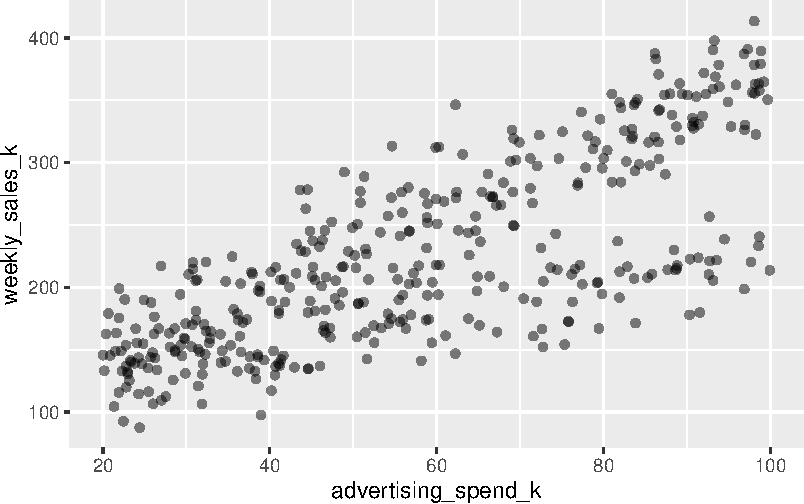
\includegraphics[keepaspectratio]{modules/01-data-visualization/point-plots_files/figure-pdf/fig-advertising-sales-channel-1-1.pdf}}

}

\caption{\label{fig-advertising-sales-channel-1}Weekly sales and
advertising spend have a positive relationship -- higher advertising
generally has higher weekly sales}

\end{figure}%

The data frame \emph{returns\_dpo} contains hypothetical data on various
firms' daily stock returns and the number of days they take to pay their
suppliers. Figure~\ref{fig-returns-dpo-1} shows the relationship between
these variables. We cannot spot any trend. Higher or lower values of one
variable do not indicate higher or lower values of the other. Hence
there is neither a positive relationship nor a negative one.

\begin{lstlisting}[language=R]
returns_dpo |> 
  point_plot(daily_return ~ dpo)
\end{lstlisting}

\begin{figure}[H]

\centering{

\pandocbounded{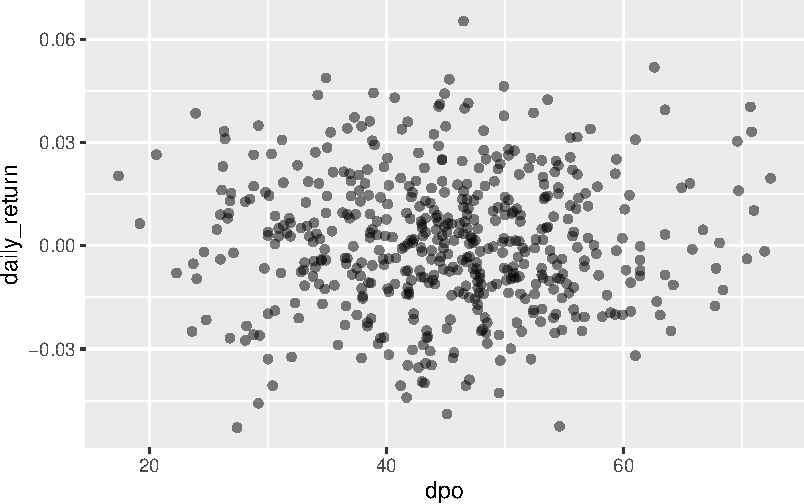
\includegraphics[keepaspectratio]{modules/01-data-visualization/point-plots_files/figure-pdf/fig-returns-dpo-1-1.pdf}}

}

\caption{\label{fig-returns-dpo-1}Days payment outstanding (dpo) does
not have a relationship to the daily stock return}

\end{figure}%

\textbf{How to decide visually if there's a relationship}

Imagine the point cloud as a blob

\emph{Ask:} does it slope up, slope down, or neither? \emph{Ask:} tight
blob or wide blob?

\begin{tcolorbox}[enhanced jigsaw, colback=white, leftrule=.75mm, toprule=.15mm, bottomtitle=1mm, breakable, coltitle=black, toptitle=1mm, title={Quick Check}, opacitybacktitle=0.6, colbacktitle=quarto-callout-note-color!10!white, arc=.35mm, left=2mm, colframe=quarto-callout-note-color-frame, titlerule=0mm, rightrule=.15mm, bottomrule=.15mm, opacityback=0]

Label each plot as positive, negative, or no clear relationship: (a)
price vs sales\_qty, (b) advertising vs weekly sales, (c) dpo vs daily
return.

\end{tcolorbox}

\begin{tcolorbox}[enhanced jigsaw, colback=white, leftrule=.75mm, toprule=.15mm, bottomtitle=1mm, breakable, coltitle=black, toptitle=1mm, title={Suggested answer}, opacitybacktitle=0.6, colbacktitle=quarto-callout-note-color!10!white, arc=.35mm, left=2mm, colframe=quarto-callout-note-color-frame, titlerule=0mm, rightrule=.15mm, bottomrule=.15mm, opacityback=0]

\begin{enumerate}
\def\labelenumi{(\alph{enumi})}
\tightlist
\item
  negative, (b) positive, (c) no clear relationship.
\end{enumerate}

\end{tcolorbox}

\begin{tcolorbox}[enhanced jigsaw, colback=white, leftrule=.75mm, toprule=.15mm, bottomtitle=1mm, breakable, coltitle=black, toptitle=1mm, title={Quick Check}, opacitybacktitle=0.6, colbacktitle=quarto-callout-note-color!10!white, arc=.35mm, left=2mm, colframe=quarto-callout-note-color-frame, titlerule=0mm, rightrule=.15mm, bottomrule=.15mm, opacityback=0]

If a scatterplot has a positive relationship, what do you expect most
left-to-right line segments between random pairs of points to do?

\end{tcolorbox}

\begin{tcolorbox}[enhanced jigsaw, colback=white, leftrule=.75mm, toprule=.15mm, bottomtitle=1mm, breakable, coltitle=black, toptitle=1mm, title={Suggested answer}, opacitybacktitle=0.6, colbacktitle=quarto-callout-note-color!10!white, arc=.35mm, left=2mm, colframe=quarto-callout-note-color-frame, titlerule=0mm, rightrule=.15mm, bottomrule=.15mm, opacityback=0]

Point up and to the right.

\end{tcolorbox}

\subsection{Putting a number on the relationship: The correlation
coefficient}\label{putting-a-number-on-the-relationship-the-correlation-coefficient}

Thus far, we have been talking about relationships between variables.
Exact sciences like mathematics and statistics like to be precise and
assign numbers where possible. Statistics commonly uses the
\emph{correlation coefficient} to quantify the relationship between two
numerical variables. This section just introduces the \emph{correlation
coefficient} and shows you how to compute it using R. We will get into
the mechanics of the actual computation later in the book.

The correlation coefficient can take a value between -1 and +1. A value
of 0 signifies \emph{no linear relationship}. -1 signifies a perfect
negative correlation and +1 signifies a perfect positive correlation. We
discuss these ideas below.

\begin{tcolorbox}[enhanced jigsaw, colback=white, leftrule=.75mm, toprule=.15mm, bottomtitle=1mm, breakable, coltitle=black, toptitle=1mm, title={Quick Check}, opacitybacktitle=0.6, colbacktitle=quarto-callout-note-color!10!white, arc=.35mm, left=2mm, colframe=quarto-callout-note-color-frame, titlerule=0mm, rightrule=.15mm, bottomrule=.15mm, opacityback=0]

What does the sign of the correlation coefficient tell you?

\end{tcolorbox}

\begin{tcolorbox}[enhanced jigsaw, colback=white, leftrule=.75mm, toprule=.15mm, bottomtitle=1mm, breakable, coltitle=black, toptitle=1mm, title={Suggested answer}, opacitybacktitle=0.6, colbacktitle=quarto-callout-note-color!10!white, arc=.35mm, left=2mm, colframe=quarto-callout-note-color-frame, titlerule=0mm, rightrule=.15mm, bottomrule=.15mm, opacityback=0]

Direction: positive means upward trend (as we go to the right); negative
means downward trend (as we go to the right).

\end{tcolorbox}

\begin{tcolorbox}[enhanced jigsaw, colback=white, leftrule=.75mm, toprule=.15mm, bottomtitle=1mm, breakable, coltitle=black, toptitle=1mm, title={Quick Check}, opacitybacktitle=0.6, colbacktitle=quarto-callout-note-color!10!white, arc=.35mm, left=2mm, colframe=quarto-callout-note-color-frame, titlerule=0mm, rightrule=.15mm, bottomrule=.15mm, opacityback=0]

What does the magnitude (absolute value, that is, value without the
sign) tell you?

\end{tcolorbox}

\begin{tcolorbox}[enhanced jigsaw, colback=white, leftrule=.75mm, toprule=.15mm, bottomtitle=1mm, breakable, coltitle=black, toptitle=1mm, title={Suggested answer}, opacitybacktitle=0.6, colbacktitle=quarto-callout-note-color!10!white, arc=.35mm, left=2mm, colframe=quarto-callout-note-color-frame, titlerule=0mm, rightrule=.15mm, bottomrule=.15mm, opacityback=0]

Strength of the linear pattern: closer to 1 means points lie closer to a
straight line.

\end{tcolorbox}

\begin{tcolorbox}[enhanced jigsaw, colback=white, leftrule=.75mm, toprule=.15mm, bottomtitle=1mm, breakable, coltitle=black, toptitle=1mm, title={Quick Check}, opacitybacktitle=0.6, colbacktitle=quarto-callout-note-color!10!white, arc=.35mm, left=2mm, colframe=quarto-callout-note-color-frame, titlerule=0mm, rightrule=.15mm, bottomrule=.15mm, opacityback=0]

True or False: r = 0 proves there is no relationship of any kind.

\end{tcolorbox}

\begin{tcolorbox}[enhanced jigsaw, colback=white, leftrule=.75mm, toprule=.15mm, bottomtitle=1mm, breakable, coltitle=black, toptitle=1mm, title={Suggested answer}, opacitybacktitle=0.6, colbacktitle=quarto-callout-note-color!10!white, arc=.35mm, left=2mm, colframe=quarto-callout-note-color-frame, titlerule=0mm, rightrule=.15mm, bottomrule=.15mm, opacityback=0]

False. It indicates no \emph{linear relationship}; there could still be
a curved or other non-linear relationship. We show an example later.

\end{tcolorbox}

We look at some examples now. Revisiting the \emph{price\_demand} data
frame, let us use R to compute the correlation coefficient between the
variables \emph{price} and \emph{sales\_qty}.

\begin{lstlisting}[language=R]
price_demand |> 
  summarize(price_sales_qty_correlation = cor(price, sales_qty))
\end{lstlisting}

\begin{lstlisting}
# A tibble: 1 x 1
  price_sales_qty_correlation
                        <dbl>
1                      -0.752
\end{lstlisting}

We are computing a summary and hence use the \emph{summarize} function
(see Section~\ref{sec-summarize-function}). Since the summary we are
computing now is the correlation coefficient, we use the \emph{cor}
function within the \emph{summarize} function. We have chosen to call
the computed result \emph{price\_sales\_qty\_correlation}. We could have
named it anything we wanted, but chose the sensible approach of giving
it a meaningful name.

Figure~\ref{fig-price-demand} had already shown us the negative
relationship between \emph{price} and \emph{sales\_qty}. The correlation
confirms it, \ldots{} and makes it more precise.

\begin{tcolorbox}[enhanced jigsaw, colback=white, leftrule=.75mm, toprule=.15mm, bottomtitle=1mm, breakable, coltitle=black, toptitle=1mm, title={Quick Check}, opacitybacktitle=0.6, colbacktitle=quarto-callout-note-color!10!white, arc=.35mm, left=2mm, colframe=quarto-callout-note-color-frame, titlerule=0mm, rightrule=.15mm, bottomrule=.15mm, opacityback=0]

If the scatterplot slopes down and the correlation is -0.75, do these
agree?

\end{tcolorbox}

\begin{tcolorbox}[enhanced jigsaw, colback=white, leftrule=.75mm, toprule=.15mm, bottomtitle=1mm, breakable, coltitle=black, toptitle=1mm, title={Suggested answer}, opacitybacktitle=0.6, colbacktitle=quarto-callout-note-color!10!white, arc=.35mm, left=2mm, colframe=quarto-callout-note-color-frame, titlerule=0mm, rightrule=.15mm, bottomrule=.15mm, opacityback=0]

Yes. Negative sign matches the downward trend; 0.75 magnitude suggests a
fairly strong linear relationship.

\end{tcolorbox}

\begin{tcolorbox}[enhanced jigsaw, colback=white, leftrule=.75mm, toprule=.15mm, bottomtitle=1mm, breakable, coltitle=black, toptitle=1mm, title={Quick Check}, opacitybacktitle=0.6, colbacktitle=quarto-callout-note-color!10!white, arc=.35mm, left=2mm, colframe=quarto-callout-note-color-frame, titlerule=0mm, rightrule=.15mm, bottomrule=.15mm, opacityback=0]

If two variables have correlation coefficient close to +1, what will the
scatterplot look like?

\end{tcolorbox}

\begin{tcolorbox}[enhanced jigsaw, colback=white, leftrule=.75mm, toprule=.15mm, bottomtitle=1mm, breakable, coltitle=black, toptitle=1mm, title={Suggested answer}, opacitybacktitle=0.6, colbacktitle=quarto-callout-note-color!10!white, arc=.35mm, left=2mm, colframe=quarto-callout-note-color-frame, titlerule=0mm, rightrule=.15mm, bottomrule=.15mm, opacityback=0]

Points clustered tightly around a line sloping upward.

\end{tcolorbox}

Let us compute the correlation coefficient between advertising spend and
the weekly sales from the \emph{advertising\_sales\_channel} data frame.
From Figure~\ref{fig-advertising-sales-channel-1} we saw that these two
variables are positively related. Let us see what the correlation
coefficient says.

\begin{lstlisting}[language=R]
advertising_sales_channel |> 
  summarize(ad_sales_corr = cor(advertising_spend_k, weekly_sales_k))
\end{lstlisting}

\begin{lstlisting}
# A tibble: 1 x 1
  ad_sales_corr
          <dbl>
1         0.760
\end{lstlisting}

Sure enough, we see a positive correlation coefficient.

\subsection{Perfect correlation}\label{perfect-correlation}

Consider Figure~\ref{fig-price-demand-3} showing strong, but imperfect,
correlation.

\begin{lstlisting}[language=R]
price_demand |> 
  point_plot(sales_qty ~ price)
\end{lstlisting}

\begin{figure}[H]

\centering{

\pandocbounded{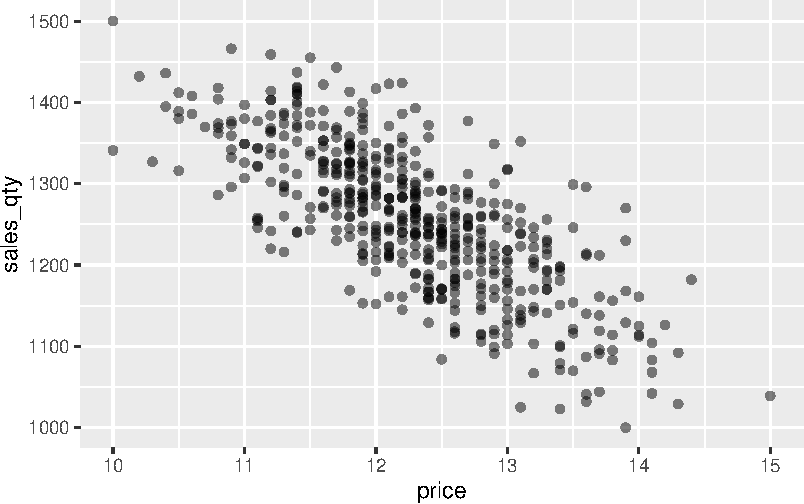
\includegraphics[keepaspectratio]{modules/01-data-visualization/point-plots_files/figure-pdf/fig-price-demand-3-1.pdf}}

}

\caption{\label{fig-price-demand-3}Price and sales\_qty are not
perfectly correlated -- correlation coefficient is -0.75}

\end{figure}%

We have already established that \emph{price} and \emph{sales\_qty} are
negatively related. That is, there is a general pattern that higher
values of \emph{price} have lower values of \emph{sales\_qty}.

In Figure~\ref{fig-price-demand-3}, if we look only at the points
corresponding to a particular value of \emph{price}, say 13, the points
along this vertical line range from approximately 1100 to 1320. That is,
given a value of \emph{price}, we cannot be sure about the exact value
of the corresponding value of \emph{sales\_qty}. However, knowing
\emph{price} does give us some idea about \emph{sale\_qty}. This shows
relationship, but not perfect correlation.

When the correlation coefficient is +1 or -1, we have perfect
correlation. In this case, knowing the value of one variable enables us
to precisely know the value of the other variable as well. This happens
when all the points lie on a straight line instead of being dispersed as
a cloud as in Figure~\ref{fig-price-demand-3}.

\begin{figure}

\centering{

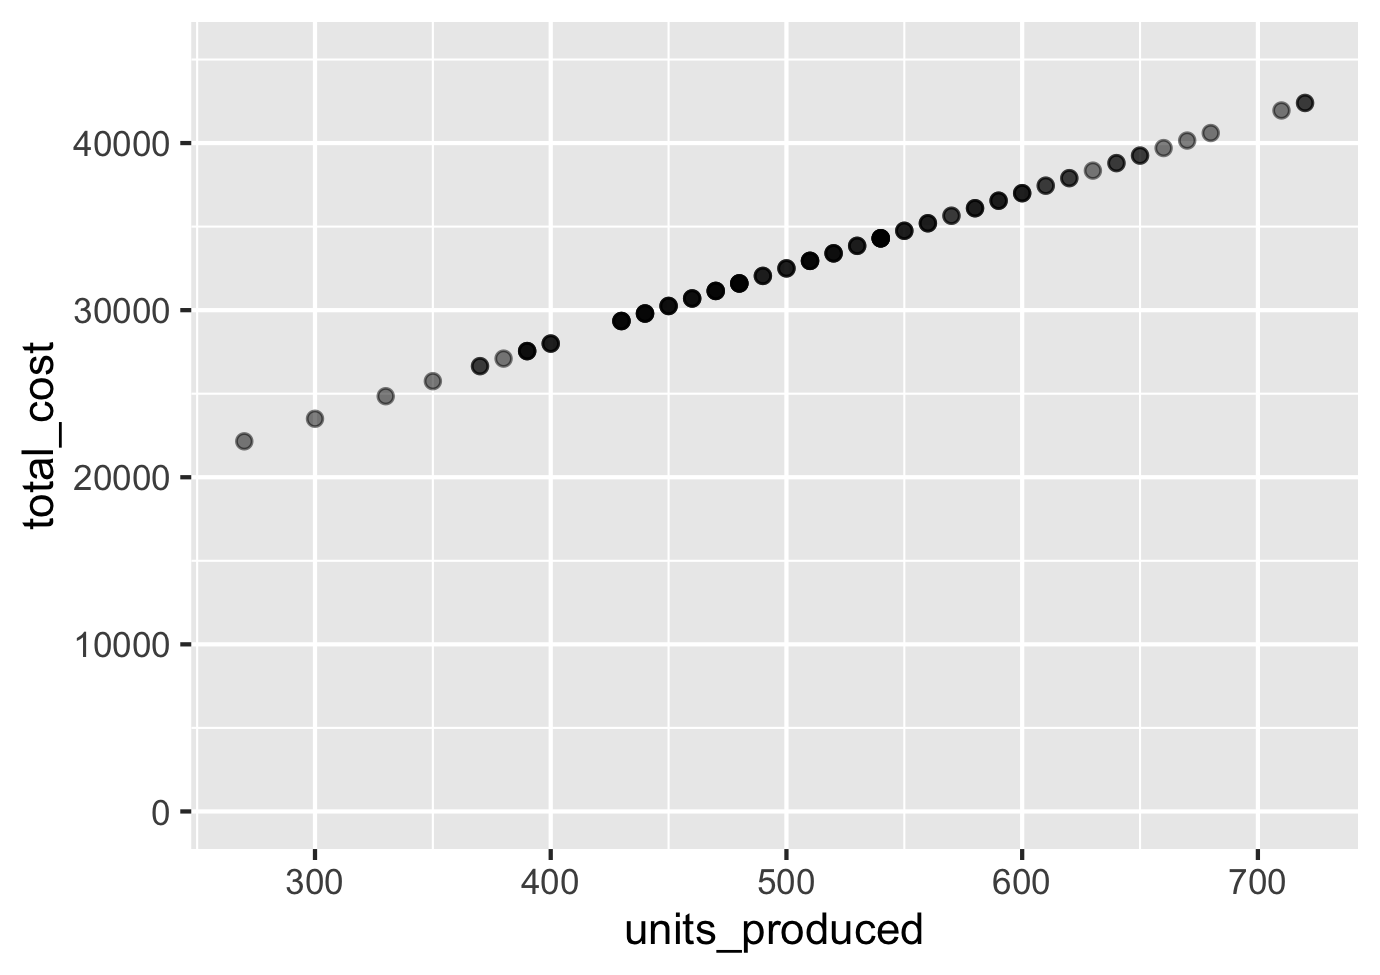
\includegraphics[width=0.7\linewidth,height=\textheight,keepaspectratio]{modules/01-data-visualization/../../images/fig-production-cost-units-produced.png}

}

\caption{\label{fig-production-cost-units-produced}Perfect correlation
arises when all the points lie perfectly on a straight line -- the
variables in this plot have a correlation coefficient of +1}

\end{figure}%

Figure~\ref{fig-production-cost-units-produced} shows a situation when
all points lie on a perfect straight line. In this case, given a value
for one variable, we can determine exactly the value of the other. We
can determine it visually or by plugging the value of the known variable
into the following equation and calculating the value of the other
variable.

\begin{lstlisting}[language=R]
total_cost = 10000 + 45*units_produced
\end{lstlisting}

In Figure~\ref{fig-production-cost-units-produced} the line slopes
upward as it goes from left to right. When the line on which all points
fall slopes down as it goes right, the correlation is still perfect, but
the line slopes down as it goes to the right and so we have a
correlation coefficient of -1.

\subsection{How the point cloud looks for various correlation
coefficients}\label{how-the-point-cloud-looks-for-various-correlation-coefficients}

Figure~\ref{fig-various-corr-coeffs} shows the point plots for various
values of correlation coefficients between -1 and +1.

\begin{figure}

\centering{

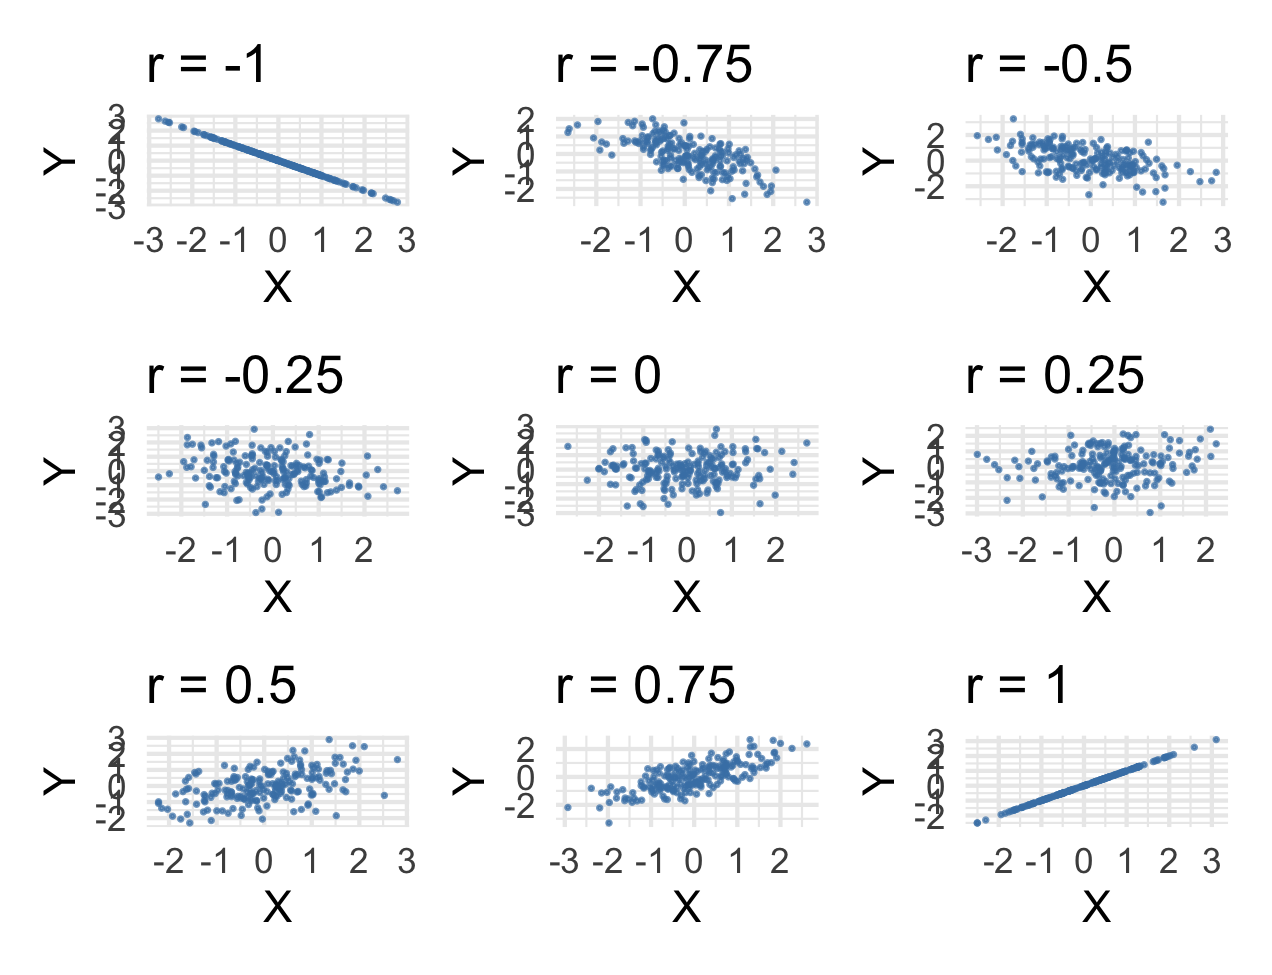
\includegraphics[width=0.7\linewidth,height=\textheight,keepaspectratio]{modules/01-data-visualization/../../images/fig-various-corr-coeffs.png}

}

\caption{\label{fig-various-corr-coeffs}Point plots for various
correlation-coefficients (r)}

\end{figure}%

You can see the following: - in the plot with correlation coefficient =
-1 (r = -1), the points align perfectly on a straight line \emph{sloping
downwards} as the x values increase - at +1 they align perfectly on a
line \emph{sloping upwards} as the x values increase - as the
coefficient goes from -1 to 0, the points get more scattered away from
perfect alignment on a straight line until at 0 there is no pattern
whatsoever - as the correlation coefficient increases from 0 to +1, we
see that the tendency to align on a straight line increases until
perfect alignment at r = 1.

\begin{tcolorbox}[enhanced jigsaw, colback=white, leftrule=.75mm, toprule=.15mm, bottomtitle=1mm, breakable, coltitle=black, toptitle=1mm, title=\textcolor{quarto-callout-important-color}{\faExclamation}\hspace{0.5em}{Magnitude and sign of the correlation coefficient}, opacitybacktitle=0.6, colbacktitle=quarto-callout-important-color!10!white, arc=.35mm, left=2mm, colframe=quarto-callout-important-color-frame, titlerule=0mm, rightrule=.15mm, bottomrule=.15mm, opacityback=0]

\textbf{Sign:} Direction (positive/negative)

\textbf{Magnitude:} Tightness around a line (near 0 = no linear pattern;
near ±1 = points nearly on a line)

\end{tcolorbox}

\begin{tcolorbox}[enhanced jigsaw, colback=white, leftrule=.75mm, toprule=.15mm, bottomtitle=1mm, breakable, coltitle=black, toptitle=1mm, title={Quick Check}, opacitybacktitle=0.6, colbacktitle=quarto-callout-note-color!10!white, arc=.35mm, left=2mm, colframe=quarto-callout-note-color-frame, titlerule=0mm, rightrule=.15mm, bottomrule=.15mm, opacityback=0]

What does ``perfect correlation'' mean visually?

\end{tcolorbox}

\begin{tcolorbox}[enhanced jigsaw, colback=white, leftrule=.75mm, toprule=.15mm, bottomtitle=1mm, breakable, coltitle=black, toptitle=1mm, title={Suggested answer}, opacitybacktitle=0.6, colbacktitle=quarto-callout-note-color!10!white, arc=.35mm, left=2mm, colframe=quarto-callout-note-color-frame, titlerule=0mm, rightrule=.15mm, bottomrule=.15mm, opacityback=0]

All points lie exactly on a straight line.

\end{tcolorbox}

\begin{tcolorbox}[enhanced jigsaw, colback=white, leftrule=.75mm, toprule=.15mm, bottomtitle=1mm, breakable, coltitle=black, toptitle=1mm, title={Quick Check}, opacitybacktitle=0.6, colbacktitle=quarto-callout-note-color!10!white, arc=.35mm, left=2mm, colframe=quarto-callout-note-color-frame, titlerule=0mm, rightrule=.15mm, bottomrule=.15mm, opacityback=0]

If correlation is -1, does that mean the variables are weakly related?

\end{tcolorbox}

\begin{tcolorbox}[enhanced jigsaw, colback=white, leftrule=.75mm, toprule=.15mm, bottomtitle=1mm, breakable, coltitle=black, toptitle=1mm, title={Suggested answer}, opacitybacktitle=0.6, colbacktitle=quarto-callout-note-color!10!white, arc=.35mm, left=2mm, colframe=quarto-callout-note-color-frame, titlerule=0mm, rightrule=.15mm, bottomrule=.15mm, opacityback=0]

No.~It means perfectly related but in a negative (downward) direction.

\end{tcolorbox}

\begin{tcolorbox}[enhanced jigsaw, colback=white, leftrule=.75mm, toprule=.15mm, bottomtitle=1mm, breakable, coltitle=black, toptitle=1mm, title={Quick Check}, opacitybacktitle=0.6, colbacktitle=quarto-callout-note-color!10!white, arc=.35mm, left=2mm, colframe=quarto-callout-note-color-frame, titlerule=0mm, rightrule=.15mm, bottomrule=.15mm, opacityback=0]

As r moves from 0 toward 1, what changes visually?

\end{tcolorbox}

\begin{tcolorbox}[enhanced jigsaw, colback=white, leftrule=.75mm, toprule=.15mm, bottomtitle=1mm, breakable, coltitle=black, toptitle=1mm, title={Suggested answer}, opacitybacktitle=0.6, colbacktitle=quarto-callout-note-color!10!white, arc=.35mm, left=2mm, colframe=quarto-callout-note-color-frame, titlerule=0mm, rightrule=.15mm, bottomrule=.15mm, opacityback=0]

The point cloud becomes more tightly aligned around an upward-sloping
line.

\end{tcolorbox}

\begin{tcolorbox}[enhanced jigsaw, colback=white, leftrule=.75mm, toprule=.15mm, bottomtitle=1mm, breakable, coltitle=black, toptitle=1mm, title=\textcolor{quarto-callout-important-color}{\faExclamation}\hspace{0.5em}{Correlation vs.~\emph{Causation}}, opacitybacktitle=0.6, colbacktitle=quarto-callout-important-color!10!white, arc=.35mm, left=2mm, colframe=quarto-callout-important-color-frame, titlerule=0mm, rightrule=.15mm, bottomrule=.15mm, opacityback=0]

In Figure~\ref{fig-price-demand-3}, we can see that as \emph{price}
increases, \emph{sales\_qty} decreases. We have said that these two
variables are \emph{correlated}. From this alone, can we infer that
higher \emph{price} \textbf{caused} lower \emph{sales\_qty}?

We need to be very careful here. Figure~\ref{fig-price-demand-3} only
shows the \emph{correlation}. From that correlation alone we should
infer anything more. Specifically, we cannot infer that the \emph{price}
changes \textbf{cause} changes in \emph{sales}.

Of course, in the real world, we know that price increases generally
lead to drops in sales. But that knowledge lies outside of this data. It
is quite possible that, in this situation something else might be
playing a role. We just don't know from the data we are seeing.

Establishing \textbf{causation} is part of \emph{causal inference} which
uses other rigorous techniques to establish that something actually
caused something else. We do not go into causal inference in this
course.

\end{tcolorbox}

\section{Plotting a numerical variable against a categorical
one}\label{plotting-a-numerical-variable-against-a-categorical-one}

In this course, we will only assign a numerical variable to the y-axis.
Thus, if a plot has a categorical variable, it will only occupy the
x-axis.

Numerical and categorical variables differ in how they behave in plots.
In Figure~\ref{fig-advertising-sales-channel-1} we have the variable
\emph{advertising\_spend\_k} on the x-axis. Being a numerical variable,
it can potentially take on any value on the x-axis. On the other hand,
look at Figure~\ref{fig-bank-account-type-balance}.

\begin{figure}

\centering{

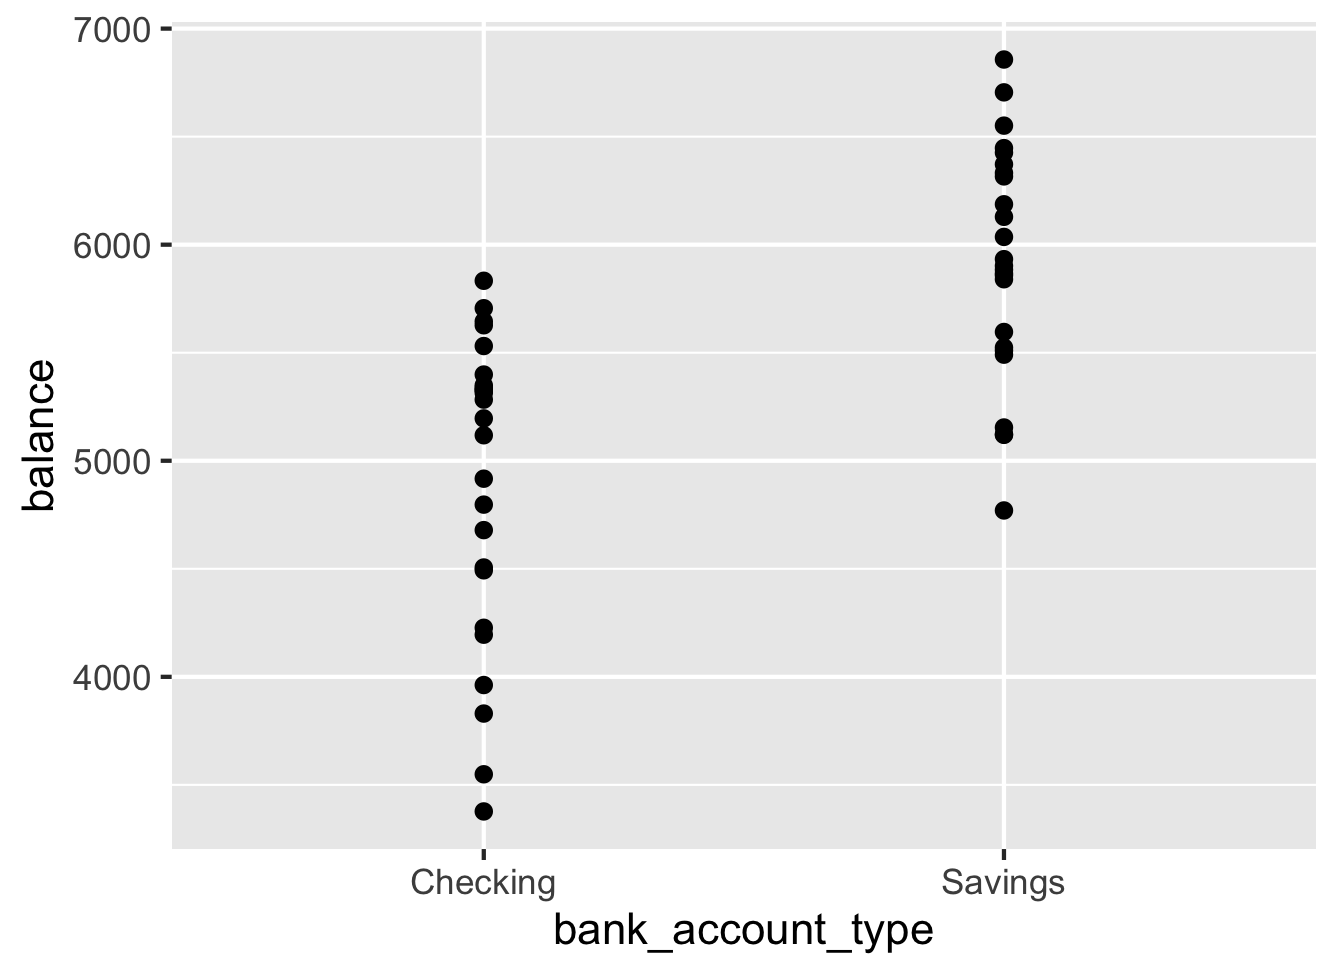
\includegraphics[width=0.7\linewidth,height=\textheight,keepaspectratio]{modules/01-data-visualization/../../images/fig-bank-account-type-balance.png}

}

\caption{\label{fig-bank-account-type-balance}Plotting a categorical
variable against a numerical one -- using the data frame
\emph{acct\_type\_balance} (not plotted using the \emph{point\_plot}
function)}

\end{figure}%

Here we have the variable \emph{bank\_account\_type} on the x-axis and
it can take on only one of two values \emph{``Checking''} and
\emph{``Savings''}. This is why each row falls at only one of two x
positions: one for \emph{Checking}, and one for \emph{Savings}. So
points stack vertically. If the row corresponds to a ``Checking''
account, it falls on the left stack of points and on the right stack
otherwise.

\subsection{A Caveat}\label{a-caveat}

Correlation measures the strength of a \emph{linear relationship}; a
curved pattern can have low correlation coefficient even if there is a
strong relationship.

Figure~\ref{fig-non-linear-strong-but-weak-corr-coeff} shows a strong
non-linear (loosely means ``not a \textbf{straight} line'')
relationship. The points align very close to a curved line. This has a
low correlation coefficient because if you try to run a straight line
through these points, no matter how hard you try, you cannot draw a line
that is even reasonably close to all points. The correlation coefficient
is -0.125 -- close to zero!

\begin{figure}

\centering{

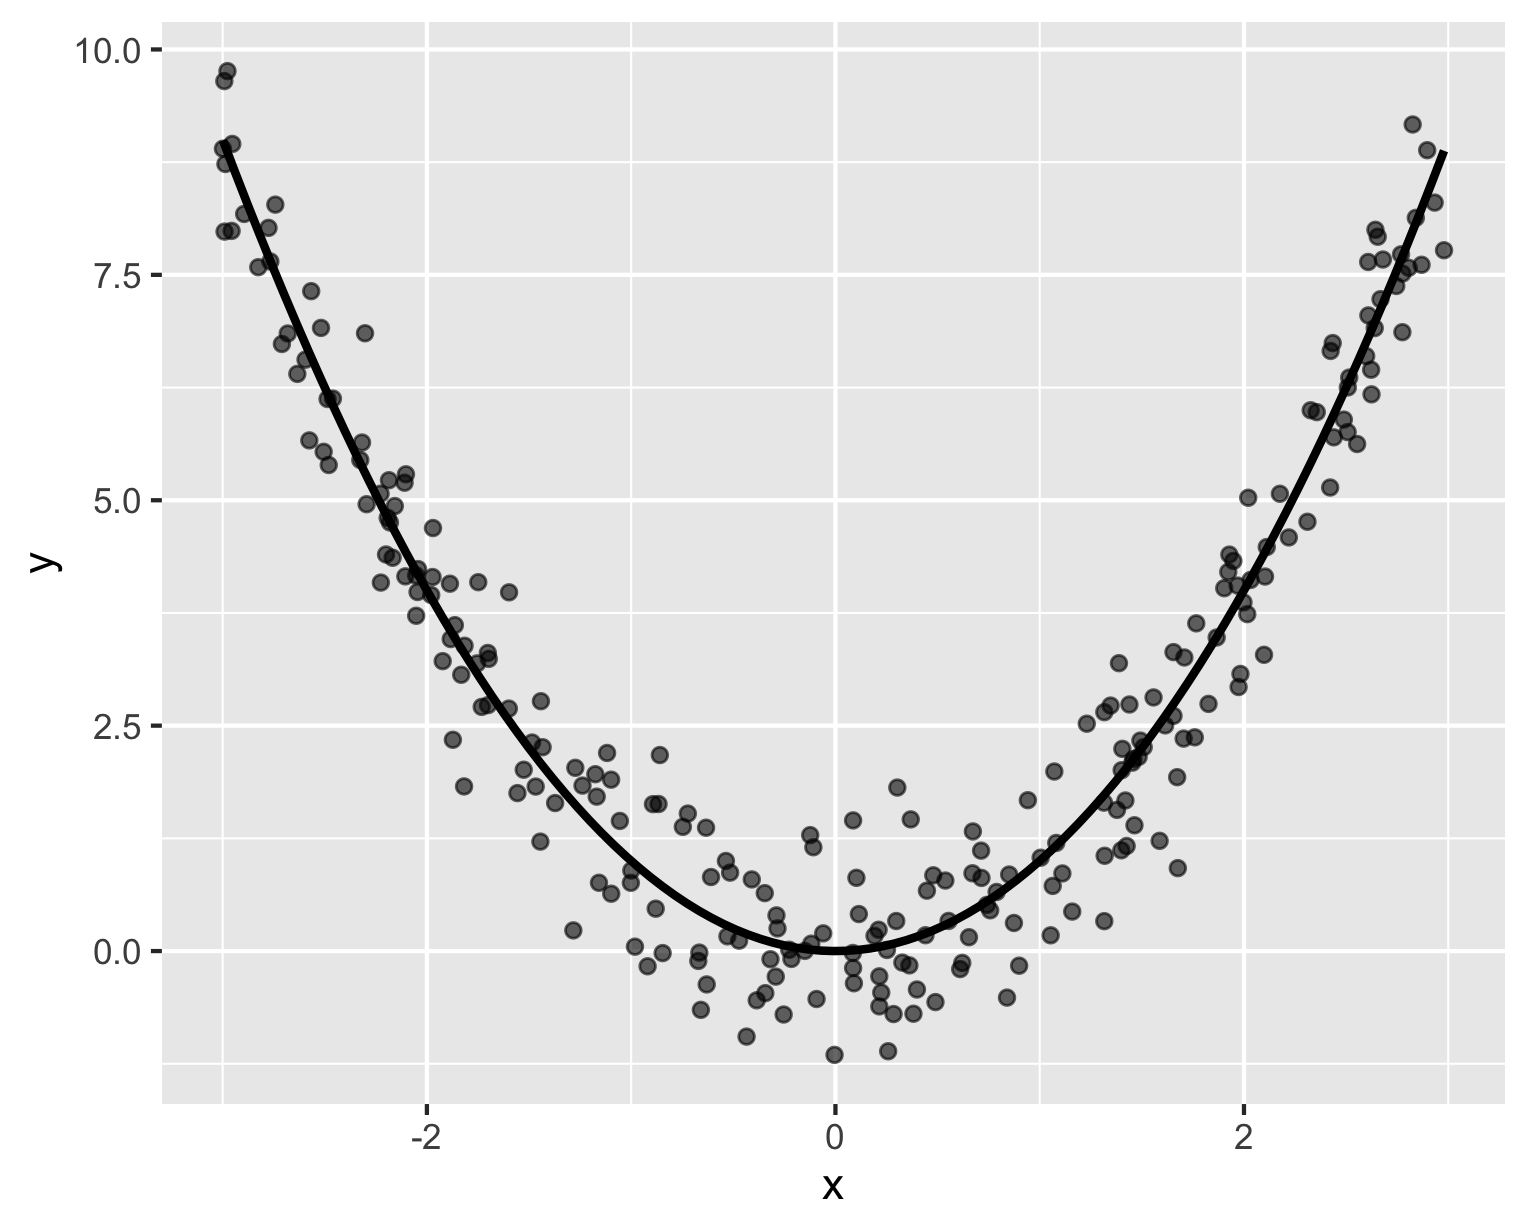
\includegraphics[width=0.7\linewidth,height=\textheight,keepaspectratio]{modules/01-data-visualization/../../images/fig-non-linear-strong-but-weak-corr-coeff.png}

}

\caption{\label{fig-non-linear-strong-but-weak-corr-coeff}Strong
non-linear relationship, but weak correlation coefficient}

\end{figure}%

\begin{tcolorbox}[enhanced jigsaw, colback=white, leftrule=.75mm, toprule=.15mm, bottomtitle=1mm, breakable, coltitle=black, toptitle=1mm, title={Quick Check}, opacitybacktitle=0.6, colbacktitle=quarto-callout-note-color!10!white, arc=.35mm, left=2mm, colframe=quarto-callout-note-color-frame, titlerule=0mm, rightrule=.15mm, bottomrule=.15mm, opacityback=0]

If \emph{bank\_account\_type} has two categories, how many distinct x
positions exist conceptually?

\end{tcolorbox}

\begin{tcolorbox}[enhanced jigsaw, colback=white, leftrule=.75mm, toprule=.15mm, bottomtitle=1mm, breakable, coltitle=black, toptitle=1mm, title={Suggested answer}, opacitybacktitle=0.6, colbacktitle=quarto-callout-note-color!10!white, arc=.35mm, left=2mm, colframe=quarto-callout-note-color-frame, titlerule=0mm, rightrule=.15mm, bottomrule=.15mm, opacityback=0]

Two: one for \emph{Checking} and one for \emph{Savings}.

\end{tcolorbox}

\begin{tcolorbox}[enhanced jigsaw, colback=white, leftrule=.75mm, toprule=.15mm, bottomtitle=1mm, breakable, coltitle=black, toptitle=1mm, title={Quick Check}, opacitybacktitle=0.6, colbacktitle=quarto-callout-note-color!10!white, arc=.35mm, left=2mm, colframe=quarto-callout-note-color-frame, titlerule=0mm, rightrule=.15mm, bottomrule=.15mm, opacityback=0]

Why do points form vertical ``stacks'' for each category?

\end{tcolorbox}

\begin{tcolorbox}[enhanced jigsaw, colback=white, leftrule=.75mm, toprule=.15mm, bottomtitle=1mm, breakable, coltitle=black, toptitle=1mm, title={Suggested answer}, opacitybacktitle=0.6, colbacktitle=quarto-callout-note-color!10!white, arc=.35mm, left=2mm, colframe=quarto-callout-note-color-frame, titlerule=0mm, rightrule=.15mm, bottomrule=.15mm, opacityback=0]

Because many rows share the same category (same x position) but differ
in balance (y).

\end{tcolorbox}

\subsection{\texorpdfstring{\emph{point\_plot} and
``jittering''}{point\_plot and ``jittering''}}\label{point_plot-and-jittering}

If we have two \emph{Checking} accounts with the same or very similar
balance, their points will overlap. Because of this over plotting, the
plot in Figure~\ref{fig-bank-account-type-balance} does not enable us to
look at all the points.

To overcome this problem, the \emph{point\_plot} function plots this
chart a bit differently. See
Figure~\ref{fig-account-type-balance-point-plot}.

\textbf{Important:} Jittering changes only the display position of
points to reduce overlap; it does not change the underlying data values

\begin{lstlisting}[language=R]
acct_type_balance |> 
  point_plot(balance ~ bank_account_type)
\end{lstlisting}

\begin{figure}[H]

\centering{

\pandocbounded{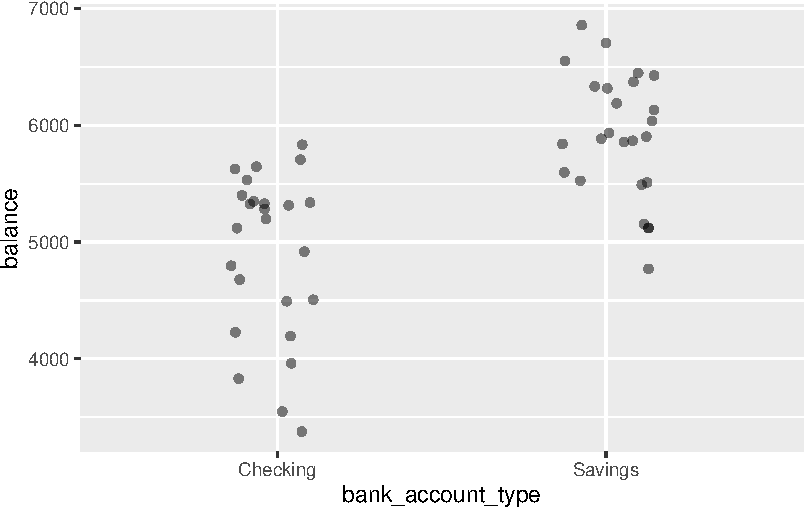
\includegraphics[keepaspectratio]{modules/01-data-visualization/point-plots_files/figure-pdf/fig-account-type-balance-point-plot-1.pdf}}

}

\caption{\label{fig-account-type-balance-point-plot}Plot of account type
against account bakance using the \emph{point\_plot function}: it
jitters the points along the x-axis to reduce overplotting}

\end{figure}%

To enable us to see the points more clearly, the \emph{point\_plot}
function randomly ``jitters'' the points along the x-axis to more
clearly separate points that might be over plotted or close together.

\begin{tcolorbox}[enhanced jigsaw, colback=white, leftrule=.75mm, toprule=.15mm, bottomtitle=1mm, breakable, coltitle=black, toptitle=1mm, title={Quick Check}, opacitybacktitle=0.6, colbacktitle=quarto-callout-note-color!10!white, arc=.35mm, left=2mm, colframe=quarto-callout-note-color-frame, titlerule=0mm, rightrule=.15mm, bottomrule=.15mm, opacityback=0]

What problem does jittering solve?

\end{tcolorbox}

\begin{tcolorbox}[enhanced jigsaw, colback=white, leftrule=.75mm, toprule=.15mm, bottomtitle=1mm, breakable, coltitle=black, toptitle=1mm, title={Suggested answer}, opacitybacktitle=0.6, colbacktitle=quarto-callout-note-color!10!white, arc=.35mm, left=2mm, colframe=quarto-callout-note-color-frame, titlerule=0mm, rightrule=.15mm, bottomrule=.15mm, opacityback=0]

Over plotting. Points hiding under other points.

\end{tcolorbox}

\begin{tcolorbox}[enhanced jigsaw, colback=white, leftrule=.75mm, toprule=.15mm, bottomtitle=1mm, breakable, coltitle=black, toptitle=1mm, title={Quick Check}, opacitybacktitle=0.6, colbacktitle=quarto-callout-note-color!10!white, arc=.35mm, left=2mm, colframe=quarto-callout-note-color-frame, titlerule=0mm, rightrule=.15mm, bottomrule=.15mm, opacityback=0]

Does jittering change the data?

\end{tcolorbox}

\begin{tcolorbox}[enhanced jigsaw, colback=white, leftrule=.75mm, toprule=.15mm, bottomtitle=1mm, breakable, coltitle=black, toptitle=1mm, title={Suggested answer}, opacitybacktitle=0.6, colbacktitle=quarto-callout-note-color!10!white, arc=.35mm, left=2mm, colframe=quarto-callout-note-color-frame, titlerule=0mm, rightrule=.15mm, bottomrule=.15mm, opacityback=0]

No.~It only changes where points are drawn to make overlap visible.

\end{tcolorbox}

\begin{tcolorbox}[enhanced jigsaw, colback=white, leftrule=.75mm, toprule=.15mm, bottomtitle=1mm, breakable, coltitle=black, toptitle=1mm, title={Quick Check}, opacitybacktitle=0.6, colbacktitle=quarto-callout-note-color!10!white, arc=.35mm, left=2mm, colframe=quarto-callout-note-color-frame, titlerule=0mm, rightrule=.15mm, bottomrule=.15mm, opacityback=0]

In a jittered plot, if we see two points with the same y-value and the
same x-category, what would have happened to them on an un-jittered
plot??

\end{tcolorbox}

\begin{tcolorbox}[enhanced jigsaw, colback=white, leftrule=.75mm, toprule=.15mm, bottomtitle=1mm, breakable, coltitle=black, toptitle=1mm, title={Suggested answer}, opacitybacktitle=0.6, colbacktitle=quarto-callout-note-color!10!white, arc=.35mm, left=2mm, colframe=quarto-callout-note-color-frame, titlerule=0mm, rightrule=.15mm, bottomrule=.15mm, opacityback=0]

They would have overlapped and we would only have a single point
visible.

\end{tcolorbox}

\section{Bringing a third variable into the
plot}\label{bringing-a-third-variable-into-the-plot}

Two-dimensional plots can normally accommodate only two variables -- one
on each axis. However, we can often get more insights if we manage to
get more variables into our plots. The \emph{point\_plot} functions
allows us to bring one more dimension to our plots through color.

In Figure~\ref{fig-advertising-sales-channel-1}, we saw the positive
relationship between \emph{weekly\_sales\_k} and
\emph{advertising\_spend\_k} in the \emph{advertising\_sales\_channel}
data frame. That data frame has another variable \emph{channel}. Each
row corresponds to one of two sales channels -- \emph{Search Ads} and
\emph{Retail Promo}. We might want to study separately for each channel
the relationship between advertising spend and the weekly sales.

\begin{lstlisting}[language=R]
advertising_sales_channel |> 
  point_plot(weekly_sales_k ~ advertising_spend_k + channel)
\end{lstlisting}

\begin{figure}

\centering{

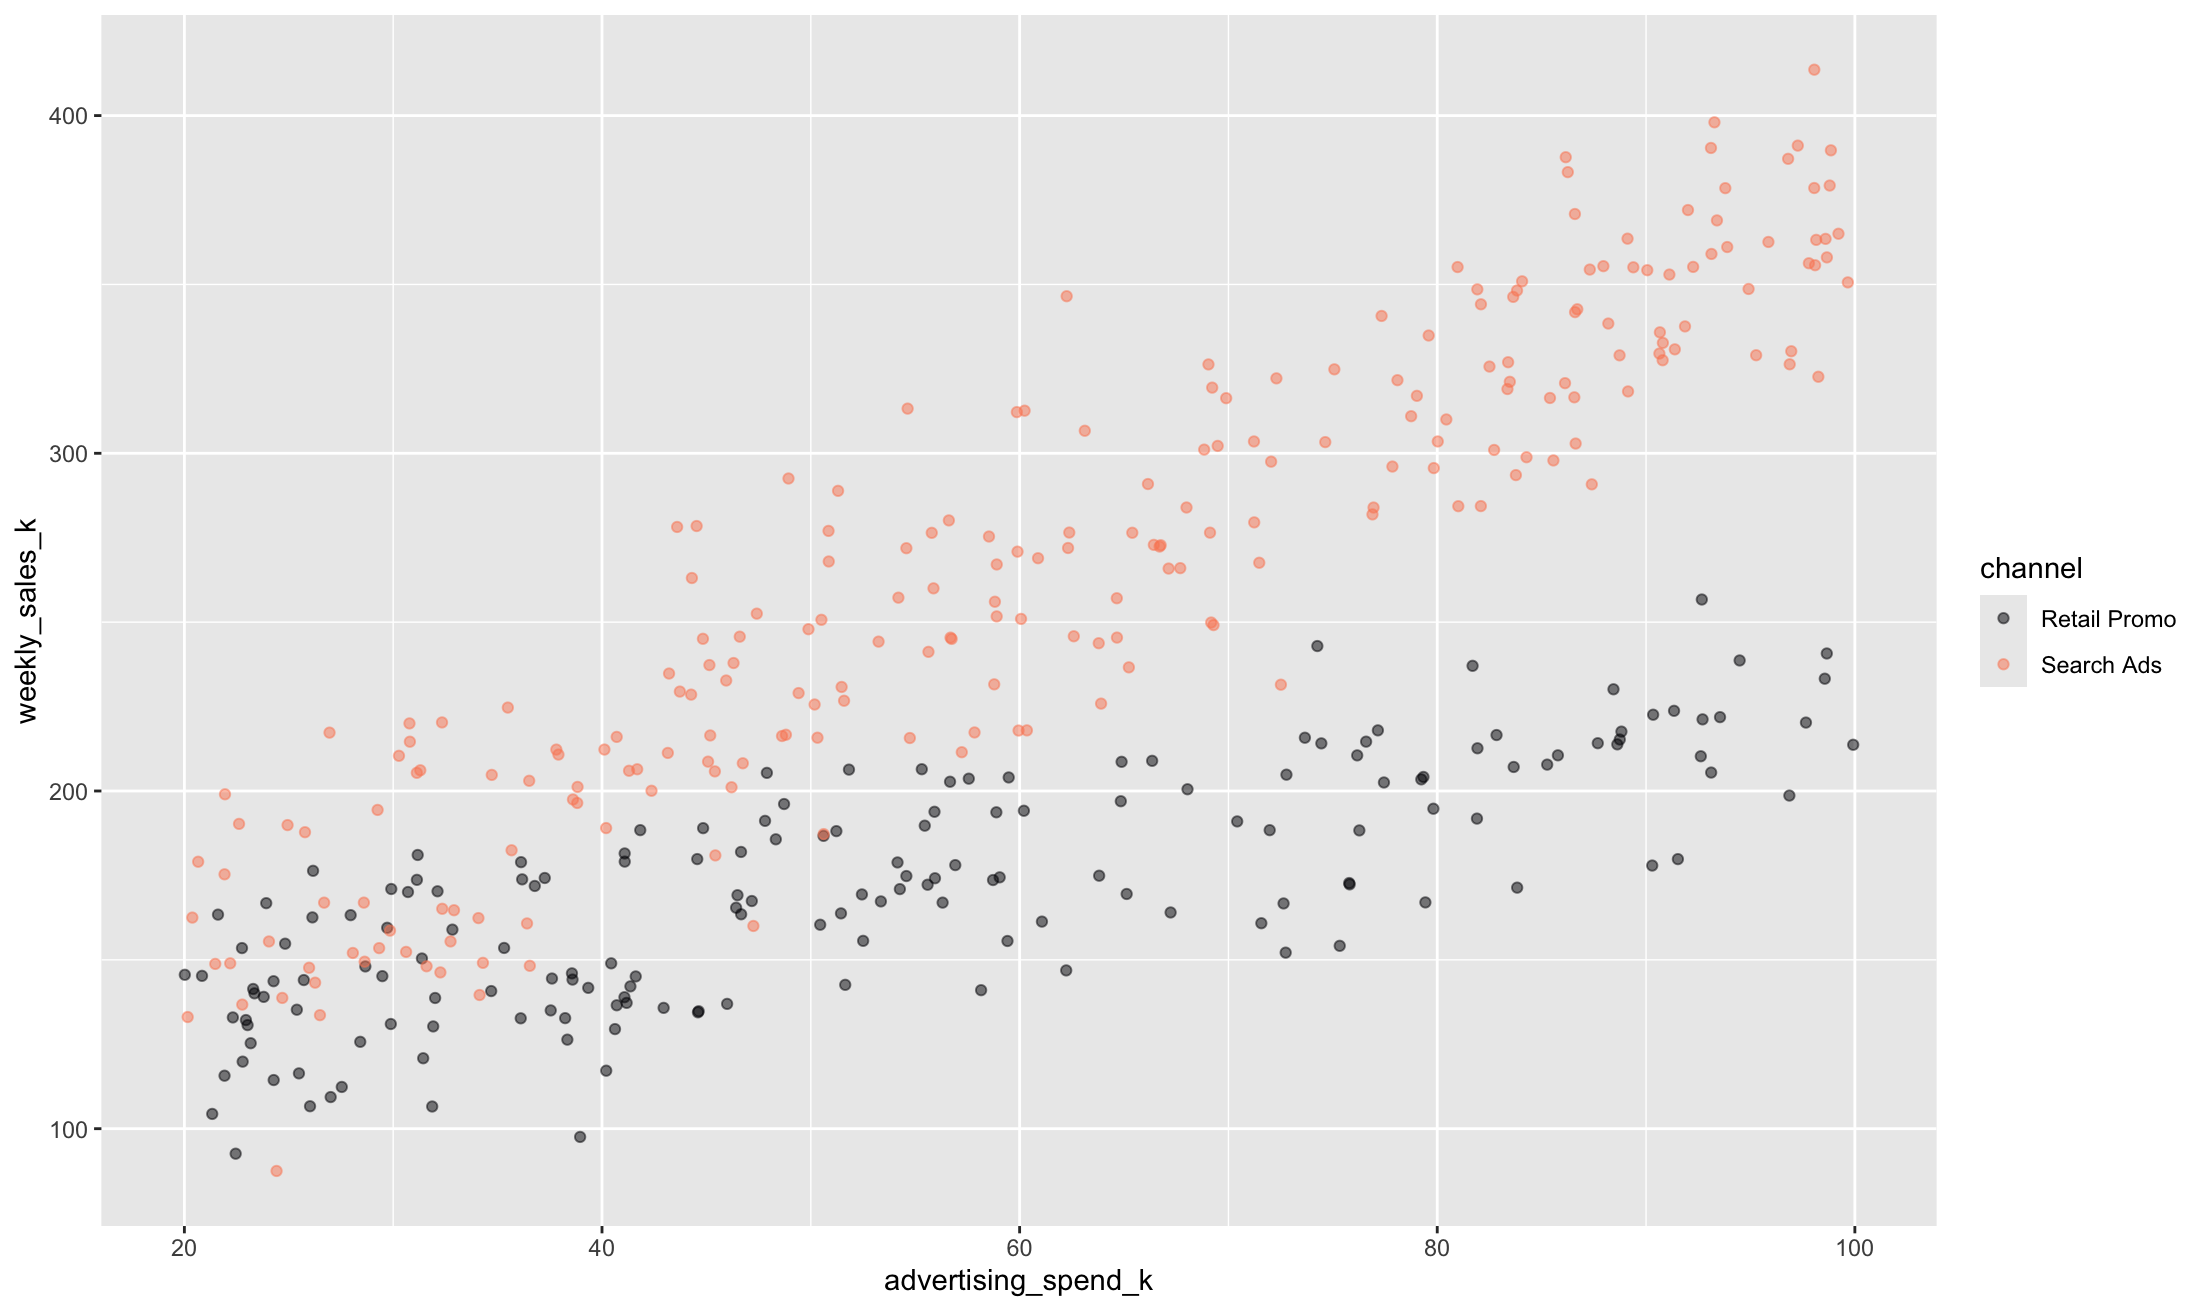
\includegraphics[width=0.7\linewidth,height=\textheight,keepaspectratio]{modules/01-data-visualization/../../images/fig-advertising-sales-channel-color.png}

}

\caption{\label{fig-advertising-sales-channel-color}Determining the
color of points based on a third variable -- the last variable in the
tilde expression for the plot achieves this}

\end{figure}%

Figure~\ref{fig-advertising-sales-channel-color} inserts, through color,
the variable \emph{channel} into the plot of \emph{weekly\_sales\_k}
against \emph{advertising\_spend\_k} from the
\emph{advertising\_sales\_channel} data frame. From it we can clearly
see that the points corresponding to each sales channel clearly shows
the positive relationship that we saw earlier. But this plot also shows
that for a given value of \emph{advertising\_spend\_k} the \emph{Retail
Promo} channel generally has a comparatively higher
\emph{weekly\_sales\_k} value. Adding the variable \emph{channel}
through color enabled us to see more into the data than before.

\subsection{Understanding the tilde expression to add a third
variable}\label{understanding-the-tilde-expression-to-add-a-third-variable}

Figure~\ref{fig-color-tilde-expression} shows the tilde expression we
used in a point plot of two variables to color the points based on a
third variable.

\begin{figure}

\centering{

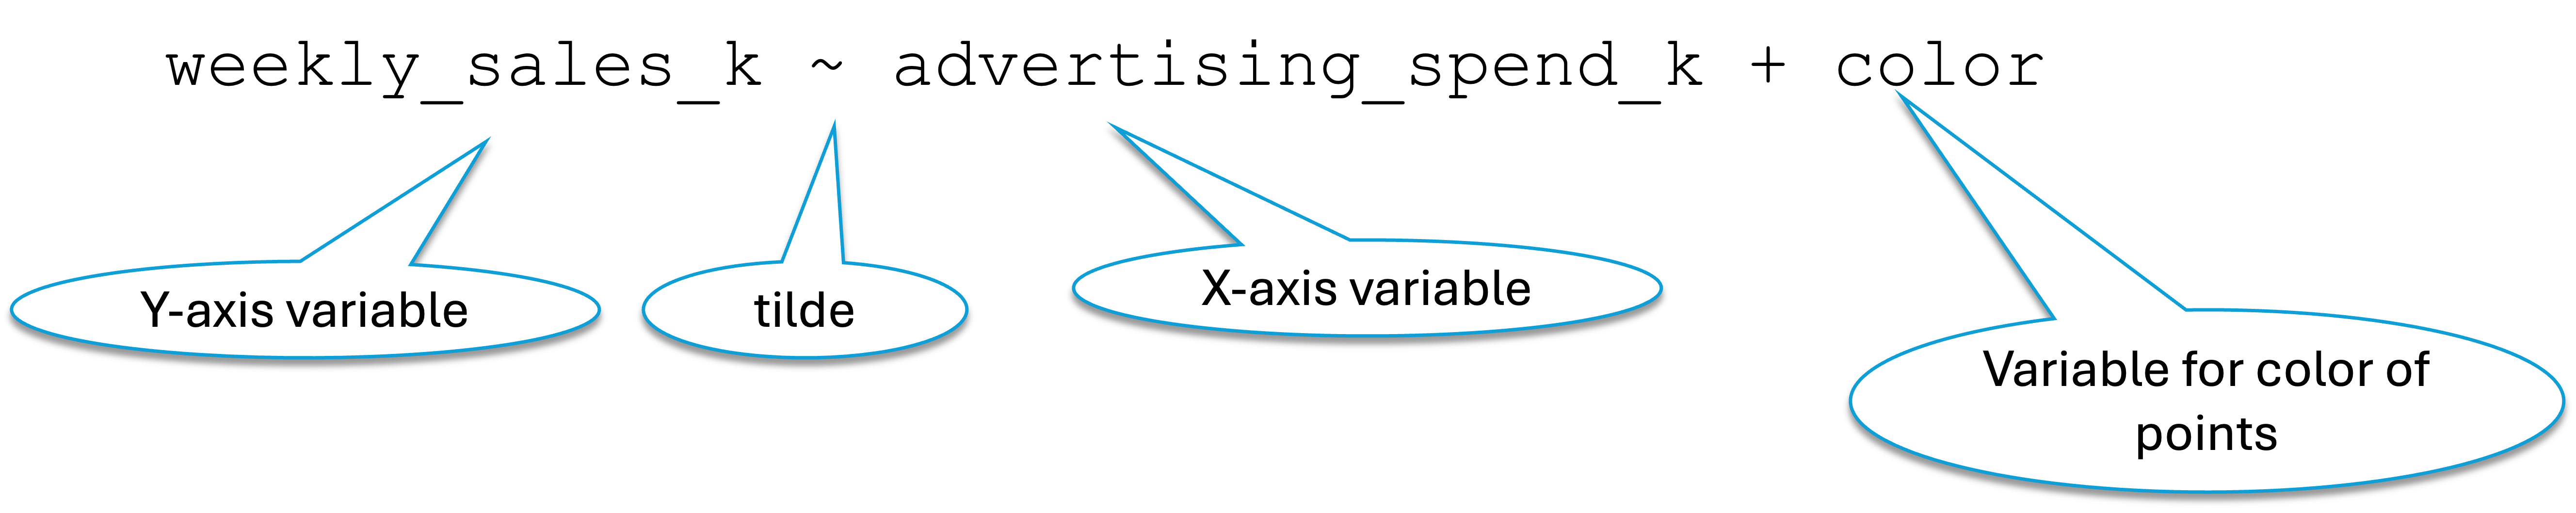
\includegraphics[width=0.7\linewidth,height=\textheight,keepaspectratio]{modules/01-data-visualization/../../images/fig-color-tilde-expression.png}

}

\caption{\label{fig-color-tilde-expression}To color the points based on
the value of a third variable, we just \emph{add} it to the end of the
tilde-expression after a plus sign}

\end{figure}%

Figure~\ref{fig-color-tilde-expression-2} shows another example. In
this, we use the \emph{mpg} data frame which contains data on cars. We
plot the city mileage of cars (variable \emph{cty}) against their engine
displacement (variable \emph{displ}). We color each point based on the
class of the vehicle (variable \emph{class}).

\begin{lstlisting}[language=R]
mpg |> 
  point_plot(cty ~ displ + class)
\end{lstlisting}

\begin{figure}

\centering{

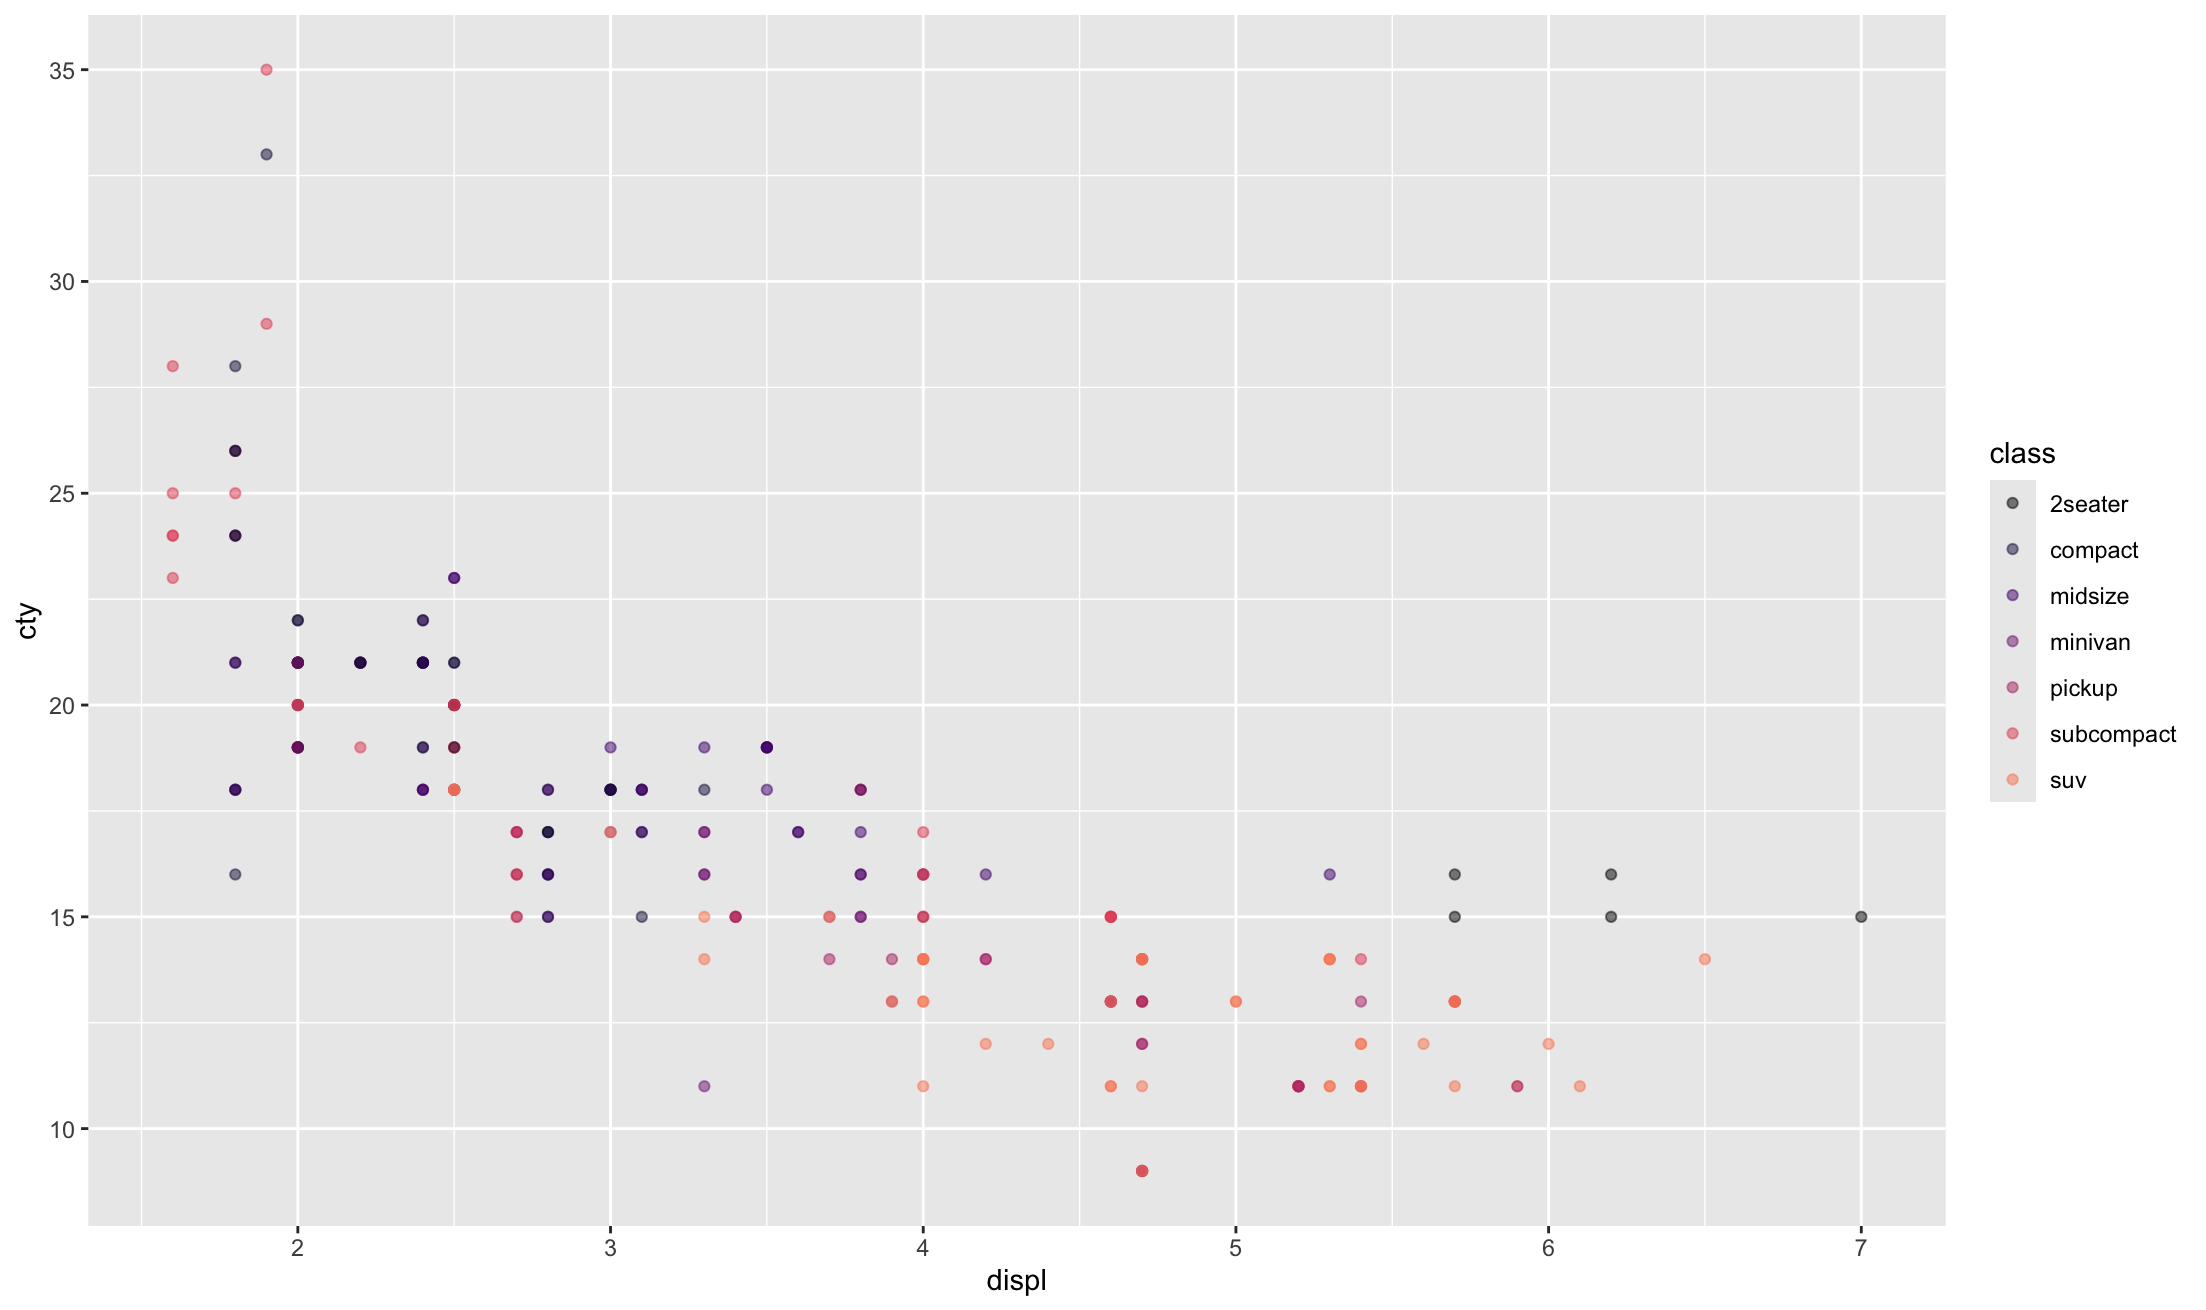
\includegraphics[width=0.7\linewidth,height=\textheight,keepaspectratio]{modules/01-data-visualization/../../images/fig-color-tilde-expression-2.png}

}

\caption{\label{fig-color-tilde-expression-2}The scatterplot shows the
relationship between \emph{displ} and \emph{cty} from the \emph{mpg}
data frame -- the variable \emph{class} in the tilde expression
determines the color of the points}

\end{figure}%

\begin{tcolorbox}[enhanced jigsaw, colback=white, leftrule=.75mm, toprule=.15mm, bottomtitle=1mm, breakable, coltitle=black, toptitle=1mm, title={Quick Check}, opacitybacktitle=0.6, colbacktitle=quarto-callout-note-color!10!white, arc=.35mm, left=2mm, colframe=quarto-callout-note-color-frame, titlerule=0mm, rightrule=.15mm, bottomrule=.15mm, opacityback=0]

In weekly\_sales\_k \textasciitilde{} advertising\_spend\_k + channel,
what does channel control?

\end{tcolorbox}

\begin{tcolorbox}[enhanced jigsaw, colback=white, leftrule=.75mm, toprule=.15mm, bottomtitle=1mm, breakable, coltitle=black, toptitle=1mm, title={Suggested answer}, opacitybacktitle=0.6, colbacktitle=quarto-callout-note-color!10!white, arc=.35mm, left=2mm, colframe=quarto-callout-note-color-frame, titlerule=0mm, rightrule=.15mm, bottomrule=.15mm, opacityback=0]

The color of points.

\end{tcolorbox}

\begin{tcolorbox}[enhanced jigsaw, colback=white, leftrule=.75mm, toprule=.15mm, bottomtitle=1mm, breakable, coltitle=black, toptitle=1mm, title={Quick Check}, opacitybacktitle=0.6, colbacktitle=quarto-callout-note-color!10!white, arc=.35mm, left=2mm, colframe=quarto-callout-note-color-frame, titlerule=0mm, rightrule=.15mm, bottomrule=.15mm, opacityback=0]

What new insight can color reveal that the two-variable plot cannot?

\end{tcolorbox}

\begin{tcolorbox}[enhanced jigsaw, colback=white, leftrule=.75mm, toprule=.15mm, bottomtitle=1mm, breakable, coltitle=black, toptitle=1mm, title={Suggested answer}, opacitybacktitle=0.6, colbacktitle=quarto-callout-note-color!10!white, arc=.35mm, left=2mm, colframe=quarto-callout-note-color-frame, titlerule=0mm, rightrule=.15mm, bottomrule=.15mm, opacityback=0]

Differences in level or pattern between groups (e.g., Retail Promo tends
to have higher sales at the same ad spend).

\end{tcolorbox}

\section{Bringing a fourth variable into
play}\label{bringing-a-fourth-variable-into-play}

We can bring a fourth variable into play as well through \emph{facets}.
Replacing the tilde expression above with:

\begin{lstlisting}
hwy ~ displ + class + drv
\end{lstlisting}

generates Figure~\ref{fig-facet-example-1}.

\begin{figure}

\centering{

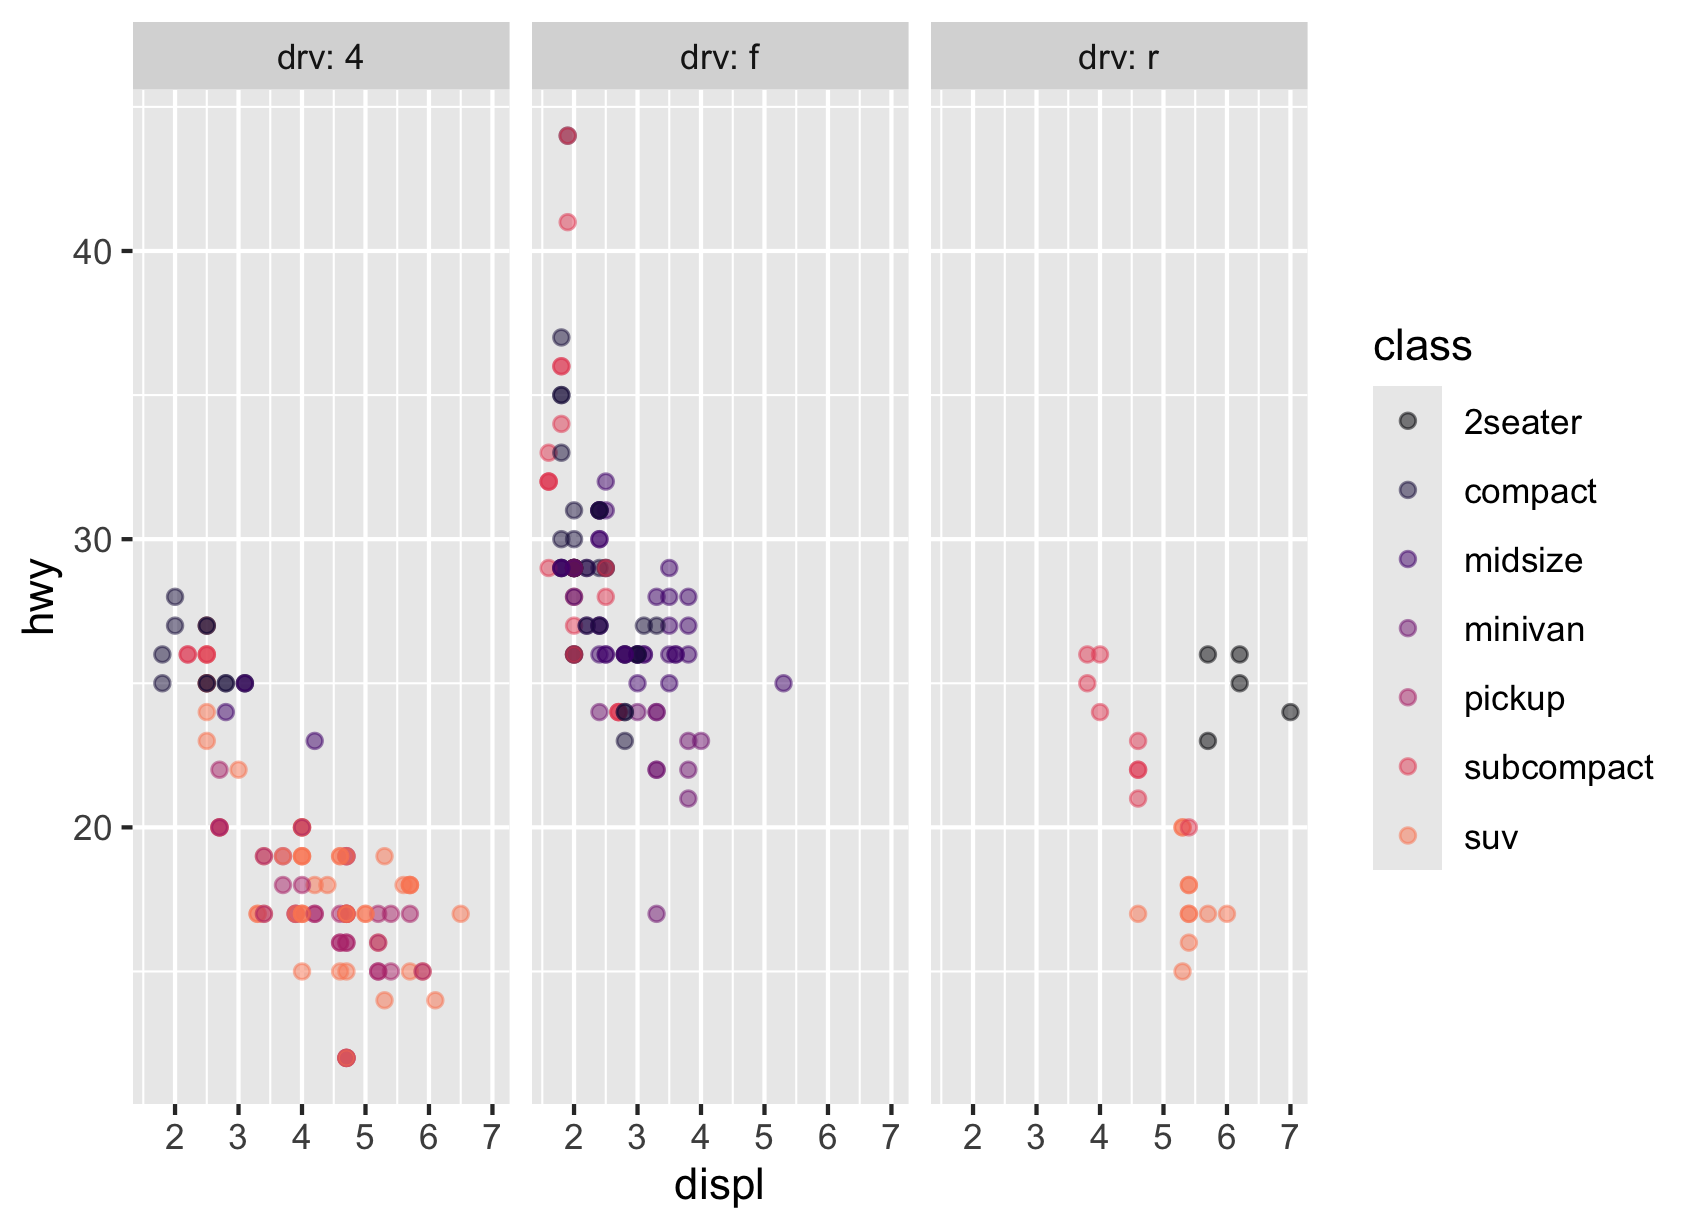
\includegraphics[width=0.7\linewidth,height=\textheight,keepaspectratio]{modules/01-data-visualization/../../images/fig-facet-example-1.png}

}

\caption{\label{fig-facet-example-1}The scatterplot shows the
relationship between \emph{displ} and \emph{cty} from the \emph{mpg}
data frame -- the variable \emph{class} in the tilde expression
determines the color of the points and the variable \emph{drv} divides
the plot into \emph{facets}}

\end{figure}%

In this figure, we use the \emph{mpg} data frame and generate a basic
scatterplot of the relationship between the highway mileage (variable
\emph{hwy}) and the engine displacement (variable\emph{displ}). The
third variable \emph{class} determines the color of the points. The
fourth variable \emph{drv} segments the plots into \emph{facets} -- one
for each possible value of \emph{drv}.

\begin{tcolorbox}[enhanced jigsaw, colback=white, leftrule=.75mm, toprule=.15mm, bottomtitle=1mm, breakable, coltitle=black, toptitle=1mm, title=\textcolor{quarto-callout-important-color}{\faExclamation}\hspace{0.5em}{Important}, opacitybacktitle=0.6, colbacktitle=quarto-callout-important-color!10!white, arc=.35mm, left=2mm, colframe=quarto-callout-important-color-frame, titlerule=0mm, rightrule=.15mm, bottomrule=.15mm, opacityback=0]

\textbf{Tilde expression summary}

y \textasciitilde{} x → y on vertical axis, x on horizontal axis

y \textasciitilde{} x + color → color encodes the third variable

y \textasciitilde{} x + color + facet → facet splits into panels by the
fourth variable

\end{tcolorbox}

\section{Optional enrichment topic: Can a numerical variable be related
to a categorical
one?}\label{optional-enrichment-topic-can-a-numerical-variable-be-related-to-a-categorical-one}

Yes. A numerical variable can be related to a categorical one. For
example, in Figure~\ref{fig-bank-account-type-balance} we see that the
variable \emph{balance} (numerical) differs between the two categories
of the variable \emph{bank\_account\_type} (categorical). The
\emph{Savings} accounts generally have higher balances than
\emph{Checking} accounts.

Figure~\ref{fig-mpg-cty-drv-scatter} shows the relationship between the
city mileage (variable \emph{cty}) and the drive (variable \emph{drv}).

\begin{lstlisting}[language=R]
mpg |> 
  point_plot(cty ~ drv)
\end{lstlisting}

We see a pattern. Front wheel drive cars have a significantly higher
fuel efficiency than the other two types of drive (rear and four wheel
drive).

\begin{figure}

\centering{

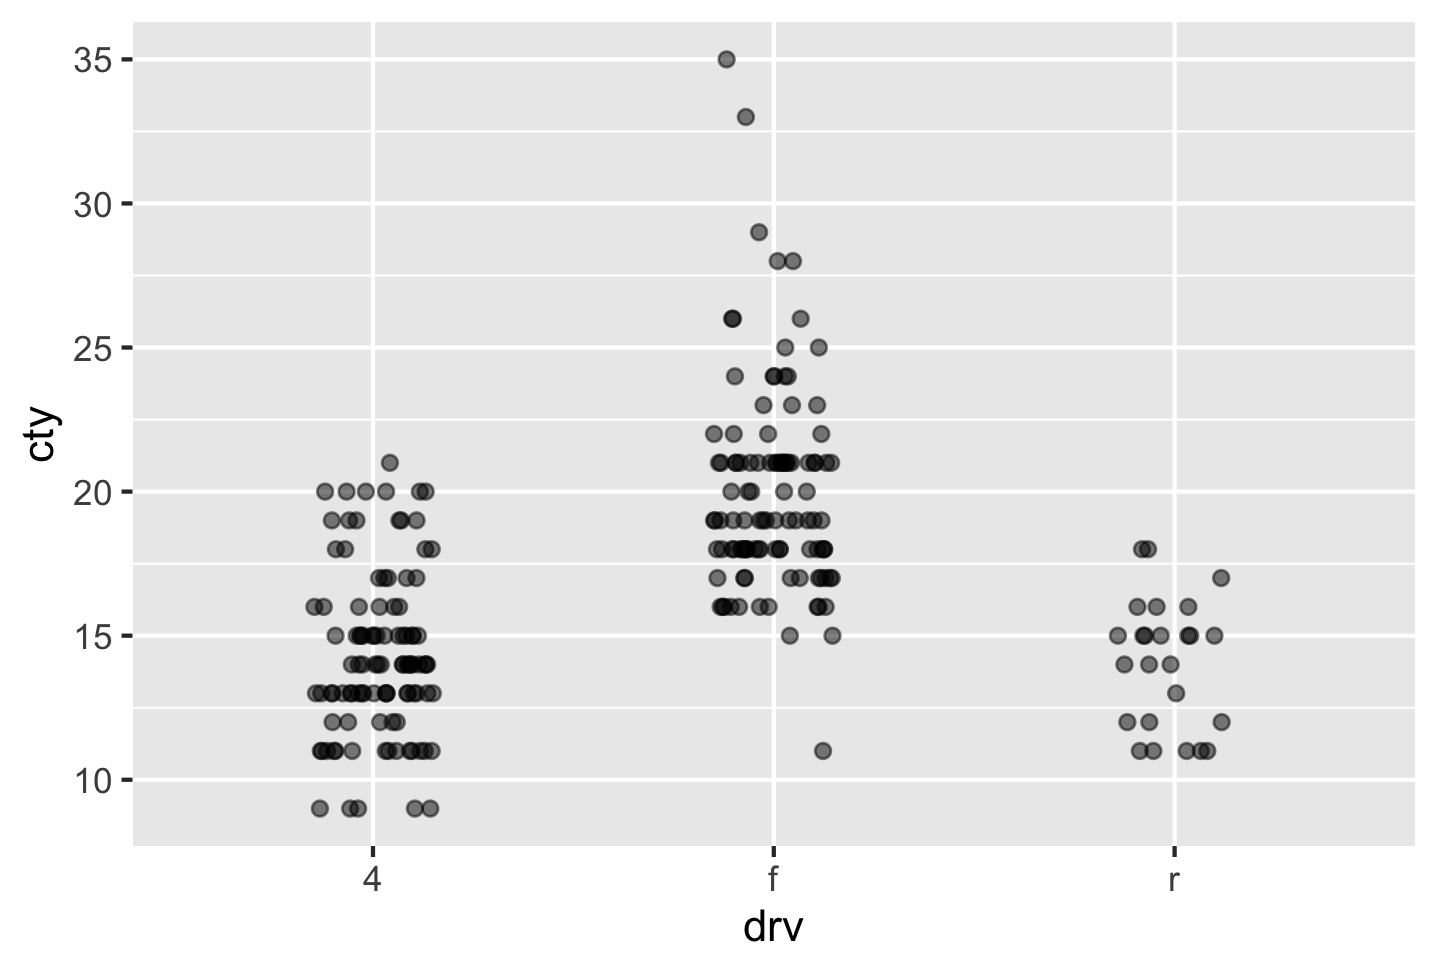
\includegraphics[width=0.7\linewidth,height=\textheight,keepaspectratio]{modules/01-data-visualization/../../images/fig-mpg-cty-drv-scatter.png}

}

\caption{\label{fig-mpg-cty-drv-scatter}Relationship between a numerical
variable \emph{cty} and a caytegorical variable \emph{drv}: from the
\emph{mpg} data frame}

\end{figure}%

Although there is a relationship, we do not use the correlation
coefficient to quantify it. Correlation coefficients are only used for
relationships between two numerical variables. Also recallthat it
measure the strength of a \emph{linear} relationship. Here, with one
variable being categorical, the idea of linearity does not apply.

There is another coefficient called \textbf{eta squared} (η²) that can
be used to quantify the relationship between a numerical and a
categorical variable. We will talk about it in a later chapter under
optional enrichment topics.

\section*{Mini-Review: Scatterplots and
Relationships}\label{mini-review-scatterplots-and-relationships}
\addcontentsline{toc}{section}{Mini-Review: Scatterplots and
Relationships}

\markright{Mini-Review: Scatterplots and Relationships}

\begin{tcolorbox}[enhanced jigsaw, colback=white, leftrule=.75mm, toprule=.15mm, bottomtitle=1mm, breakable, coltitle=black, toptitle=1mm, title=\textcolor{quarto-callout-note-color}{\faInfo}\hspace{0.5em}{Note}, opacitybacktitle=0.6, colbacktitle=quarto-callout-note-color!10!white, arc=.35mm, left=2mm, colframe=quarto-callout-note-color-frame, titlerule=0mm, rightrule=.15mm, bottomrule=.15mm, opacityback=0]

Answer the questions below to check your understanding of how
scatterplots represent data and relationships between variables.

\end{tcolorbox}

\subsection*{Question 1}\label{question-1}
\addcontentsline{toc}{subsection}{Question 1}

In a scatterplot of \passthrough{\lstinline!sales\_qty \~ price!}, what
does the x-coordinate of a point represent?

\begin{tcolorbox}[enhanced jigsaw, colback=white, leftrule=.75mm, toprule=.15mm, bottomtitle=1mm, breakable, coltitle=black, toptitle=1mm, title={Suggested answer}, opacitybacktitle=0.6, colbacktitle=quarto-callout-note-color!10!white, arc=.35mm, left=2mm, colframe=quarto-callout-note-color-frame, titlerule=0mm, rightrule=.15mm, bottomrule=.15mm, opacityback=0]

The x-coordinate represents the value of \passthrough{\lstinline!price!}
for that observation.

\end{tcolorbox}

\begin{center}\rule{0.5\linewidth}{0.5pt}\end{center}

\subsection*{Question 2}\label{question-2}
\addcontentsline{toc}{subsection}{Question 2}

In the same scatterplot, what does the y-coordinate of a point
represent?

\begin{tcolorbox}[enhanced jigsaw, colback=white, leftrule=.75mm, toprule=.15mm, bottomtitle=1mm, breakable, coltitle=black, toptitle=1mm, title={Suggested answer}, opacitybacktitle=0.6, colbacktitle=quarto-callout-note-color!10!white, arc=.35mm, left=2mm, colframe=quarto-callout-note-color-frame, titlerule=0mm, rightrule=.15mm, bottomrule=.15mm, opacityback=0]

The y-coordinate represents the value of
\passthrough{\lstinline!sales\_qty!} for that observation.

\end{tcolorbox}

\begin{center}\rule{0.5\linewidth}{0.5pt}\end{center}

\subsection*{Question 3}\label{question-3}
\addcontentsline{toc}{subsection}{Question 3}

If a scatterplot is based on a data frame with 500 rows, how many points
appear in the plot?

\begin{tcolorbox}[enhanced jigsaw, colback=white, leftrule=.75mm, toprule=.15mm, bottomtitle=1mm, breakable, coltitle=black, toptitle=1mm, title={Suggested answer}, opacitybacktitle=0.6, colbacktitle=quarto-callout-note-color!10!white, arc=.35mm, left=2mm, colframe=quarto-callout-note-color-frame, titlerule=0mm, rightrule=.15mm, bottomrule=.15mm, opacityback=0]

500 points --- one for each row of the data frame.

\end{tcolorbox}

\begin{center}\rule{0.5\linewidth}{0.5pt}\end{center}

\subsection*{Question 4}\label{question-4}
\addcontentsline{toc}{subsection}{Question 4}

Describe how you would locate on the plot the point corresponding to a
row with\\
\passthrough{\lstinline!price = 12.5!} and
\passthrough{\lstinline!sales\_qty = 1200!}.

\begin{tcolorbox}[enhanced jigsaw, colback=white, leftrule=.75mm, toprule=.15mm, bottomtitle=1mm, breakable, coltitle=black, toptitle=1mm, title={Suggested answer}, opacitybacktitle=0.6, colbacktitle=quarto-callout-note-color!10!white, arc=.35mm, left=2mm, colframe=quarto-callout-note-color-frame, titlerule=0mm, rightrule=.15mm, bottomrule=.15mm, opacityback=0]

Locate 12.5 on the x-axis, move vertically until reaching 1200 on the
y-axis, and mark the intersection.

\end{tcolorbox}

\begin{center}\rule{0.5\linewidth}{0.5pt}\end{center}

\subsection*{Question 5}\label{question-5}
\addcontentsline{toc}{subsection}{Question 5}

What visual pattern indicates a \textbf{negative relationship} between
two numerical variables?

\begin{tcolorbox}[enhanced jigsaw, colback=white, leftrule=.75mm, toprule=.15mm, bottomtitle=1mm, breakable, coltitle=black, toptitle=1mm, title={Suggested answer}, opacitybacktitle=0.6, colbacktitle=quarto-callout-note-color!10!white, arc=.35mm, left=2mm, colframe=quarto-callout-note-color-frame, titlerule=0mm, rightrule=.15mm, bottomrule=.15mm, opacityback=0]

A downward-sloping cloud of points: as x increases, y generally
decreases.

\end{tcolorbox}

\begin{center}\rule{0.5\linewidth}{0.5pt}\end{center}

\subsection*{Question 6}\label{question-6}
\addcontentsline{toc}{subsection}{Question 6}

What does it mean if a scatterplot shows \textbf{no clear trend}?

\begin{tcolorbox}[enhanced jigsaw, colback=white, leftrule=.75mm, toprule=.15mm, bottomtitle=1mm, breakable, coltitle=black, toptitle=1mm, title={Suggested answer}, opacitybacktitle=0.6, colbacktitle=quarto-callout-note-color!10!white, arc=.35mm, left=2mm, colframe=quarto-callout-note-color-frame, titlerule=0mm, rightrule=.15mm, bottomrule=.15mm, opacityback=0]

There is no apparent linear relationship --- higher or lower values of
one variable do not predict higher or lower values of the other.

\end{tcolorbox}

\begin{center}\rule{0.5\linewidth}{0.5pt}\end{center}

\subsection*{Question 7}\label{question-7}
\addcontentsline{toc}{subsection}{Question 7}

What does the \textbf{sign} of the correlation coefficient tell you?

\begin{tcolorbox}[enhanced jigsaw, colback=white, leftrule=.75mm, toprule=.15mm, bottomtitle=1mm, breakable, coltitle=black, toptitle=1mm, title={Suggested answer}, opacitybacktitle=0.6, colbacktitle=quarto-callout-note-color!10!white, arc=.35mm, left=2mm, colframe=quarto-callout-note-color-frame, titlerule=0mm, rightrule=.15mm, bottomrule=.15mm, opacityback=0]

It tells you the direction of the linear relationship: positive for
upward trends and negative for downward trends.

\end{tcolorbox}

\begin{center}\rule{0.5\linewidth}{0.5pt}\end{center}

\subsection*{Question 8}\label{question-8}
\addcontentsline{toc}{subsection}{Question 8}

A correlation coefficient close to 0 means what?

\begin{tcolorbox}[enhanced jigsaw, colback=white, leftrule=.75mm, toprule=.15mm, bottomtitle=1mm, breakable, coltitle=black, toptitle=1mm, title={Suggested answer}, opacitybacktitle=0.6, colbacktitle=quarto-callout-note-color!10!white, arc=.35mm, left=2mm, colframe=quarto-callout-note-color-frame, titlerule=0mm, rightrule=.15mm, bottomrule=.15mm, opacityback=0]

There is little or no \textbf{linear} relationship between the
variables, even though a nonlinear relationship may still exist.

\end{tcolorbox}

\begin{center}\rule{0.5\linewidth}{0.5pt}\end{center}

\subsection*{Question 9}\label{question-9}
\addcontentsline{toc}{subsection}{Question 9}

Why does \passthrough{\lstinline!point\_plot()!} jitter points when the
x-axis variable is categorical?

\begin{tcolorbox}[enhanced jigsaw, colback=white, leftrule=.75mm, toprule=.15mm, bottomtitle=1mm, breakable, coltitle=black, toptitle=1mm, title={Suggested answer}, opacitybacktitle=0.6, colbacktitle=quarto-callout-note-color!10!white, arc=.35mm, left=2mm, colframe=quarto-callout-note-color-frame, titlerule=0mm, rightrule=.15mm, bottomrule=.15mm, opacityback=0]

To reduce over plotting so that points with the same category and
similar values do not overlap visually.

\end{tcolorbox}

\begin{center}\rule{0.5\linewidth}{0.5pt}\end{center}

\subsection*{Question 10}\label{question-10}
\addcontentsline{toc}{subsection}{Question 10}

In the formula\\
\passthrough{\lstinline!weekly\_sales\_k \~ advertising\_spend\_k + channel!},\\
what role does \passthrough{\lstinline!channel!} play in the plot?

\begin{tcolorbox}[enhanced jigsaw, colback=white, leftrule=.75mm, toprule=.15mm, bottomtitle=1mm, breakable, coltitle=black, toptitle=1mm, title={Suggested answer}, opacitybacktitle=0.6, colbacktitle=quarto-callout-note-color!10!white, arc=.35mm, left=2mm, colframe=quarto-callout-note-color-frame, titlerule=0mm, rightrule=.15mm, bottomrule=.15mm, opacityback=0]

It determines the color of the points, allowing different groups to be
distinguished visually.

\end{tcolorbox}

\begin{center}\rule{0.5\linewidth}{0.5pt}\end{center}

\subsection*{Question 11}\label{question-11}
\addcontentsline{toc}{subsection}{Question 11}

What additional role does a fourth variable play when added as\\
\passthrough{\lstinline!y \~ x + color\_var + z!}?

\begin{tcolorbox}[enhanced jigsaw, colback=white, leftrule=.75mm, toprule=.15mm, bottomtitle=1mm, breakable, coltitle=black, toptitle=1mm, title={Suggested answer}, opacitybacktitle=0.6, colbacktitle=quarto-callout-note-color!10!white, arc=.35mm, left=2mm, colframe=quarto-callout-note-color-frame, titlerule=0mm, rightrule=.15mm, bottomrule=.15mm, opacityback=0]

It divides the plot into separate panels (facets), one for each value of
the fourth variable.

\end{tcolorbox}

\part{Variation}

\chapter*{Module 2: Variation}\label{module-2-variation}
\addcontentsline{toc}{chapter}{Module 2: Variation}

\markboth{Module 2: Variation}{Module 2: Variation}

Variation plays a very important role in statistics. Some even go to the
extent of viewing the discipline of statistics itself as the study of
variation.

This module discusses variation generally by visualizing it through
\emph{violin} plots. It then introduces the key statistical concepts of
\emph{variance} and \emph{standard deviation} and how to compute these
using R.

\section*{Learning Goals}\label{learning-goals-1}
\addcontentsline{toc}{section}{Learning Goals}

\markright{Learning Goals}

\begin{itemize}
\tightlist
\item
  Explain what variability in a variable represents
\item
  Plot and interpret violin plots
\item
  Identify broad characteristics of distribution shapes
\item
  Compute variance and standard deviation of a small set of numbers by
  hand
\item
  Use R to compute the variance and standard deviation of variables in a
  data frame
\item
\end{itemize}

\section*{Structure of This Module}\label{structure-of-this-module-1}
\addcontentsline{toc}{section}{Structure of This Module}

\markright{Structure of This Module}

\begin{itemize}
\tightlist
\item
  Violin plots
\item
  Variance and standard deviation
\end{itemize}

\chapter{Using Violin Plots to Visualize
Distribution}\label{using-violin-plots-to-visualize-distribution}

This chapter talks about visualizing variability.

\section*{Learning outcomes}\label{learning-outcomes-2}
\addcontentsline{toc}{section}{Learning outcomes}

\markright{Learning outcomes}

\subsection*{After completing this chapter you will be able
to:}\label{after-completing-this-chapter-you-will-be-able-to}
\addcontentsline{toc}{subsection}{After completing this chapter you will
be able to:}

\textbf{Demonstrate these outcomes related to shapes of distributions:}

\begin{itemize}
\tightlist
\item
  Given a distribution as histogram, explain what the height of a bar
  represents
\item
  Given a distribution as a violin plot, explain what the width of a
  violin at any point represents
\item
  Given a violin plot, identify the point(s) having the highest and
  lowest densities
\item
  Identify whether a given distribution shown either as a histogram or
  as a violin plot or as a density plot is

  \begin{itemize}
  \tightlist
  \item
    uniform
  \item
    symmetric bell shaped
  \item
    multi-modal
  \item
    skewed and in which way
  \end{itemize}
\end{itemize}

\textbf{Demonstrate these outcomes related to generating violin plots
using R:}

\begin{itemize}
\tightlist
\item
  Given a data frame and a numerical variable, write R code to generate
  a violin plot to study the distribution of the variable
\item
  Explain the two important parts of the plot area in a violin plot
\item
  In the plot, identify which part represents the data and which part
  represents the \emph{annotation}
\item
  Explain the tilde expression used to generate violin plots of single
  variables
\item
  Generate a violin plot to compare the distributions of a single
  numerical variable corresponding to a categorical variable
\end{itemize}

We have already looks at the concept of \emph{variable}. We have used
the term to refer to a column of a data frame. We explained the
rationale for the name from the fact that the values in a single column
of a data frame \emph{vary}. That is, not all the rows of a column have
the same value. For example, we see in Table~\ref{tbl-boston-marathon-2}
that the values in the column \emph{minutes} vary -- that is, not all
the values in the column are the same. The same is true of every column.

\begin{longtable}[]{@{}
  >{\raggedleft\arraybackslash}p{(\linewidth - 10\tabcolsep) * \real{0.0725}}
  >{\raggedright\arraybackslash}p{(\linewidth - 10\tabcolsep) * \real{0.3768}}
  >{\raggedright\arraybackslash}p{(\linewidth - 10\tabcolsep) * \real{0.2029}}
  >{\raggedright\arraybackslash}p{(\linewidth - 10\tabcolsep) * \real{0.1304}}
  >{\raggedright\arraybackslash}p{(\linewidth - 10\tabcolsep) * \real{0.1014}}
  >{\raggedleft\arraybackslash}p{(\linewidth - 10\tabcolsep) * \real{0.1159}}@{}}

\caption{\label{tbl-boston-marathon-2}Boston Marathon data (20 randonmly
selected rows).}

\tabularnewline

\toprule\noalign{}
\begin{minipage}[b]{\linewidth}\raggedleft
year
\end{minipage} & \begin{minipage}[b]{\linewidth}\raggedright
name
\end{minipage} & \begin{minipage}[b]{\linewidth}\raggedright
country
\end{minipage} & \begin{minipage}[b]{\linewidth}\raggedright
time
\end{minipage} & \begin{minipage}[b]{\linewidth}\raggedright
sex
\end{minipage} & \begin{minipage}[b]{\linewidth}\raggedleft
minutes
\end{minipage} \\
\midrule\noalign{}
\endhead
\bottomrule\noalign{}
\endlastfoot
2000 & Elijah Lagat & Kenya & 02:09:47 & male & 130 \\
2009 & Deriba Merga & Ethiopia & 02:08:42 & male & 129 \\
2015 & Lelisa Desisa & Ethiopia & 02:09:17 & male & 129 \\
1970 & Ron Hill & England & 02:10:30 & male & 130 \\
1969 & Yoshiaki Unetani & Japan & 02:13:49 & male & 134 \\
1966 & Kenji Kimihara & Japan & 02:17:11 & male & 137 \\
1977 & Michiko (Miki) Gorman & United States & 02:48:33 & female &
169 \\
1995 & Uta Pippig & Germany & 02:25:11 & female & 145 \\
1982 & Charlotte Teske & Germany & 02:29:33 & female & 150 \\
2015 & Caroline Rotich & Kenya & 02:24:55 & female & 145 \\
2006 & Robert Kipkoech Cheruiyot & Kenya & 02:07:14 & male & 127 \\
1997 & Fatuma Roba & Ethiopia & 02:26:23 & female & 146 \\
1995 & Cosmas Ndeti & Kenya & 02:09:22 & male & 129 \\
2010 & Teyba Erkesso & Ethiopia & 02:26:11 & female & 146 \\
2000 & Catherine Ndereba & Kenya & 02:26:11 & female & 146 \\
1991 & Wanda Panfil & Poland & 02:24:18 & female & 144 \\
1957 & John J. Kelley & United States & 02:20:05 & male & 140 \\
1922 & Clarence H. DeMar & United States & 02:18:10 & male & 138 \\
1964 & Aurele Vandendriessche & Belgium & 02:19:59 & male & 140 \\
1903 & John C. Lorden & United States & 02:41:29 & male & 161 \\

\end{longtable}

Take care to note that we are not saying that every value in a column
has to be distinct. Values can repeat. However we have variety in a
column as long as all the values are not the same. Very rarely will you
come across data frames in which all the values of a column are the
same. In this case the column does not serve any useful purpose for data
analysis.

In this course, we deal only with variability in numerical variables.
Statistics deals with variability in categorical variables as well, but
this book does not consider this in any depth.

\section{Distribution}\label{distribution}

Consider a variable with maximum value of 200 and minimum value 10. Let
us suppose that we have 500 values for this variable (500 rows in the
data frame). This means that the 500 values are all in the range 10 to
200.

We are interested in knowing how these 500 numbers are
\emph{distributed} across the range of 10 to 200.

\begin{itemize}
\tightlist
\item
  It could be the case that the 500 numbers are more or less uniformly
  distributed over their range with approximately the same number of
  occurrences throughout the range.\\
\item
  It could also be the case that the numbers are mostly concentrated in
  the middle -- near 105 or so and as we go further away in either
  direction, the concentration of numbers drops off.
\item
  Or the numbers could be crowded near, the lower extreme, sat at around
  50 or so and be much more sparse away from this point.
\item
  Or it could be that there is heavy concentration around 50 and 150 and
  less elsewhere.
\end{itemize}

The pattern of concentration of values of a variable across its entire
range is called the \textbf{distribution} of the variable.

In this chapter we focus on visualization alone. The next chapter goes
into measuring variation precisely.

\begin{tcolorbox}[enhanced jigsaw, colback=white, leftrule=.75mm, toprule=.15mm, bottomtitle=1mm, breakable, coltitle=black, toptitle=1mm, title={Quick Check}, opacitybacktitle=0.6, colbacktitle=quarto-callout-note-color!10!white, arc=.35mm, left=2mm, colframe=quarto-callout-note-color-frame, titlerule=0mm, rightrule=.15mm, bottomrule=.15mm, opacityback=0]

In your own words, what does it mean to say a variable has a
distribution?

\end{tcolorbox}

\begin{tcolorbox}[enhanced jigsaw, colback=white, leftrule=.75mm, toprule=.15mm, bottomtitle=1mm, breakable, coltitle=black, toptitle=1mm, title={Suggested answer}, opacitybacktitle=0.6, colbacktitle=quarto-callout-note-color!10!white, arc=.35mm, left=2mm, colframe=quarto-callout-note-color-frame, titlerule=0mm, rightrule=.15mm, bottomrule=.15mm, opacityback=0]

A distribution describes how often different values of a variable occur
and how those values are spread out across their range.

\end{tcolorbox}

\begin{tcolorbox}[enhanced jigsaw, colback=white, leftrule=.75mm, toprule=.15mm, bottomtitle=1mm, breakable, coltitle=black, toptitle=1mm, title={Quick Check}, opacitybacktitle=0.6, colbacktitle=quarto-callout-note-color!10!white, arc=.35mm, left=2mm, colframe=quarto-callout-note-color-frame, titlerule=0mm, rightrule=.15mm, bottomrule=.15mm, opacityback=0]

Why is it misleading to describe a data set using only a single number
like the mean?

\end{tcolorbox}

\begin{tcolorbox}[enhanced jigsaw, colback=white, leftrule=.75mm, toprule=.15mm, bottomtitle=1mm, breakable, coltitle=black, toptitle=1mm, title={Suggested answer}, opacitybacktitle=0.6, colbacktitle=quarto-callout-note-color!10!white, arc=.35mm, left=2mm, colframe=quarto-callout-note-color-frame, titlerule=0mm, rightrule=.15mm, bottomrule=.15mm, opacityback=0]

Because very different data sets can share the same mean while having
different spreads, shapes, or extreme values.

\end{tcolorbox}

\begin{tcolorbox}[enhanced jigsaw, colback=white, leftrule=.75mm, toprule=.15mm, bottomtitle=1mm, breakable, coltitle=black, toptitle=1mm, title={Quick Check}, opacitybacktitle=0.6, colbacktitle=quarto-callout-note-color!10!white, arc=.35mm, left=2mm, colframe=quarto-callout-note-color-frame, titlerule=0mm, rightrule=.15mm, bottomrule=.15mm, opacityback=0]

How does a distribution answer the question: ``What values are
typical?''

\end{tcolorbox}

\begin{tcolorbox}[enhanced jigsaw, colback=white, leftrule=.75mm, toprule=.15mm, bottomtitle=1mm, breakable, coltitle=black, toptitle=1mm, title={Suggested answer}, opacitybacktitle=0.6, colbacktitle=quarto-callout-note-color!10!white, arc=.35mm, left=2mm, colframe=quarto-callout-note-color-frame, titlerule=0mm, rightrule=.15mm, bottomrule=.15mm, opacityback=0]

It shows where values cluster most densely and which values occur
rarely.

\end{tcolorbox}

\subsection{Uniform distribution}\label{uniform-distribution}

Suppose we have 1000 numbers with each one being an integer between 1
and 100. Some of the numbers in this data might be 45, 23, 46, 89, 1,
23, 45, 56, and so on. If each number occurs exactly 10 times -- that is
we have 10 ones, 10 twos and so on up to 10 hundreds, we have what is
called as the \emph{uniform distribution}. In a uniform distribution,
each number in the range of the list occurs the same number of times.

Figure~\ref{fig-perfect-uniform-hist} shows a \emph{histogram} of a set
of numbers. A \emph{histogram} breaks up the whole range of the data
points into \emph{bins}. In our example, the numbers range from 1 to
100. A histogram might break this up into some number of \emph{bins}. If
the number of bins is 10, then the numbers between 1 and 10 will fall
unto 1 bin. The numbers between 11 and 20 into the next bin and so on.
In this example, the bin-width is 10 because each bin spans a range of
size 10. The x-axis of the histogram shows the number values and a bar
for each bin. The y axis shows how many of the numbers fall into each
bin and so the pattern formed by the heights of the bars helps us to see
the \emph{distribution} of the numbers.

Figure~\ref{fig-perfect-uniform-hist} shows numbers that are perfectly
uniformly distributed. We have used a bin-width of 1 to have each
individual integer fall into its own bin. In a \emph{uniform
distribution} every number in the overall range of the numbers occurs
exactly the same number of times.

\begin{figure}

\centering{

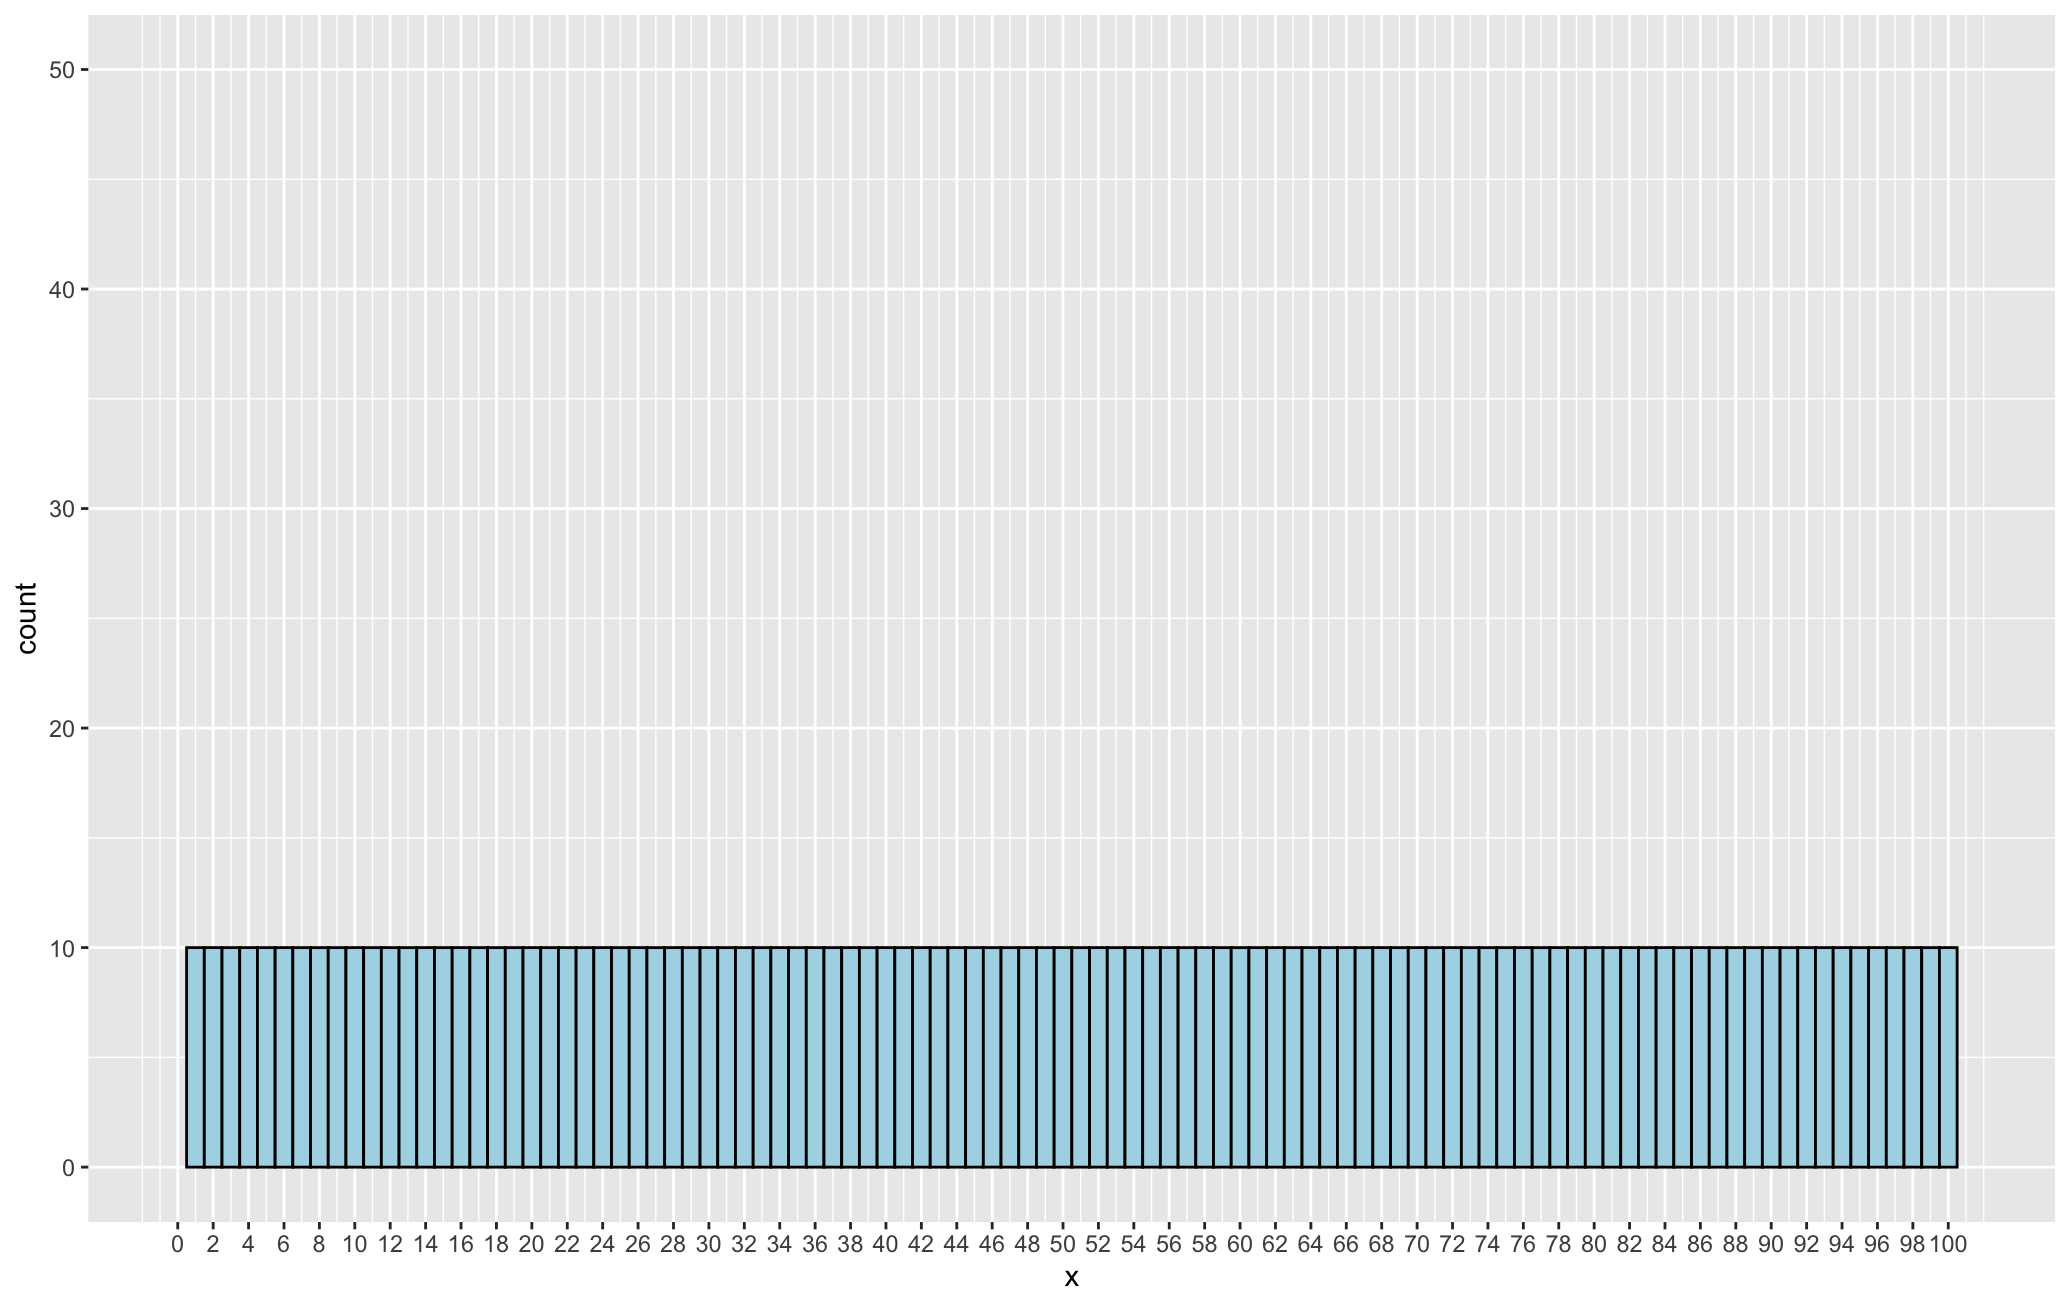
\includegraphics[width=0.7\linewidth,height=\textheight,keepaspectratio]{modules/02-variability/../../images/fig-perfect-uniform-hist.png}

}

\caption{\label{fig-perfect-uniform-hist}Perfect uniform distribution --
each number between 1 and 100 occurs the same number of times (10
times), as you can see from the height of the bars}

\end{figure}%

Our current example deals with integers, but in general when we have
numerical variables, we will deal with numbers that also have a
fractional part. Histograms work in the same way for those too, except
that we cannot have one bin for each distinct value as there is
potentially an infinite number of values in any range.

Figure~\ref{fig-approx-uniform-hist} shows an example of a set of
numbers distributed approximately uniformly. For example, Each number
does not occur exactly the same number of times, but they are loosely
similar. For example, the number 2 seems to appear around 13 times and
the number 25 seems to occur around 18 times. In practice, uniformly
distributed numbers will look more like
Figure~\ref{fig-approx-uniform-hist} than
Figure~\ref{fig-perfect-uniform-hist}.

\begin{figure}

\centering{

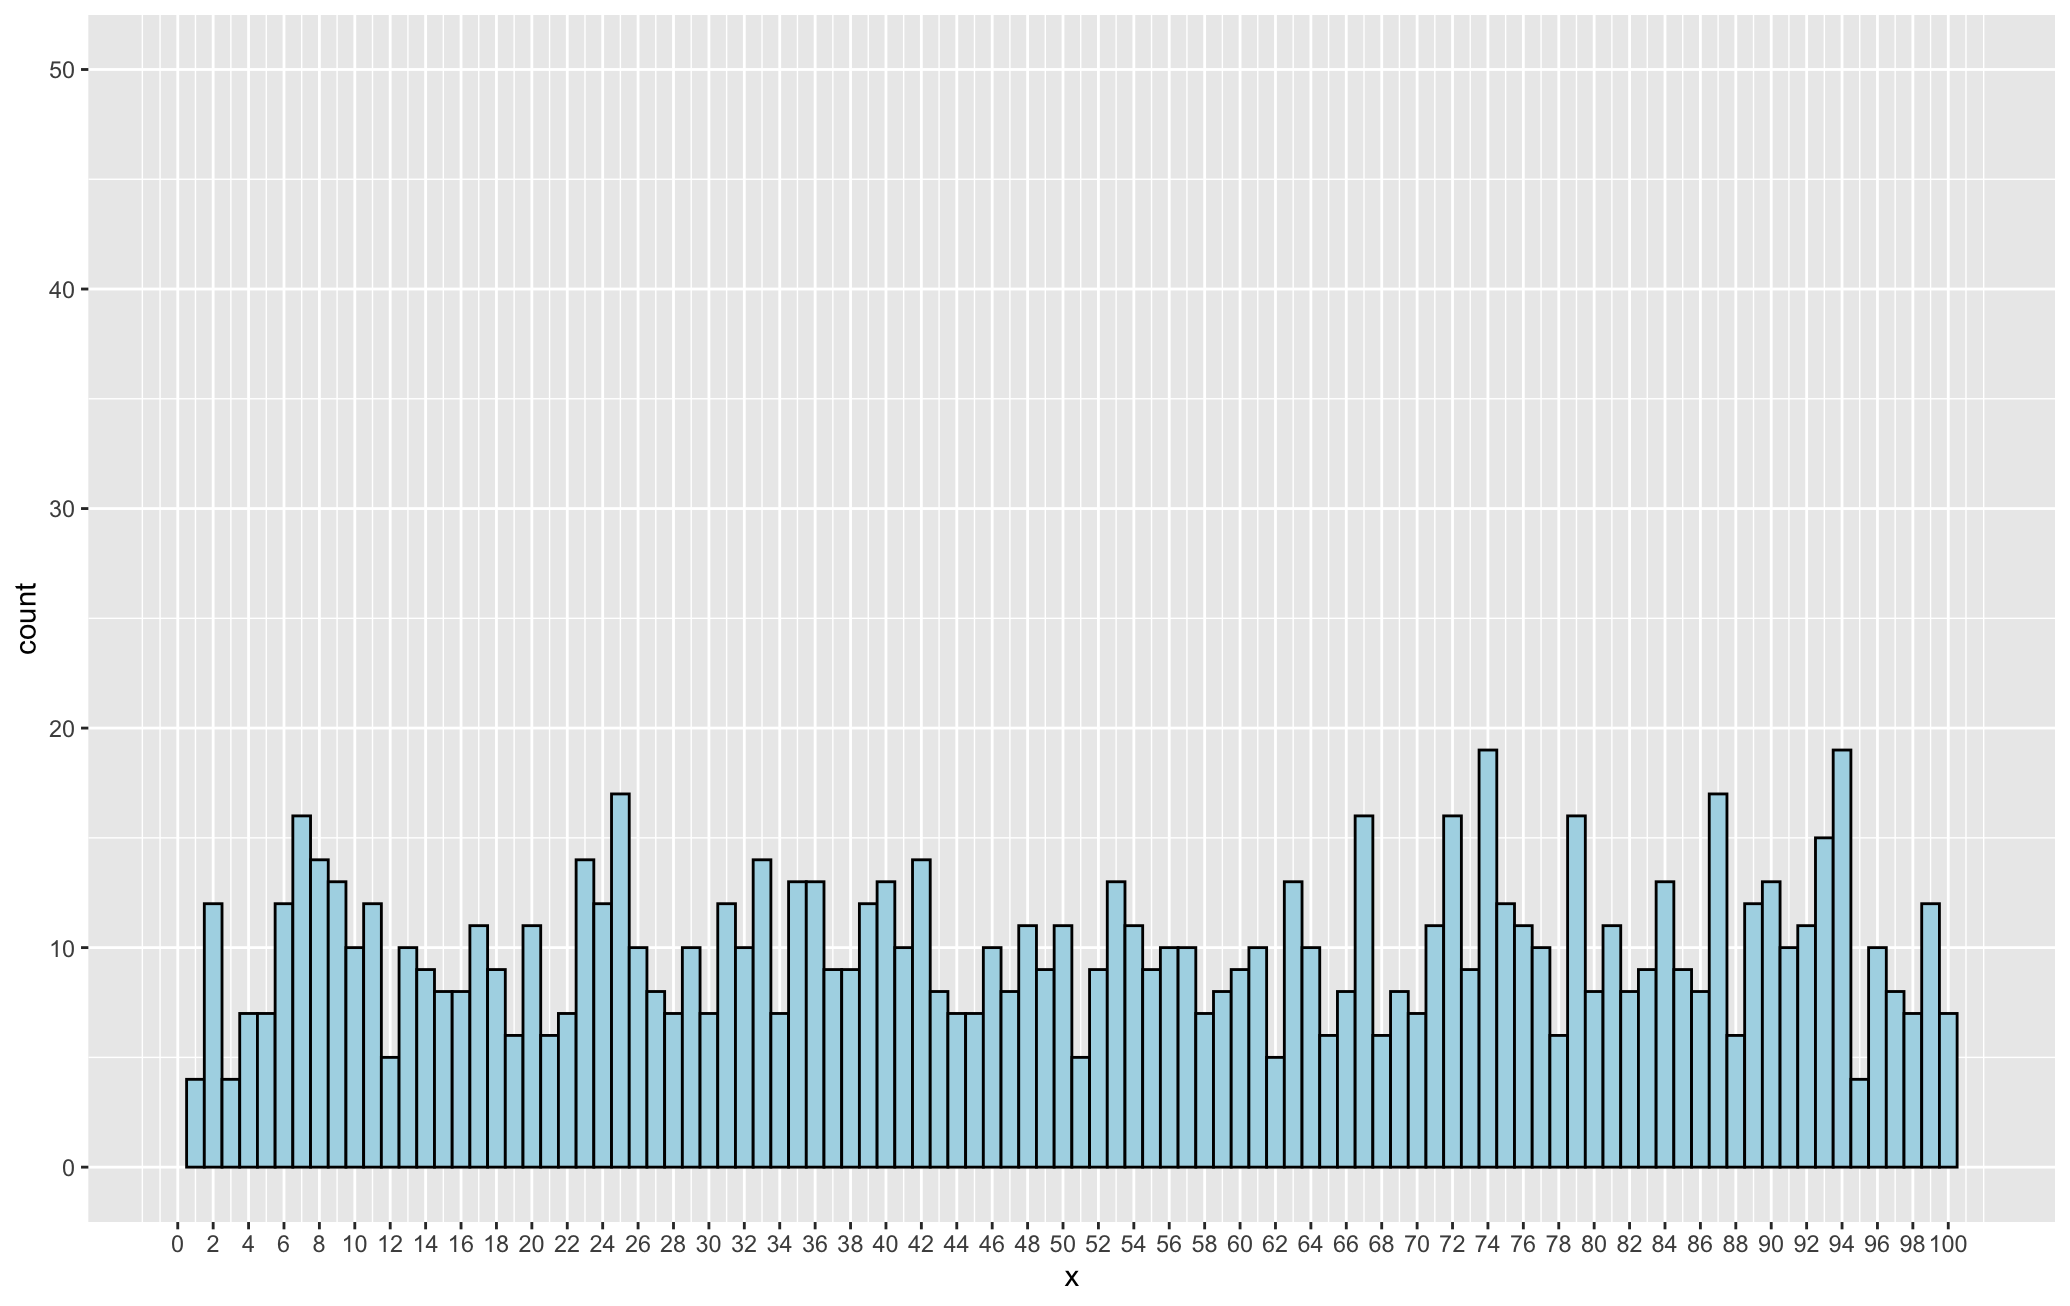
\includegraphics[width=0.7\linewidth,height=\textheight,keepaspectratio]{modules/02-variability/../../images/fig-approx-uniform-hist.png}

}

\caption{\label{fig-approx-uniform-hist}Approximate uniform distribution
-- each number between 1 and 100 occurs more or less the same number of
times}

\end{figure}%

A numerical variable does not necessarily have to be distributed
uniformly. That is each number in the range does not have to occur an
equal number of times exactly or approximately. We will now look at some
other common possibilities.

\begin{tcolorbox}[enhanced jigsaw, colback=white, leftrule=.75mm, toprule=.15mm, bottomtitle=1mm, breakable, coltitle=black, toptitle=1mm, title={Quick Check}, opacitybacktitle=0.6, colbacktitle=quarto-callout-note-color!10!white, arc=.35mm, left=2mm, colframe=quarto-callout-note-color-frame, titlerule=0mm, rightrule=.15mm, bottomrule=.15mm, opacityback=0]

Would you expect to find truly uniform distributions in real business
data??

\end{tcolorbox}

\begin{tcolorbox}[enhanced jigsaw, colback=white, leftrule=.75mm, toprule=.15mm, bottomtitle=1mm, breakable, coltitle=black, toptitle=1mm, title={Suggested answer}, opacitybacktitle=0.6, colbacktitle=quarto-callout-note-color!10!white, arc=.35mm, left=2mm, colframe=quarto-callout-note-color-frame, titlerule=0mm, rightrule=.15mm, bottomrule=.15mm, opacityback=0]

No.~Most business processes involve constraints, preferences, or natural
variation that cause some values to occur more often than others.

\end{tcolorbox}

\begin{tcolorbox}[enhanced jigsaw, colback=white, leftrule=.75mm, toprule=.15mm, bottomtitle=1mm, breakable, coltitle=black, toptitle=1mm, title={Quick Check}, opacitybacktitle=0.6, colbacktitle=quarto-callout-note-color!10!white, arc=.35mm, left=2mm, colframe=quarto-callout-note-color-frame, titlerule=0mm, rightrule=.15mm, bottomrule=.15mm, opacityback=0]

Give one business example where a roughly uniform distribution might
appear.

\end{tcolorbox}

\begin{tcolorbox}[enhanced jigsaw, colback=white, leftrule=.75mm, toprule=.15mm, bottomtitle=1mm, breakable, coltitle=black, toptitle=1mm, title={Suggested answer}, opacitybacktitle=0.6, colbacktitle=quarto-callout-note-color!10!white, arc=.35mm, left=2mm, colframe=quarto-callout-note-color-frame, titlerule=0mm, rightrule=.15mm, bottomrule=.15mm, opacityback=0]

Randomly assigned identification numbers (like school student ids) or
lottery numbers.

\end{tcolorbox}

\subsection{Bell shaped distributions}\label{bell-shaped-distributions}

Figure~\ref{fig-normal-low-sd-hist} and
Figure~\ref{fig-normal-higher-sd-hist} show two \emph{bell shaped}
distributions. Both have their peaks around the middle of the range
between 1 and 100. Which means that numbers closer to the middle -- or
closer to 50 -- occur more frequently than those far away from 50.

\begin{figure}

\centering{

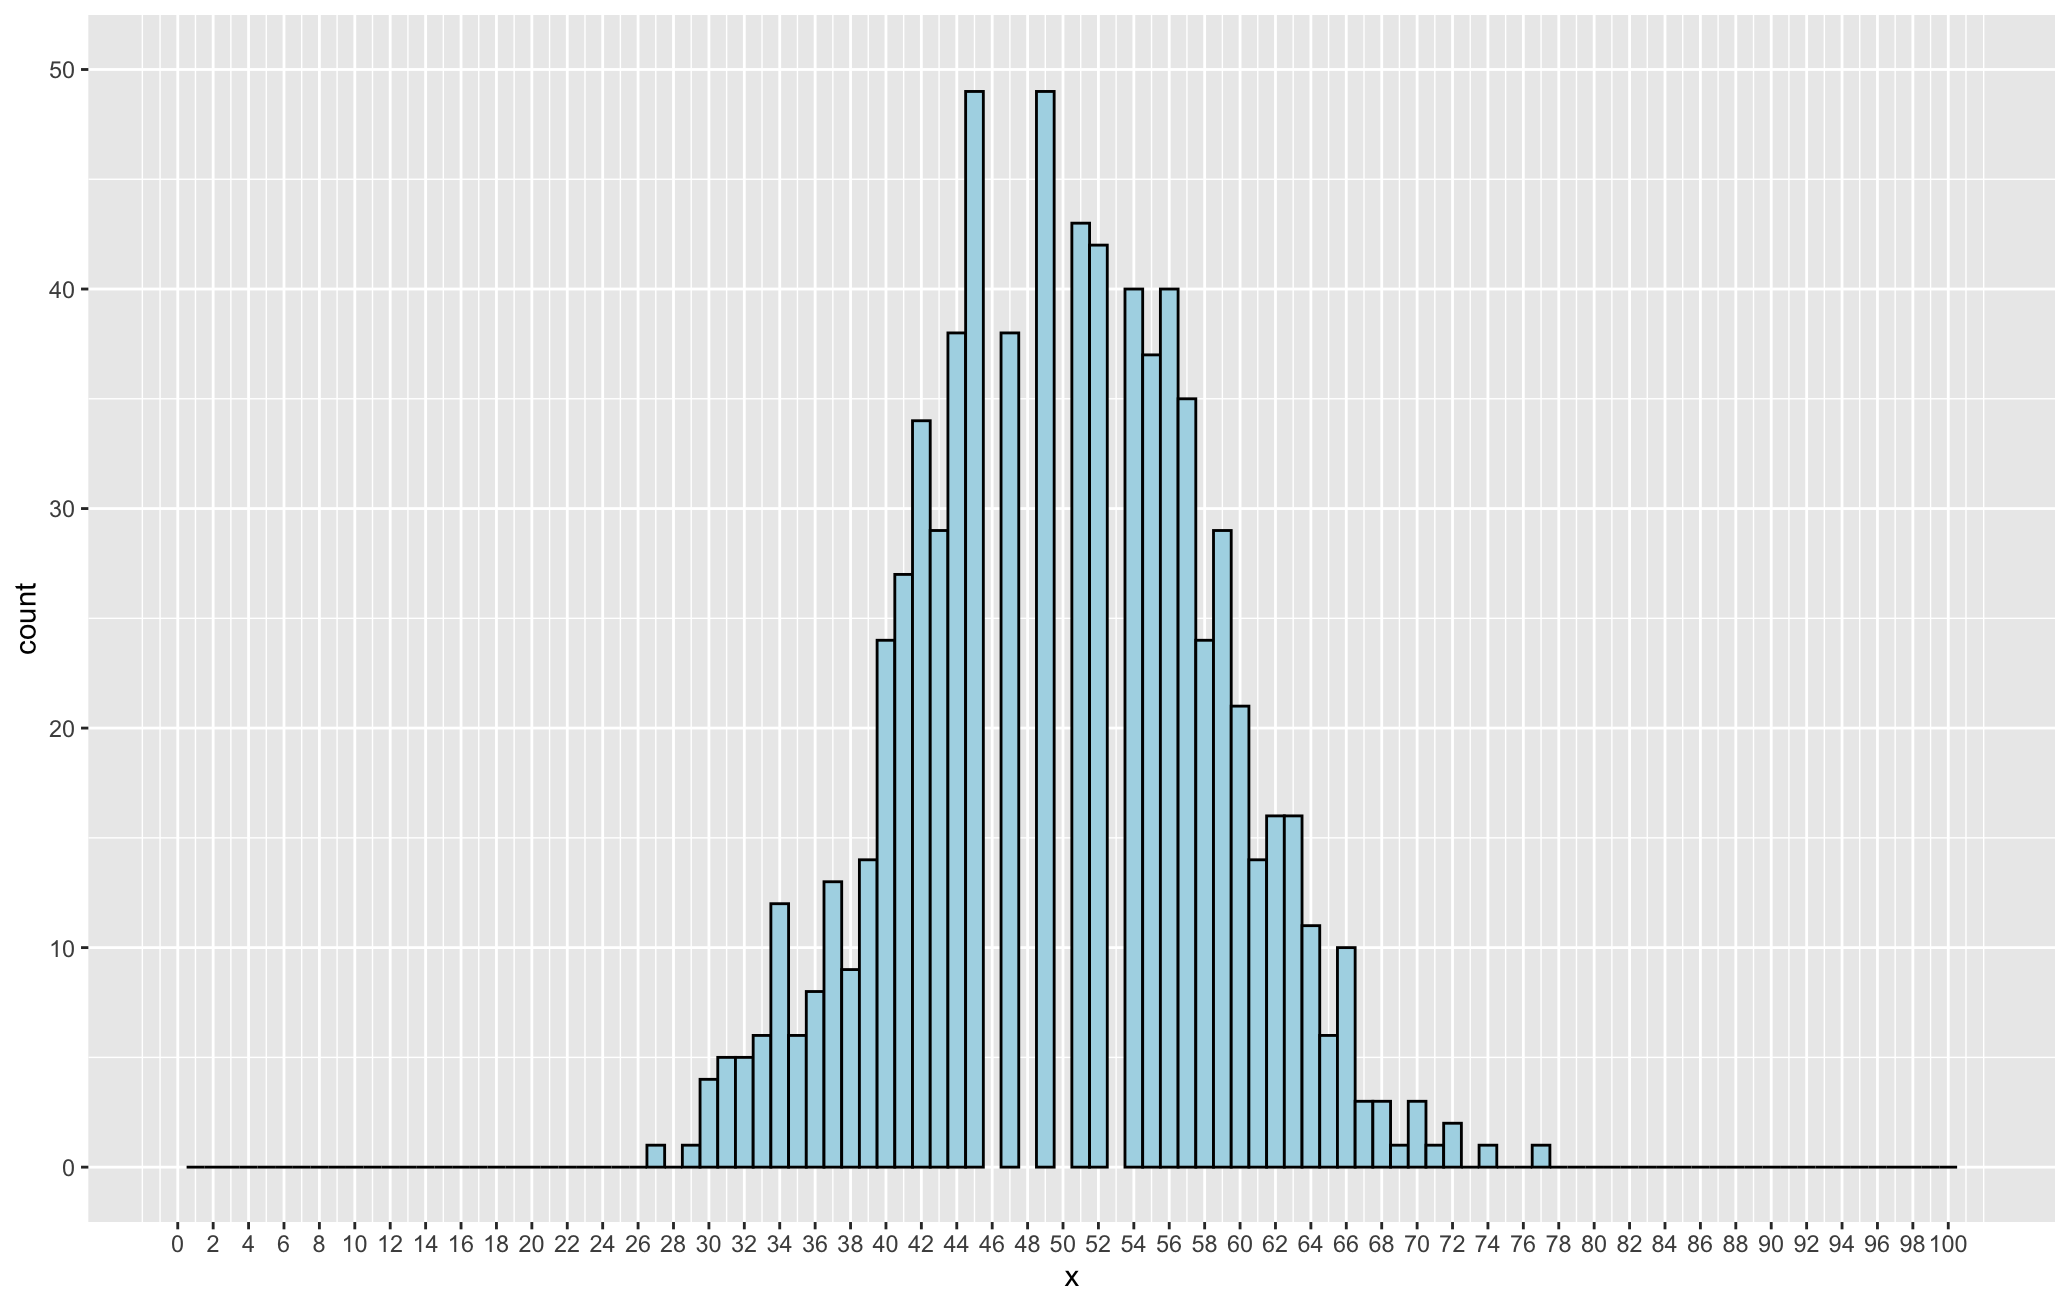
\includegraphics[width=0.7\linewidth,height=\textheight,keepaspectratio]{modules/02-variability/../../images/fig-normal-low-sd-hist.png}

}

\caption{\label{fig-normal-low-sd-hist}Symmetric bell shaped
distribution with a peak at around 50}

\end{figure}%

\begin{figure}

\centering{

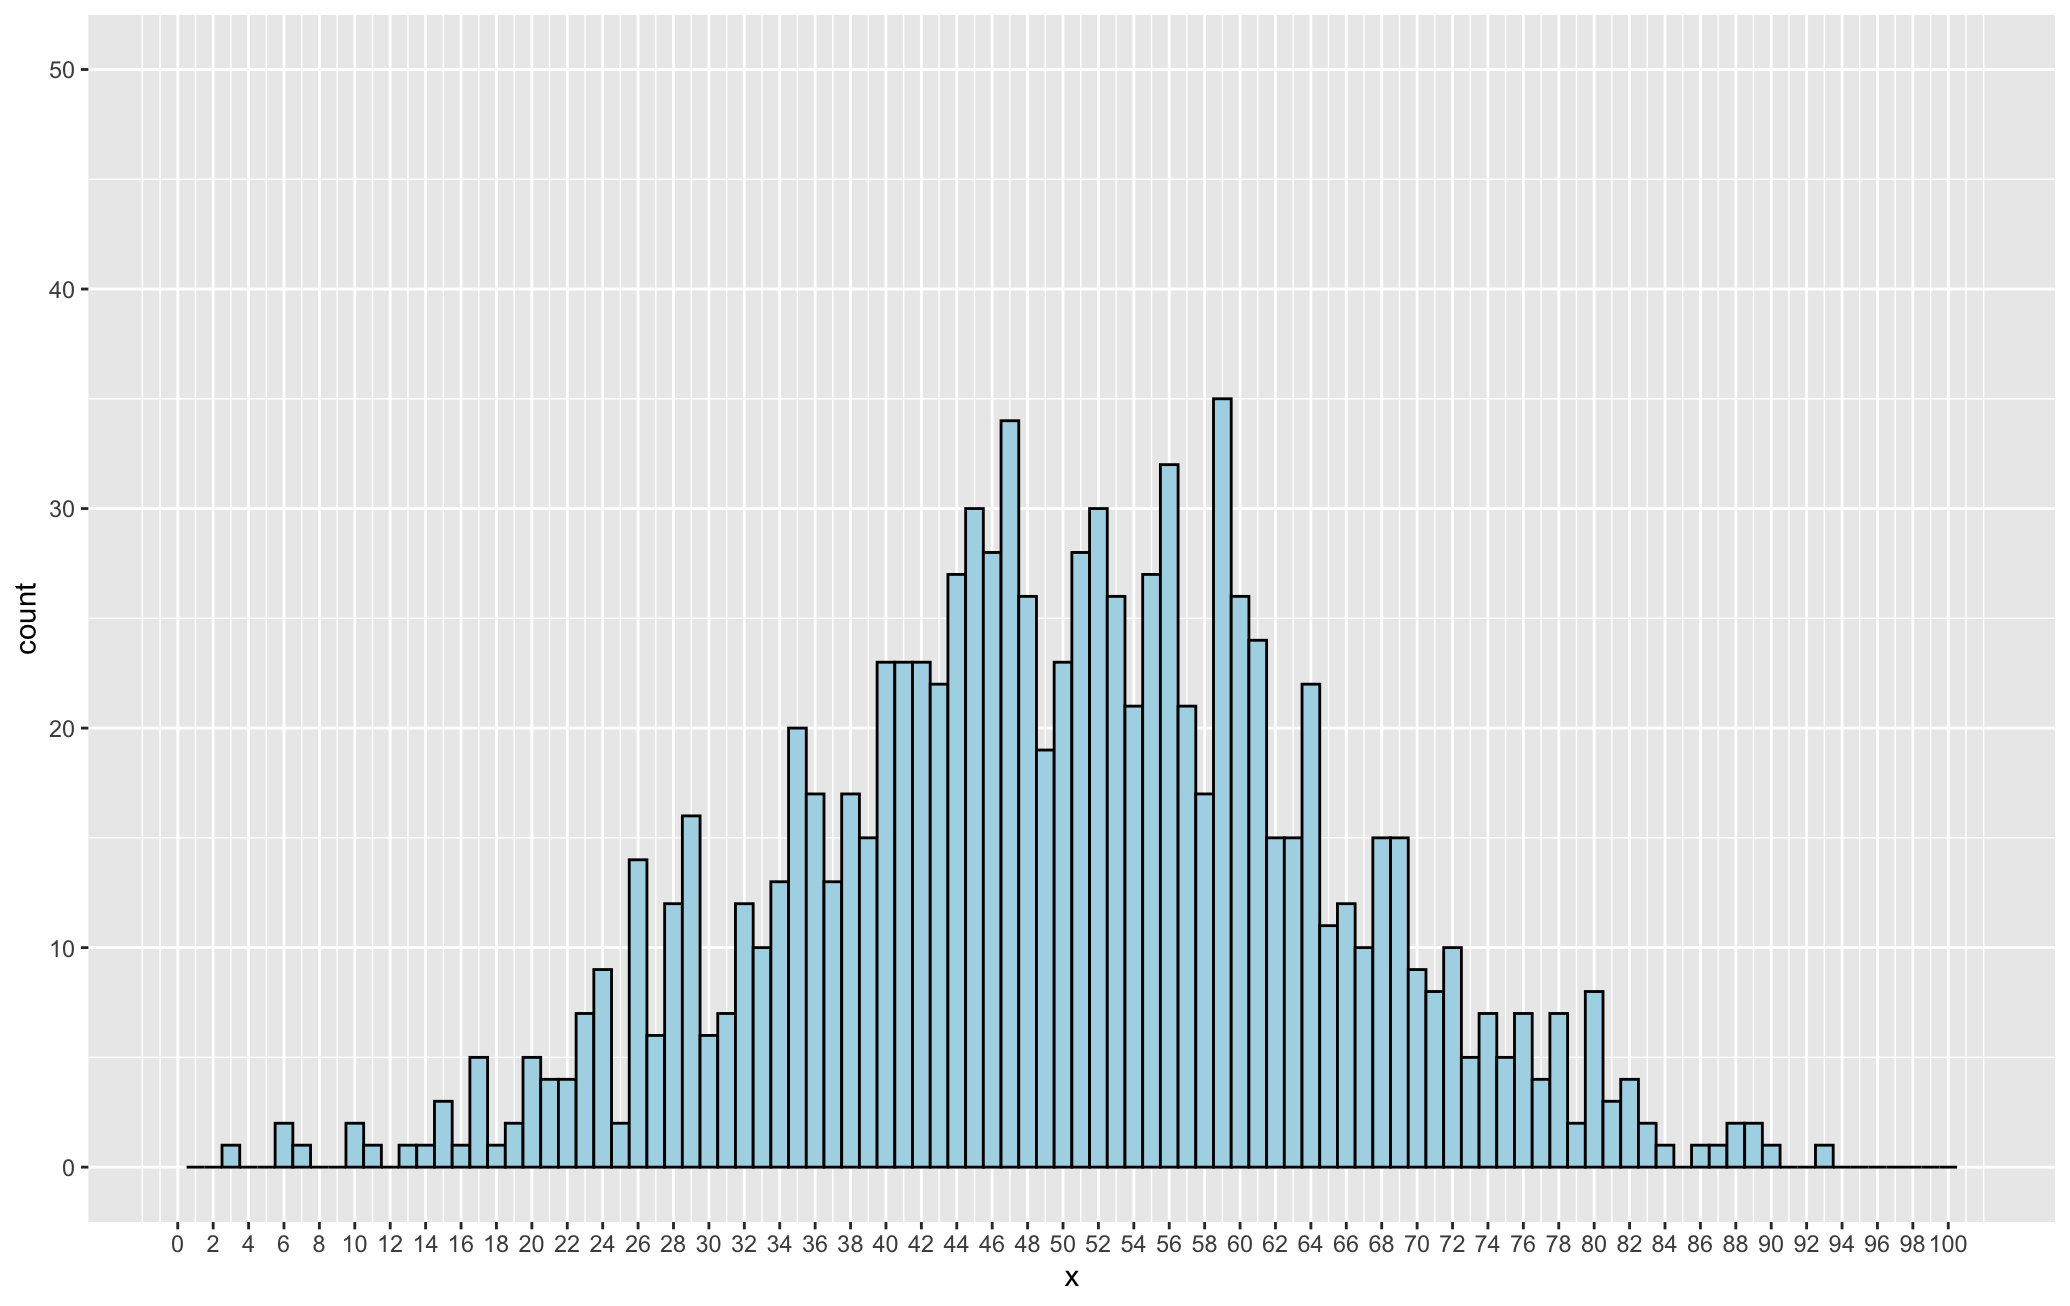
\includegraphics[width=0.7\linewidth,height=\textheight,keepaspectratio]{modules/02-variability/../../images/fig-normal-higher-sd-hist.png}

}

\caption{\label{fig-normal-higher-sd-hist}Symmetric bell shaped
distribution with a peak at around 50 and higher spread than in
Figure~\ref{fig-normal-low-sd-hist}}

\end{figure}%

Both Figure~\ref{fig-normal-low-sd-hist} and
Figure~\ref{fig-normal-higher-sd-hist} show bell shaped distributions
that are also symmetric. That is, the shape to the left of the peak is
approximately similar to the shape on the right.

So, both of these are bell shaped and symmetric, and yet they are
obviously different? Can you describe how they are different?

We see that the spread* of the numbers is quite different. In
Figure~\ref{fig-normal-low-sd-hist} the numbers are more concentrated
near the middle than is the case in
Figure~\ref{fig-normal-higher-sd-hist}. Consequently, the peak in the
first figure is higher. For example, the numbers 47 and 51 occur nearly
50 times. In Figure~\ref{fig-normal-higher-sd-hist}, the highest
frequency is around 35. We call the ends of the bell shape as
\emph{tails}. We see that Figure~\ref{fig-normal-higher-sd-hist} has
\emph{fatter} tails.

We have seen three different possibilities for how a set of 1000 numbers
in the range 1 to 100 can be distributed. Even though the averages of a
set of numbers and even their range might be the same they can still be
\emph{distributed} very differently.

\subsection{Multi-modal distributions}\label{multi-modal-distributions}

In Figure~\ref{fig-normal-low-sd-hist} and
Figure~\ref{fig-normal-higher-sd-hist} we saw distributions that each
had a single peak. This does not have to be the case. shows a case where
we have two peaks.

\begin{figure}

\centering{

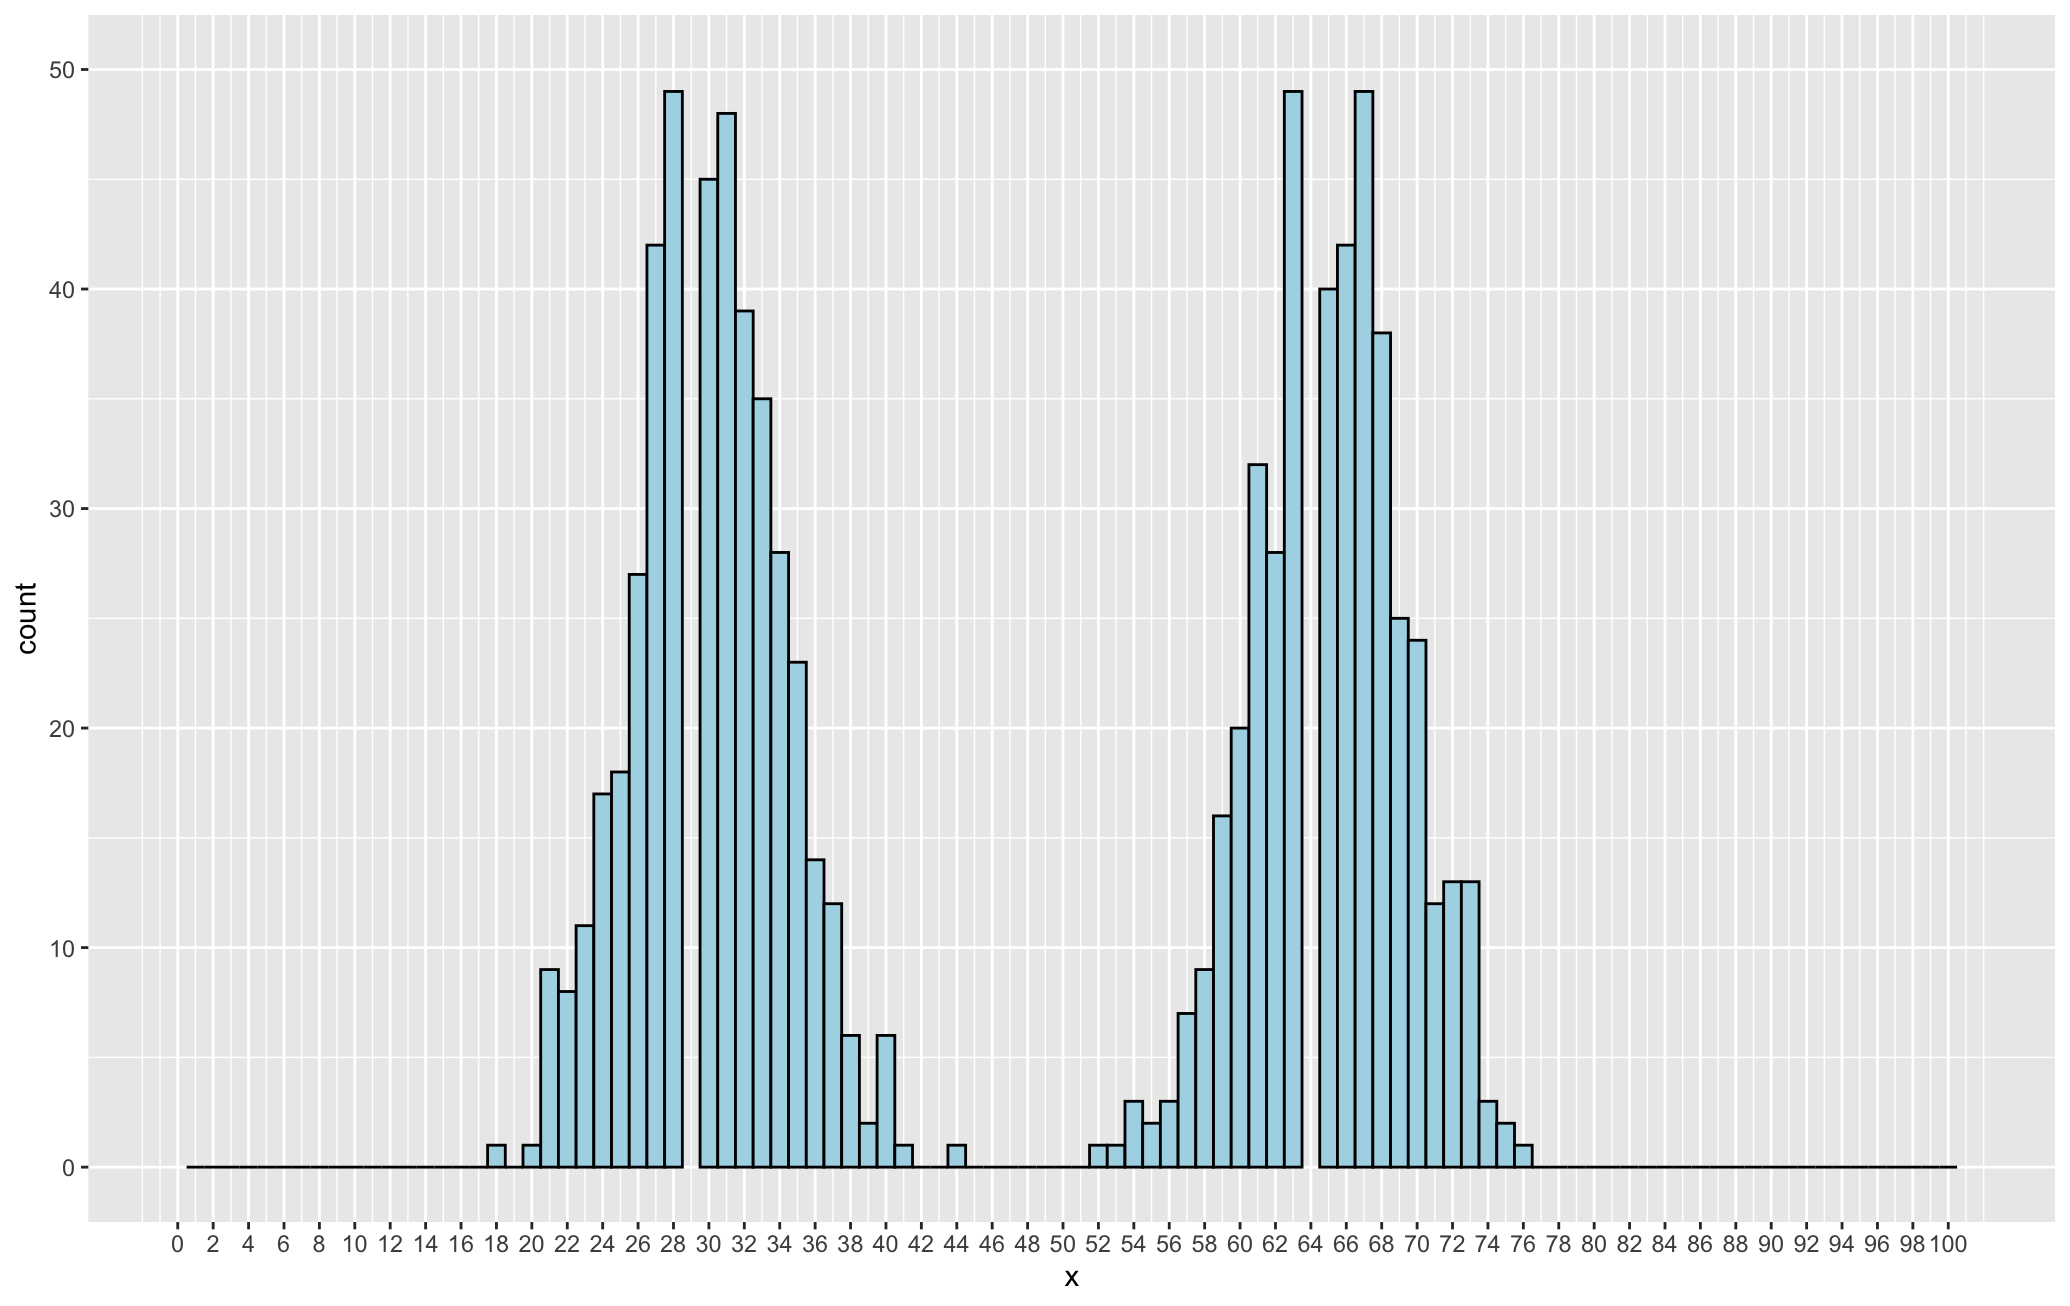
\includegraphics[width=0.7\linewidth,height=\textheight,keepaspectratio]{modules/02-variability/../../images/fig-bimodal-hist.png}

}

\caption{\label{fig-bimodal-hist}Distribution with more than one peak --
multi-modal distribution}

\end{figure}%

\subsection{Skewed distributions}\label{skewed-distributions}

Thus far, we have seen distributions in which the shape has always been
symmetric -- explicitly so in the bell-shaped examples, but also true
for the \emph{uniform} examples. Figure~\ref{fig-right-skew-hist} and
Figure~\ref{fig-left-skew-hist} show examples of asymmetric
distributions. The first has a long \emph{tail} on the right and is said
to be \emph{right-skewed} and the second has its \emph{tail} on the left
and is said to be \emph{left-skewed}.

\begin{figure}

\centering{

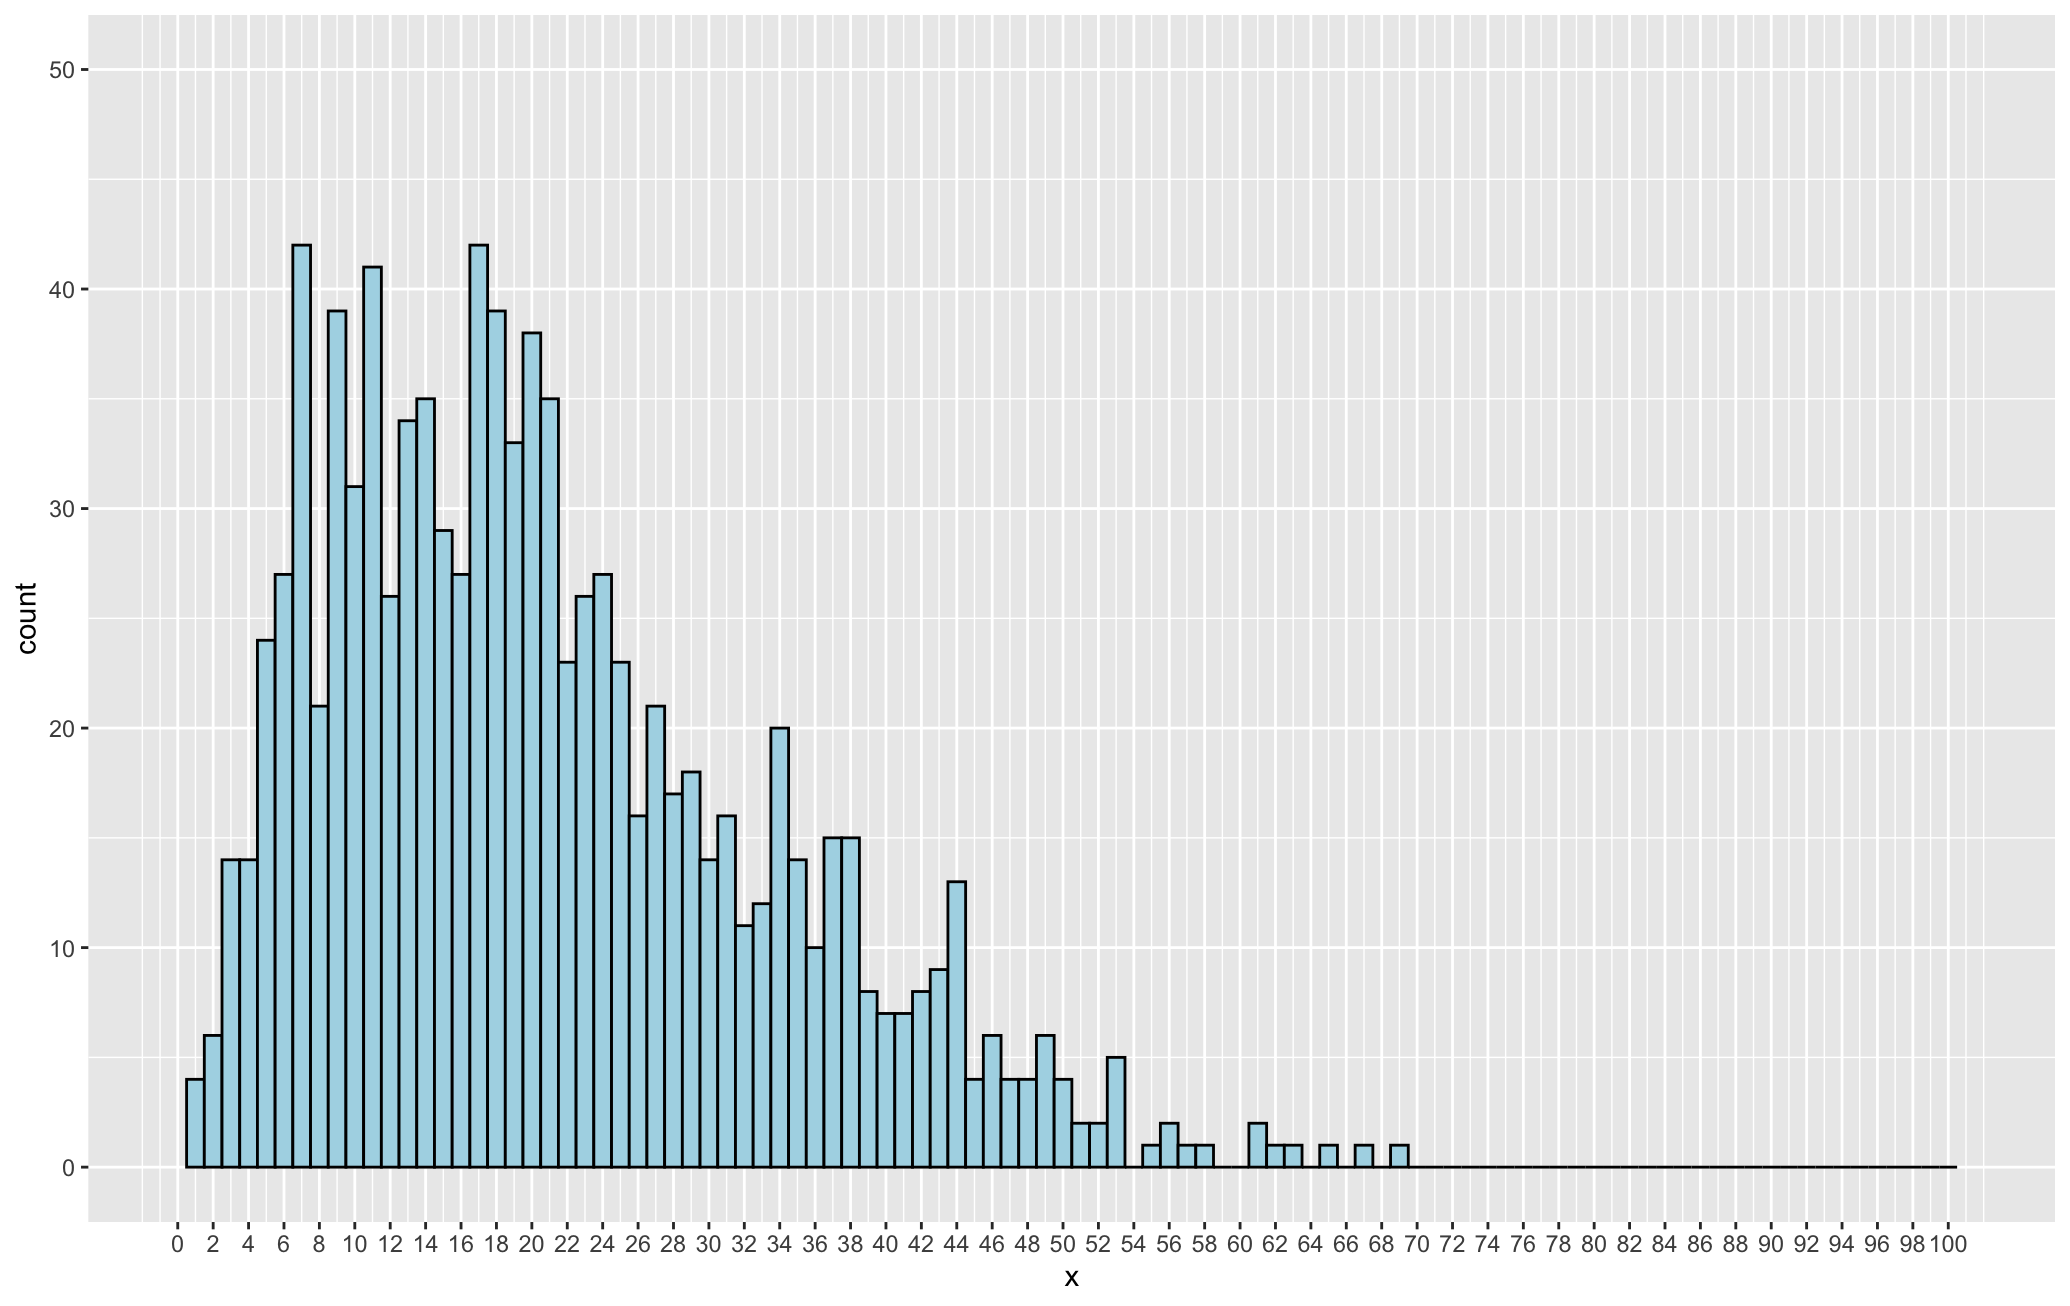
\includegraphics[width=0.7\linewidth,height=\textheight,keepaspectratio]{modules/02-variability/../../images/fig-right-skew-hist.png}

}

\caption{\label{fig-right-skew-hist}Asymmetric distribution with a right
skew}

\end{figure}%

\begin{figure}

\centering{

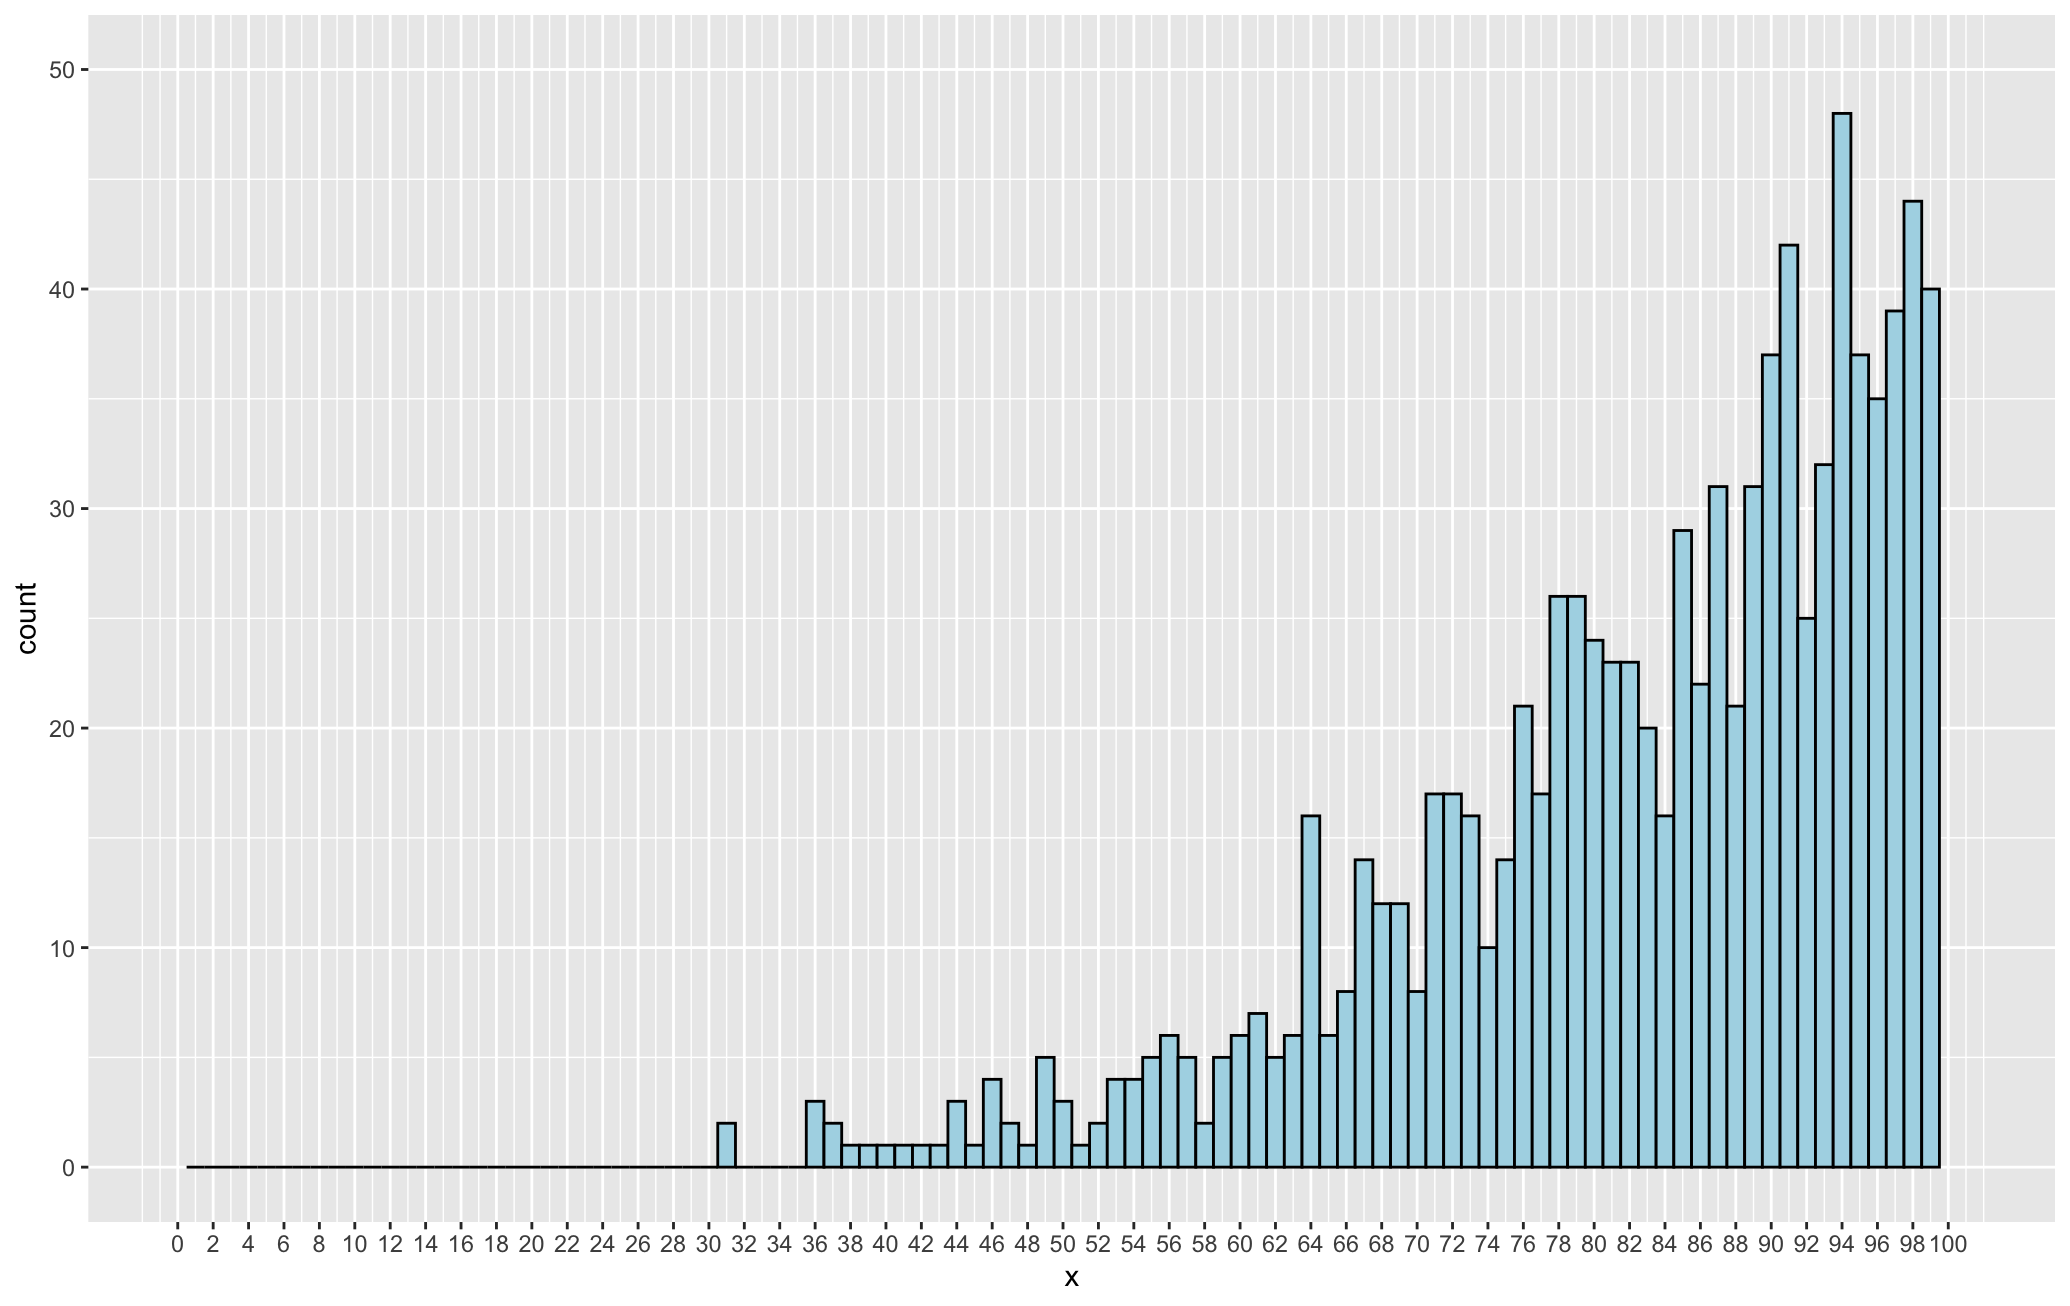
\includegraphics[width=0.7\linewidth,height=\textheight,keepaspectratio]{modules/02-variability/../../images/fig-left-skew-hist.png}

}

\caption{\label{fig-left-skew-hist}Asymmetric distribution with a left
skew}

\end{figure}%

\section{Violin plots}\label{violin-plots}

Now that we have clarified the idea of a \emph{distribution} let us look
at distributions of numerical variables through \emph{violin} plots.
These plots serve the same function as the histograms we have looked at
in the previous section, but we can do more.

\begin{quote}
A violin plot is not a new idea. It is a different lens on the same
distribution concepts you already saw in the previous section.
\end{quote}

Let us start off by looking at a violin plot of the variable
\emph{minutes} from the \emph{Boston\_marathon} data frame

\begin{lstlisting}[language=R]
Boston_marathon |> 
  point_plot(minutes ~ 1, annot = "violin")
\end{lstlisting}

\begin{figure}[H]

\centering{

\pandocbounded{
\includegraphics[keepaspectratio]{modules/02-variability/violin-plots_files/figure-pdf/fig-boston-marathon-minutes-violin-1.pdf}}

}

\caption{\label{fig-boston-marathon-minutes-violin}Violin plot of the
\emph{minutes} variable from the \emph{Boston\_marathon} data frame}

\end{figure}%

The width of the violin at any point on the y-axis shows the
\textbf{relative frequency} of data values close to that point. The
widest part of the violin occurs at around 145 minutes. This means that
the maximum concentration of winning times in the data set is close to
145 minutes. The plot does not tell us exactly what the frequency is.
The width only shows the relative frequency. Looking at where the violin
is very narrow, we can say that very few runners took more than 175
minutes to complete the race. Also, relatively low numbers of people
took less than about 125 minutes. We can see a higher density of points
around the broad regions of the violin and a low density in the narrow
areas of the violin.

\begin{tcolorbox}[enhanced jigsaw, colback=white, leftrule=.75mm, toprule=.15mm, bottomtitle=1mm, breakable, coltitle=black, toptitle=1mm, title=\textcolor{quarto-callout-warning-color}{\faExclamationTriangle}\hspace{0.5em}{Important:}, opacitybacktitle=0.6, colbacktitle=quarto-callout-warning-color!10!white, arc=.35mm, left=2mm, colframe=quarto-callout-warning-color-frame, titlerule=0mm, rightrule=.15mm, bottomrule=.15mm, opacityback=0]

The width of a violin \textbf{does not represent the number of
observations at an exact value}. It represents a \textbf{smoothed
estimate} of how densely values occur near that value as compared to the
density of values near other values.

\end{tcolorbox}

\subsection{Elements of the plot}\label{elements-of-the-plot}

Until now, the plots we have generated using \emph{point plot} have only
shown the actual points. However, in
Figure~\ref{fig-boston-marathon-minutes-violin} we see two distinct
elements:

\begin{itemize}
\tightlist
\item
  a jittered plot of the individual points
\item
  a violin-shaped solid area -- an \emph{annotation} encompassing the
  points themselves
\end{itemize}

The points represent the raw data and the violin adds an
\emph{annotation} that interprets the data in some way. Here, the
interpretation is a violin plot that helps us visualize the distribution
of the values.

\subsection{Examining the code}\label{examining-the-code}

We examine the code now. In the code for
Figure~\ref{fig-boston-marathon-minutes-violin}, we can see two
arguments for the \emph{point\_plot} function. The first argument
specifies the tilde expression mapping the axes. The second specifies
the type of \emph{annotation} we want.
Figure~\ref{fig-boston-marathon-minutes-violin-code-dissect} shows the
code with the two arguments labeled.

\begin{figure}

\centering{

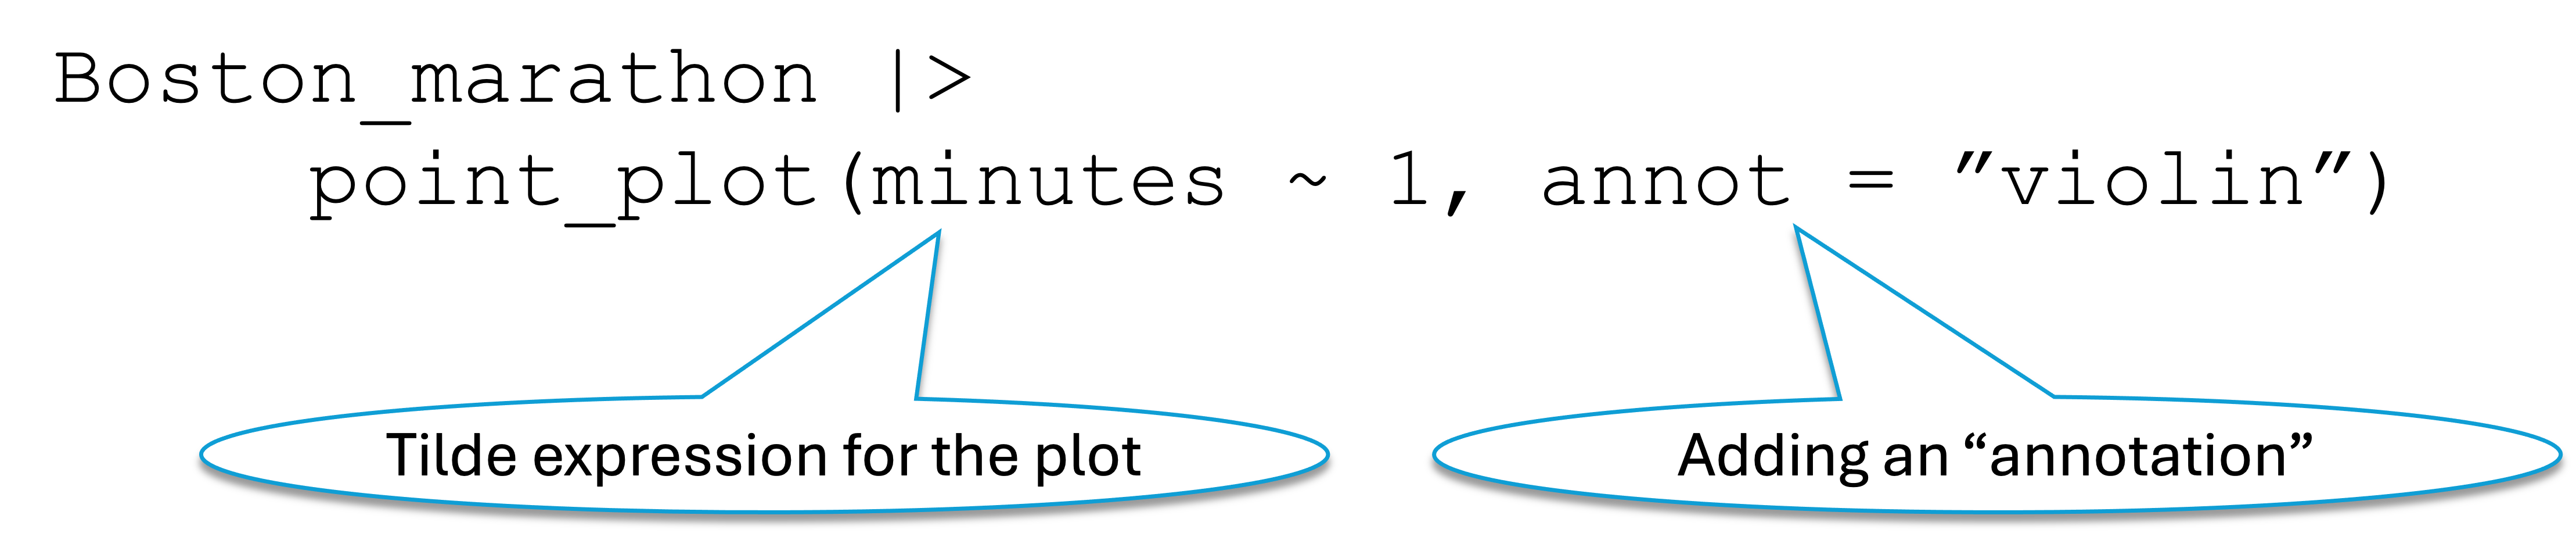
\includegraphics[width=0.7\linewidth,height=\textheight,keepaspectratio]{modules/02-variability/../../images/fig-boston-marathon-minutes-violin-code-dissect.png}

}

\caption{\label{fig-boston-marathon-minutes-violin-code-dissect}The code
to generate Figure~\ref{fig-boston-marathon-minutes-violin} passes two
arguments to the \emph{point\_plot} function -- a tilde expression and
an \emph{annotation} specification}

\end{figure}%

Figure~\ref{fig-tilde-expression-violin-boston-marathon} explains the
tilde expression used for the plot. Mapping of \emph{minutes} to the
y-axis conforms to what we did before. This plot deals with just a
single variable -- we have no variable on the x-axis. When there is no
variable on the x-axis, we conventionally that by just using ``1'' for
the x-axis variable.

\begin{figure}

\centering{

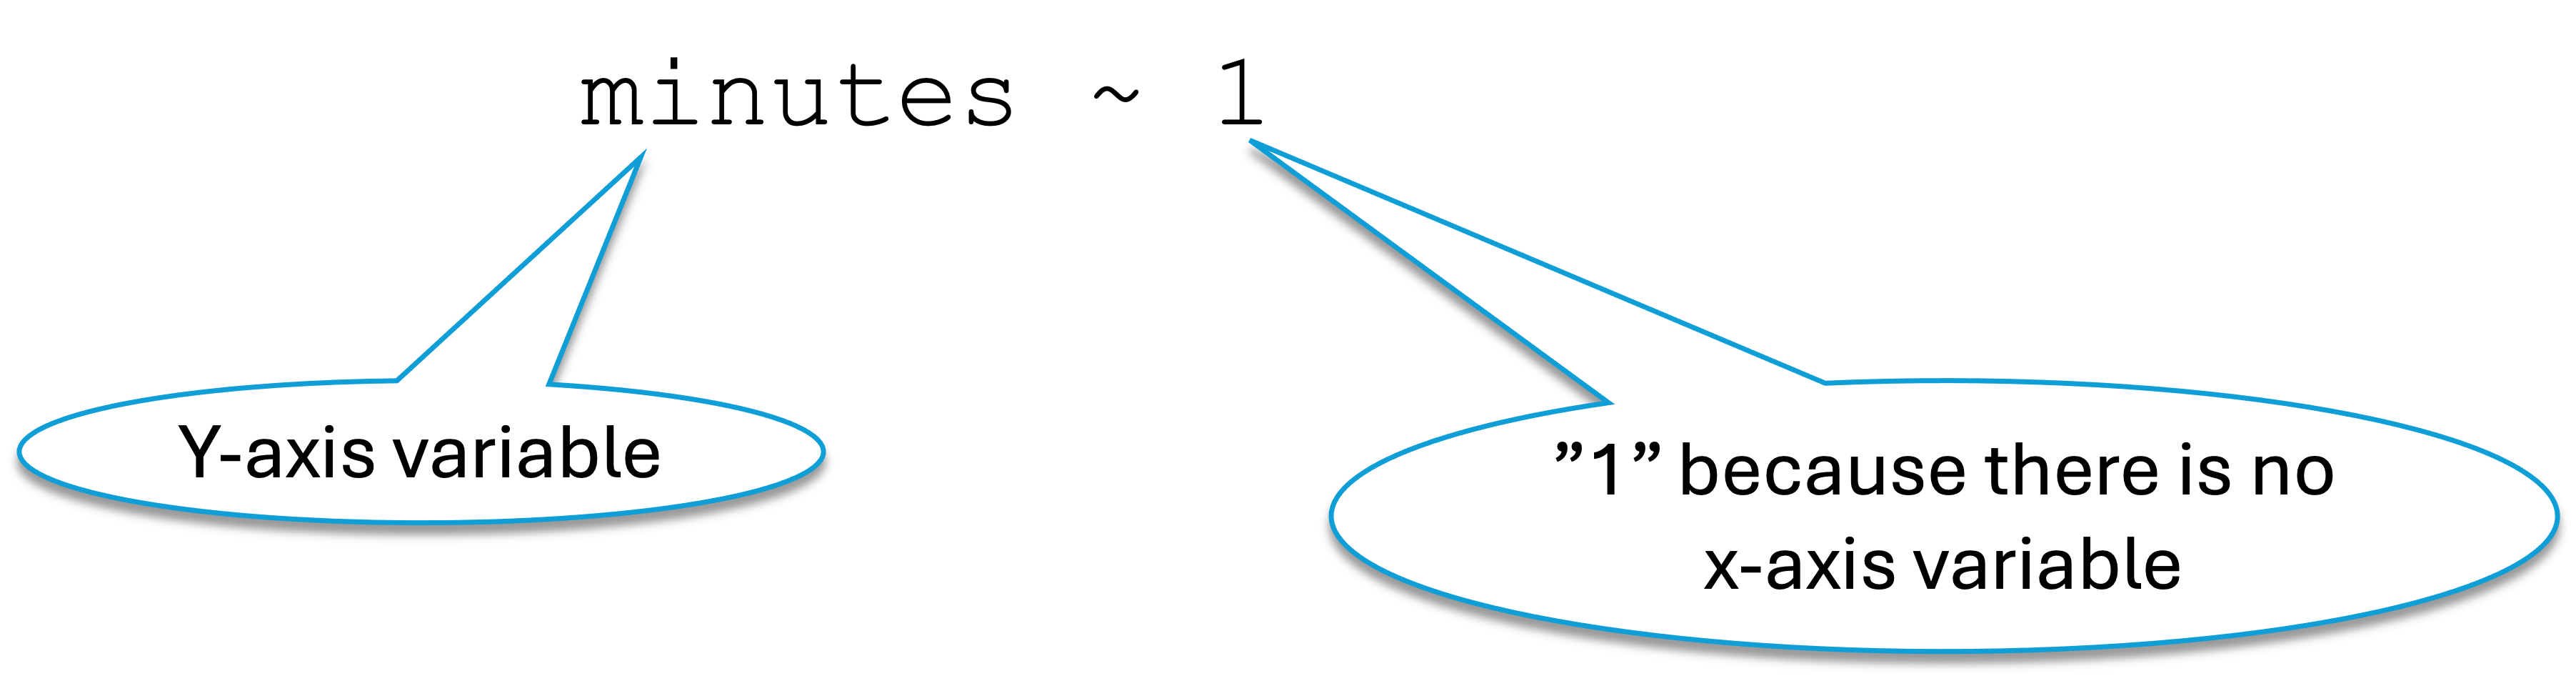
\includegraphics[width=0.7\linewidth,height=\textheight,keepaspectratio]{modules/02-variability/../../images/fig-tilde-expression-violin-boston-marathon.png}

}

\caption{\label{fig-tilde-expression-violin-boston-marathon}The tilde
expression of
Figure~\ref{fig-boston-marathon-minutes-violin-code-dissect} we place
\emph{minutes} on the y-axis and since the x-axis has no variable, we
just state ``1''}

\end{figure}%

Figure~\ref{fig-annot-violin-argument} explains the second argument in
generating a \emph{violin plot}.

\begin{figure}

\centering{

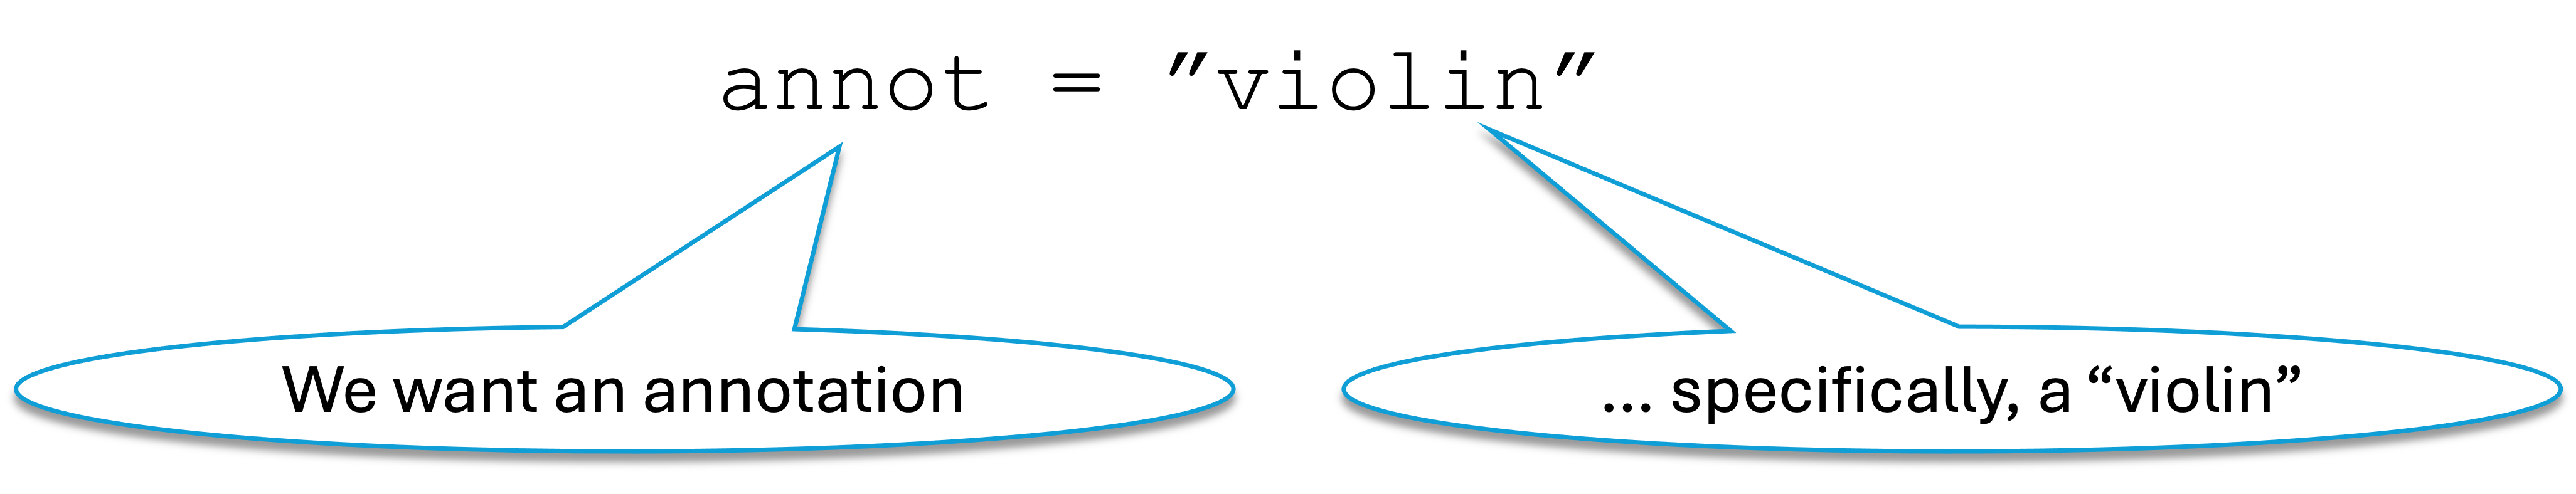
\includegraphics[width=0.7\linewidth,height=\textheight,keepaspectratio]{modules/02-variability/../../images/fig-annot-violin-argument.png}

}

\caption{\label{fig-annot-violin-argument}We specify that we want a
\emph{violin annotation}}

\end{figure}%

\section{Violin plots and distribution
shapes}\label{violin-plots-and-distribution-shapes}

The violin plot displays vertical reflectional symmetry. We can get all
the information that the plot conveys just by slicing the plot
vertically down the middle and looking at either of the two chunks.

When we first talked about the various distribution shapes like
\emph{uniform}, \emph{symmetric bell-shaped}, and \emph{skewed}, we used
histograms to convey the ideas. We can deduce the same information from
violin plots as well. In the next section, we will see a few more
examples. We will discuss distribution shapes in the context of those
examples.

\begin{tcolorbox}[enhanced jigsaw, colback=white, leftrule=.75mm, toprule=.15mm, bottomtitle=1mm, breakable, coltitle=black, toptitle=1mm, title=\textcolor{quarto-callout-tip-color}{\faLightbulb}\hspace{0.5em}{What to look for in a violin plot}, opacitybacktitle=0.6, colbacktitle=quarto-callout-tip-color!10!white, arc=.35mm, left=2mm, colframe=quarto-callout-tip-color-frame, titlerule=0mm, rightrule=.15mm, bottomrule=.15mm, opacityback=0]

\begin{itemize}
\tightlist
\item
  Where are most values concentrated?
\item
  Are there one or multiple peaks?
\item
  Is the distribution symmetric or skewed?
\item
  Are there long tails or unusual shapes?
\end{itemize}

\end{tcolorbox}

\subsection{More examples}\label{more-examples}

We see a few more examples to reinforce the idea.
Figure~\ref{fig-price-violin-from-price-demand-dataframe} shows a violin
plot of the variable \emph{price} from the \emph{price\_demand} data
frame.

\begin{lstlisting}[language=R]
price_demand |> 
  point_plot(price ~ 1, annot = "violin")
\end{lstlisting}

\begin{figure}[H]

\centering{

\pandocbounded{
\includegraphics[keepaspectratio]{modules/02-variability/violin-plots_files/figure-pdf/fig-price-violin-from-price-demand-dataframe-1.pdf}}

}

\caption{\label{fig-price-violin-from-price-demand-dataframe}Violin plot
of the \emph{price} variable from the \emph{price\_demand} data frame}

\end{figure}%

If we look at only the left or right half of
Figure~\ref{fig-price-violin-from-price-demand-dataframe}, turn it right
by 90 degrees and get rid of the display of the individual points, we
get Figure~\ref{fig-sliced-rotated-violin} -- a symmetric bell-shaped
distribution.

\begin{figure}

\centering{

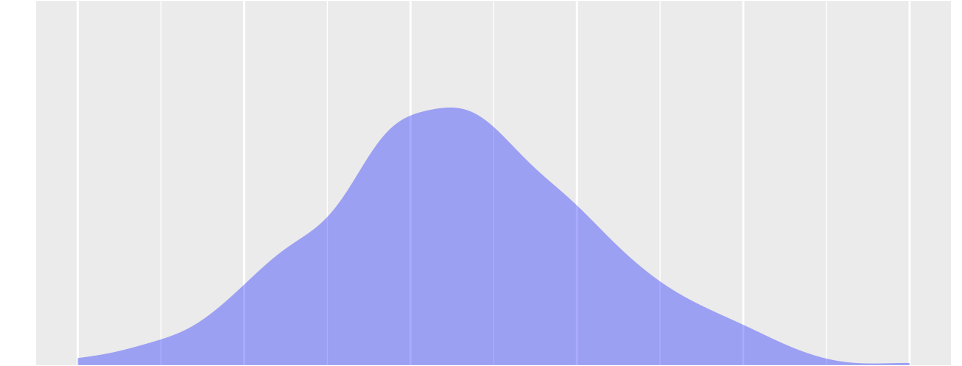
\includegraphics[width=0.7\linewidth,height=\textheight,keepaspectratio]{modules/02-variability/../../images/fig-sliced-rotated-violin.png}

}

\caption{\label{fig-sliced-rotated-violin}Violin from
Figure~\ref{fig-price-violin-from-price-demand-dataframe} split and
rotated 90 degrees right to reveal the distribution in the form we had
seen before}

\end{figure}%

Figure~\ref{fig-balance-violin-from-acct-type-balance-dataframe} shows a
violin plot of the \emph{balance} variable from the
\emph{acct\_type\_balance} data frame.

\begin{lstlisting}[language=R]
acct_type_balance |> 
  point_plot(balance ~ 1, annot = "violin")
\end{lstlisting}

\begin{figure}[H]

\centering{

\pandocbounded{
\includegraphics[keepaspectratio]{modules/02-variability/violin-plots_files/figure-pdf/fig-balance-violin-from-acct-type-balance-dataframe-1.pdf}}

}

\caption{\label{fig-balance-violin-from-acct-type-balance-dataframe}Violin
plot of the \emph{balance} variable from the \emph{acct\_type\_balance}
data frame}

\end{figure}%

We can see from
Figure~\ref{fig-price-violin-from-price-demand-dataframe} that
\emph{price} is bell-shaped and unimodal,but not symmetric. It is skewed
towards the lower values because the tail is at the bottom. If we slice
and rotate it as before then we would say that it is skewed left.

Next we look at the distribution of \emph{advertising\_spend\_k} from
the \emph{advertising\_sales\_channel} data frame.
Figure~\ref{fig-advertising-spend-violin-from-advertising-sales-channel-dataframe}
shows the violin plot. From it we see that \emph{advertising\_spend\_k}
follows a nearly uniform distribution, but not perfectly so. It is
mildly bi modal.

\begin{lstlisting}[language=R]
advertising_sales_channel |> 
  point_plot(advertising_spend_k ~ 1, annot = "violin")
\end{lstlisting}

\begin{figure}[H]

\centering{

\pandocbounded{
\includegraphics[keepaspectratio]{modules/02-variability/violin-plots_files/figure-pdf/fig-advertising-spend-violin-from-advertising-sales-channel-dataframe-1.pdf}}

}

\caption{\label{fig-advertising-spend-violin-from-advertising-sales-channel-dataframe}Violin
plot of the \emph{advertising\_spend\_k} variable from the
\emph{advertising\_sales\_channel} data frame}

\end{figure}%

\begin{tcolorbox}[enhanced jigsaw, colback=white, leftrule=.75mm, toprule=.15mm, bottomtitle=1mm, breakable, coltitle=black, toptitle=1mm, title={Quick Check}, opacitybacktitle=0.6, colbacktitle=quarto-callout-note-color!10!white, arc=.35mm, left=2mm, colframe=quarto-callout-note-color-frame, titlerule=0mm, rightrule=.15mm, bottomrule=.15mm, opacityback=0]

Where would the violin be widest for a symmetric bell-shaped
distribution?

\end{tcolorbox}

\begin{tcolorbox}[enhanced jigsaw, colback=white, leftrule=.75mm, toprule=.15mm, bottomtitle=1mm, breakable, coltitle=black, toptitle=1mm, title={Suggested answer}, opacitybacktitle=0.6, colbacktitle=quarto-callout-note-color!10!white, arc=.35mm, left=2mm, colframe=quarto-callout-note-color-frame, titlerule=0mm, rightrule=.15mm, bottomrule=.15mm, opacityback=0]

Near the center, where values occur most frequently.

\end{tcolorbox}

\begin{tcolorbox}[enhanced jigsaw, colback=white, leftrule=.75mm, toprule=.15mm, bottomtitle=1mm, breakable, coltitle=black, toptitle=1mm, title={Quick Check}, opacitybacktitle=0.6, colbacktitle=quarto-callout-note-color!10!white, arc=.35mm, left=2mm, colframe=quarto-callout-note-color-frame, titlerule=0mm, rightrule=.15mm, bottomrule=.15mm, opacityback=0]

If you have a symmetric bell-shaped violin plot what does it say about
values on the high and low ends of the range?

\end{tcolorbox}

\begin{tcolorbox}[enhanced jigsaw, colback=white, leftrule=.75mm, toprule=.15mm, bottomtitle=1mm, breakable, coltitle=black, toptitle=1mm, title={Suggested answer}, opacitybacktitle=0.6, colbacktitle=quarto-callout-note-color!10!white, arc=.35mm, left=2mm, colframe=quarto-callout-note-color-frame, titlerule=0mm, rightrule=.15mm, bottomrule=.15mm, opacityback=0]

Extreme high and low values occur with similar rarity.

\end{tcolorbox}

\begin{tcolorbox}[enhanced jigsaw, colback=white, leftrule=.75mm, toprule=.15mm, bottomtitle=1mm, breakable, coltitle=black, toptitle=1mm, title={Quick Check}, opacitybacktitle=0.6, colbacktitle=quarto-callout-note-color!10!white, arc=.35mm, left=2mm, colframe=quarto-callout-note-color-frame, titlerule=0mm, rightrule=.15mm, bottomrule=.15mm, opacityback=0]

Would you generally expect bell-shaped distributions in measurement
based data?

\end{tcolorbox}

\begin{tcolorbox}[enhanced jigsaw, colback=white, leftrule=.75mm, toprule=.15mm, bottomtitle=1mm, breakable, coltitle=black, toptitle=1mm, title={Suggested answer}, opacitybacktitle=0.6, colbacktitle=quarto-callout-note-color!10!white, arc=.35mm, left=2mm, colframe=quarto-callout-note-color-frame, titlerule=0mm, rightrule=.15mm, bottomrule=.15mm, opacityback=0]

Yes. Take people's heights for instance. They will tend to be bell
shaped with the maximum density around the average height. Because many
small, independent influences combine to produce values near an average.
This is actually a very important theorem in Statistics and is called
the \emph{Central Limit Theorem}. We will not be studying it in this
course. This is not to say that most real-life data tend to be symmetric
bell-shaped. For instance, incomes tend to be skewed towards higher
values (or to the right). A few common distributions capture a
surprisingly large number of real-world phenomena.

\end{tcolorbox}

\begin{tcolorbox}[enhanced jigsaw, colback=white, leftrule=.75mm, toprule=.15mm, bottomtitle=1mm, breakable, coltitle=black, toptitle=1mm, title={Quick Check}, opacitybacktitle=0.6, colbacktitle=quarto-callout-note-color!10!white, arc=.35mm, left=2mm, colframe=quarto-callout-note-color-frame, titlerule=0mm, rightrule=.15mm, bottomrule=.15mm, opacityback=0]

Describe how mulch-modal distributions look on a violin plot.

\end{tcolorbox}

\begin{tcolorbox}[enhanced jigsaw, colback=white, leftrule=.75mm, toprule=.15mm, bottomtitle=1mm, breakable, coltitle=black, toptitle=1mm, title={Suggested answer}, opacitybacktitle=0.6, colbacktitle=quarto-callout-note-color!10!white, arc=.35mm, left=2mm, colframe=quarto-callout-note-color-frame, titlerule=0mm, rightrule=.15mm, bottomrule=.15mm, opacityback=0]

As multiple bulges or wide regions separated by narrower sections.

\end{tcolorbox}

\begin{tcolorbox}[enhanced jigsaw, colback=white, leftrule=.75mm, toprule=.15mm, bottomtitle=1mm, breakable, coltitle=black, toptitle=1mm, title={Quick Check}, opacitybacktitle=0.6, colbacktitle=quarto-callout-note-color!10!white, arc=.35mm, left=2mm, colframe=quarto-callout-note-color-frame, titlerule=0mm, rightrule=.15mm, bottomrule=.15mm, opacityback=0]

What might cause a business data set to have more than one mode?

\end{tcolorbox}

\begin{tcolorbox}[enhanced jigsaw, colback=white, leftrule=.75mm, toprule=.15mm, bottomtitle=1mm, breakable, coltitle=black, toptitle=1mm, title={Suggested answer}, opacitybacktitle=0.6, colbacktitle=quarto-callout-note-color!10!white, arc=.35mm, left=2mm, colframe=quarto-callout-note-color-frame, titlerule=0mm, rightrule=.15mm, bottomrule=.15mm, opacityback=0]

The data may combine different subgroups, such as entry-level and senior
employees. Or data for different products and so on. We will encounter
these later in the course.

\end{tcolorbox}

\begin{tcolorbox}[enhanced jigsaw, colback=white, leftrule=.75mm, toprule=.15mm, bottomtitle=1mm, breakable, coltitle=black, toptitle=1mm, title={Quick Check}, opacitybacktitle=0.6, colbacktitle=quarto-callout-note-color!10!white, arc=.35mm, left=2mm, colframe=quarto-callout-note-color-frame, titlerule=0mm, rightrule=.15mm, bottomrule=.15mm, opacityback=0]

What would the violin plot look like for a distribution wish is skewed
towards the higher values?

\end{tcolorbox}

\begin{tcolorbox}[enhanced jigsaw, colback=white, leftrule=.75mm, toprule=.15mm, bottomtitle=1mm, breakable, coltitle=black, toptitle=1mm, title={Suggested answer}, opacitybacktitle=0.6, colbacktitle=quarto-callout-note-color!10!white, arc=.35mm, left=2mm, colframe=quarto-callout-note-color-frame, titlerule=0mm, rightrule=.15mm, bottomrule=.15mm, opacityback=0]

A violin with its broad portion down at the bottom and a long stem
towards the top.

\end{tcolorbox}

\begin{tcolorbox}[enhanced jigsaw, colback=white, leftrule=.75mm, toprule=.15mm, bottomtitle=1mm, breakable, coltitle=black, toptitle=1mm, title={Quick Check}, opacitybacktitle=0.6, colbacktitle=quarto-callout-note-color!10!white, arc=.35mm, left=2mm, colframe=quarto-callout-note-color-frame, titlerule=0mm, rightrule=.15mm, bottomrule=.15mm, opacityback=0]

What do you think skew does to the average or mean?

\end{tcolorbox}

\begin{tcolorbox}[enhanced jigsaw, colback=white, leftrule=.75mm, toprule=.15mm, bottomtitle=1mm, breakable, coltitle=black, toptitle=1mm, title={Suggested answer}, opacitybacktitle=0.6, colbacktitle=quarto-callout-note-color!10!white, arc=.35mm, left=2mm, colframe=quarto-callout-note-color-frame, titlerule=0mm, rightrule=.15mm, bottomrule=.15mm, opacityback=0]

The average gets pulled towards the direction of the skew. A small
number of extreme values can pull the mean away from where most
observations lie.

\end{tcolorbox}

\section{Comparing distributions with violin
plots}\label{comparing-distributions-with-violin-plots}

Thus far, we have examined distributions of individual variables in
isolation. In statistics we often want to compare distributions. For
example, in the \emph{acct\_type\_balance} data frame, how does the
distribution of \emph{balance} for \emph{Checking} accounts compare with
that for \emph{Savings} accounts?

\begin{lstlisting}[language=R]
acct_type_balance |> 
  point_plot(balance ~ bank_account_type, annot = "violin")
\end{lstlisting}

\begin{figure}[H]

\centering{

\pandocbounded{
\includegraphics[keepaspectratio]{modules/02-variability/violin-plots_files/figure-pdf/fig-comparative-balance-violin-from-acct-type-balance-dataframe-1.pdf}}

}

\caption{\label{fig-comparative-balance-violin-from-acct-type-balance-dataframe}Violin
plots of the \emph{balance} variable for different accoiunt types --
from the \emph{price\_demand} data frame}

\end{figure}%

Since we want to compare the two violins corresponding to the two
different account types, we now have \emph{bank\_account\_type} on the
x-axis and our tilde expression reflects this.

Figure~\ref{fig-comparative-balance-violin-from-acct-type-balance-dataframe}
shows several things: - account balances in \emph{Savings} accounts are
generally larger - account balances of \emph{Savings} accounts are
distributed in an almost symmetrical bell shape with the maximum density
around \$6,000. - account balances of \emph{Checking} accounts are
generally smaller than those of \emph{Savings} accounts - account
balances of \emph{Checking} accounts are bell shaped, but skewed towards
lower values with the maximum density around \$5,400 or so.

\begin{itemize}
\tightlist
\item
  As another example of comparing distributions, let us use the
  \emph{advertising\_sales\_channel} data frame to compare the
  distribution of \emph{weekly\_sales\_k} for different \emph{channel}s
  .
\end{itemize}

\begin{lstlisting}[language=R]
advertising_sales_channel |> 
  point_plot(weekly_sales_k ~ channel, annot = "violin")
\end{lstlisting}

\begin{figure}[H]

\centering{

\pandocbounded{
\includegraphics[keepaspectratio]{modules/02-variability/violin-plots_files/figure-pdf/fig-comparative-weekly-spend-violin-from-advertising-sales-channel-data-frame-1.pdf}}

}

\caption{\label{fig-comparative-weekly-spend-violin-from-advertising-sales-channel-data-frame}Violin
plots of the \emph{weekly\_sales\_k} variable for different sales
channels -- from the \emph{advertising\_sales\_channel} data frame}

\end{figure}%

Figure~\ref{fig-comparative-weekly-spend-violin-from-advertising-sales-channel-data-frame}
tells us the following: - \emph{weekly\_sales\_k} values are generally
lower for the \emph{Retail Promo} channel - for the \emph{Retail Promo}
channel \emph{weekly\_sales\_k} is distributed systematically with three
short peaks - \emph{weekly\_sales\_k} values are almost uniformly
distributed for the \emph{Search Ads} channel and have a much larger
range than the \emph{Retail Sales} channel

\chapter{Variance and standard deviation}\label{sec-variance-sd}

This chapter discusses the key statistical concepts of \emph{variance}
and \emph{standard deviation}.

\section*{Learning outcomes}\label{learning-outcomes-3}
\addcontentsline{toc}{section}{Learning outcomes}

\markright{Learning outcomes}

\subsection*{After completing this chapter you will be able
to:}\label{after-completing-this-chapter-you-will-be-able-to-1}
\addcontentsline{toc}{subsection}{After completing this chapter you will
be able to:}

\begin{itemize}
\tightlist
\item
  Given two sets of numbers with 10 or less numbers, identify which has
  higher variance and explain why
\item
  Generate a set of numbers with zero variance
\item
  Given a set of no more than five numbers (at most two digits) compute
  their variance by hand
\item
  Explain the units of measurement for variance
\item
  Explain the relationship between variance and standard deviation
\item
  Explain the units of measurement for standard deviation
\item
  Use R to compute the variance and standard deviation of a numerical
  variable of a data frame
\end{itemize}

\section{Variable}\label{variable}

We use the term ``variable'' to describe a column of a data frame. Why?
Let us make things more concrete. A data frame with data on employees of
a company might have a column named ``salary'' to store the salaries of
employees. Salaries of employees vary. That is, we know that not
everyone in the company has the same salary (generally speaking). So, it
makes eminent sense to call a column a ``variable.''

Similarly, the same data frame might have another column named
``Position'' that stores the position of each employee. Some example
values might be ``Manager'', ``Sales associate'', and ``IT Specialist.''
Here too we see ``variability'' because not all the values in the column
are the same. So the term ``variable'' applies to columns whether they
contain numeric or categorical values. However, for the rest of this
document, we concern ourselves only with numerical variables.

\section{\texorpdfstring{Why \emph{means} (averages) are not
enough}{Why means (averages) are not enough}}\label{why-means-averages-are-not-enough}

In business, averages are often the first numbers we look at. Average
revenue, average delivery time, average customer wait time, average
return on investment---these figures are easy to compute and easy to
communicate.

But averages alone can be dangerously misleading.

To see why, consider the following examples.

\subsection{Example 1: Two stores, same average
sales}\label{example-1-two-stores-same-average-sales}

Suppose two retail stores each reports \textbf{average daily sales of
\$10,000}.

\begin{itemize}
\tightlist
\item
  \textbf{Store A} has daily sales that are usually between \$9,500 and
  \$10,500.
\item
  \textbf{Store B} has daily sales that swing wildly, ranging from
  \$3,000 on slow days to \$25,000 on busy days.
\end{itemize}

From the average alone, the two stores appear identical. From a
management perspective, they are not.

Store A is predictable. Staffing, inventory, and cash flow planning are
relatively straightforward. Store B is risky. Some days it is
overstaffed and overstocked; on other days it cannot meet demand.

The average hides this difference. What distinguishes the two stores is
\textbf{variability}, not the mean.

\subsection{Example 2: Average delivery
time}\label{example-2-average-delivery-time}

A logistics manager is choosing between two suppliers. Both advertise an
\textbf{average delivery time of 5 days}.

\begin{itemize}
\tightlist
\item
  Supplier X delivers in 4--6 days almost every time.
\item
  Supplier Y sometimes delivers in 2 days and sometimes in 12 days.
\end{itemize}

If you only look at averages, the suppliers appear almost equivalent.

If your business depends on reliable delivery schedules, they are not.

In this context, variability directly affects:

\begin{itemize}
\tightlist
\item
  Production planning
\item
  Inventory holding costs
\item
  Customer satisfaction
\end{itemize}

Once again, the average tells only part of the story.

\subsection{Example 3: Investment
Returns}\label{example-3-investment-returns}

Two investment portfolios have the same \textbf{average annual return of
8\%}.

\begin{itemize}
\tightlist
\item
  Portfolio A produces returns close to 8\% year after year.
\item
  Portfolio B alternates between very high gains and significant losses.
\end{itemize}

Many investors would consider Portfolio B riskier, even though the
averages are identical. That perception of risk comes from \textbf{how
spread out the returns are}, not from the mean itself.

\subsection{The Key Idea}\label{the-key-idea}

Averages describe the \emph{center} of the data, but they say nothing
about how the data are \textbf{spread out}.

In business settings, variability affects:

\begin{itemize}
\tightlist
\item
  Risk
\item
  Reliability
\item
  Predictability
\item
  Planning and decision-making
\end{itemize}

To fully understand a data set, we need measures that describe
\textbf{how much values differ from the average}. That is the role of
\textbf{variance} and \textbf{standard deviation}.

\begin{tcolorbox}[enhanced jigsaw, colback=white, leftrule=.75mm, toprule=.15mm, bottomtitle=1mm, breakable, coltitle=black, toptitle=1mm, title={Quick Check}, opacitybacktitle=0.6, colbacktitle=quarto-callout-note-color!10!white, arc=.35mm, left=2mm, colframe=quarto-callout-note-color-frame, titlerule=0mm, rightrule=.15mm, bottomrule=.15mm, opacityback=0]

Two companies have the same average monthly revenue. Company A's revenue
is very stable from month to month, while Company B's revenue fluctuates
widely. Why might a manager prefer Company A, even though the averages
are the same?

\end{tcolorbox}

\begin{tcolorbox}[enhanced jigsaw, colback=white, leftrule=.75mm, toprule=.15mm, bottomtitle=1mm, breakable, coltitle=black, toptitle=1mm, title={Suggested answer}, opacitybacktitle=0.6, colbacktitle=quarto-callout-note-color!10!white, arc=.35mm, left=2mm, colframe=quarto-callout-note-color-frame, titlerule=0mm, rightrule=.15mm, bottomrule=.15mm, opacityback=0]

A manager might prefer Company A because its stable revenue makes
planning easier and reduces risk. Predictable revenue helps with
budgeting, staffing, inventory management, and cash flow. Company B's
wide fluctuations introduce uncertainty, even though its average revenue
is the same.

\end{tcolorbox}

\begin{tcolorbox}[enhanced jigsaw, colback=white, leftrule=.75mm, toprule=.15mm, bottomtitle=1mm, breakable, coltitle=black, toptitle=1mm, title={Quick Check}, opacitybacktitle=0.6, colbacktitle=quarto-callout-note-color!10!white, arc=.35mm, left=2mm, colframe=quarto-callout-note-color-frame, titlerule=0mm, rightrule=.15mm, bottomrule=.15mm, opacityback=0]

Two suppliers both report an average delivery time of five days. One
supplier delivers in a narrow range of times, while the other sometimes
delivers very early and sometimes very late. What important information
does the average delivery time fail to capture?

\end{tcolorbox}

\begin{tcolorbox}[enhanced jigsaw, colback=white, leftrule=.75mm, toprule=.15mm, bottomtitle=1mm, breakable, coltitle=black, toptitle=1mm, title={Suggested answer}, opacitybacktitle=0.6, colbacktitle=quarto-callout-note-color!10!white, arc=.35mm, left=2mm, colframe=quarto-callout-note-color-frame, titlerule=0mm, rightrule=.15mm, bottomrule=.15mm, opacityback=0]

The average delivery time does not capture how consistent or reliable
deliveries are. It ignores variability. A supplier with unpredictable
delivery times can disrupt production schedules and increase costs, even
if the average delivery time is acceptable.

\end{tcolorbox}

\begin{tcolorbox}[enhanced jigsaw, colback=white, leftrule=.75mm, toprule=.15mm, bottomtitle=1mm, breakable, coltitle=black, toptitle=1mm, title={Quick Check}, opacitybacktitle=0.6, colbacktitle=quarto-callout-note-color!10!white, arc=.35mm, left=2mm, colframe=quarto-callout-note-color-frame, titlerule=0mm, rightrule=.15mm, bottomrule=.15mm, opacityback=0]

Explain why averages alone are insufficient for assessing risk in
investment decisions.

\end{tcolorbox}

\begin{tcolorbox}[enhanced jigsaw, colback=white, leftrule=.75mm, toprule=.15mm, bottomtitle=1mm, breakable, coltitle=black, toptitle=1mm, title={Suggested answer}, opacitybacktitle=0.6, colbacktitle=quarto-callout-note-color!10!white, arc=.35mm, left=2mm, colframe=quarto-callout-note-color-frame, titlerule=0mm, rightrule=.15mm, bottomrule=.15mm, opacityback=0]

Averages do not show how much returns vary from year to year. Two
investments can have the same average return but very different levels
of risk. Higher variability in returns generally means greater
uncertainty and risk for the investor.

\end{tcolorbox}

\begin{tcolorbox}[enhanced jigsaw, colback=white, leftrule=.75mm, toprule=.15mm, bottomtitle=1mm, breakable, coltitle=black, toptitle=1mm, title={Quick Check}, opacitybacktitle=0.6, colbacktitle=quarto-callout-note-color!10!white, arc=.35mm, left=2mm, colframe=quarto-callout-note-color-frame, titlerule=0mm, rightrule=.15mm, bottomrule=.15mm, opacityback=0]

In your own words, explain what variability means in a business context.

\end{tcolorbox}

\begin{tcolorbox}[enhanced jigsaw, colback=white, leftrule=.75mm, toprule=.15mm, bottomtitle=1mm, breakable, coltitle=black, toptitle=1mm, title={Suggested answer}, opacitybacktitle=0.6, colbacktitle=quarto-callout-note-color!10!white, arc=.35mm, left=2mm, colframe=quarto-callout-note-color-frame, titlerule=0mm, rightrule=.15mm, bottomrule=.15mm, opacityback=0]

Variability refers to how much outcomes differ from their average value.
In business, it reflects unpredictability in areas such as sales,
delivery times, costs, or returns, which can affect planning and
decision-making.

\end{tcolorbox}

\begin{tcolorbox}[enhanced jigsaw, colback=white, leftrule=.75mm, toprule=.15mm, bottomtitle=1mm, breakable, coltitle=black, toptitle=1mm, title={Quick Check}, opacitybacktitle=0.6, colbacktitle=quarto-callout-note-color!10!white, arc=.35mm, left=2mm, colframe=quarto-callout-note-color-frame, titlerule=0mm, rightrule=.15mm, bottomrule=.15mm, opacityback=0]

Give one example of a business decision where variability might matter
more than the average.

\end{tcolorbox}

\begin{tcolorbox}[enhanced jigsaw, colback=white, leftrule=.75mm, toprule=.15mm, bottomtitle=1mm, breakable, coltitle=black, toptitle=1mm, title={Suggested answer}, opacitybacktitle=0.6, colbacktitle=quarto-callout-note-color!10!white, arc=.35mm, left=2mm, colframe=quarto-callout-note-color-frame, titlerule=0mm, rightrule=.15mm, bottomrule=.15mm, opacityback=0]

Examples include delivery times in a supply chain, customer wait times
in a service operation, investment returns, manufacturing defect rates,
or daily demand for a product. In these cases, high variability can
cause operational problems even if the average appears acceptable.

\end{tcolorbox}

In the sections that follow, we will develop these measures and learn
how to interpret them in practical business contexts.

\begin{tcolorbox}[enhanced jigsaw, colback=white, leftrule=.75mm, toprule=.15mm, bottomtitle=1mm, breakable, coltitle=black, toptitle=1mm, title=\textcolor{quarto-callout-important-color}{\faExclamation}\hspace{0.5em}{Grasp this}, opacitybacktitle=0.6, colbacktitle=quarto-callout-important-color!10!white, arc=.35mm, left=2mm, colframe=quarto-callout-important-color-frame, titlerule=0mm, rightrule=.15mm, bottomrule=.15mm, opacityback=0]

Variance and standard deviation quantify how much data values typically
deviate from the mean.

\end{tcolorbox}

\section{Amount of Variation}\label{amount-of-variation}

Measuring the amount of variation plays an important role in statistics.
If a column has no variation, then we cannot make much use of the
information in the column. When a column does have variation, we often
want to know the extent of variation in the values of the column. We
want to ascribe a specific number -- that is, \emph{measure} the
variation in a column. We call this measure the \emph{variance} of the
values in a column. When the numbers in a column are all the same, then
we say that the column has no variance -- that is, the variance is zero.

Consider the following three sets of 8 numbers each: - Set 1: (1, 2, 2,
1, 2, 1, 2, 1) - Set 2: (2, 6, 8, 2, 9, 2, 10, 9) - Set 3: (1, 3, 2, 3,
2, 2, 3, 4)

Which of the three sets has the highest amount of variation? That is,
which set has numbers that differ by the most (among the three sets)?

Can you order the sets in increasing order of their overall variability?

Overall, we can see that the numbers in Set 1 are much closer to each
other than those in the other two sets. The numbers in Set 2 are the
furthest apart from each other and those in Set 3 are in-between.
Therefore the order is: \newline\newline Variance of Set 1 \textless{}
Variance of Set 3 \textless{} Variance of Set 2

\section{\texorpdfstring{Measuring Variation through
\emph{variance}}{Measuring Variation through variance}}\label{measuring-variation-through-variance}

From the foregoing, we see that the variance of a set of numbers is a
measure of how much the numbers differ from each other. A set of numbers
in which the elements are generally very close together has a low
variance and a set that contains numbers that differ from each other by
a lot has high variance. Over and above just describing what low and
high variance look like, we would like to assign a specific number to
the variance of a set of numbers.

In reality we will compute the variance using the R function \emph{var}.
We describe two procedures below just to give you a good feel for what
the variance represents.

\subsection{Computing Variance: Method 1 -- Using deviations from the
mean}\label{computing-variance-method-1-using-deviations-from-the-mean}

We had earlier mentioned that \emph{variance} is the extent to which the
numbers in a collection deviate from the average. We use the following
steps.

\begin{enumerate}
\def\labelenumi{\arabic{enumi}.}
\item
  Find the mean
\item
  Find each number's difference from the mean
\item
  Square the differences
\item
  Average the squared differences (but use (n-1) in the denominator. We
  show a worked example below.
\end{enumerate}

Again, we use the same set of numbers (2, 4, 5, 9). Let us suppose that
these numbers represent the prices of some items in a shop (in the US)
and therefore they represent USD amounts.

\subsubsection{Steps to compute variance using deviations from the
mean}\label{steps-to-compute-variance-using-deviations-from-the-mean}

\begin{enumerate}
\def\labelenumi{\arabic{enumi}.}
\item
  \textbf{Find the average of the numbers.}

  The sum of the numbers is:

  2 + 4 + 5 + 9 = 20

  The average is: 20 / 4 = 5
\item
  \textbf{Find the squared deviations from the mean for each number.}

  \begin{longtable}[]{@{}lll@{}}
  \toprule\noalign{}
  Number & Difference from mean & Difference squared \\
  \midrule\noalign{}
  \endhead
  \bottomrule\noalign{}
  \endlastfoot
  2 & 3 & 9 \\
  4 & 1 & 1 \\
  5 & 0 & 0 \\
  9 & 4 & 16 \\
  \end{longtable}
\item
  \textbf{Divide the total of the squared deviations from the prior step
  by (n − 1), where n is the number of elements.}

  The sum of the squared deviations is: 9 + 1 + 0 + 16 = 26

  Dividing by (n − 1): 26 / 3 = 8.66667
\end{enumerate}

\begin{tcolorbox}[enhanced jigsaw, colback=white, leftrule=.75mm, toprule=.15mm, bottomtitle=1mm, breakable, coltitle=black, toptitle=1mm, title=\textcolor{quarto-callout-important-color}{\faExclamation}\hspace{0.5em}{Zero variance?}, opacitybacktitle=0.6, colbacktitle=quarto-callout-important-color!10!white, arc=.35mm, left=2mm, colframe=quarto-callout-important-color-frame, titlerule=0mm, rightrule=.15mm, bottomrule=.15mm, opacityback=0]

Callout content goes here.

\end{tcolorbox}

What are the characteristics of a set of numbers with zero variance?
Think a little before reading on.

If the variance has to be zero then. the average of the differences also
has to be zero, which means each of the differences has to be zero. That
in turn means that all the numbers have to be the same. This makes a lot
of sense, because if there is zero or no \emph{variance}, then the
numbers do not vary!

\subsection{Computing Variance: Preferred Method -- Using
R}\label{computing-variance-preferred-method-using-r}

We have a data frame named \emph{variance\_example} that has a variable
\emph{num} with the values (2, 4, 5, 9). We can use the following R code
to compute its variance.

\begin{lstlisting}[language=R]
variance_example |> 
  summarize(num_var = var(num))
\end{lstlisting}

\begin{lstlisting}
# A tibble: 1 x 1
  num_var
    <dbl>
1    8.67
\end{lstlisting}

Here is another example using the \emph{mpg} data frame to compute the
variance of one of its variables.

\begin{lstlisting}[language=R]
mpg |>
  summarize(hwy_var = var(hwy))
\end{lstlisting}

\begin{lstlisting}
# A tibble: 1 x 1
  hwy_var
    <dbl>
1    35.5
\end{lstlisting}

In the previous section we computed the variance of a set of numbers
that represented USD values. What are the units for variance?

\subsection{Unit of measurement for
variance}\label{unit-of-measurement-for-variance}

Whenever we measure anything, we measure it in terms of some \emph{unit
of measurement}. For example, we might use meter as the \emph{unit of
measurement} for people's heights, and USD as the \emph{unit of
measurement} for US company profits. In fact, in any data frame,
whenever we see a numerical variable, we need to be aware of its
\emph{unit of measurement}.

In the two methods where we computed the variance, we found some
differences in each step. These differences were differences between USD
amounts and hence the differences have units of USD. We then squared the
differences. The unit of measurement for the squares would be
USD-squared. We then averaged these in one approach and divided by a
number in the other approach to get the variance. Therefore, variance
also has USD-squared as its \emph{unit of measurement}.

In general, when we compute the variance of a variable measured in some
units (say, u, the variance has u-squared as its unit of measurement.
That is, if we have a variable expressed in meters, then the variance of
the variable will be in meters-squared.

We generally have a clear mental notion of units like USD and meters,
but not units like USD-squared or meters-squared.

\section{\texorpdfstring{Another measure of spread: \emph{Standard
Deviation}}{Another measure of spread: Standard Deviation}}\label{another-measure-of-spread-standard-deviation}

We have seen that \emph{variance} has squared units and we cannot easily
relate to these. Statisticians have therefore given us another measure
of variability that has the same units as the original variable. This is
the \emph{standard deviation} and we compute it as the square-root of
the variance.

If a variable is measured in inches, its variance has inches-squared as
its unit. However, when we compute its square root, we get the
\emph{standard deviation} with inches as units.

We can now mentally relate the original variable values to the
\emph{standard deviation} and therefore statisticians use this measure
very widely. This is not to say that variance is not widely used as
well. It is, and we will use it extensively in this course as well.

\begin{tcolorbox}[enhanced jigsaw, colback=white, leftrule=.75mm, toprule=.15mm, bottomtitle=1mm, breakable, coltitle=black, toptitle=1mm, title=\textcolor{quarto-callout-important-color}{\faExclamation}\hspace{0.5em}{What information does the standard deviation give us}, opacitybacktitle=0.6, colbacktitle=quarto-callout-important-color!10!white, arc=.35mm, left=2mm, colframe=quarto-callout-important-color-frame, titlerule=0mm, rightrule=.15mm, bottomrule=.15mm, opacityback=0]

The standard deviation tells us the typical distance between a data
value and the mean.

\end{tcolorbox}

\subsection{\texorpdfstring{Computing \emph{standard deviation} using
R}{Computing standard deviation using R}}\label{computing-standard-deviation-using-r}

We can use the \emph{sd} function inside the \emph{summarize} function
to compute the \emph{standard deviation}

Let us compute the \emph{standard deviation} of the city mileage
(variable \emph{cty}) in the \emph{mpg} data frame.

\begin{lstlisting}[language=R]
mpg |>
  summarize(cty_sd = sd(cty))
\end{lstlisting}

\begin{lstlisting}
# A tibble: 1 x 1
  cty_sd
   <dbl>
1   4.26
\end{lstlisting}

Just to confirm that the computed \emph{standard deviation} is in fact
the square root of the \emph{variance} let us compute both.

\begin{lstlisting}[language=R]
mpg |>
  summarize(cty_var = var(cty), cty_sd = sd(cty))
\end{lstlisting}

\begin{lstlisting}
# A tibble: 1 x 2
  cty_var cty_sd
    <dbl>  <dbl>
1    18.1   4.26
\end{lstlisting}

\section{Optional enrichment topic}\label{optional-enrichment-topic}

We saw two ways to compute variance. There is another method, which, of
course, gives the same result, but is quite intriguing, but intuitive.

\subsection{Computing Variance: Intriguing Method 1 -- Using pairwise
differences}\label{computing-variance-intriguing-method-1-using-pairwise-differences}

We first look at an intuitive (but \emph{impractical}) method for
computing the variance of a set of numbers. Variance represents how
different each member of a set of numbers is from the rest. So the
difference between each number and the rest of them plays a central
role. Our first approach to computing the variance involves looking at
every possible pair of numbers in our set and seeing how different the
two numbers of the pair are from each other. We then combine all of
these pairwise differences into a single number to represent the overall
variability in the set. \#\#\#\# Steps to compute variance using
pairwise differences

Let us assume that we want to compute the variance of the set of 4
numbers (2, 4, 5, 9)

\begin{enumerate}
\def\labelenumi{\arabic{enumi}.}
\item
  \textbf{Identify each possible pair of numbers from the set.}

  (2, 4), (2, 5), (2, 9)\\
  (4, 5), (4, 9)\\
  (5, 9)

  There are 6 such pairs.
\item
  \textbf{Compute the difference for each pair and square it.}

  \begin{longtable}[]{@{}lll@{}}
  \toprule\noalign{}
  Pair & Difference & Difference squared \\
  \midrule\noalign{}
  \endhead
  \bottomrule\noalign{}
  \endlastfoot
  (2, 4) & 2 & 4 \\
  (2, 5) & 3 & 9 \\
  (2, 9) & 7 & 49 \\
  (4, 5) & 1 & 1 \\
  (4, 9) & 5 & 25 \\
  (5, 9) & 4 & 16 \\
  \end{longtable}
\item
  \textbf{Find the average of the squared differences.}

  The sum of the squared differences is:

  4 + 9 + 49 + 1 + 25 + 16 = 104

  The average is:

  104 / 6 = 17.33333
\item
  \textbf{Divide the average from the prior step by 2.}

  17.33333 / 2 = 8.66667

  So, the variance of the set (2, 4, 5, 9) is \textbf{8.66667}.
\end{enumerate}

\part{Introduction to models}

\chapter*{Module 3: Introduction to
models}\label{module-3-introduction-to-models}
\addcontentsline{toc}{chapter}{Module 3: Introduction to models}

\markboth{Module 3: Introduction to models}{Module 3: Introduction to
models}

This module gently introduces the idea of a model, and then discusses
the simplest possible model -- the mean. It also introduces the concepts
of outcome and explanatory variables. It extends the idea of the mean as
the model with no explanatory variable to cover the case of a model with
one categorical explanatory variable and shows that in this case the
model is the category mean.

\section*{Learning Goals}\label{learning-goals-2}
\addcontentsline{toc}{section}{Learning Goals}

\markright{Learning Goals}

**After completing this module, you will be able to:

\begin{itemize}
\item
  Explain the term model, generally and in our context
\item
  Intuitively explain why the mean is the best model in the absence of
  any other information
\item
\end{itemize}

\section*{Structure of This Module}\label{structure-of-this-module-2}
\addcontentsline{toc}{section}{Structure of This Module}

\markright{Structure of This Module}

\begin{itemize}
\tightlist
\item
  Mean as a model
\item
  Category mean as model
\end{itemize}

\chapter{The Simplest Model}\label{sec-mean-model}

This chapter helps you to dip your toes into the vast and important
topic of models.

\section*{Learning outcomes}\label{learning-outcomes-4}
\addcontentsline{toc}{section}{Learning outcomes}

\markright{Learning outcomes}

\subsection*{After completing this chapter you will be able
to:}\label{after-completing-this-chapter-you-will-be-able-to-2}
\addcontentsline{toc}{subsection}{After completing this chapter you will
be able to:}

\begin{itemize}
\tightlist
\item
  Explain the term model from a general perspective, and from the
  perspective of statistics
\item
  Explain why, given the values of only one variable and in the absence
  of any other information, the mean is the best model
\item
  Explain in what sense the mean is the \emph{best} model
\item
  Given a model equation, identify the \emph{outcome} variable and the
  \emph{explanatory} variable(s)
\item
  Describe the terms \emph{outcome} variable and **explanatory* variable
\item
  Match the terminology between the two pairs (\emph{outcome} variable,
  \emph{explanatory} variable) and (independent variable,
  \emph{dependent} variable)
\item
  Given a model with a single numerical \emph{explanatory} variable and
  a value for the \emph{explanatory} variable, compute the model value.
\item
  Explain why we place a \emph{hat} on the \emph{outcome} variable in a
  model expression
\item
  Explain why we call a model's output an \emph{estimate}
\item
  List and describe the two uses of models covered in this chapter
\end{itemize}

\section{\texorpdfstring{Companies \emph{commit} when they make
decisions}{Companies commit when they make decisions}}\label{companies-commit-when-they-make-decisions}

Good decision-making lies at the heart of effective business management.

In practice, companies must commit to decisions before they know how it
will play out in the real-world. Many important business decisions
cannot be revised freely once they are made. Examples include setting
prices, determining how much inventory to stock, choosing staffing
levels, or deciding where to locate a factory.

Once a decision is made, it influences many individual events that
unfold over time.

Consider pricing. A company sets a single price for a product, and then
thousands of customers independently decide whether or not to buy at
that price. One decision by the firm affects many separate outcomes.

This has an important implication: \emph{we cannot judge the quality of
a decision based on a single outcome}.

Suppose a company sets a price of \$10 and the first customer who walks
in buys the product. Was \$10 the right price? We cannot really say.
That single outcome may simply be good luck. If we observe the decisions
of 1,000 customers, however, a clearer picture begins to emerge. Over
many independent events, good decisions tend to perform well \emph{on
average}.

In business, then, decisions must be made in advance, under uncertainty,
and their quality must be judged by how well they balance out across
many realizations and not by whether they happen to succeed in one
particular instance.

This perspective will guide how we think about models in this chapter. A
good model is not one that gets lucky once. It is one that performs
reliably across many possible outcomes.

\begin{tcolorbox}[enhanced jigsaw, colback=white, leftrule=.75mm, toprule=.15mm, bottomtitle=1mm, breakable, coltitle=black, toptitle=1mm, title=\textcolor{quarto-callout-important-color}{\faExclamation}\hspace{0.5em}{Definition of model for our present purposes}, opacitybacktitle=0.6, colbacktitle=quarto-callout-important-color!10!white, arc=.35mm, left=2mm, colframe=quarto-callout-important-color-frame, titlerule=0mm, rightrule=.15mm, bottomrule=.15mm, opacityback=0]

A model is a simple rule or equation that uses data to produce
predictions or explanations, while deliberately ignoring some details of
reality.

\end{tcolorbox}

\section{Staffing kiosks with incomplete data: Deciding under
uncertainty}\label{sec-mean-game}

Amanda, the owner of \emph{Random Treats} walks into a conference room
with a small group of business school interns.

``I run two small sales kiosks,'' she says. ``One at the \emph{Beach}.
One at the \emph{Mall}. I need to set staffing levels for the next
month.''

Amanda holds up a messy spreadsheet printout.

``Customer counts from the last 20 days,'' she says. ``But the person
who collected the data forgot to record \emph{which kiosk} each number
came from. My problem is that I have to set the staffing level for the
next month at my kiosks and I have to base that on the expected number
of customers who will show up at the kiosks.''

Someone laughs nervously. Amanda does not.

``I don't have time to redo data collection,'' she says. ``So we work
with what we have. But first, I want to see how you think.

Based on the data we have, I want to settle on a single number for how
many customers will show up at the kiosks each day. I will use that
number to set the staffing level for the kiosks -- same for both
kiosks.''

She grabs a marker.

``Here's a tiny practice version of the problem, with small numbers that
you can wrap your head around. Instead of the messy numbers on the
spreadhseet, assume that these small numbers were the number of
customers who showed up over the past several days at a kiosk (beach or
mall). Now tell me what single number I should use as the representative
demand at a kiosk?''

She writes the following set of 10 numbers on the board:

4, 2, 6, 1, 8, 1, 3, 9, 2, 4

You should think of this set as representing possible outcomes---number
of customers who show up at a kiosk. I am keeping the numbers small so
that we can first arrive at a method. We can then apply the chosen
method to the messy real-world numbers. You do not know which value will
actually occur on any given day, but you have reason to believe that the
overall pattern will be similar to these numbers.''

Angela asks ``But why should you keep the same number each day? Can we
not adjust staffing day by day?''

Amanda says ``Good thinking, Angela. I would love to be efficient, but I
cannot do that. Firstly, I want to give some stability to the staff so
that they can rest asusred that they have guaranteed employment for the
whole month. Secondly, I run many businesses and I can only commit a few
hours to this business. So today is the day I make the staffing decision
for the next month for this business. I can revisit this decision only
next month.''

``Got it'' says Angela.

Amanda \ldots{} ``OK, guys, put on your thinking hats.''.

``Here are the rules of the game:

\begin{enumerate}
\def\labelenumi{\arabic{enumi}.}
\item
  You as a team commit to a single number for expected sales on any
  given day at either kiosk. This is your guess, and you must choose it
  before any outcomes -- actual sales -- are revealed over the month.
  You can assume that the pattern will be similar to the data I have
  given you.
\item
  I then pretend to be the real-world, and determine the first day's
  demand by randomly selecting one number (customer demand) from our
  set. This number I pick might be the same as, lower than, or higher
  than your committed number. The closer it is to the number I pick
  randomly, the better. I will compute the difference between what you
  committed to and the real-world -- what I picked randomly.
\item
  Now comes the twist. I square the difference to obtain the
  \emph{penalty} for that round.
\item
  We repeat steps 2 and 3, twenty times just to get a reasonable number
  of trials, and add up all the \emph{penalties}.
\end{enumerate}

The result of step 4 is your \emph{total penalty}.

Obviously, your goal is to keep this total penalty as small as possible
to keep the number you committed to close to the actual number of
customers (the numbers I picked randomly from our representative data) .

So, remember, you commit once and the real world plays out day after
day. At the end of 20 days, we want to see the overall penalty. It is no
good doing really well on a few days and being way off on others.
Consistency is key.''

Steve seemed perplexed. ``But Amanda, why not just add the differences?
Why square them and then add?''

``I like that Steve. You are thinking well about this already'' said
Amanda. In our business we can afford small deviations from reality, but
the farther our decisions are from reality, we pay a far heftier price.
So I want to really avoid large deviations from reality and squaring the
differences and choosing the solution that produces the lowest penalty
take care of this aspect. For instance, if we do not square the
differences, then an error of 10 is only twice as bad as an error of 5.
Whereas qith squaring, an error of 10 is 4 times as bad as an error of
5. I really want to minimize big errors.''

``Oh, I get it.'' Steve said. '' We did something similar when we
calculated variances in our statistics class.''

Amanda: ``Nice connection Steve!''

``OK team. Why don't you discuss for 10 minutes and give me a number
while I grab a coffee?''

10 minutes later Dave announces ``Amanda, we have discussed. Our number
is 6''.

``Thanks, Dave. I will now randomly generate the number of customers for
20 days based on our data and we can jointly compute the total
penalty.''

Table~\ref{tbl-decision-penalty-6} shows the computation and the
results. The total penalty was 219.

\begin{longtable}[]{@{}rrr@{}}
\caption{Decision, random choices, and resulting penalties (Decision =
6)}\label{tbl-decision-penalty-6}\tabularnewline
\toprule\noalign{}
\multicolumn{2}{@{}r}{%
Decision =} & 6 \\
random\_choice & diff & penalty \\
\midrule\noalign{}
\endfirsthead
\toprule\noalign{}
\multicolumn{2}{@{}r}{%
Decision =} & 6 \\
random\_choice & diff & penalty \\
\midrule\noalign{}
\endhead
\bottomrule\noalign{}
\endlastfoot
9 & -3 & 9 \\
3 & 3 & 9 \\
9 & -3 & 9 \\
4 & 2 & 4 \\
2 & 4 & 16 \\
6 & 0 & 0 \\
2 & 4 & 16 \\
8 & -2 & 4 \\
4 & 2 & 4 \\
1 & 5 & 25 \\
2 & 4 & 16 \\
2 & 4 & 16 \\
2 & 4 & 16 \\
2 & 4 & 16 \\
3 & 3 & 9 \\
9 & -3 & 9 \\
2 & 4 & 16 \\
6 & 0 & 0 \\
9 & -3 & 9 \\
2 & 4 & 16 \\
\multicolumn{2}{@{}r}{%
Total penalty =} & 219 \\
\end{longtable}

\begin{tcolorbox}[enhanced jigsaw, colback=white, leftrule=.75mm, toprule=.15mm, bottomtitle=1mm, breakable, coltitle=black, toptitle=1mm, title={Quick Check}, opacitybacktitle=0.6, colbacktitle=quarto-callout-note-color!10!white, arc=.35mm, left=2mm, colframe=quarto-callout-note-color-frame, titlerule=0mm, rightrule=.15mm, bottomrule=.15mm, opacityback=0]

Explain how the penalty of 9 was computed for the first row of
Table~\ref{tbl-decision-penalty-6}.

\end{tcolorbox}

\begin{tcolorbox}[enhanced jigsaw, colback=white, leftrule=.75mm, toprule=.15mm, bottomtitle=1mm, breakable, coltitle=black, toptitle=1mm, title={Suggested answer}, opacitybacktitle=0.6, colbacktitle=quarto-callout-note-color!10!white, arc=.35mm, left=2mm, colframe=quarto-callout-note-color-frame, titlerule=0mm, rightrule=.15mm, bottomrule=.15mm, opacityback=0]

The decision is 6. The random choice selected 9 customers. The
difference is -3 (or 3 depending on what you placed first in computing
the difference. Since we are squaring, this does not matter.) The
squares of -3 and 3 are both 9.

\end{tcolorbox}

Amanda: ``The total penalty was 219. Can you reduce the penalty?''

Paul: ``Let's try 7.''

Table~\ref{tbl-decision-penalty-7} shows the results. The total penalty
this time is slightly higher at 230.

\begin{longtable}[]{@{}rrr@{}}
\caption{Decision, random choices, and resulting penalties (Decision =
7)}\label{tbl-decision-penalty-7}\tabularnewline
\toprule\noalign{}
\multicolumn{2}{@{}r}{%
Decision =} & 7 \\
random\_choice & diff & penalty \\
\midrule\noalign{}
\endfirsthead
\toprule\noalign{}
\multicolumn{2}{@{}r}{%
Decision =} & 7 \\
random\_choice & diff & penalty \\
\midrule\noalign{}
\endhead
\bottomrule\noalign{}
\endlastfoot
4 & 3 & 9 \\
4 & 3 & 9 \\
3 & 4 & 16 \\
4 & 3 & 9 \\
4 & 3 & 9 \\
8 & -1 & 1 \\
8 & -1 & 1 \\
9 & -2 & 4 \\
4 & 3 & 9 \\
3 & 4 & 16 \\
2 & 5 & 25 \\
3 & 4 & 16 \\
2 & 5 & 25 \\
3 & 4 & 16 \\
8 & -1 & 1 \\
4 & 3 & 9 \\
8 & -1 & 1 \\
1 & 6 & 36 \\
4 & 3 & 9 \\
4 & 3 & 9 \\
\multicolumn{2}{@{}r}{%
Total penalty =} & 230 \\
\end{longtable}

Amanda: ``Well that raised the penalty slightly. Any ideas how to
proceed further? If we keep trying different numbers, we could be here
all night and still not know if we have the best solution!

What number will produce the lowest penalty? Honestly, I do not know and
I need your bright minds to help me with this.

I am going to leave you all to work through this as a team for an hour
while I attend another meeting. When I come back, I hope you will be
able to give me a good solution and convince me that it is indeed
good!.''

Igor had been silent all along and finally spoke up tentatively.

``I think we should try many numbers from 1 to 9 -- the range of this
data -- in steps of 0.25 or something small. For each number, we should
compute the total penalty by doing something like what Amanda had us do
earlier. But trying just 20 times for each number leaves us at the mercy
the random selection process giving freak results. Instead we should aim
for a large number of trials -- like 1000. Then the chance factor will
be considerably reduced.

We can then plot a chart showing the total penalty for each decision and
directly see the decision for which total penalty is the lowest.''

Dave wanted to clarify. ``Are you saying, Igor, that you will first pick
1 as the choice and then generate 1000 random choices from the data set.
For each random choice you will compute the difference from the random
choice and 1 and square it and add them all up to get the total penalty.
That would be the total penalty for the choice 1.

You wll then repeat the procedure for 1.25 and get its total penalty.
And then 1.5, and so on until 9 (which is the largest number in our
data). You will then have a table with two columns: \emph{choice} and
\emph{total\_penalty}. You will then plot this.''

``Exactly'' said Igor and sketched a rough plot
(Figure~\ref{fig-igor-sketch}) on the back of an envelope. ``This is
what it will look like. Of course, I have not done the computations and
so my sketch is just an idea now. I suspect that the total penalty will
be lowest at some decision and increase on either side of it. Once we
have the plot, we can then find the decision at which the total penalty
is the smallest.''

\begin{figure}

\centering{

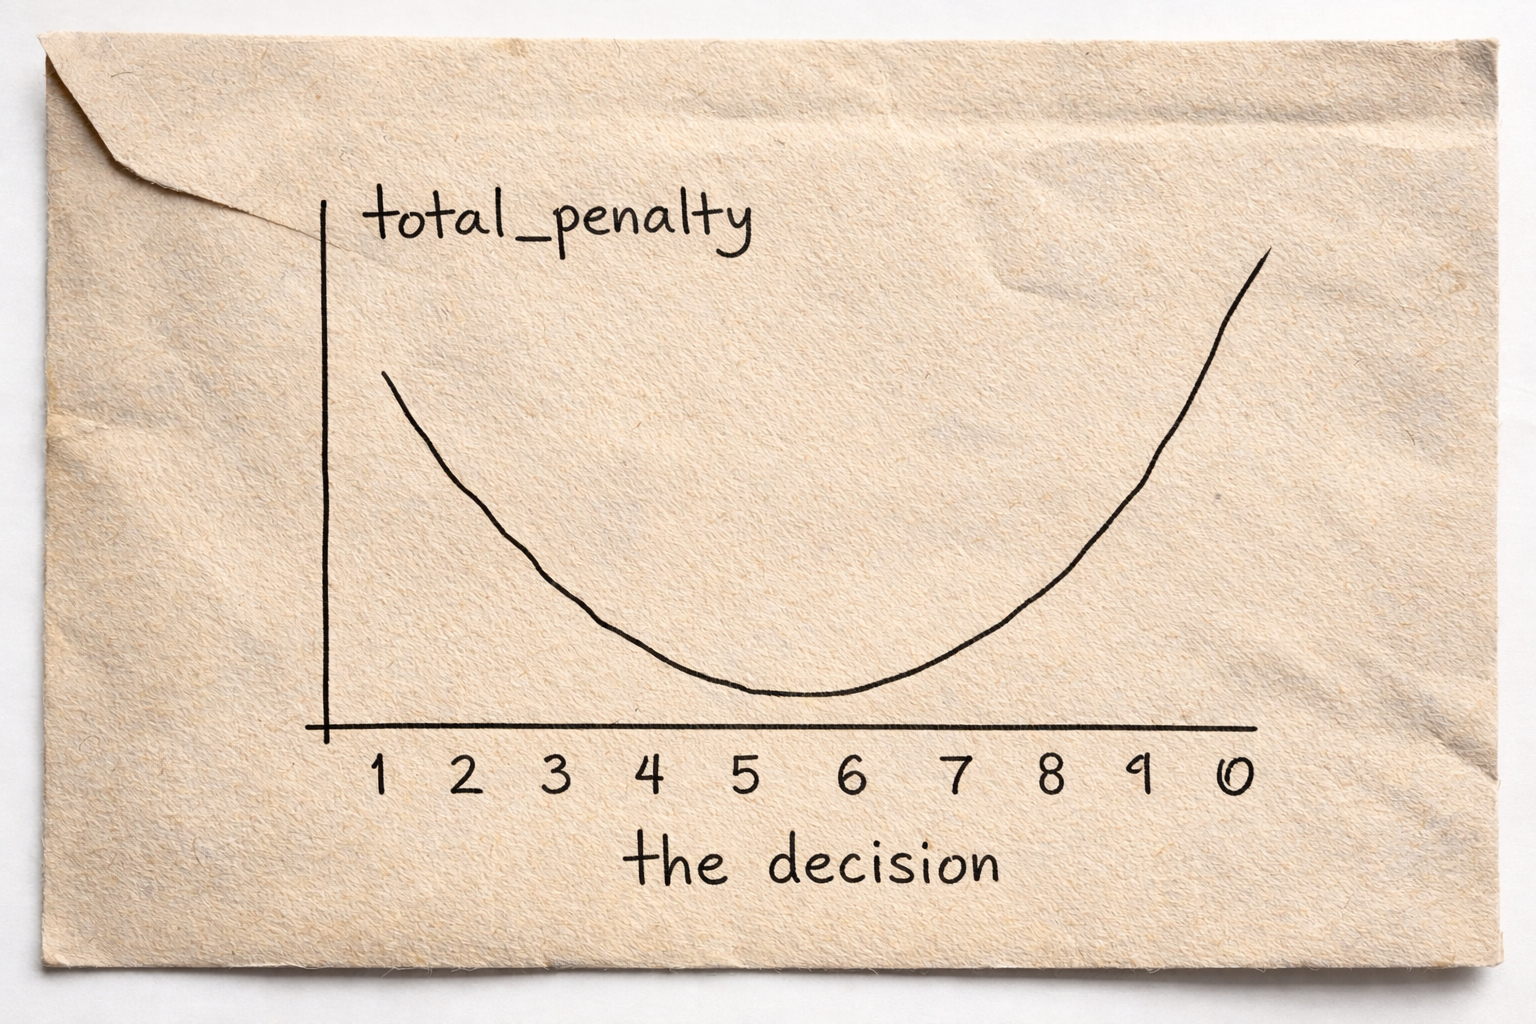
\includegraphics[width=0.7\linewidth,height=\textheight,keepaspectratio]{modules/03-introduction-to-models/../../images/fig-igor-sketch.png}

}

\caption{\label{fig-igor-sketch}Igor's back of the envelope sketch of
the plot that he thought would help them identify the best decision}

\end{figure}%

``If we can generate this plot, we might be able to sell the idea to
Amanda'' Steve said.

\begin{tcolorbox}[enhanced jigsaw, colback=white, leftrule=.75mm, toprule=.15mm, bottomtitle=1mm, breakable, coltitle=black, toptitle=1mm, title={Quick Check}, opacitybacktitle=0.6, colbacktitle=quarto-callout-note-color!10!white, arc=.35mm, left=2mm, colframe=quarto-callout-note-color-frame, titlerule=0mm, rightrule=.15mm, bottomrule=.15mm, opacityback=0]

How do you think Igor's sketch in Figure~\ref{fig-igor-sketch} might be
useful in finding the best decision?

\end{tcolorbox}

\begin{tcolorbox}[enhanced jigsaw, colback=white, leftrule=.75mm, toprule=.15mm, bottomtitle=1mm, breakable, coltitle=black, toptitle=1mm, title={Suggested answer}, opacitybacktitle=0.6, colbacktitle=quarto-callout-note-color!10!white, arc=.35mm, left=2mm, colframe=quarto-callout-note-color-frame, titlerule=0mm, rightrule=.15mm, bottomrule=.15mm, opacityback=0]

If the plot does in fact come out to have this shape, then the decision
where the total penalty is lowest would be good. The plot once actually
generated can help us to find the best decision.

\end{tcolorbox}

``But Igor, this is easier said than done. How can we complete all these
computations in an hour? In fact we might not finish in a week!''
bemoaned Angela. Igor agreed. Perhaps he was being too much in the
clouds.

Suzie joined the fray. ``Angela, If what I am thinking of is correct,
this might not be as hard as it seems. I learned R in a class. I think I
can do this in R quickly and get a nice plot that Igor is talking about.
We can have something ready for Amanda by the time she comes back from
her meeting.''

Everyone exulted ``You can do that? Wow!'' and Suzie and Igor got to
work.

They defined the problem clearly to an AI chatbot and asked it to
generate a program in the R language that could generate the plot. They
described precisely what they wanted the program to do. This part took
some time as they wanted to be very sure that the chatbot had the right
information.

Once they were done, the chatbot then gave them the code in less than a
minute. She looked over it carefully, fixed a few things and then ran
it.

Soon Suzie had a nice plot of the total errors for every possible value
of the decision from 1 through 9 in intervals of 0.2. In fact she had
made 10,000 trials for each value instead of just 1,000 as Igor had
suggested. It looks like a guess of 4 would produce the smallest total
penalty. The team had its answer for Amanda!
Figure~\ref{fig-amanda-simulation} shows the plot. The plot shows that a
decision of 4 generates the lowest total penalty.

\begin{figure}

\centering{

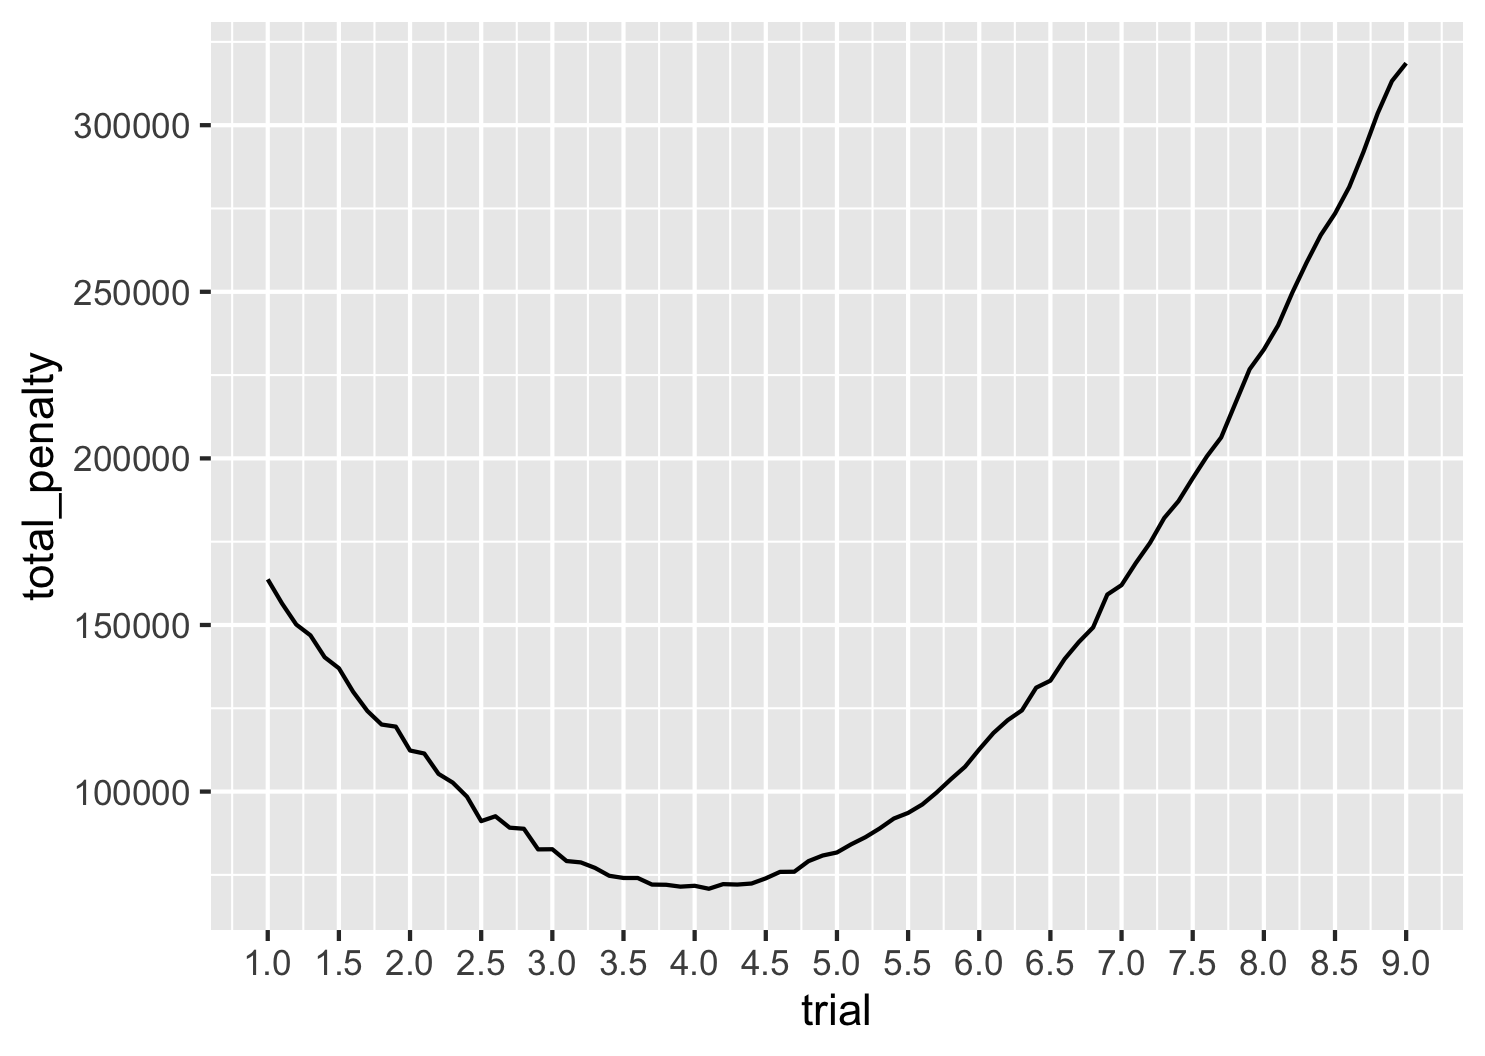
\includegraphics[width=0.7\linewidth,height=\textheight,keepaspectratio]{modules/03-introduction-to-models/../../images/fig-amanda-simulation.png}

}

\caption{\label{fig-amanda-simulation}Results of Suzie's program showing
the various possible decisions and their total penalties: the lowest
total penalty occurs at a decision of 4}

\end{figure}%

High-fives all round.

\begin{tcolorbox}[enhanced jigsaw, colback=white, leftrule=.75mm, toprule=.15mm, bottomtitle=1mm, breakable, coltitle=black, toptitle=1mm, title={Quick Check}, opacitybacktitle=0.6, colbacktitle=quarto-callout-note-color!10!white, arc=.35mm, left=2mm, colframe=quarto-callout-note-color-frame, titlerule=0mm, rightrule=.15mm, bottomrule=.15mm, opacityback=0]

How many values of decision did Suzie's program try out?

\end{tcolorbox}

\begin{tcolorbox}[enhanced jigsaw, colback=white, leftrule=.75mm, toprule=.15mm, bottomtitle=1mm, breakable, coltitle=black, toptitle=1mm, title={Suggested answer}, opacitybacktitle=0.6, colbacktitle=quarto-callout-note-color!10!white, arc=.35mm, left=2mm, colframe=quarto-callout-note-color-frame, titlerule=0mm, rightrule=.15mm, bottomrule=.15mm, opacityback=0]

She tried the values 1, 1.2, 1.4, 1.6, 1.8, or 5 values between 1 and 2.
Similarly 5 between 2 and 3 and so on That would be 8 times 5 or 40 up
to 8.75. and then there is 9. So she tried a total of 41 different
decision values.

\end{tcolorbox}

\begin{tcolorbox}[enhanced jigsaw, colback=white, leftrule=.75mm, toprule=.15mm, bottomtitle=1mm, breakable, coltitle=black, toptitle=1mm, title={Quick Check}, opacitybacktitle=0.6, colbacktitle=quarto-callout-note-color!10!white, arc=.35mm, left=2mm, colframe=quarto-callout-note-color-frame, titlerule=0mm, rightrule=.15mm, bottomrule=.15mm, opacityback=0]

How many individual differences did her program compute?

\end{tcolorbox}

\begin{tcolorbox}[enhanced jigsaw, colback=white, leftrule=.75mm, toprule=.15mm, bottomtitle=1mm, breakable, coltitle=black, toptitle=1mm, title={Suggested answer}, opacitybacktitle=0.6, colbacktitle=quarto-callout-note-color!10!white, arc=.35mm, left=2mm, colframe=quarto-callout-note-color-frame, titlerule=0mm, rightrule=.15mm, bottomrule=.15mm, opacityback=0]

For each decision her program tried 10,000 trials and hence computed
10,000 differences for a total of 10,000*41, or 410,000 differences.

\end{tcolorbox}

``Wait a minute'' said Angela. With Amanda's trials, the total penalty
was close to 200. Now it looks like our lowest is close to 70,000. What
is going on? Have me done something wrong here? I have heard that AI
chatbots can hallucinate. Have wee been hit with a major
hallucination?''

Doom spread in the room. Amanda would be in the room shortly. Have they
let her down badly?

Silent Igor came to their rescue again. ``The total penalty in Amanda's
case was computed over 20 trials. Suzie's total penalties are based on
10,000 trials. Naturally they will be higher. This is an apples to
oranges comparison.

To make these comparable, we should be comparing the average penalty
\textbf{per trial} to remove the direct effect of the number of trials
on the total penalty. So we should divide Amanda's total penalty by 20
and Suzie's by 10,000 to get the average penalty per trial for each of
them. Then we can compare them.''

David immediately did some mental math and came back with ``Well, for
the numbers we tried with Amanda, the average penalty per trial was
approximately 220/20, or 11. For Suzie's numbers, the plot says that the
total penalty for the best decision of 4 is around 70,000. We divide
that by 10,000 trials and get a penalty per trial of 7. So we did
improve significantly on what we initially came up with.''

The group heaved collective sign of relief.

Igor said ``Since Suzie did 10,000 trials for each number, we can be
almost certain that 4 is in fact \emph{the best solution}.

The team had finished with 10 minutes to spare. They spent the remaining
time preparing a neat presentation for Amanda describing exactly what
they had done. They also explained how they had used AI to help in this
process.

When she returned, Amanda took one look at the chart and asked a few
questions about how they had generated it. She was convinced that these
young interns had found the best solution to her kisok staffing problem.

Amanda said ``Thank you all very much. You have done a great job! You
accomplished a lot in a short amount of time. Do you know why that
happened?

You worked as a team. Your ideas built upon each other and you were able
to achieve a lot.

How do I know even though I was not in the room? Well, I have seen this
time and again, and you will too in your working lives. That's the
strength of teams -- some say Wisdom of Teams.

We will meet next month to review how things went and to refine our
decisions.''

\section{\texorpdfstring{Average or \emph{mean} as the decision in the
long
run}{Average or mean as the decision in the long run}}\label{average-or-mean-as-the-decision-in-the-long-run}

David had a thought. ``Let us try the decision value of 4 using Amanda's
approach and see what total penalty we get for 20 trials.''

They did, and Table~\ref{tbl-decision-penalty-4} shows that indeed the
total penalty for this is lower than the first two and the average
penalty per trial is 166/20. This is higher than the average of 7 with
10,000 trials, but we can chalk it up to using only 20 trials.

\begin{longtable}[]{@{}rrr@{}}
\caption{Decision, random choices, and resulting penalties (Decision =
4)}\label{tbl-decision-penalty-4}\tabularnewline
\toprule\noalign{}
\multicolumn{2}{@{}r}{%
Decision =} & 4 \\
random\_choice & diff & penalty \\
\midrule\noalign{}
\endfirsthead
\toprule\noalign{}
\multicolumn{2}{@{}r}{%
Decision =} & 4 \\
random\_choice & diff & penalty \\
\midrule\noalign{}
\endhead
\bottomrule\noalign{}
\endlastfoot
8 & -4 & 16 \\
2 & 2 & 4 \\
1 & 3 & 9 \\
2 & 2 & 4 \\
4 & 0 & 0 \\
4 & 0 & 0 \\
8 & -4 & 16 \\
2 & 2 & 4 \\
8 & -4 & 16 \\
8 & -4 & 16 \\
4 & 0 & 0 \\
4 & 0 & 0 \\
9 & -5 & 25 \\
1 & 3 & 9 \\
3 & 1 & 1 \\
9 & -5 & 25 \\
2 & 2 & 4 \\
2 & 2 & 4 \\
1 & 3 & 9 \\
2 & 2 & 4 \\
\multicolumn{2}{@{}r}{%
Total penalty =} & 166 \\
\end{longtable}

So what is special about 4? Given another set of numbers, do we have to
repeat this charting process that Suzie did for each set of numbers?

Well, 4 happens to be the average of the numbers. It turns out that when
we have a large number of trials, we will get the best results, that is
the lowest total penalty, when we always guess the average of the
numbers. In this case the average is 4.

So, we see that in the absence of any other information to help us
predict, the best prediction is the \emph{mean}.
Figure~\ref{fig-many-nos-one-pred} shows this pictorially.

\begin{figure}

\centering{


\includegraphics[width=0.7\linewidth,height=\textheight,keepaspectratio]{modules/03-introduction-to-models/../../images/fig-many-nos-one-pred.png}

}

\caption{\label{fig-many-nos-one-pred}Many numbers, but just a single
prediction!}

\end{figure}%

What we have said above \textbf{does not mean that we are guaranteed to
get the smallest total error if we commit to the average}. Clearly, if
someone were lucky enough that the random picks all ended up exactly
equal to or very close to their decision just by chance, then their
total error will be zero! But this is \emph{extremely unlikely}.

However, those occurrences are extraordinarily unlikely with a large
number of trials, as happens in business where a decision is tested by
thousands of events. \emph{Statistically} the best course would be to
pick the average.

\begin{tcolorbox}[enhanced jigsaw, colback=white, leftrule=.75mm, toprule=.15mm, bottomtitle=1mm, breakable, coltitle=black, toptitle=1mm, title={Quick Check}, opacitybacktitle=0.6, colbacktitle=quarto-callout-note-color!10!white, arc=.35mm, left=2mm, colframe=quarto-callout-note-color-frame, titlerule=0mm, rightrule=.15mm, bottomrule=.15mm, opacityback=0]

In what sense is the mean the ``best'' model?

\end{tcolorbox}

\begin{tcolorbox}[enhanced jigsaw, colback=white, leftrule=.75mm, toprule=.15mm, bottomtitle=1mm, breakable, coltitle=black, toptitle=1mm, title={Suggested answer}, opacitybacktitle=0.6, colbacktitle=quarto-callout-note-color!10!white, arc=.35mm, left=2mm, colframe=quarto-callout-note-color-frame, titlerule=0mm, rightrule=.15mm, bottomrule=.15mm, opacityback=0]

``Best'' means minimizing overall prediction error, not being perfect.

\end{tcolorbox}

\begin{tcolorbox}[enhanced jigsaw, colback=white, leftrule=.75mm, toprule=.15mm, bottomtitle=1mm, breakable, coltitle=black, toptitle=1mm, title={Quick Check}, opacitybacktitle=0.6, colbacktitle=quarto-callout-note-color!10!white, arc=.35mm, left=2mm, colframe=quarto-callout-note-color-frame, titlerule=0mm, rightrule=.15mm, bottomrule=.15mm, opacityback=0]

Can a model be ``best'' and still be inaccurate?

\end{tcolorbox}

\begin{tcolorbox}[enhanced jigsaw, colback=white, leftrule=.75mm, toprule=.15mm, bottomtitle=1mm, breakable, coltitle=black, toptitle=1mm, title={Suggested answer}, opacitybacktitle=0.6, colbacktitle=quarto-callout-note-color!10!white, arc=.35mm, left=2mm, colframe=quarto-callout-note-color-frame, titlerule=0mm, rightrule=.15mm, bottomrule=.15mm, opacityback=0]

Yes. A model can be the best available option given limited information
and still perform poorly in absolute terms.

\end{tcolorbox}

\begin{tcolorbox}[enhanced jigsaw, colback=white, leftrule=.75mm, toprule=.15mm, bottomtitle=1mm, breakable, coltitle=black, toptitle=1mm, title={Quick Check}, opacitybacktitle=0.6, colbacktitle=quarto-callout-note-color!10!white, arc=.35mm, left=2mm, colframe=quarto-callout-note-color-frame, titlerule=0mm, rightrule=.15mm, bottomrule=.15mm, opacityback=0]

Does it make intuitive sense that the average turns out to be the best
model? Explain why or why not.

\end{tcolorbox}

\begin{tcolorbox}[enhanced jigsaw, colback=white, leftrule=.75mm, toprule=.15mm, bottomtitle=1mm, breakable, coltitle=black, toptitle=1mm, title={Suggested answer}, opacitybacktitle=0.6, colbacktitle=quarto-callout-note-color!10!white, arc=.35mm, left=2mm, colframe=quarto-callout-note-color-frame, titlerule=0mm, rightrule=.15mm, bottomrule=.15mm, opacityback=0]

It makes sense to guess a number sort of in the middle so that we are
generally close to all numbers that could turn up on random choices. See
s@ec-simple-model-enrichment-1 if you want to thin k about this more.

\end{tcolorbox}

\begin{tcolorbox}[enhanced jigsaw, colback=white, leftrule=.75mm, toprule=.15mm, bottomtitle=1mm, breakable, coltitle=black, toptitle=1mm, title=\textcolor{quarto-callout-important-color}{\faExclamation}\hspace{0.5em}{Interpret the word ``best model'' with caution}, opacitybacktitle=0.6, colbacktitle=quarto-callout-important-color!10!white, arc=.35mm, left=2mm, colframe=quarto-callout-important-color-frame, titlerule=0mm, rightrule=.15mm, bottomrule=.15mm, opacityback=0]

When we say the mean is the best model, we do not mean it is always
accurate, fair, or appropriate. We mean it is best according to a
specific criterion, under specific information constraints.

\end{tcolorbox}

Now you know why I titled the chapter \emph{The simplest Model}!

\section{Real world connection: Planning for Customer
Demand}\label{real-world-connection-planning-for-customer-demand}

How does this small ``practice game'' relate to the real world? Let us
return to the manager's kiosk problem.

A company operates two small sales kiosks in the same city---one at the
\emph{Beach} and one at the \emph{Mall}. The company must decide how
many workers to schedule each day.

\subsection{What the company must do}\label{what-the-company-must-do}

\begin{itemize}
\tightlist
\item
  The staffing decision must be made \textbf{in advance}
\item
  Once the schedule is set, it cannot be easily changed without
  disrupting employees
\item
  In this first round, the manager insists on \textbf{one number} to use
  everywhere (the same staffing plan for both kiosks)
\end{itemize}

\subsection{What the company knows}\label{what-the-company-knows}

\begin{itemize}
\tightlist
\item
  The company has historical data on daily customer counts---but in an
  unhelpful format
\item
  The counts are \textbf{not labeled by kiosk} (Beach vs Mall)
\item
  At this point, the company does not have any data to explain
  \emph{why} customer traffic changes. It simply observes that demand
  varies
\end{itemize}

Here are the 20 historical customer counts (mixed together, with no
kiosk identification):

\begin{lstlisting}
89, 95, 131, 101, 103, 134, 109, 75, 86, 91, 177, 151, 152, 143, 123, 194, 155, 81, 161, 126
\end{lstlisting}

\subsection{Why the decision matters}\label{why-the-decision-matters}

\begin{itemize}
\item
  If too few workers are scheduled:

  \begin{itemize}
  \tightlist
  \item
    customers wait longer
  \item
    service quality suffers
  \item
    some customers leave without buying
  \end{itemize}
\item
  If too many workers are scheduled:

  \begin{itemize}
  \tightlist
  \item
    workers are idle
  \item
    labor cost rises
  \item
    managers waste attention adjusting schedules
  \end{itemize}
\end{itemize}

\subsection{How the company measures
mistakes}\label{how-the-company-measures-mistakes}

\begin{itemize}
\item
  Being slightly wrong is not very costly
\item
  Being very wrong is much more costly
\item
  The manager therefore measures the cost of a decision as:

  \begin{itemize}
  \tightlist
  \item
    the \textbf{square of the difference} between planned customers and
    actual customers
  \end{itemize}
\end{itemize}

\subsection{How the decision is
evaluated}\label{how-the-decision-is-evaluated}

\begin{itemize}
\tightlist
\item
  The decision is \textbf{not judged by a single day}
\item
  A decision that works well once may simply be lucky
\item
  Instead, the manager looks at performance \textbf{across many days}
\item
  Daily customer counts vary, but the staffing decision stays the same
\end{itemize}

\subsection{The conclusion}\label{the-conclusion}

\begin{itemize}
\tightlist
\item
  The manager must choose a single number to plan for
\item
  Under a squared-penalty rule, the number that minimizes total long-run
  cost is the \textbf{average} of past customer counts (here, about
  \textbf{123.8})
\item
  Choosing a smaller number leads to frequent large shortages
\item
  Choosing a larger number leads to frequent over-staffing
\item
  The average balances these errors over time
\end{itemize}

\subsection{Why this matters}\label{why-this-matters}

\begin{itemize}
\tightlist
\item
  This is the first ``model'' you learn in this book: a model that
  predicts the same value every time
\item
  It is simple, but it is not arbitrary---it is the \textbf{best} choice
  given the information available
\item
  Later chapters improve on this model by adding explanatory information
  (first categories, then numerical predictors)
\end{itemize}

\section{Optional enrichment topic: How does skew affect the
situation?}\label{optional-enrichment-topic-how-does-skew-affect-the-situation}

In our practice game, we used the numbers:

\begin{lstlisting}
4, 2, 6, 1, 8, 1, 3, 9, 2, 4
\end{lstlisting}

in our game. That set has numbers across the entire range. Is it the
case that the average performed well because of this? Could it be that
the average will not perform well if most of the numbers fall within in
a small range and a few extreme cases tend to push the average up?

For, example, let us take the following set of numbers:

\begin{lstlisting}
2, 1, 2, 1, 3, 3, 2, 1, 10, 9
\end{lstlisting}

The mean is 3.4. However, this set has eight of its numbers less than or
equal to 3. Perhaps a decision below the average will work better?

Let us play the game 10,000 times and see which decision performs best.

Figure~\ref{fig-simulation-game-summary-skewed} shows the results. We
see that the mean is still the best \emph{decision}.

\begin{figure}

\centering{

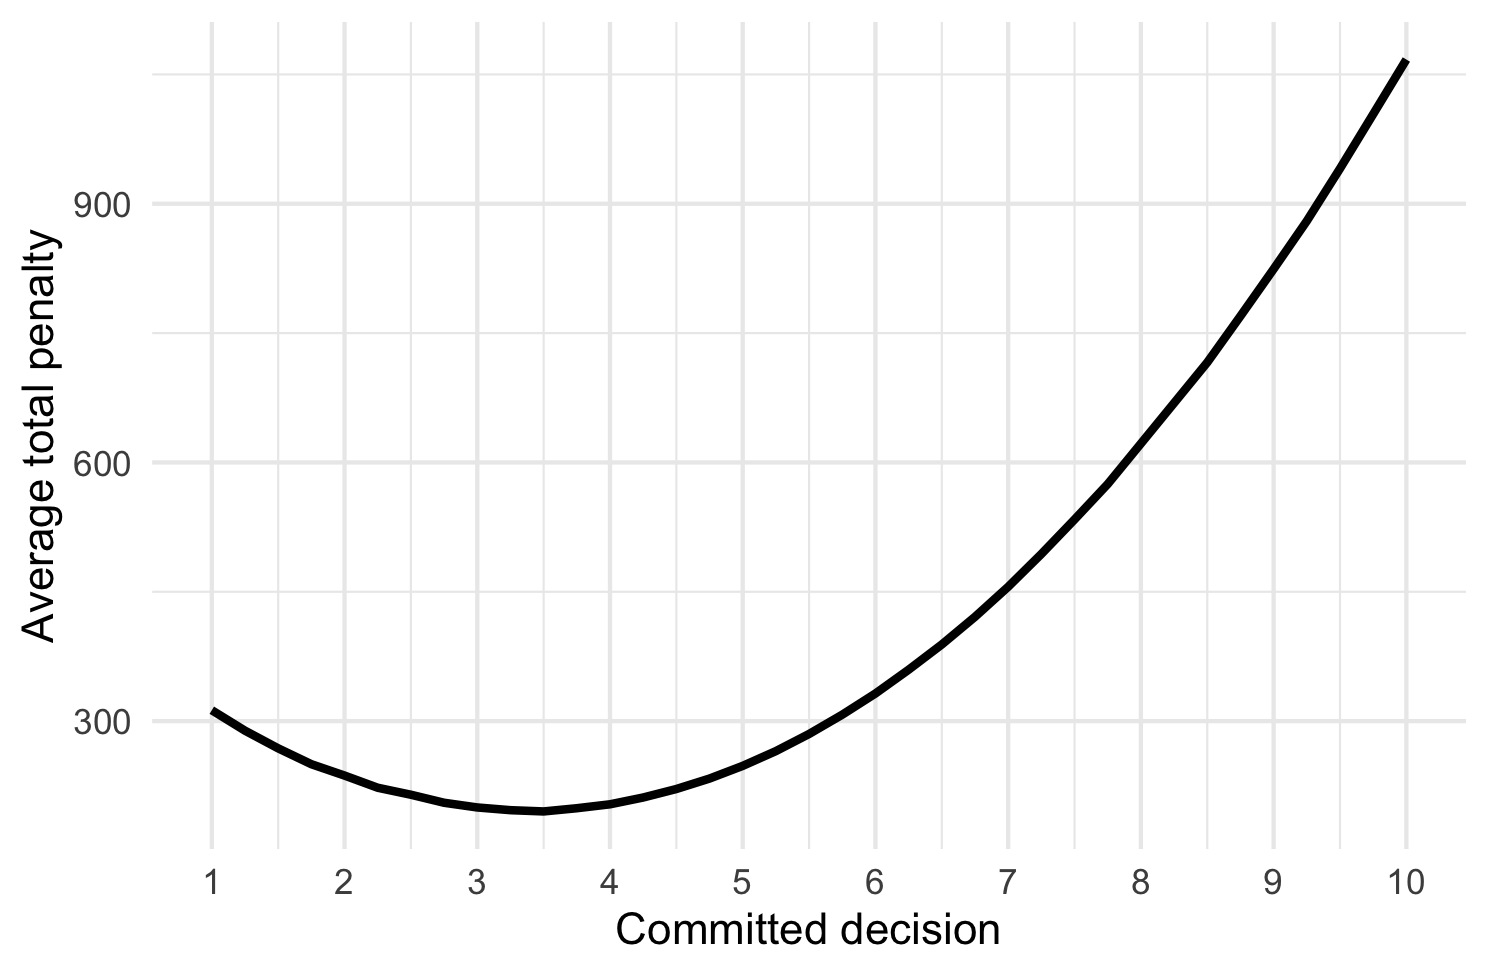
\includegraphics[width=0.7\linewidth,height=\textheight,keepaspectratio]{modules/03-introduction-to-models/../../images/fig-simulation-game-summary-skewed.png}

}

\caption{\label{fig-simulation-game-summary-skewed}Average of
\emph{total\_penalty} vs various values for \emph{decision} based on
10,000 plays of the game -- shows that the lowest total penalty overall
occurs when \emph{decision} equals the mean of the numbers}

\end{figure}%

Why does this happen? Choosing the average definitely leads to small
penalty increases most of the time. However, if we went below the
average, the relatively rare cases in which the random choice is high,
it incurs a very large penalty and that offsets any benefits of going
below the average, because we square the difference and that amplifies
the error.

\textbf{What if we did not square the error and instead treated the
absolute difference as the penalty. In this case, the \emph{median} is
the best choice.} Pretty cool result if you as me! We will not go
further into that topic, but it has its applications. In most practical
applications, we use the squared-difference as the penalty.

\begin{tcolorbox}[enhanced jigsaw, colback=white, leftrule=.75mm, toprule=.15mm, bottomtitle=1mm, breakable, coltitle=black, toptitle=1mm, title={Pause \& Think}, opacitybacktitle=0.6, colbacktitle=quarto-callout-note-color!10!white, arc=.35mm, left=2mm, colframe=quarto-callout-note-color-frame, titlerule=0mm, rightrule=.15mm, bottomrule=.15mm, opacityback=0]

\begin{enumerate}
\def\labelenumi{\arabic{enumi}.}
\tightlist
\item
  If two data sets have the same mean, could the mean be a better model
  for one than the other?
\item
  What additional information might help you judge if it will work
  better for one than for the other?
\end{enumerate}

\end{tcolorbox}

\begin{tcolorbox}[enhanced jigsaw, colback=white, leftrule=.75mm, toprule=.15mm, bottomtitle=1mm, breakable, coltitle=black, toptitle=1mm, title={Suggested answers}, opacitybacktitle=0.6, colbacktitle=quarto-callout-note-color!10!white, arc=.35mm, left=2mm, colframe=quarto-callout-note-color-frame, titlerule=0mm, rightrule=.15mm, bottomrule=.15mm, opacityback=0]

\begin{enumerate}
\def\labelenumi{\arabic{enumi}.}
\tightlist
\item
  Yes. The mean works better when observations are tightly clustered.
\item
  Variability, spread, or deviation from the mean would help evaluate
  model quality.
\end{enumerate}

\end{tcolorbox}

\section{Optional enrichment topic: Removing outliers in skewed
distributions}\label{sec-simple-model-enrichment-1}

Continuing from the prior discussion, when faced with a skewed
distribution we have a peculiar situation where our intuition tells us
to make a decision where most points lie, but cold computation tells us
otherwise.

One may feel that it makes no sense to choose the mean and accumulate a
slightly higher penalty in every event just to balance out the huge
penalties that come rarely. But that is what makes sense when we use the
quadratic penalty function.

If the penalty is quadratic, but we still want to not decide on the
average, then we can eliminate the extreme points and reduce the skew.
Then we can use the average as before. From a practical viewpoint what
that would mean is that we take steps to avoid extreme events by some
means.

Interestingly, if we do not square the differences and simply add the
absolute values of the differences to compute the total penalty, then
the median (or the middle value among the numbers when they are ordered
by magnitude) is the best decision. I find that result very cool!

Can you think of an experiment to compare removing outliers and not
removing them in the context of skewed distributions to see if using the
mean in both cases reduces the total penalty significantly?

You can delve deeper into this topic if you are interested.

\chapter{Category Means}\label{sec-category-means}

Angela, Steve, Dave, Igor, and Suzie -- our interns from the previous
chapter, sat around the table in the conference room waiting for Amanda
and discussed the previous night's exciting professional basketball
game.

Last chapter, the interns learned an important lesson: when you must
commit to \textbf{one number} without any further information, and you
measure mistakes more harshly the bigger they are (by using a squared
penalty), the best long-run choice is the average.

\begin{tcolorbox}[enhanced jigsaw, colback=white, leftrule=.75mm, toprule=.15mm, bottomtitle=1mm, breakable, coltitle=black, toptitle=1mm, title={Quick Check}, opacitybacktitle=0.6, colbacktitle=quarto-callout-note-color!10!white, arc=.35mm, left=2mm, colframe=quarto-callout-note-color-frame, titlerule=0mm, rightrule=.15mm, bottomrule=.15mm, opacityback=0]

Why was the average the best choice \emph{in the previous chapter},
given the information available at that time?

\end{tcolorbox}

\begin{tcolorbox}[enhanced jigsaw, colback=white, leftrule=.75mm, toprule=.15mm, bottomtitle=1mm, breakable, coltitle=black, toptitle=1mm, title={Suggested answer}, opacitybacktitle=0.6, colbacktitle=quarto-callout-note-color!10!white, arc=.35mm, left=2mm, colframe=quarto-callout-note-color-frame, titlerule=0mm, rightrule=.15mm, bottomrule=.15mm, opacityback=0]

Because the company had to commit to a single number for all situations
and used a squared penalty for mistakes, the average minimized the
long-run penalty. With no additional information to distinguish cases,
no other single number could do better on average.

\end{tcolorbox}

Amanda walked in exactly at 9 am. WIth a bright smile, she said ``Team,
I have some good news. First off, we did very well last month. We had
far fewer days of bad mismatches from our staffing levels with the
customer counts. Your model improved significantly on what we were doing
earlier.

Secondly, I have better data this time and I am hoping we can improve
our decision further.''

\section{Staffing kiosks at malls and
beaches}\label{staffing-kiosks-at-malls-and-beaches}

``I have better data this time'' Amanda says, pulling up a spreadsheet
on her laptop. ``The same two kiosks. Same city. Same staffing problem.
But \ldots{}''

She points to the new column.

``This time, the person collecting data included the kiosk.''

The interns lean in. The data now tells them \emph{where} each customer
count came from: \emph{Mall} or \emph{Beach}.

\begin{tcolorbox}[enhanced jigsaw, colback=white, leftrule=.75mm, toprule=.15mm, bottomtitle=1mm, breakable, coltitle=black, toptitle=1mm, title={Quick Check}, opacitybacktitle=0.6, colbacktitle=quarto-callout-note-color!10!white, arc=.35mm, left=2mm, colframe=quarto-callout-note-color-frame, titlerule=0mm, rightrule=.15mm, bottomrule=.15mm, opacityback=0]

What new kind of decision does the presence of the \emph{kiosk} column
make possible?

\end{tcolorbox}

\begin{tcolorbox}[enhanced jigsaw, colback=white, leftrule=.75mm, toprule=.15mm, bottomtitle=1mm, breakable, coltitle=black, toptitle=1mm, title={Suggested answer}, opacitybacktitle=0.6, colbacktitle=quarto-callout-note-color!10!white, arc=.35mm, left=2mm, colframe=quarto-callout-note-color-frame, titlerule=0mm, rightrule=.15mm, bottomrule=.15mm, opacityback=0]

It allows the company to make different decisions for different
situations. Instead of committing to one number for all days for both
kiosks, the company can now choose separate staffing levels for the Mall
kiosk and for the Beach kiosk.

\end{tcolorbox}

The key difference from the previous chapter is that the decision no
longer has to be the same everywhere. Instead, the company can make one
decision for the Mall kiosk and a different decision for the Beach
kiosk, using the information it has about location. Amanda hoped that
this can lead to an even better match between the staffing and the
actual customer numbers.

Here is the data:

\begin{longtable}[]{@{}rl@{}}
\toprule\noalign{}
customers & kiosk \\
\midrule\noalign{}
\endhead
\bottomrule\noalign{}
\endlastfoot
89 & Mall \\
95 & Mall \\
131 & Mall \\
101 & Mall \\
103 & Mall \\
134 & Mall \\
109 & Mall \\
75 & Mall \\
86 & Mall \\
91 & Mall \\
177 & Beach \\
151 & Beach \\
152 & Beach \\
143 & Beach \\
123 & Beach \\
194 & Beach \\
155 & Beach \\
81 & Beach \\
161 & Beach \\
126 & Beach \\
\end{longtable}

Amanda taps the screen.

``Last month I asked for, and you gave me, \emph{one} figure for the
number of customers for both kiosks'' she says. ``Now we have more
information and want to do better. Can you use this extra information?''

In this scenario, we need to decide a customer level to use for
determining staff level -- but separately for each kiosk.

\begin{itemize}
\item
  If we are given only the data in column 1 (the \emph{customers}
  counts), then based on the previous chapter, our best choice is the
  overall average.
\item
  If we are given the entire table, then we have additional information
  and can possibly determine a different number for each kiosk.
\end{itemize}

Initially it seems to many of the interns that the new information
really does not add any value. David says, ``Why not just adopt the
overall average again like last month? I mean how is this kiosk
information helping us?''

Angela says ``Let us consider an extreme scenario. What if the sales at
the Beach kiosk is generally twice that of the sales in the Mall kiosk.
In that case, predicting the same number for both does not seem right.
Surely we will not have the same staffing level for both. So
differentiating the two should make sense.''

``I agree'' Suzie says. ``We should first look at the data. Even if the
difference in sales is not as dramatic as Angela mentioned, it might
still make sense to differentiate. I have computed the averages for the
two kiosks. Here they are.'' Suzie then shows
Table~\ref{tbl-kiosk-avg-sales}.

\begin{longtable}[]{@{}lr@{}}
\caption{Average sales at the two
kiosks}\label{tbl-kiosk-avg-sales}\tabularnewline
\toprule\noalign{}
kiosk & avg\_customers \\
\midrule\noalign{}
\endfirsthead
\toprule\noalign{}
kiosk & avg\_customers \\
\midrule\noalign{}
\endhead
\bottomrule\noalign{}
\endlastfoot
Mall & 101 \\
Beach & 146 \\
\end{longtable}

David: ``I see your point. These sales do seem quite different with the
beach kiosk getting 40\% more customers per day on average. Perhaps a
different model value does make sense after all. What should the value
be though for each kiosk?''

Again, Igor speaks last, a little less timid than he was the last time
around. ``If we treat the data separately for each kiosk then we really
have two problems that are identical to our problem from last month.''

\begin{tcolorbox}[enhanced jigsaw, colback=white, leftrule=.75mm, toprule=.15mm, bottomtitle=1mm, breakable, coltitle=black, toptitle=1mm, title={Quick Check}, opacitybacktitle=0.6, colbacktitle=quarto-callout-note-color!10!white, arc=.35mm, left=2mm, colframe=quarto-callout-note-color-frame, titlerule=0mm, rightrule=.15mm, bottomrule=.15mm, opacityback=0]

Why does splitting the data by kiosk turn this problem into two familiar
problems from the previous chapter?

\end{tcolorbox}

\begin{tcolorbox}[enhanced jigsaw, colback=white, leftrule=.75mm, toprule=.15mm, bottomtitle=1mm, breakable, coltitle=black, toptitle=1mm, title={Suggested answer}, opacitybacktitle=0.6, colbacktitle=quarto-callout-note-color!10!white, arc=.35mm, left=2mm, colframe=quarto-callout-note-color-frame, titlerule=0mm, rightrule=.15mm, bottomrule=.15mm, opacityback=0]

Once the data are split, each kiosk requires committing to a single
number for it without further distinctions. That is exactly the same
decision problem as before, just applied separately to each kiosk's
data.

\end{tcolorbox}

Peter: ``Then should we just say the model value for each kiosk's is its
own average sales?''

The rest nods in agreement. They cannot see any flaw in this.

Peter: ``For the \emph{Mall} kiosk, we can use the average of the
\emph{customers} column for only the \emph{Mall} rows, and similarly for
the \emph{Beach} kiosk.''

\begin{tcolorbox}[enhanced jigsaw, colback=white, leftrule=.75mm, toprule=.15mm, bottomtitle=1mm, breakable, coltitle=black, toptitle=1mm, title={Quick Check}, opacitybacktitle=0.6, colbacktitle=quarto-callout-note-color!10!white, arc=.35mm, left=2mm, colframe=quarto-callout-note-color-frame, titlerule=0mm, rightrule=.15mm, bottomrule=.15mm, opacityback=0]

Looking at the two kiosk averages in Table~\ref{tbl-kiosk-avg-sales},
what would go wrong if we used the \emph{Mall} average to staff the
\emph{Beach} kiosk?

\end{tcolorbox}

\begin{tcolorbox}[enhanced jigsaw, colback=white, leftrule=.75mm, toprule=.15mm, bottomtitle=1mm, breakable, coltitle=black, toptitle=1mm, title={Suggested answer}, opacitybacktitle=0.6, colbacktitle=quarto-callout-note-color!10!white, arc=.35mm, left=2mm, colframe=quarto-callout-note-color-frame, titlerule=0mm, rightrule=.15mm, bottomrule=.15mm, opacityback=0]

The Beach kiosk typically serves many more customers than the Mall
kiosk. Using the Mall average would systematically under-staff the Beach
kiosk, leading to large penalties on many days.

\end{tcolorbox}

\begin{tcolorbox}[enhanced jigsaw, colback=white, leftrule=.75mm, toprule=.15mm, bottomtitle=1mm, breakable, coltitle=black, toptitle=1mm, title={Quick Check}, opacitybacktitle=0.6, colbacktitle=quarto-callout-note-color!10!white, arc=.35mm, left=2mm, colframe=quarto-callout-note-color-frame, titlerule=0mm, rightrule=.15mm, bottomrule=.15mm, opacityback=0]

If Mall and Beach kiosks truly had similar customer traffic, would using
separate decisions still help? Why or why not?

\end{tcolorbox}

\begin{tcolorbox}[enhanced jigsaw, colback=white, leftrule=.75mm, toprule=.15mm, bottomtitle=1mm, breakable, coltitle=black, toptitle=1mm, title={Suggested answer}, opacitybacktitle=0.6, colbacktitle=quarto-callout-note-color!10!white, arc=.35mm, left=2mm, colframe=quarto-callout-note-color-frame, titlerule=0mm, rightrule=.15mm, bottomrule=.15mm, opacityback=0]

If the two kiosks had similar distributions of customer traffic, then
separating them would not provide much benefit. The advantage of using
different decisions comes only when the additional information
meaningfully distinguishes different situations.

\end{tcolorbox}

Angela: ``Can we verify this with a chart like we did the last time?
Except that we will have one chart per kiosk.''

Suzie: ``Since the computer is going to do all the work, we can also
compare the average penalty per trial for the two kiosks and compare
that with using the overall average.''\,''

Suzie's plots for the average penalty for different guesses for each of
the kiosks appear in Figure~\ref{fig-kiosk-beach-plots}.

\begin{figure}

\centering{

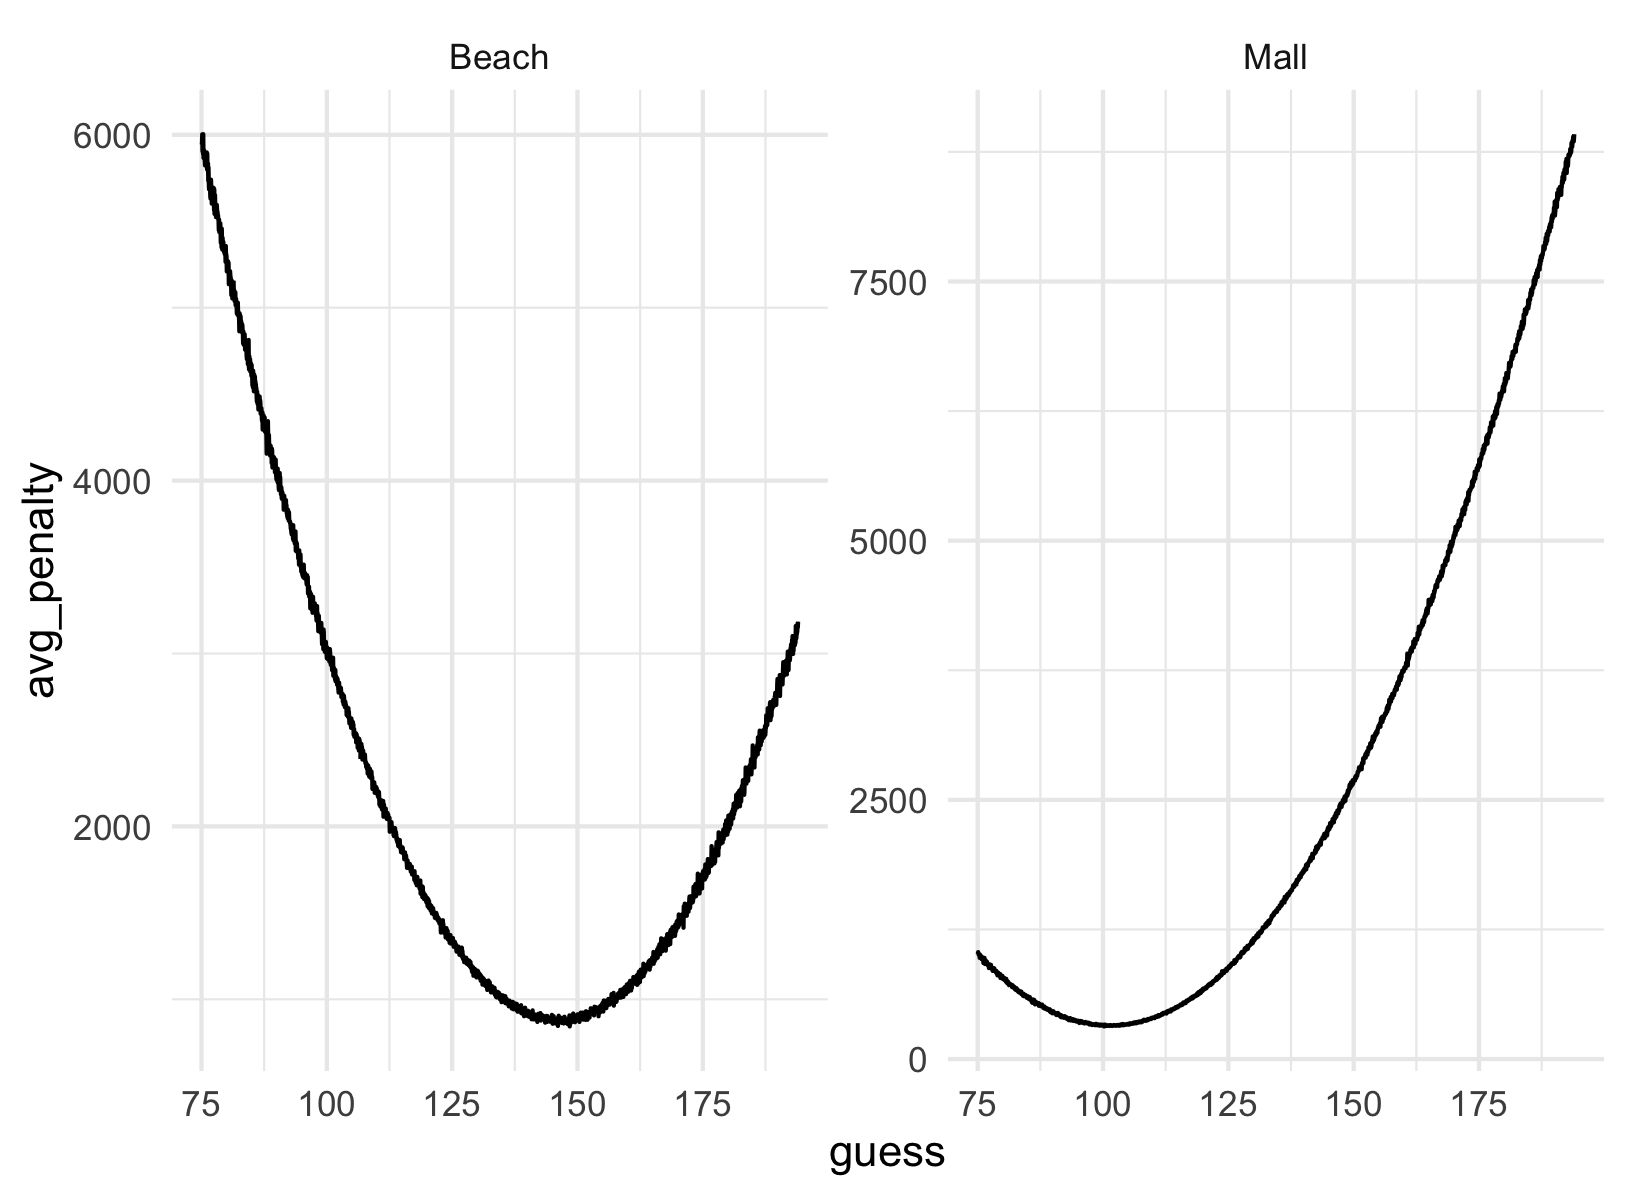
\includegraphics[width=0.7\linewidth,height=\textheight,keepaspectratio]{modules/03-introduction-to-models/../../images/fig-kiosk-beach-plots.png}

}

\caption{\label{fig-kiosk-beach-plots}Plots of guess against average
penalty for the two kiosks: As expected, choosing the average (101 for
mall, and 146 for beach) generates the lowest average penalty}

\end{figure}%

Dave says ``As we expected, the best decisions for the two kiosks is
still the average, but computed separately for each kiosk. In the plot
for the beach kiosk, the lowest average penalty occurs at its average of
146 and at 101 for the mall kiosk.''

Suzie also reported the average penalties if we used the overall average
of number of customers and if we used the specific averages for each
kiosk.

\begin{itemize}
\tightlist
\item
  Average penalty per choice if we use the overall average number of
  customers: 1114
\item
  Average penalty per choice if we use kiosk-specific average for Mall:
  325
\item
  Average penalty per choice if we use kiosk-specific average for Beach:
  880
\end{itemize}

\begin{tcolorbox}[enhanced jigsaw, colback=white, leftrule=.75mm, toprule=.15mm, bottomtitle=1mm, breakable, coltitle=black, toptitle=1mm, title={Quick Check}, opacitybacktitle=0.6, colbacktitle=quarto-callout-note-color!10!white, arc=.35mm, left=2mm, colframe=quarto-callout-note-color-frame, titlerule=0mm, rightrule=.15mm, bottomrule=.15mm, opacityback=0]

Why does using kiosk-specific averages reduce the total penalty compared
to using one overall average?

\end{tcolorbox}

\begin{tcolorbox}[enhanced jigsaw, colback=white, leftrule=.75mm, toprule=.15mm, bottomtitle=1mm, breakable, coltitle=black, toptitle=1mm, title={Suggested answer}, opacitybacktitle=0.6, colbacktitle=quarto-callout-note-color!10!white, arc=.35mm, left=2mm, colframe=quarto-callout-note-color-frame, titlerule=0mm, rightrule=.15mm, bottomrule=.15mm, opacityback=0]

The overall average ignores meaningful differences between kiosks. By
tailoring decisions to each kiosk's typical customer level, the
predictions are closer to actual outcomes for the specific kiosks more
often, reducing squared penalties.

\end{tcolorbox}

We can see that the penalty is far lower if we use the kiosk-specific
averages rather than one overall average. Why is the average penalty so
much higher for the beach kiosk than the mall kiosk? Let us see the
variability in the data for these two kiosks. See
Figure~\ref{fig-kiosk-violin-mall-beach}.

\begin{lstlisting}[language=R]
kiosk_mall_beach |> 
  point_plot(customers ~ kiosk, annot = "violin")
\end{lstlisting}

\begin{figure}

\centering{

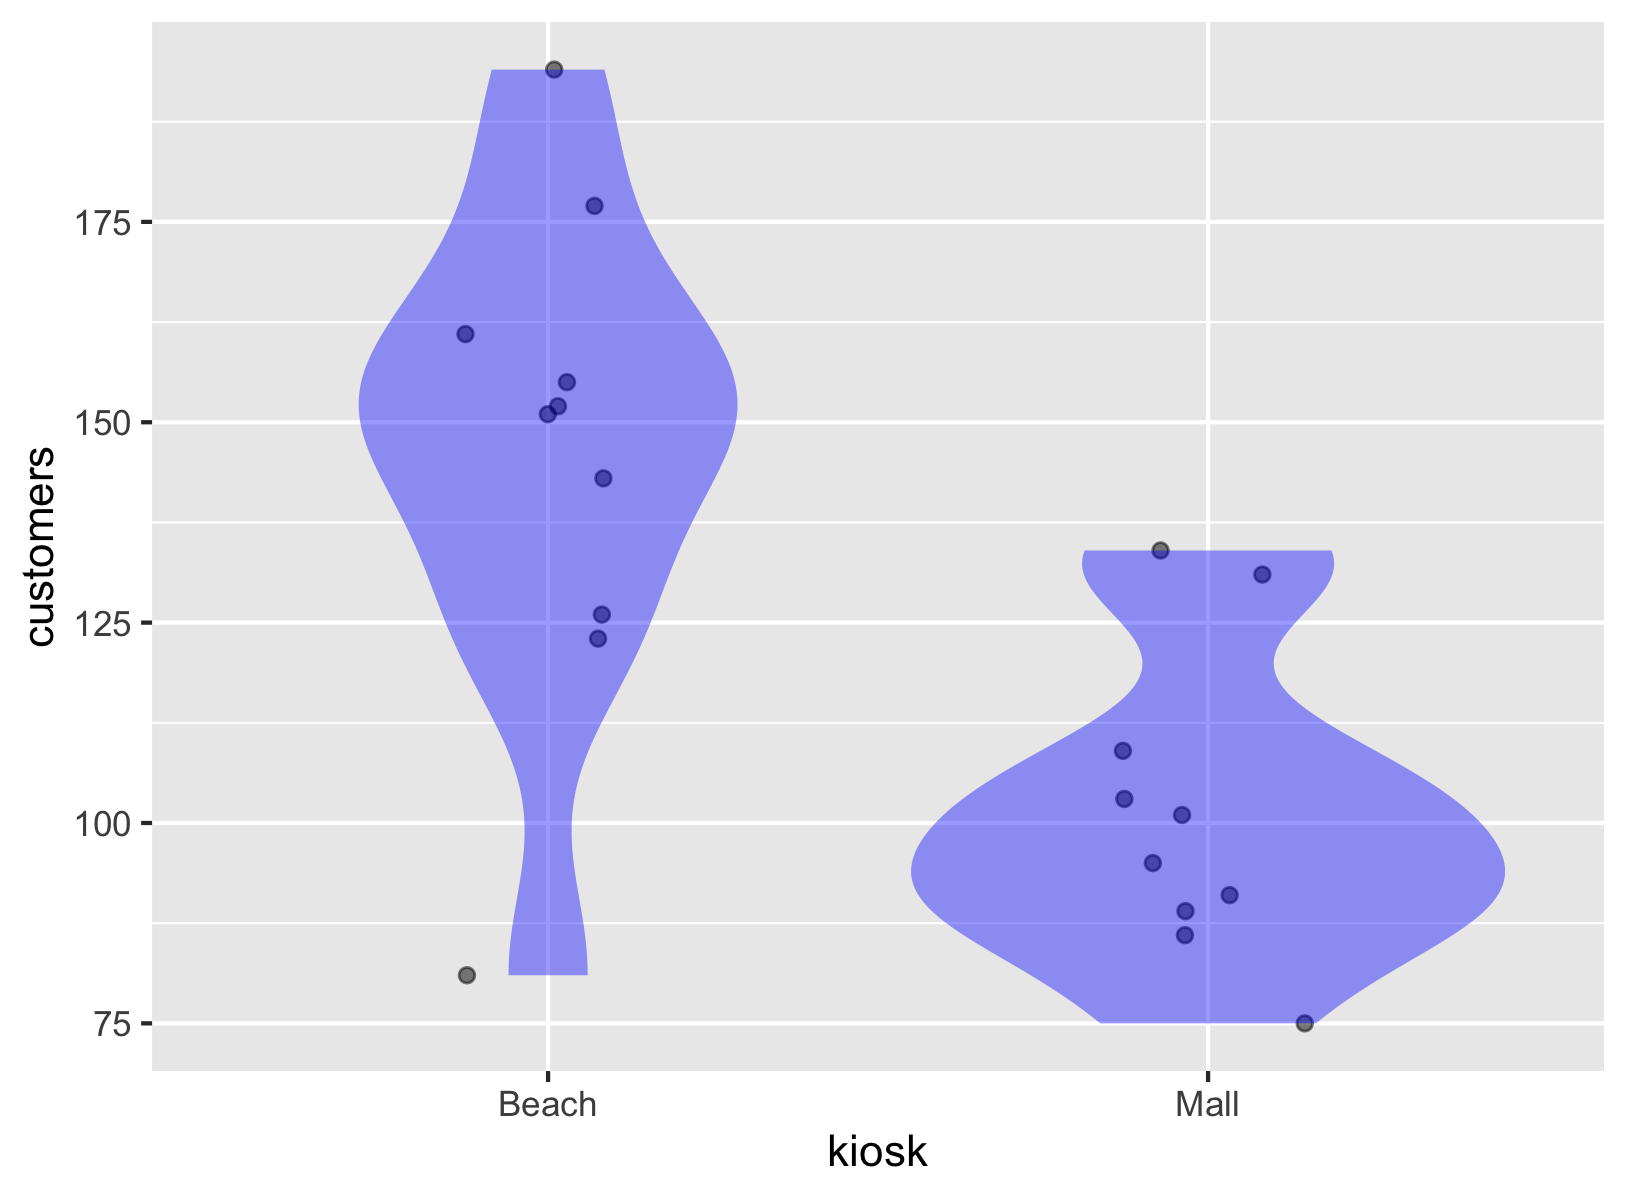
\includegraphics[width=0.7\linewidth,height=\textheight,keepaspectratio]{modules/03-introduction-to-models/../../images/fig-kiosk-violin-mall-beach.png}

}

\caption{\label{fig-kiosk-violin-mall-beach}Comparison of the
distributions of the customer traffic for the two kiosks: Beach has a
lot more variability}

\end{figure}%

Since the beach kiosk has a lot more variability than the mall kiosk,
the penalty is much more, since choosing the average as the decision
will be off from the actual value by quite a bit on many days.

\begin{tcolorbox}[enhanced jigsaw, colback=white, leftrule=.75mm, toprule=.15mm, bottomtitle=1mm, breakable, coltitle=black, toptitle=1mm, title={Quick Check}, opacitybacktitle=0.6, colbacktitle=quarto-callout-note-color!10!white, arc=.35mm, left=2mm, colframe=quarto-callout-note-color-frame, titlerule=0mm, rightrule=.15mm, bottomrule=.15mm, opacityback=0]

Even though the Beach kiosk uses its own average, why is its penalty for
the beach kiosk still higher than the Mall kiosk's?

\end{tcolorbox}

\begin{tcolorbox}[enhanced jigsaw, colback=white, leftrule=.75mm, toprule=.15mm, bottomtitle=1mm, breakable, coltitle=black, toptitle=1mm, title={Suggested answer}, opacitybacktitle=0.6, colbacktitle=quarto-callout-note-color!10!white, arc=.35mm, left=2mm, colframe=quarto-callout-note-color-frame, titlerule=0mm, rightrule=.15mm, bottomrule=.15mm, opacityback=0]

The Beach kiosk has much higher variability in daily customer counts.
Greater spread means that even the best single-number decision will
often be far from the actual value, leading to larger penalties.

\end{tcolorbox}

The interns present their findings to Amanda.

Amanda studies the plots and the reduction in average penalties and says
``This is good. It looks like having more information surely helps us to
make better decisions.''

``She continues, ``the lesson is not 'always use the mean, but use the
best mean you're allowed to use, given the information you have.''

\begin{tcolorbox}[enhanced jigsaw, colback=white, leftrule=.75mm, toprule=.15mm, bottomtitle=1mm, breakable, coltitle=black, toptitle=1mm, title={Quick Check}, opacitybacktitle=0.6, colbacktitle=quarto-callout-note-color!10!white, arc=.35mm, left=2mm, colframe=quarto-callout-note-color-frame, titlerule=0mm, rightrule=.15mm, bottomrule=.15mm, opacityback=0]

How would you summarize the rule for choosing a model value when
additional information is available?

\end{tcolorbox}

\begin{tcolorbox}[enhanced jigsaw, colback=white, leftrule=.75mm, toprule=.15mm, bottomtitle=1mm, breakable, coltitle=black, toptitle=1mm, title={Suggested answer}, opacitybacktitle=0.6, colbacktitle=quarto-callout-note-color!10!white, arc=.35mm, left=2mm, colframe=quarto-callout-note-color-frame, titlerule=0mm, rightrule=.15mm, bottomrule=.15mm, opacityback=0]

Use the best mean you are allowed to use, given the information
available. When meaningful distinctions exist, making separate decisions
for different situations leads to better outcomes.

\end{tcolorbox}

\chapter{What is a model?}\label{sec-models-intro}

Now that we have looked at the overall mean and category means as good
rules for decisions (in the absence of more information), we are ready
to learn about models.

People use the word \emph{model} in many senses. In one of the more
common usages, a model is an approximate representation of something for
some purpose.

Figure~\ref{fig-house} and Figure~\ref{fig-house-model} show the image
of a house and a miniature model of it. The miniature is a good
representation of the house in some respects. For example, it depicts
the overall shape and some exterior details quite accurately. If someone
were about to build a new house and the architect showed them this
model, they would get a good idea about the overall external appearance
of the house and the color scheme as well. However, this model differs
from the actual house in many ways as well -- one cannot actually step
inside it! We cannot get a feel for how roomy the interior will feel. We
do not know how the house will look in its actual surroundings. It is
accurate in some respects and inaccurate in others.

\begin{figure}

\centering{

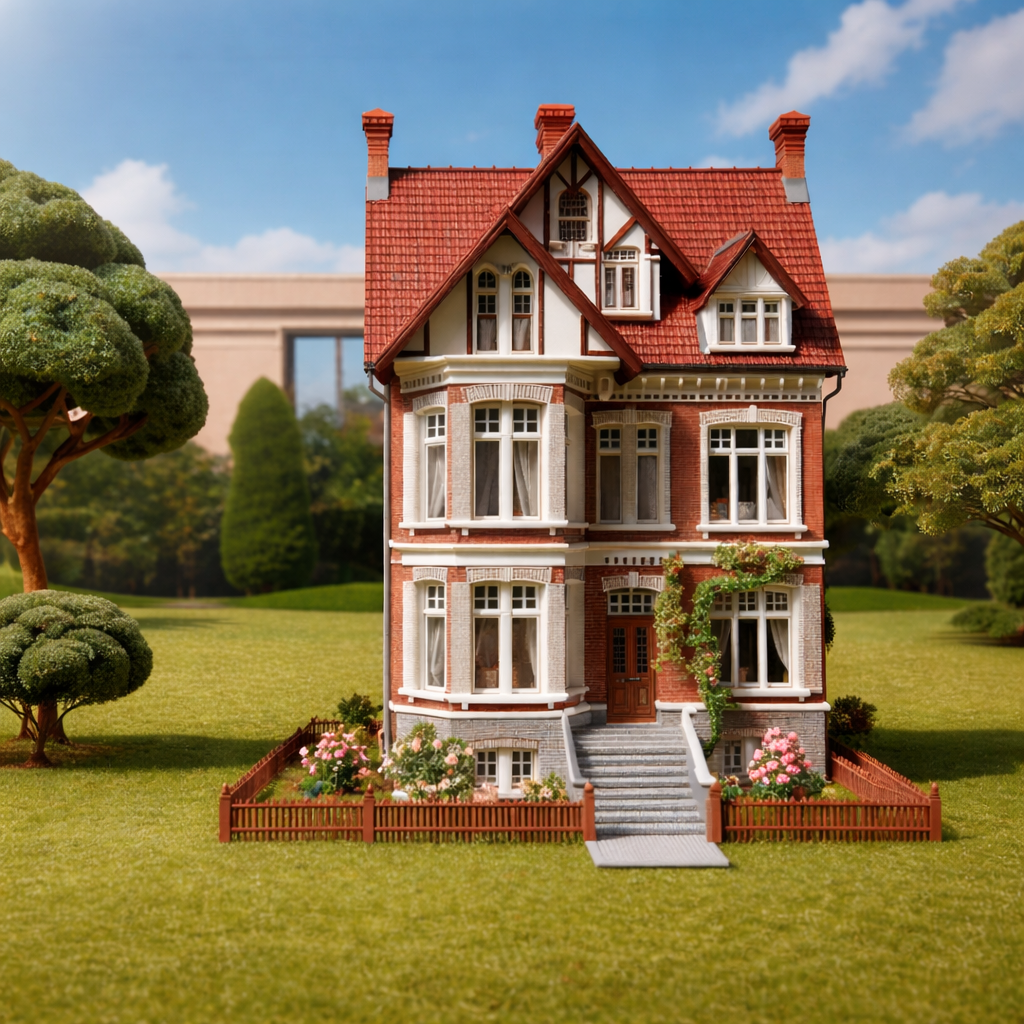
\includegraphics[width=0.7\linewidth,height=\textheight,keepaspectratio]{modules/03-introduction-to-models/../../images/fig-house.png}

}

\caption{\label{fig-house}Picture of a house}

\end{figure}%

\begin{figure}

\centering{

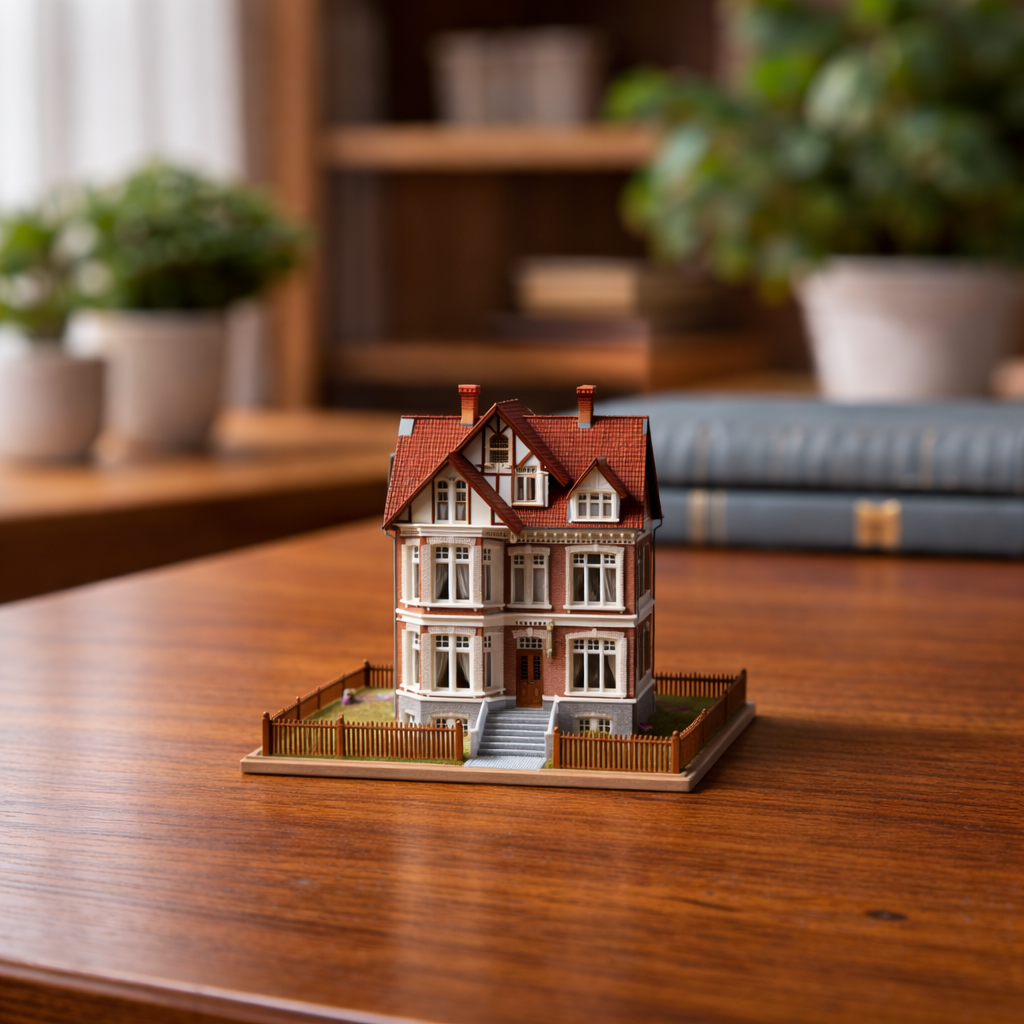
\includegraphics[width=0.7\linewidth,height=\textheight,keepaspectratio]{modules/03-introduction-to-models/../../images/fig-house-model.png}

}

\caption{\label{fig-house-model}Model of the house in
Figure~\ref{fig-house}}

\end{figure}%

Should we consider the model in Figure~\ref{fig-house-model} good? In
the words of statistician George E. P. Box, ``All models are wrong. But
some are useful for certain purposes.''

All models are wrong in the sense that they are only
\emph{representations}. However, as the miniature model of the house in
Figure~\ref{fig-house-model}, they can still be useful for some purpose.

We will be building many models in this course and should remember the
following:

\begin{itemize}
\tightlist
\item
  Models are simplifications: They inherently omit details and idealize
  reality to make complex systems manageable.
\item
  Utility over accuracy: The goal isn't perfect truth, but practical
  application and insight for a specific goal, whether it's scientific,
  business, or everyday decision-making.
\item
  Context matters: A model's usefulness depends on the purpose; a simple
  model might be great for a quick estimate, while a complex one is
  needed for detailed forecasting.
\item
  Pragmatic approach: We should focus on how wrong a model can be and
  still be helpful, rather than getting stuck on its imperfections.
\end{itemize}

How to apply this philosophy:

\begin{itemize}
\tightlist
\item
  Question your models: Continuously ask how and where a model breaks
  down.
\item
  Understand its limitations: Know the assumptions and simplifications
  behind the model.
\item
  Adapt and evolve: Be willing to refine or discard models as new
  information emerges or situations change.
\end{itemize}

\section{Mathematical models}\label{mathematical-models}

In this course, we will be building a specific kind of models --
\emph{statistical models}. However, before getting to \emph{statistical}
models, we will consider some simpler \emph{mathematical models}. The
term \emph{mathematical model} can connote many different things. Let us
clarify the sense in which we use the term. Suppose I have a data frame
\emph{homes} with data about many homes. For each home, we have its
\emph{age}, \emph{floor-area\_sqft}, \emph{number\_of\_bedrooms},
\emph{number\_of\_bathrooms}, and \emph{price}. Here are the initial
rows in the data frame.

\begin{lstlisting}[language=R]
homes |> 
  head()
\end{lstlisting}

\begin{lstlisting}
# A tibble: 6 x 5
    age floor_area_sqft number_of_bedrooms
  <dbl>           <dbl>              <dbl>
1    20            1901                  4
2    55            1614                  3
3    29            1738                  3
4    62            2137                  4
5    66            1480                  3
6     3            2492                  5
# i 2 more variables: no_of_bathrooms <dbl>,
#   price <dbl>
\end{lstlisting}

We might build a model to determine the value of \emph{price} given the
values of one or more of the other variables. In this case, let us use
the variable \emph{floor\_area\_sqft}. Remember, this is a model and so
we do not expect it be be exact. We do not aim for the model to
determine the actual \emph{price}, but only to compute a good
\emph{estimate} of the \emph{price}. (We have obviously simplified the
situation for pedagogical purposes. House prices depend on many other
factors. But that need not hold us back. You will still learn the
underlying concepts.).

What might the model look like? Equation~\ref{eq-price-model} shows the
model. \emph{For now, do not worry about how we arrived the model.}

\begin{equation}\phantomsection\label{eq-price-model}{
\widehat{\text{price}} = 61{,}399 + 394\,\text{floor\_area\_sqft}
}\end{equation}

In the model, we have placed a \emph{hat} over \emph{price} because the
model computes not the actual price of a home with the specified floor
area and instead only computes an estimate. In statistics, we place a
\emph{hat} over quantities that estimate other quantities.

Equation~\ref{eq-price-model} shows a \emph{linear} model. We call it
\emph{linear} because all variables are only raised to the fist power.
We have not squared or raised a variable to any other power. In this
course we build only \emph{linear models}.

We call the equation that Equation~\ref{eq-price-model} shows a
\textbf{model function}.

In our context, we use the term \emph{model} to denote a mathematical
equation of the kind that Equation~\ref{eq-price-model} shows. Our
models help us to determine the value of a variable in a data frame for
any given instance. Specifically, in the house price example that we
just considered, the model in Equation~\ref{eq-price-model} enables us
to estimate the \emph{price} of a home, given its floor area.

\subsection{\texorpdfstring{\emph{Response} and \emph{Explanatory}
variables}{Response and Explanatory variables}}\label{response-and-explanatory-variables}

We call the variable whose value the model estimates as the
\emph{response} variable. The variables based on which the model
estimates the \emph{response} variable are called \emph{explanatory}
variables. We can also refer to the \emph{response} variable as the
\emph{dependent} variable, and \emph{explanatory} variables as
\emph{independent} variables.

\subsection{Using the model}\label{using-the-model}

The house in the fifth row of the data frame has floor area of 1480. Its
actual price is \$553,000. What price does the model estimate? Well, we
can plug the floor area into the model -- Equation~\ref{eq-price-model}
-- and find out. If we plug it in, we get \$645,999. The model
overestimates this price.

The house in the fourteenth row of the data frame has floor area of 1293
Its actual price is \$561,000. What price does the model estimate? Well,
we can plug the floor area into the model --
Equation~\ref{eq-price-model} -- and find out. If we plug it in, we get
\$572,134. Quite close.

You should try out some more cases and wee how the model does. We will
learn a lot more about such models, including precisely measuring their
\emph{quality} as we go forward.

I won't blame you if you are wondering ``We already have the prices in
the data frame. Why do we need a model to calculate these?''

Consider again the home in the fifth row. Why did the model overestimate
the price? Well, you should consider that this particular home was not
the only one whose floor area was in the vicinity of 1480. The data set
has other homes with similar floor areas and their prices vary. If we
look at homes that have floor areas between 1430 and 1530, we see that
their prices range from \$553,000 to \$647,000. In fact, many homes
below 1480 square feet in floor area have higher prices. How could that
be? Well, variables other than floor area play a role in price too. So
our model makes an estimate based on the whole data frame.

The next section addresses two main uses of models.

\section{Purpose of a model}\label{purpose-of-a-model}

We use models in two main ways:

\begin{enumerate}
\def\labelenumi{\arabic{enumi}.}
\tightlist
\item
  \emph{Prediction}: Suppose we have built a model using the data in a
  data frame to estimate the \emph{price} of a home, given its
  \emph{floor\_area\_sqft}. We can potentially use this model to
  estimate the price of any home whose floor area we know and whose
  price we do not know -- even if this home is not in the data set.
\item
  \emph{Explanation}: Our model in Equation~\ref{eq-price-model} tells
  us that the price of a home is related to its floor area. This makes
  sense and we could have said this even without a model. However, when
  people gather data about phenomena that they do not fully understand,
  and want to understand, they often build models to understand and
  explain which variables seem to be related and in what way to a
  variable of interest.
\end{enumerate}

So, for our purposes in this course, we can define the term \emph{model}
as:

\begin{quote}
A model is a simple story we tell about data to help us summarize,
explain, or predict.
\end{quote}

You might have noted that both of the above purposes actually require us
to use a model in contexts that go outside the data that we based the
model on. When we start using models outside of the data we used to
build the model, we come face to face with the essence of statistics. We
will get to that later in the course.

\section{Average is a model too!}\label{average-is-a-model-too}

In Equation~\ref{eq-price-model}, we had a \emph{response} variable and
an \emph{explanatory} variable. What if we do not have any explanatory
variable? In the context of our home prices example, not having an
\emph{explanatory} variable is equivalent to saying:

\begin{itemize}
\tightlist
\item
  ``I have a data set of 100 homes''
\item
  ``Here are their prices''
\item
  ``I am not telling you anything else about these homes''
\item
  ``I have selected a random home from my data set''
\item
  ``Guess the price of the home I have in mind''
\end{itemize}

Based on the game we played in Chapter~\ref{sec-mean-model}, you first
compute the average of the prices as \$733,440. Your best \emph{model}
to make your guess is:

\begin{equation}\phantomsection\label{eq-avg-price-model}{
\widehat{\text{price}} = 733{,}440
}\end{equation}

That is, like in the game we played, no matter which home I choose, you
always state the average as your guess.
Equation~\ref{eq-avg-price-model} shows the \emph{model function} when
we have no

The big difference between the models in Equation~\ref{eq-price-model}
and Equation~\ref{eq-avg-price-model} is that the second one \emph{has
no explanatory variable}. When we are not given any additional helpful
information to estimate a value, our best estimate -- \emph{best model}
-- is the average!

\chapter{Visualizing Mean Models}\label{sec-visualizing-mean-models}

In the prior chapters, we have established the overall \emph{mean} as
the \emph{best model} when we have no other \emph{explanatory} variable,
and the category mean as the \emph{best model} when we have a
categorical explanatory variable.

In this chapter we use the \emph{point\_plot} function to visualize
these models.

\section{Business scenario -- fuel efficiency of vehicle
fleet}\label{business-scenario-fuel-efficiency-of-vehicle-fleet}

In Chapter~\ref{sec-mean-model}, we used a set of numbers to play a
game. Now we will extend the idea to actual data frames.

You manage a company that operates a fleet of rental cars used primarily
for city driving. The fleet includes a wide range of vehicles, from
compact sedans to larger SUVs, each with different city fuel efficiency.

For planning purposes, the company must commit to one single number to
represent the expected city fuel efficiency of a car drawn at random
from the fleet. This number is used repeatedly---for estimating fuel
costs, setting reimbursement rates, and budgeting operating expenses.

The company does not know in advance which specific car will be rented
on a given day. Some days the car will be more fuel-efficient than
expected, and on other days less fuel-efficient.

If the company assumes fuel efficiency that is too high, it
underestimates fuel costs. If it assumes fuel efficiency that is too
low, it overestimates costs and ties up capital unnecessarily. Larger
errors in either direction are more costly than smaller ones.

The decision is not evaluated based on a single rental. Instead, it is
judged by how well it performs across many rentals over time.

In this setting, the question becomes: ``What single number should the
company commit to so that total long-run cost is as small as possible?''

The data about your fleet is in the \emph{mpg} data. It has many
variables, but we focus here on the variable \emph{cty} showing us the
city miles per gallon of each car.

Assuming (artificially) that the company is only allowed to use the
variable \emph{cty} what single number should they commit to?

\subsection{Committing to one number for the entire
fleet}\label{committing-to-one-number-for-the-entire-fleet}

Based on our discussion in Chapter~\ref{sec-mean-model}, we know that
the the company should commit to the average of the variable \emph{cty}.
We can compute the average using the \emph{summarize} and \emph{mean}
functions as the code below shows.

\begin{lstlisting}[language=R]
mpg |> 
  summarize(avg_cty = mean(cty))
\end{lstlisting}

\begin{lstlisting}
# A tibble: 1 x 1
  avg_cty
    <dbl>
1    16.9
\end{lstlisting}

We can also visualize it thus:

\begin{lstlisting}[language=R]
mpg |> 
  point_plot(cty ~ 1,
             annot = "model",
             interval = "none")
\end{lstlisting}

This generates Figure~\ref{fig-cty-simple-mean-model}.

\begin{figure}

\centering{

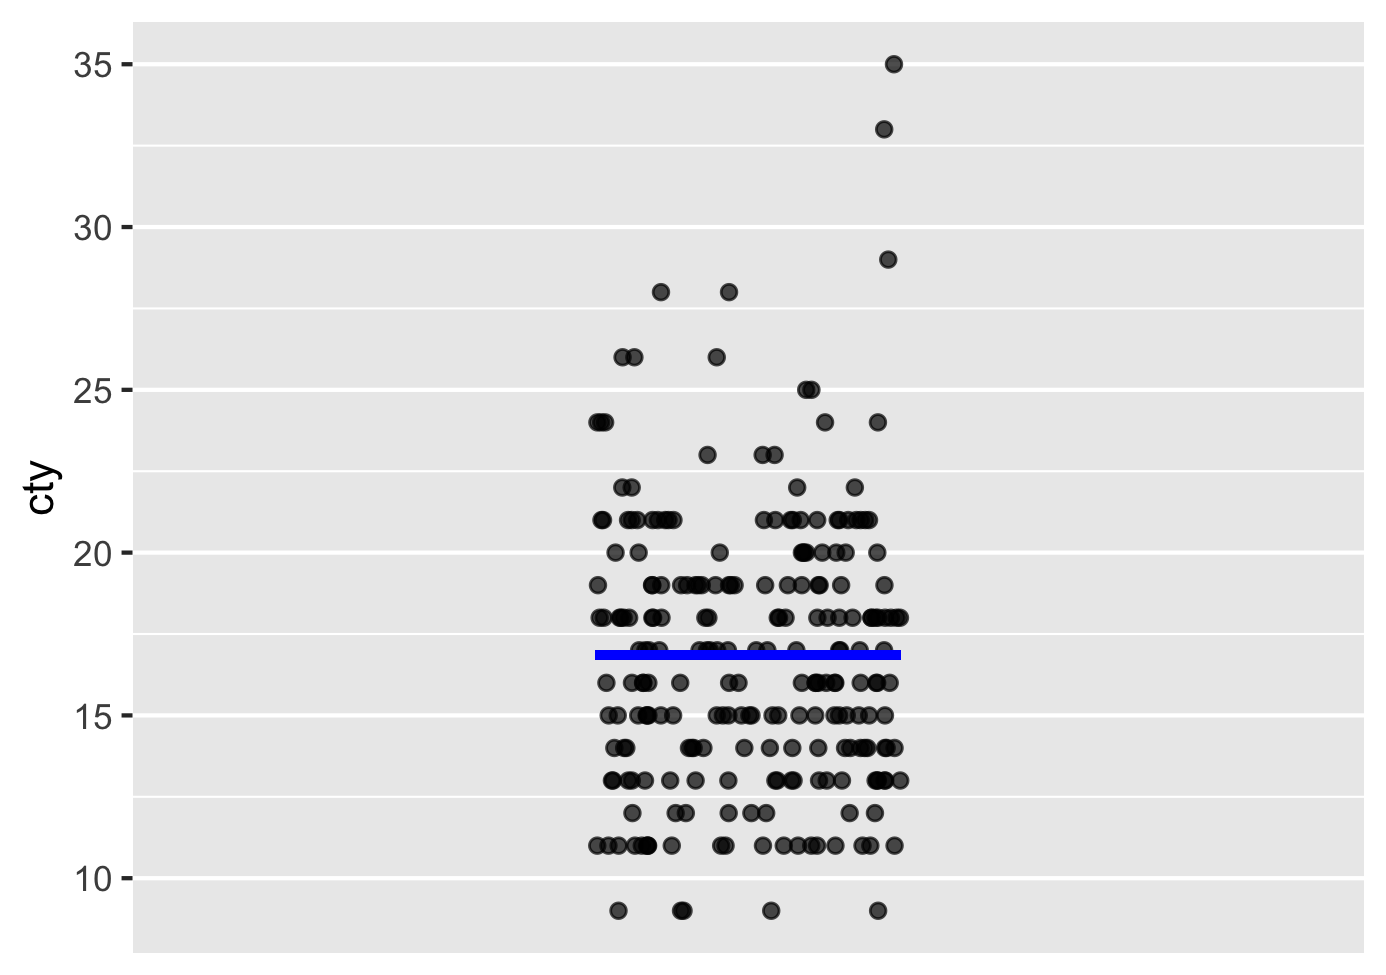
\includegraphics[width=0.7\linewidth,height=\textheight,keepaspectratio]{modules/03-introduction-to-models/../../images/fig-cty-simple-mean-model.png}

}

\caption{\label{fig-cty-simple-mean-model}Visualizing mean \emph{cty} as
the model}

\end{figure}%

The model shows the scatter plot of the points as well as a line. This
line represents the model. You can see that it falls exactly at the
average of the \emph{cty} values.

Take a look at the code:

The tilde expression

\begin{lstlisting}
cty ~ 1
\end{lstlisting}

in the code sets \emph{cty} ans=d the response variable and, by placing
1 on the RHS, shows that we have no explanatory variables.

The part

\begin{lstlisting}
annot = "model
\end{lstlisting}

Causes a \emph{model} to be visualized as well. We know that the mean is
our model and this plot visualizes it by drawing a line at the average
\emph{cty}.

For now, you can ignore:

\begin{lstlisting}
interval = "none"
\end{lstlisting}

So, if we have to commit to one number as our estimate for the city
mileage irrespective of other details about a car like its \emph{class},
\emph{drv} or anything else, our best commitment is to the overall
average. As we have seen in Chapter~\ref{sec-models-intro}, this is a
model with just a response variable and no explanatory variables. We can
write it as Equation~\ref{eq-cty-model}.

\begin{equation}\phantomsection\label{eq-cty-model}{
\widehat{\text{cty}} = 16.9
}\end{equation}

We placed a \emph{hat} on \emph{cty} because this is just an estimate or
a model value and not an actual data point.

\section{We can do better with more
information}\label{we-can-do-better-with-more-information}

Instead of having to commit to one single number for the fuel efficiency
for the entire fleet, what if we could use a different number for each
class of vehicle? In out \emph{mpg} data set, we have vehicles of
different classes -- variable \emph{class}. This has values like
\emph{Compact}, \emph{SUV} and \emph{Pickup truck}.

Based on Chapter~\ref{sec-category-means}, we know that for each class
of vehicle, we should commit to the average of \emph{cty} for that
class.

We can compute these averages easily:

\begin{lstlisting}[language=R]
mpg |> 
  summarize(avg_cty = mean(cty), .by = class)
\end{lstlisting}

\begin{lstlisting}
# A tibble: 7 x 2
  class      avg_cty
  <chr>        <dbl>
1 compact       20.1
2 midsize       18.8
3 suv           13.5
4 2seater       15.4
5 minivan       15.8
6 pickup        13  
7 subcompact    20.4
\end{lstlisting}

Note how the above code is very similar to what we would use for
computing the overall average, but we have added:

\begin{lstlisting}
.by = class
\end{lstlisting}

To show that we do not want just one average for the whole data frame,
but we want separate averages for each \emph{class} of vehicle. As
simple as that!

Let us visualize this model:

\begin{lstlisting}[language=R]
mpg |> 
  point_plot(cty ~ class, annot = "model",
             interval = "none")
\end{lstlisting}

Figure~\ref{fig-cty-class-model} shows the model visualization.

\begin{figure}

\centering{

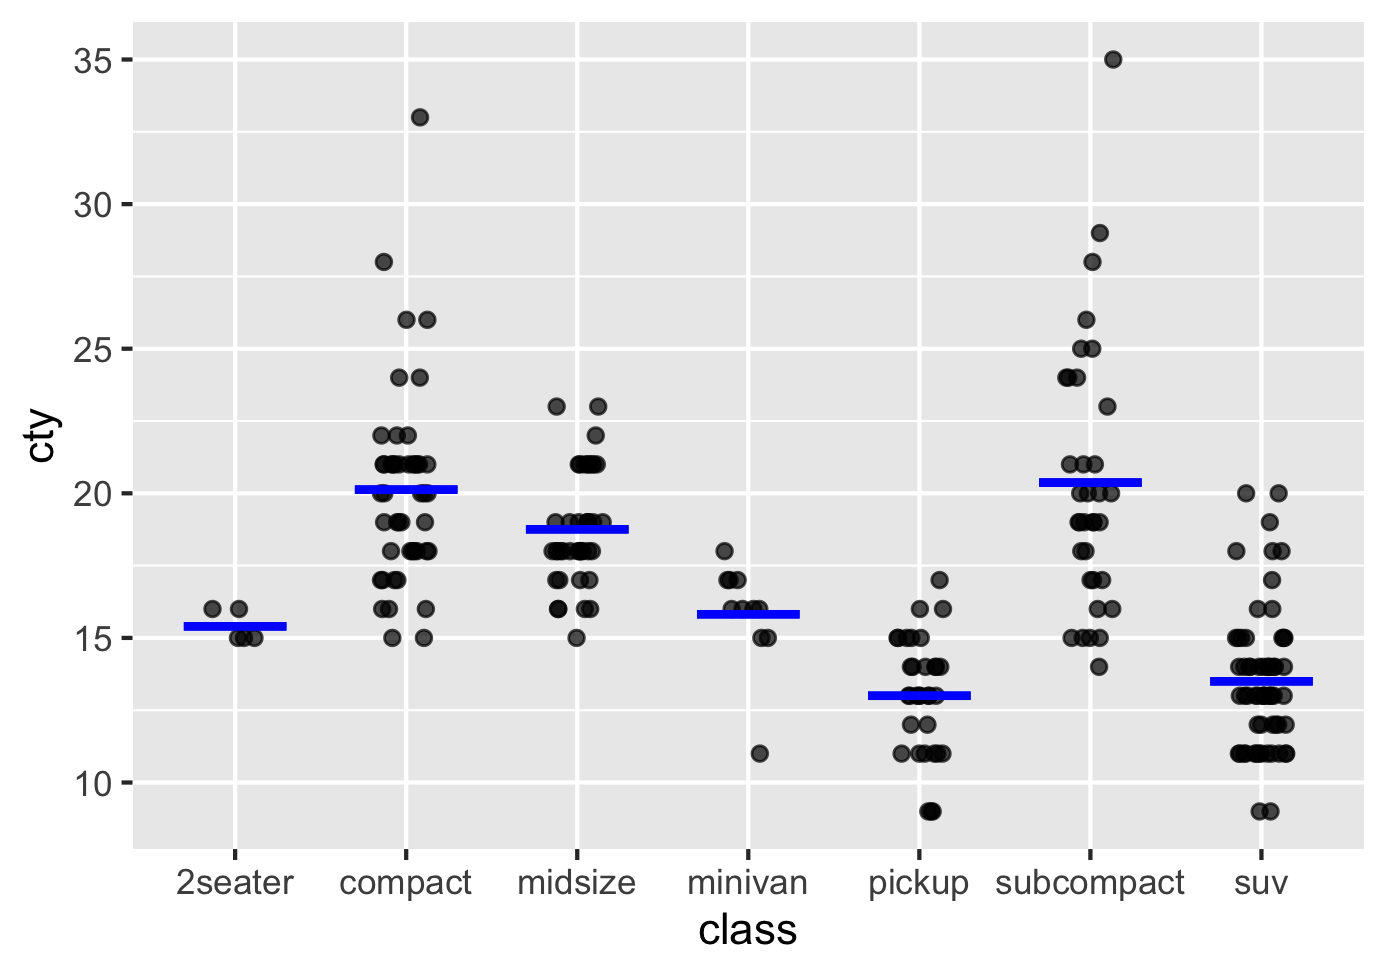
\includegraphics[width=0.7\linewidth,height=\textheight,keepaspectratio]{modules/03-introduction-to-models/../../images/fig-cty-class-model.png}

}

\caption{\label{fig-cty-class-model}Visualizing the more sophisticated
model of mean \emph{cty} by \emph{class} as the model when we have
\emph{class} as an explanatory variable}

\end{figure}%

How do we express this model as an equation like we did with
Equation~\ref{eq-cty-model}?

Equation~\ref{eq-cty-class-model} shows the model as an equation.

\begin{equation}\phantomsection\label{eq-cty-class-model}{
\widehat{\text{cty}} =
\begin{cases}
20.1 & \text{if } \text{class} = \text{"compact"} \\
18.8 & \text{if } \text{class} = \text{"midsize"} \\
13.5 & \text{if } \text{class} = \text{"SUV"} \\
15.4 & \text{if } \text{class} = \text{"2seater"} \\
15.8 & \text{if } \text{class} = \text{"minivan"} \\
13.0 & \text{if } \text{class} = \text{"pickup"} \\
20.4 & \text{if } \text{class} = \text{"subcompact"}
\end{cases}
}\end{equation}

Instead of class, we can have \emph{drv} as the explanatory variable as
well. Here are code snippets that will compute the model and plot it.

\begin{lstlisting}[language=R]
mpg |> 
  summarize(avg_cty = mean(cty), .by = drv)
\end{lstlisting}

\begin{lstlisting}
# A tibble: 3 x 2
  drv   avg_cty
  <chr>   <dbl>
1 f        20.0
2 4        14.3
3 r        14.1
\end{lstlisting}

Note that we only had to change the .by to reflect that we are now
computing averages by \emph{drv}.

\begin{lstlisting}[language=R]
mpg |> 
  point_plot(cty ~ drv, annot = "model",
             interval = "none")
\end{lstlisting}

We just changed the RHS of the tilde expression to \emph{drv} instead of
\emph{class}.

Figure~\ref{fig-cty-drv-model} shows the visualization.

\begin{figure}

\centering{

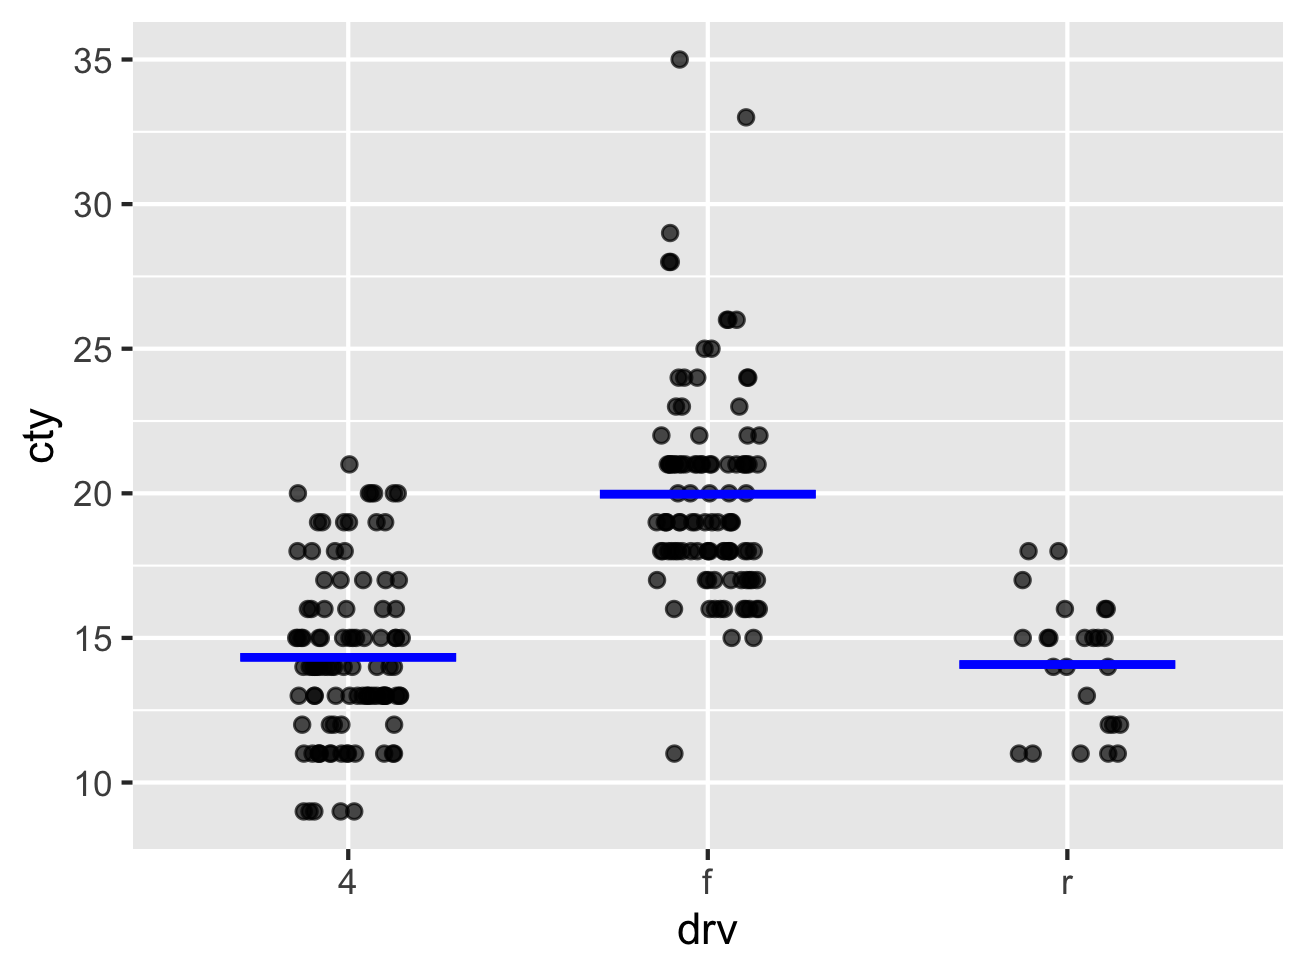
\includegraphics[width=0.7\linewidth,height=\textheight,keepaspectratio]{modules/03-introduction-to-models/../../images/fig-cty-drv-model.png}

}

\caption{\label{fig-cty-drv-model}Visualizing the model of mean
\emph{cty} by \emph{drv} as the model when we have \emph{drv} as an
explanatory variable}

\end{figure}%

Equation~\ref{eq-cty-drv-model} shows the model in equation form.

\begin{equation}\phantomsection\label{eq-cty-drv-model}{
\widehat{\text{cty}} =
\begin{cases}
20.0 & \text{if } \text{drv} = \text{"f"} \\
14.3 & \text{if } \text{drv} = \text{"4"} \\
14.1 & \text{if } \text{drv} = \text{"r"} \\
\end{cases}
}\end{equation}

The \emph{mpg} data frame has another column \emph{fl} to represent the
fuel type of the vehicle. We now want to use \emph{fl} as the
explanatory variable. Try out the following using the above as examples.

\begin{itemize}
\tightlist
\item
  Write R code to compute the average of \emph{cty} for each fuel type
\item
  Write R code to visualize the model with \emph{cty} as the response
  variable and \emph{fl} as the explanatory variable.
\item
  Write out the model equation for this scenario.
\end{itemize}

\part{More on models -- least squares}

\chapter*{Module 4: Linear Regression
Models}\label{module-4-linear-regression-models}
\addcontentsline{toc}{chapter}{Module 4: Linear Regression Models}

\markboth{Module 4: Linear Regression Models}{Module 4: Linear
Regression Models}

This module fills in the details on top of the intuitive foundation for
a linear model that the previous module laid.It introduces the idea of
the least squares best fit line and its corresponding model. The module
covers R code for building linear models for the case of a single
numerical explanatory variable, a single categorical variable and a
combination of one numerical and one categorical explanatory variable.It
shows how to distill the model function based on the regression output.

\section*{Learning Goals}\label{learning-goals-3}
\addcontentsline{toc}{section}{Learning Goals}

\markright{Learning Goals}

\begin{itemize}
\tightlist
\item
  a
\item
  b
\item
  c
\end{itemize}

\section*{Structure of This Module}\label{structure-of-this-module-3}
\addcontentsline{toc}{section}{Structure of This Module}

\markright{Structure of This Module}

\begin{itemize}
\tightlist
\item
  mention that the model gives an estimated value, but defer detailed
  discussion until later
\item
  R code for building model with no explanatory variable and
  reconstructing the model function
\item
  R code for building model with one numeric explanatory variable and
  reconstructing the model function
\item
  R code for building model with one numeric explanatory variable and
  one categorical explanatory variable and reconstructing the model
  function
\end{itemize}

\chapter{Line of Best Fit}\label{sec-best-fit-line}

In prior chapters we have looked at the situation when we have a
numerical response variable and either no explanatory variable or a
single categorical explanatory variable. In this chapter we look at the
important case when the response variable and the explanatory variable
are numerical.

In our running story, this is the third meeting of our interns with
Amanda who owns a business that operates kiosks in a city at two
locations. Last month, the interns used kiosk labels to help set
different staffing levels for the Beach and the Mall.

Now Amanda brings a new kind of hint.

``It's not just location that seems to affect the number of customers we
get.'' she says. ``Today, I need you all to help me with a decision for
the beach kiosk. At the Beach kiosk, demand seems to swing with
temperature. I want a model that uses what we know \emph{today} about
tomorrow's temperature (the forecast) to predict customer traffic for
tomorrow. This time, I will use the prediction not for staffing, but to
decide on stock levels of items. We do not want to under or overstock
too much and so good predictions can really help me.''

She adds one constraint immediately:

``Keep it simple. I need something I can explain in one sentence.''

In this chapter, we continue our model-building journey. A model is
simply a rule that takes information we have and produces a predicted
value for the response.

\begin{itemize}
\item
  With no explanatory variable, we learned in
  Chapter~\ref{sec-mean-model}, that our model is ``always predict the
  mean.''
\item
  With a single categorical explanatory variable,
  Chapter~\ref{sec-category-means} showed us that our model should be
  ``predict the mean of the category.''
\end{itemize}

\begin{tcolorbox}[enhanced jigsaw, colback=white, leftrule=.75mm, toprule=.15mm, bottomtitle=1mm, breakable, coltitle=black, toptitle=1mm, title=\textcolor{quarto-callout-note-color}{\faInfo}\hspace{0.5em}{Quick Check}, opacitybacktitle=0.6, colbacktitle=quarto-callout-note-color!10!white, arc=.35mm, left=2mm, colframe=quarto-callout-note-color-frame, titlerule=0mm, rightrule=.15mm, bottomrule=.15mm, opacityback=0]

When we use the mean as a model, what value do we predict for every
observation?

Why is this considered a model rather than just a summary?

\end{tcolorbox}

\begin{tcolorbox}[enhanced jigsaw, colback=white, leftrule=.75mm, toprule=.15mm, bottomtitle=1mm, breakable, coltitle=black, toptitle=1mm, title=\textcolor{quarto-callout-note-color}{\faInfo}\hspace{0.5em}{Answer}, opacitybacktitle=0.6, colbacktitle=quarto-callout-note-color!10!white, arc=.35mm, left=2mm, colframe=quarto-callout-note-color-frame, titlerule=0mm, rightrule=.15mm, bottomrule=.15mm, opacityback=0]

The model predicts the same value---the mean---for every observation.

It is a model because it provides a rule for generating predicted
values, not just a numerical description of the data.

\end{tcolorbox}

\begin{tcolorbox}[enhanced jigsaw, colback=white, leftrule=.75mm, toprule=.15mm, bottomtitle=1mm, breakable, coltitle=black, toptitle=1mm, title=\textcolor{quarto-callout-note-color}{\faInfo}\hspace{0.5em}{Quick Check}, opacitybacktitle=0.6, colbacktitle=quarto-callout-note-color!10!white, arc=.35mm, left=2mm, colframe=quarto-callout-note-color-frame, titlerule=0mm, rightrule=.15mm, bottomrule=.15mm, opacityback=0]

How does a category-mean model improve on the overall mean model?

What additional information does it use?

\end{tcolorbox}

\begin{tcolorbox}[enhanced jigsaw, colback=white, leftrule=.75mm, toprule=.15mm, bottomtitle=1mm, breakable, coltitle=black, toptitle=1mm, title=\textcolor{quarto-callout-note-color}{\faInfo}\hspace{0.5em}{Answer}, opacitybacktitle=0.6, colbacktitle=quarto-callout-note-color!10!white, arc=.35mm, left=2mm, colframe=quarto-callout-note-color-frame, titlerule=0mm, rightrule=.15mm, bottomrule=.15mm, opacityback=0]

A category-mean model allows different predictions for different groups.

It improves on the overall mean model by using information about group
membership instead of treating all observations as identical.

\end{tcolorbox}

In this chapter we consider a single numerical explanatory variable. In
this case we need something quite different.

\section{The beach kiosk staffing
problem}\label{the-beach-kiosk-staffing-problem}

We again consider a situation where the company gets a hint before
making a decision---but now the hint is numerical, not categorical.

Amanda is focused on the Beach kiosk. (The Mall kiosk is steadier, but
the Beach kiosk shas more variance in daily customer numbers and so just
using the average can be costly.

Management has noticed that customer traffic at the Beach kiosk varies
strongly with the day's high temperature.

Over many past days, the company has recorded:

\begin{itemize}
\item
  the day's high temperature (in °F), and
\item
  the number of customers who visited the beach kiosk that day.
\end{itemize}

Let us assume that data are available for 25 different days. (As before,
for understanding the ideas, the exact number of days is not important.)

Table~\ref{tbl-temp-customers} shows the historical data.

\begin{longtable}[]{@{}lrr@{}}
\caption{Daily temperature and customer
counts}\label{tbl-temp-customers}\tabularnewline
\toprule\noalign{}
day & temperature & customers \\
\midrule\noalign{}
\endfirsthead
\toprule\noalign{}
day & temperature & customers \\
\midrule\noalign{}
\endhead
\bottomrule\noalign{}
\endlastfoot
D01 & 58 & 98 \\
D02 & 60 & 104 \\
D03 & 62 & 122 \\
D04 & 64 & 113 \\
D05 & 66 & 117 \\
D06 & 68 & 133 \\
D07 & 70 & 126 \\
D08 & 72 & 115 \\
D09 & 74 & 123 \\
D10 & 76 & 128 \\
D11 & 78 & 145 \\
D12 & 80 & 141 \\
D13 & 58 & 106 \\
D14 & 60 & 107 \\
D15 & 62 & 105 \\
D16 & 64 & 127 \\
D17 & 66 & 120 \\
D18 & 68 & 103 \\
D19 & 70 & 128 \\
D20 & 72 & 121 \\
D21 & 74 & 120 \\
D22 & 76 & 130 \\
D23 & 78 & 127 \\
D24 & 80 & 132 \\
D25 & 58 & 98 \\
\end{longtable}

Based this, the company must decide how many customers will show up
tomorrow. They will u8se that to determine how much of each item to
stock for sale. It can use an extremely reliable temperature forecast
for its city.

The problem now is this:

\begin{quote}
Given the forecast high temperature for a day, how many customers should
the company plan for?
\end{quote}

\subsection{How does this differ from earlier examples we have
studied?}\label{how-does-this-differ-from-earlier-examples-we-have-studied}

In Chapter~\ref{sec-mean-model}, we used no hints at all, and the mean
turned out to be the best model.

In Chapter~\ref{sec-category-means}, our hint was categorical, and the
mean within each category turned out to be the best model.

This time, the situation is fundamentally different. Our hint,
temperature, is numerical, and so none of the earlier ``mean-based''
approaches applies directly.

One possibility would be to convert temperature into categories such as
\emph{Cold}, \emph{Warm}, and \emph{Hot}, and then apply the
category-means approach. While this would work, it is somewhat
artificial. Two days that differ by only one degree could end up in
different categories. For example, calling 50°F Cold and 51°F Warm
introduces an arbitrary cutoff that has no real business justification.

Temperature does not naturally fall into clear bins. Can we do better?

\subsection{Toward a rule-based model}\label{toward-a-rule-based-model}

Rather than assigning a few separate numbers, Amanda now wants a rule
that:

\begin{quote}
takes the day's temperature as input and produces an estimated number of
customers as output.
\end{quote}

Many such rules are possible. The company wants a simple rule that takes
a temperature as input and produces a predicted number of customers as
output. Let us assume that the same general pattern will continue for
temperatures. It is not going to be exactly the same, but the general
range and the distribution will remain the same for the next month.
Therefore, if we applied our model to the data set in
Table~\ref{tbl-temp-customers}, its output should reasonably match the
actual number of customers in the data set.

Figure~\ref{fig-beach-kiosk-model-box-diagram} shows what Amanda is
looking for at a high level.

\begin{figure}

\centering{

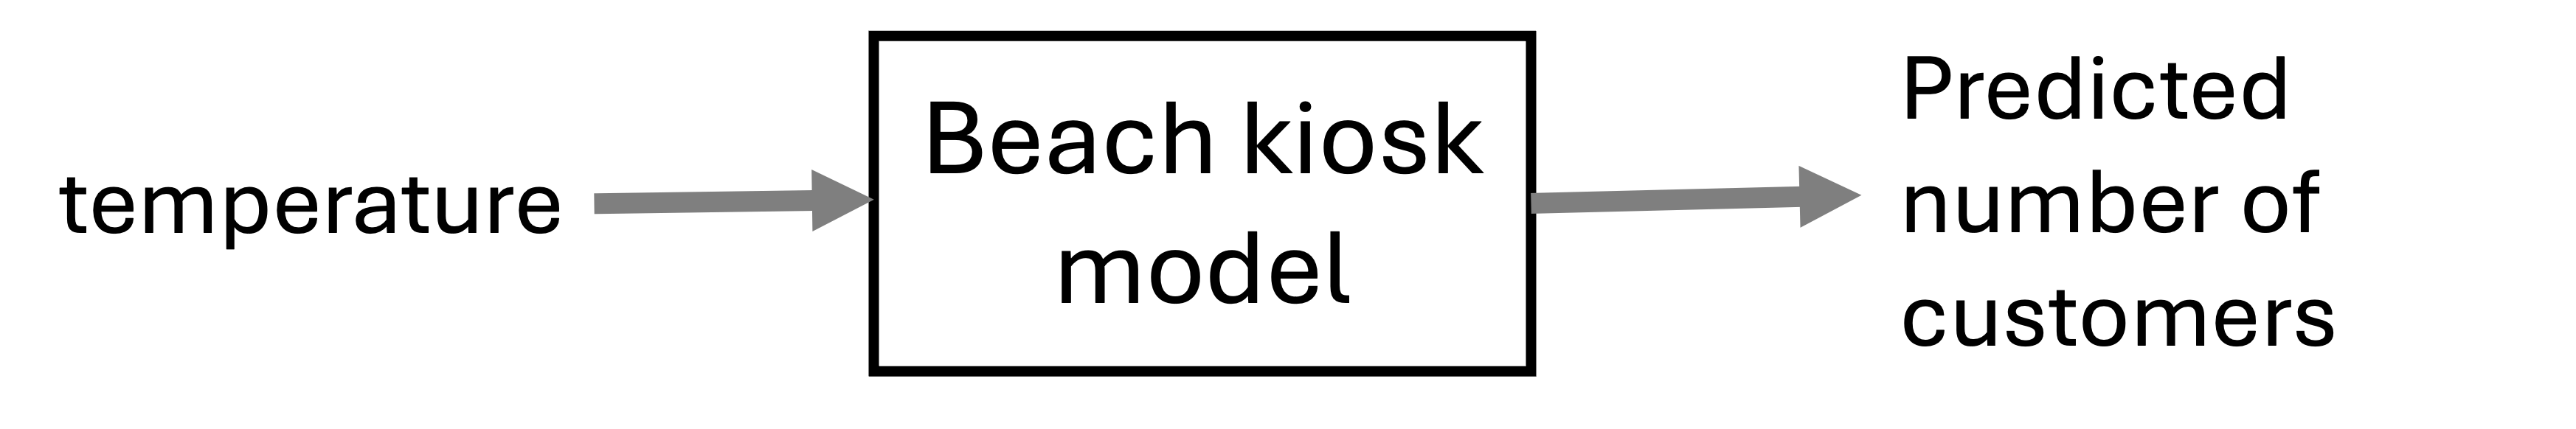
\includegraphics[width=0.7\linewidth,height=\textheight,keepaspectratio]{modules/04-more-on-models/../../images/fig-beach-kiosk-model-box-diagram.png}

}

\caption{\label{fig-beach-kiosk-model-box-diagram}Model that takes a
temperature as input and produces a predicted number of customers for
the beach kiosk -- the model should be based on the data in
Table~\ref{tbl-temp-customers}}

\end{figure}%

We know that with higher temperatures more people will hit the beach.

Peter has an idea. ``Since Amanda is looking for a simple rule, should
we consider consider a model which looks something like this?'' He draws
a picture. Figure~\ref{fig-specific-beach-kiosk-model-box}). ``Of
course, I just made up the numbers 15 and 2. With this model, if we
input a temperature of 70, the model will predict 155 customers.''

\begin{figure}

\centering{

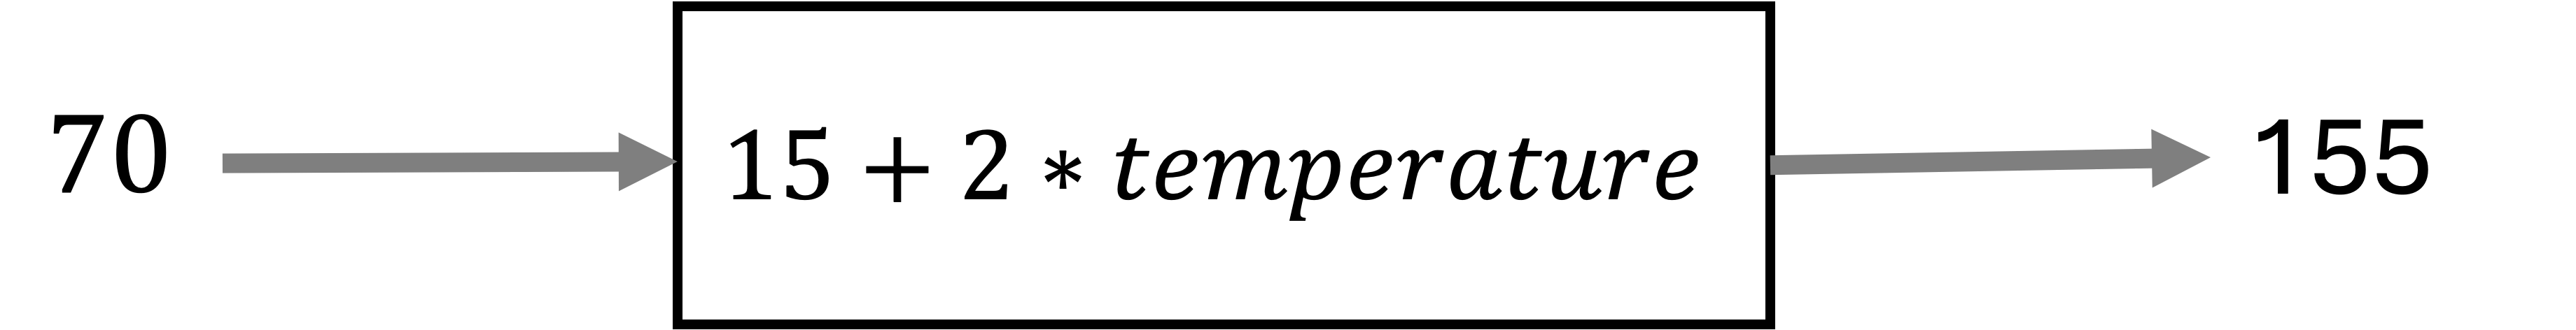
\includegraphics[width=0.7\linewidth,height=\textheight,keepaspectratio]{modules/04-more-on-models/../../images/fig-specific-beach-kiosk-model-box.png}

}

\caption{\label{fig-specific-beach-kiosk-model-box}Peter's example model
for a model to estimate customers based on temperature}

\end{figure}%

Peter further clarifies ``I did not mean the specific numbers 15 and 2
literally in Figure~\ref{fig-specific-beach-kiosk-model-box}, I am
really saying that we could look for a model that has the general form
in this figure'' and he quickly sketches
Figure~\ref{fig-beach-kiosk-temp-generic-model}

``We just need to find \emph{good} values for \emph{a} and \emph{b}.

\begin{figure}

\centering{

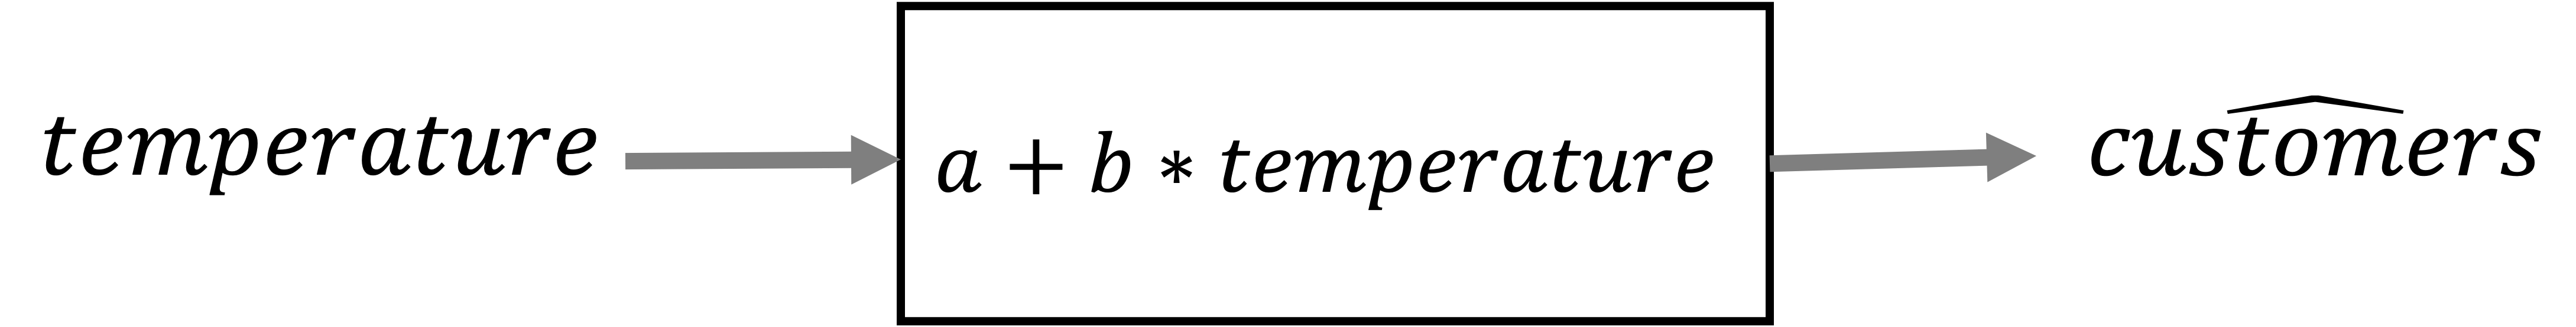
\includegraphics[width=0.7\linewidth,height=\textheight,keepaspectratio]{modules/04-more-on-models/../../images/fig-beach-kiosk-temp-generic-model.png}

}

\caption{\label{fig-beach-kiosk-temp-generic-model}Peter's second
explanatory sketch showing that he wants a model of this general form,
but wants to find good values for \emph{a} and \emph{b} so that the
model generates good predictions}

\end{figure}%

Peter then writes Equation~\ref{eq-kiosk-cust-temp-model} to explain the
same idea and adds ``I placed a \emph{hat} on top of \emph{customers}
because the equation only calculates an \emph{estimate} and this could
be different from an actual value.''

\begin{equation}\phantomsection\label{eq-kiosk-cust-temp-model}{
\widehat{\text{customers}} = a +  b\times\text{temperature}
}\end{equation}

\begin{tcolorbox}[enhanced jigsaw, colback=white, leftrule=.75mm, toprule=.15mm, bottomtitle=1mm, breakable, coltitle=black, toptitle=1mm, title=\textcolor{quarto-callout-important-color}{\faExclamation}\hspace{0.5em}{Important}, opacitybacktitle=0.6, colbacktitle=quarto-callout-important-color!10!white, arc=.35mm, left=2mm, colframe=quarto-callout-important-color-frame, titlerule=0mm, rightrule=.15mm, bottomrule=.15mm, opacityback=0]

Peter has proposed a specific form of model from an \textbf{infinite}
number of possible models. For example, the model could have taken any
of the following forms. Each of them allows us to plug in a temperature
and get an estimate for the number of customers, provided we fix some
actual values for \emph{a}, \emph{b}, \emph{c}, \emph{x}, \emph{y} and
\emph{z}.

\begin{equation}\phantomsection\label{eq-linear-model-form}{
\widehat{\text{customers}} = a +  b\times\text{temperature}^2
}\end{equation}

\[
\widehat{\text{customers}} = a + b\times\text{temperature} + c\times\text{temperature}^2
\]

\[
\widehat{\text{customers}} =
\begin{cases}
a & \text{if } \text{temperature} \leq x \\
b & \text{if } x < \text{temperature} \leq y \\
c & \text{if } \text{temperature} > y
\end{cases}
\]

\ldots{} and a model does not even have to have a mathematical form like
the ones above. \textbf{Any method that can take a \emph{temperature} as
input and produce an estimated number of customers can be a model}.

\end{tcolorbox}

\begin{tcolorbox}[enhanced jigsaw, colback=white, leftrule=.75mm, toprule=.15mm, bottomtitle=1mm, breakable, coltitle=black, toptitle=1mm, title=\textcolor{quarto-callout-important-color}{\faExclamation}\hspace{0.5em}{Important}, opacitybacktitle=0.6, colbacktitle=quarto-callout-important-color!10!white, arc=.35mm, left=2mm, colframe=quarto-callout-important-color-frame, titlerule=0mm, rightrule=.15mm, bottomrule=.15mm, opacityback=0]

In many business and social science situations, we prefer \emph{linear}
models like Equation~\ref{eq-linear-model-form}. In this course, we only
study linear models.

Fields like \emph{machine learning} consider many other types of models.

\end{tcolorbox}

Angela says ``That's a great idea Peter! Amanda wanted something simple.
Of course we gave her very simple models earlier too, but now we have to
incorporate \emph{temperature} and I cannot imagine something that
adjusts its predictions to the temperature and is simpler than what
Peter has shown.''

``If we fix the values of \emph{a} and \emph{b},
Equation~\ref{eq-kiosk-cust-temp-model} produces a predicted number of
customers for any temperature. For example, if we fix a value of 15 for
\emph{a} and 2 for \emph{b} as Peter did before, then
Equation~\ref{eq-kiosk-cust-temp-model-specific} shows our model to
determine the number of customers for any temperature. If we plug in a
temperature of 70, the model will give us 155 as the estimated number of
customers.''

\begin{equation}\phantomsection\label{eq-kiosk-cust-temp-model-specific}{
\widehat{\text{customers}} = 15 +  2\times\text{temperature}
}\end{equation}

Igor says ``I like this idea too. Its prediction changes smoothly as
temperature changes, and it avoids arbitrary cutoffs.''

Dave sounds a cautionary note ``This is all great guys, but how do we
find the \emph{best} values for \emph{a} and \emph{b}? And what do we
mean by \emph{good} choices?''

Suzie: ``I have an idea about how we might define \emph{good}. Suppose
we have a model -- let us say for the time being that we use
Equation~\ref{eq-kiosk-cust-temp-model-specific}. That is, given any
temperature, we plug it into
Equation~\ref{eq-kiosk-cust-temp-model-specific} and it spits out the
estimated number of customers.

Suppose we plug in 66 for temperature.
Equation~\ref{eq-kiosk-cust-temp-model-specific} says the number of
customers is 15 + 2*66, or 147. In our data, the number of customers for
66 degrees is 117 for one of the rows where the temperature is 66. So
the model's estimate is off by 30.''

David's eyes light up ``Oh, we can treat this just like we did earlier
and get the penalty by squaring!. This penalty will become 30*30, or 900
for that one row.''

Igor then observes ``For any given value of \emph{a} and \emph{b}, we
can compute the penalty corresponding to each row of the data. With
\emph{a} = 15 and \emph{b} = 2, we can compute the penalties for each
row.'' He then worked for a few minutes to come up with penalties for
all the rows of Table~\ref{tbl-temp-customers} and came up with
Table~\ref{tbl-igor-computations-for-15-2}.

\begin{longtable}[]{@{}
  >{\raggedright\arraybackslash}p{(\linewidth - 10\tabcolsep) * \real{0.0755}}
  >{\raggedleft\arraybackslash}p{(\linewidth - 10\tabcolsep) * \real{0.2264}}
  >{\raggedleft\arraybackslash}p{(\linewidth - 10\tabcolsep) * \real{0.1887}}
  >{\raggedleft\arraybackslash}p{(\linewidth - 10\tabcolsep) * \real{0.2642}}
  >{\raggedleft\arraybackslash}p{(\linewidth - 10\tabcolsep) * \real{0.0943}}
  >{\raggedleft\arraybackslash}p{(\linewidth - 10\tabcolsep) * \real{0.1509}}@{}}
\caption{Igor's computations: For each row he plugged in the temperature
into Equation~\ref{eq-kiosk-cust-temp-model-specific} and computed
\(\widehat{\text{customers}}\) and then computed the squared difference
between the actual value of \emph{customers} and
\(\widehat{\text{customers}}\)}\label{tbl-igor-computations-for-15-2}\tabularnewline
\toprule\noalign{}
\begin{minipage}[b]{\linewidth}\raggedright
day
\end{minipage} & \begin{minipage}[b]{\linewidth}\raggedleft
temperature
\end{minipage} & \begin{minipage}[b]{\linewidth}\raggedleft
customers
\end{minipage} & \begin{minipage}[b]{\linewidth}\raggedleft
\(\widehat{\text{customers}}\)
\end{minipage} & \begin{minipage}[b]{\linewidth}\raggedleft
diff
\end{minipage} & \begin{minipage}[b]{\linewidth}\raggedleft
penalty
\end{minipage} \\
\midrule\noalign{}
\endfirsthead
\toprule\noalign{}
\begin{minipage}[b]{\linewidth}\raggedright
day
\end{minipage} & \begin{minipage}[b]{\linewidth}\raggedleft
temperature
\end{minipage} & \begin{minipage}[b]{\linewidth}\raggedleft
customers
\end{minipage} & \begin{minipage}[b]{\linewidth}\raggedleft
\(\widehat{\text{customers}}\)
\end{minipage} & \begin{minipage}[b]{\linewidth}\raggedleft
diff
\end{minipage} & \begin{minipage}[b]{\linewidth}\raggedleft
penalty
\end{minipage} \\
\midrule\noalign{}
\endhead
\bottomrule\noalign{}
\endlastfoot
D01 & 58 & 98 & 131 & -33 & 1089 \\
D02 & 60 & 104 & 135 & -31 & 961 \\
D03 & 62 & 122 & 139 & -17 & 289 \\
D04 & 64 & 113 & 143 & -30 & 900 \\
D05 & 66 & 117 & 147 & -30 & 900 \\
D06 & 68 & 133 & 151 & -18 & 324 \\
D07 & 70 & 126 & 155 & -29 & 841 \\
D08 & 72 & 115 & 159 & -44 & 1936 \\
D09 & 74 & 123 & 163 & -40 & 1600 \\
D10 & 76 & 128 & 167 & -39 & 1521 \\
D11 & 78 & 145 & 171 & -26 & 676 \\
D12 & 80 & 141 & 175 & -34 & 1156 \\
D13 & 58 & 106 & 131 & -25 & 625 \\
D14 & 60 & 107 & 135 & -28 & 784 \\
D15 & 62 & 105 & 139 & -34 & 1156 \\
D16 & 64 & 127 & 143 & -16 & 256 \\
D17 & 66 & 120 & 147 & -27 & 729 \\
D18 & 68 & 103 & 151 & -48 & 2304 \\
D19 & 70 & 128 & 155 & -27 & 729 \\
D20 & 72 & 121 & 159 & -38 & 1444 \\
D21 & 74 & 120 & 163 & -43 & 1849 \\
D22 & 76 & 130 & 167 & -37 & 1369 \\
D23 & 78 & 127 & 171 & -44 & 1936 \\
D24 & 80 & 132 & 175 & -43 & 1849 \\
D25 & 58 & 98 & 131 & -33 & 1089 \\
\end{longtable}

Angela says: ``Well the total penalty is 28,312. How do we know if
different values for \emph{a} and \emph{b} can give us a lower penalty?
In earlier weeks we only had to try different values for one thing. Here
we have two things \emph{a} and \emph{b} to think about. What do we
do?''

Suzie says: ``But we have made progress. We have at least clearly
defined the problem. We need to find the values for \emph{a} and
\emph{b} that will give us the lowest possible total penalty along the
lines of Igor's Table~\ref{tbl-igor-computations-for-15-2}. That is, we
try many different values for \&\emph{a} and \emph{b} and compute Igor's
table (Table~\ref{tbl-igor-computations-for-15-2}) for that combination.
We then select the combination that produces the lowest total penalty.
We want the lowest total penalty because that will mean that we have got
the model estimates as close as we can to the real values in the data.''

Peter says ``Hey, this reminds me of something I saw my dad doing for
his work. He always says that visualizing makes things easier. Why don't
we try that first?''\,''

\section{Visualizing the model}\label{visualizing-the-model}

Peter continues: ``Graphically,
Equation~\ref{eq-kiosk-cust-temp-model-specific} represents a straight
line. Let us generate a scatterplot of the data first.'' He writes come
code and generates Figure~\ref{fig-kiosk-temp-cust-scatter} which shows
the relationship between \emph{temperature} and \emph{customers}.

\begin{lstlisting}[language=R]
kiosk |> 
  point_plot(customers ~ temperature)
\end{lstlisting}

\begin{figure}

\centering{

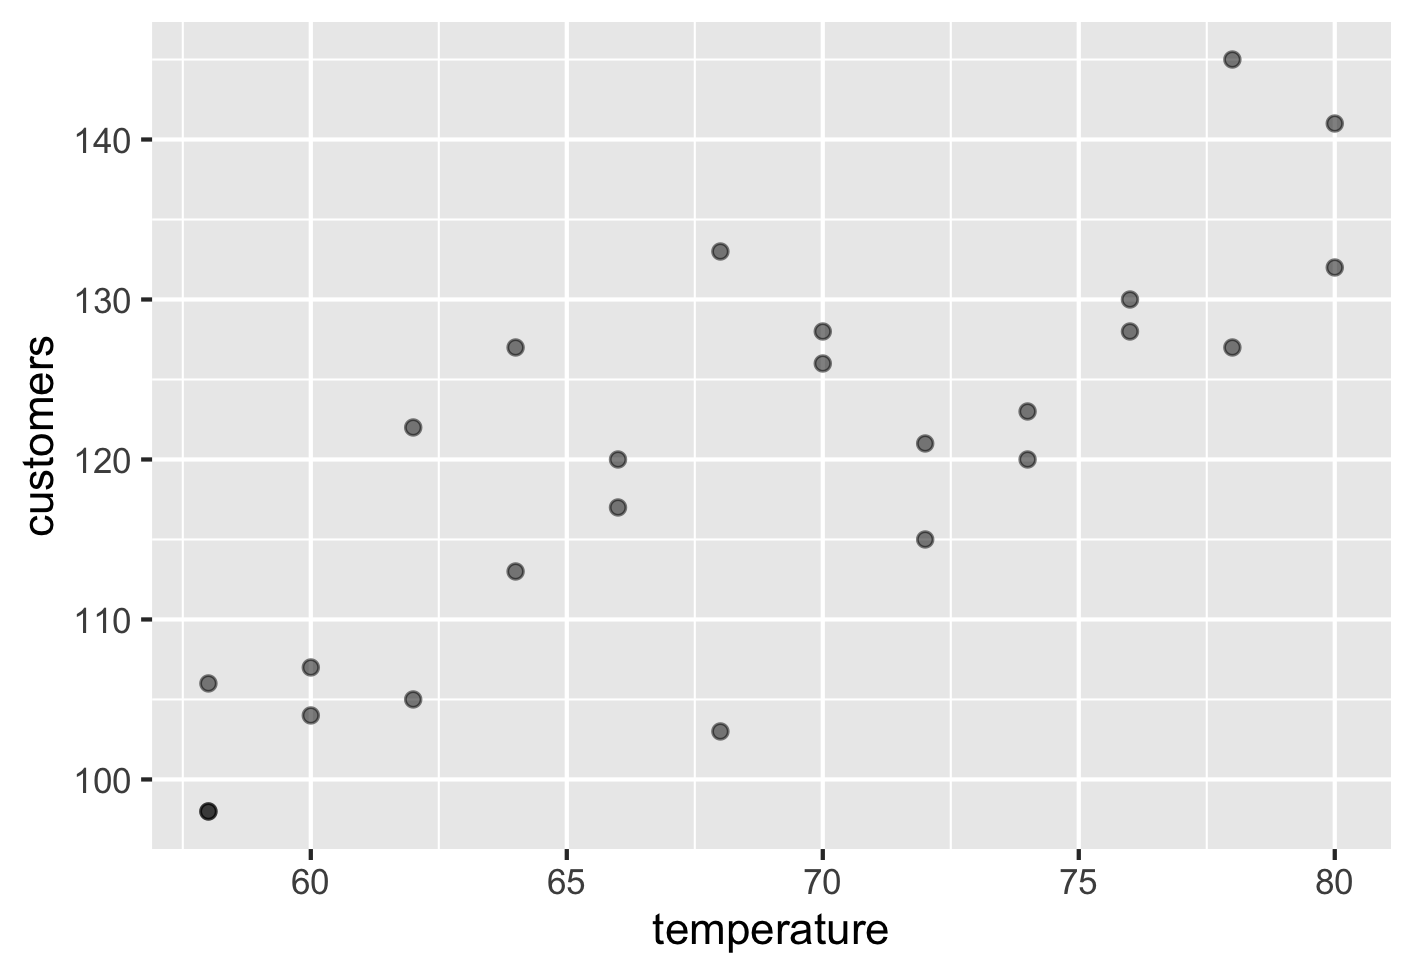
\includegraphics[width=0.7\linewidth,height=\textheight,keepaspectratio]{modules/04-more-on-models/../../images/fig-kiosk-temp-cust-scatter.png}

}

\caption{\label{fig-kiosk-temp-cust-scatter}Scatterplot of
\emph{temperature} against number of \emph{customers} from the
\emph{kiosk} data frame}

\end{figure}%

\begin{tcolorbox}[enhanced jigsaw, colback=white, leftrule=.75mm, toprule=.15mm, bottomtitle=1mm, breakable, coltitle=black, toptitle=1mm, title=\textcolor{quarto-callout-note-color}{\faInfo}\hspace{0.5em}{Quick Check}, opacitybacktitle=0.6, colbacktitle=quarto-callout-note-color!10!white, arc=.35mm, left=2mm, colframe=quarto-callout-note-color-frame, titlerule=0mm, rightrule=.15mm, bottomrule=.15mm, opacityback=0]

Looking at the scatterplot of temperature versus customers
Figure~\ref{fig-kiosk-temp-cust-scatter}:

\begin{itemize}
\tightlist
\item
  Does the relationship appear perfectly linear?
\item
  Does that prevent us from using a linear model?
\end{itemize}

Explain briefly.

\end{tcolorbox}

\begin{tcolorbox}[enhanced jigsaw, colback=white, leftrule=.75mm, toprule=.15mm, bottomtitle=1mm, breakable, coltitle=black, toptitle=1mm, title=\textcolor{quarto-callout-note-color}{\faInfo}\hspace{0.5em}{Answer}, opacitybacktitle=0.6, colbacktitle=quarto-callout-note-color!10!white, arc=.35mm, left=2mm, colframe=quarto-callout-note-color-frame, titlerule=0mm, rightrule=.15mm, bottomrule=.15mm, opacityback=0]

\begin{itemize}
\item
  The relationship is not perfectly linear; there is noticeable scatter
  around what seems to be a somewhat linear pattern.
\item
  This does not prevent us from using a linear model. A linear model is
  a simplification that captures the overall trend, not a claim that all
  points lie exactly on a line.
\end{itemize}

\end{tcolorbox}

Peter then says: ``We have been using
Equation~\ref{eq-kiosk-cust-temp-model-specific} as our tentative model
to explore. In my pre-calculus class, i learned that this is actually
the equation of a straight line. I can add it to the earlier plot.''

He then generates Figure~\ref{fig-kiosk-model-initial-attempt} which has
both the earlier scatterplot and the line from
Equation~\ref{eq-kiosk-cust-temp-model-specific}. (You need not worry
about how he added the line yet. We will learn that shortly.)

\begin{figure}

\centering{

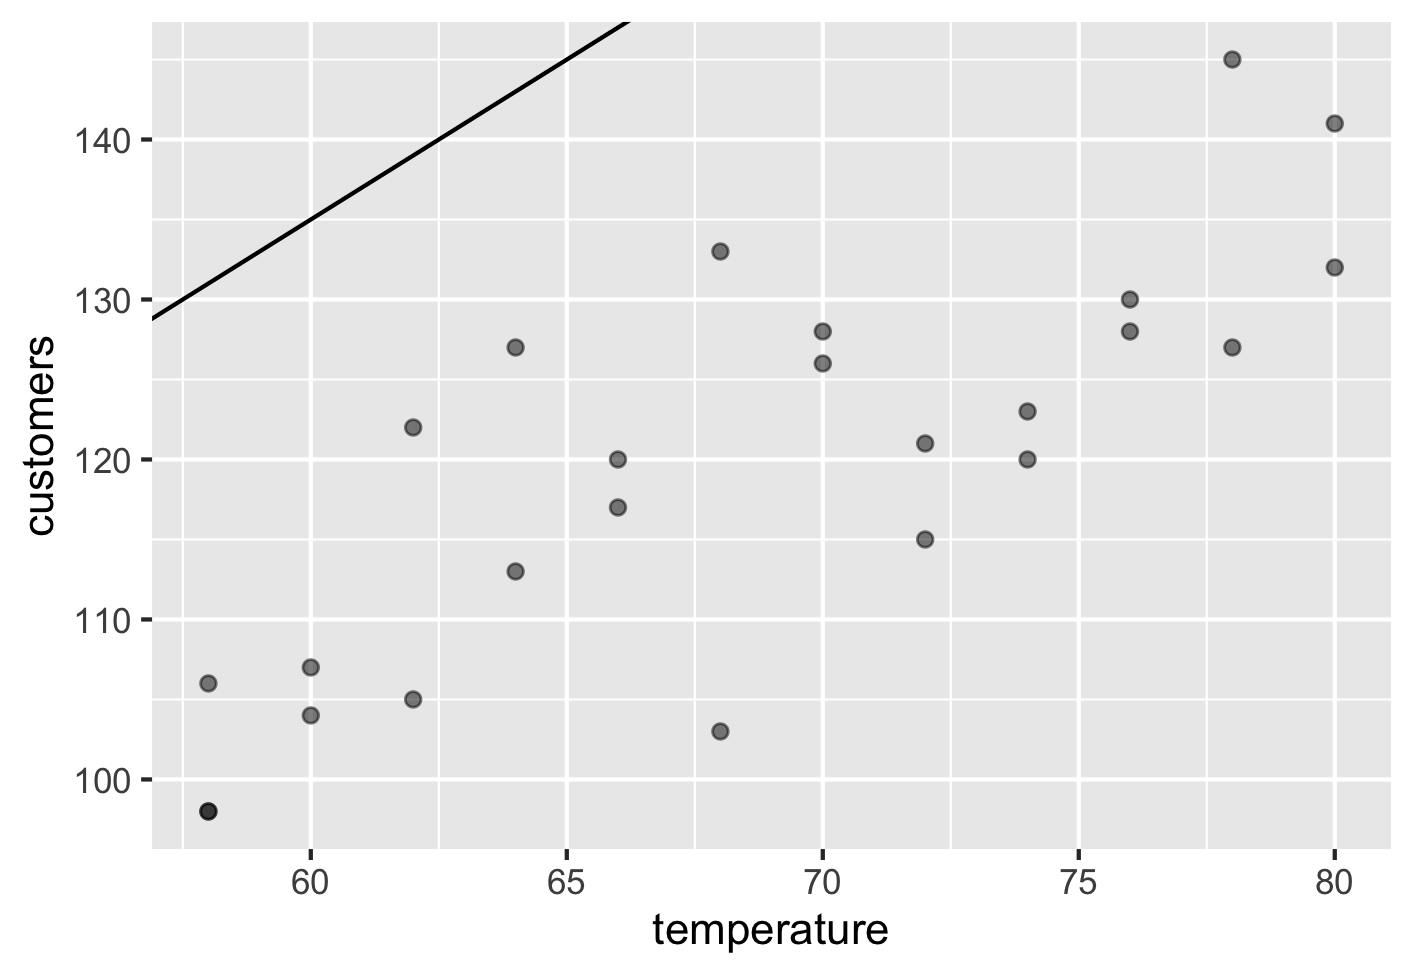
\includegraphics[width=0.7\linewidth,height=\textheight,keepaspectratio]{modules/04-more-on-models/../../images/fig-kiosk-model-initial-attempt.png}

}

\caption{\label{fig-kiosk-model-initial-attempt}Adding a line showing
the kiosk model with \emph{a} = 15 and \emph{b} = 2}

\end{figure}%

Igor says: ``Wow this model is way off the mark! We can reduce the total
penalty by a lot.''

Peter smiles: ``Please explain to us lesser mortals Igor!''

Try to answer by yourself before reading what Igor has to say.

Igor says: ``Well, the line represents the model estimates. If the
estimates are good, they will be near the actual points. But our line
representing the estimate for any temperature is way above the general
region where the points actually lie! For example, we see from
Figure~\ref{fig-kiosk-model-initial-attempt} that two days in our
historical data have had a temperature of 64 degrees. The number of
customers for those two days have been 113 and 127. But the tentative
model from Equation~\ref{eq-kiosk-cust-temp-model-specific} estimates
143. In fact, we can take any actual row of our data and see that the
model estimates are way higher than the general area of the points.
Clearly, we did not make great initial choices for \emph{a} and
\emph{b}! No offense Peter, I know you were just illustrating the form,
and not trying to be exact.''

\begin{tcolorbox}[enhanced jigsaw, colback=white, leftrule=.75mm, toprule=.15mm, bottomtitle=1mm, breakable, coltitle=black, toptitle=1mm, title={Quick Check}, opacitybacktitle=0.6, colbacktitle=quarto-callout-note-color!10!white, arc=.35mm, left=2mm, colframe=quarto-callout-note-color-frame, titlerule=0mm, rightrule=.15mm, bottomrule=.15mm, opacityback=0]

What can we say about the line if we want the model estimates to be
close to the actual values?

\end{tcolorbox}

\begin{tcolorbox}[enhanced jigsaw, colback=white, leftrule=.75mm, toprule=.15mm, bottomtitle=1mm, breakable, coltitle=black, toptitle=1mm, title={Suggested answer}, opacitybacktitle=0.6, colbacktitle=quarto-callout-note-color!10!white, arc=.35mm, left=2mm, colframe=quarto-callout-note-color-frame, titlerule=0mm, rightrule=.15mm, bottomrule=.15mm, opacityback=0]

The line should be right in the middle of the points as far as possible
so that the estimates are close to the actual points.

\end{tcolorbox}

Angela says: ``OK, if we want the model estimates to reflect actual
data, we would want the line to be within the point cloud, and perhaps
generally go through the middle of the cloud. That would make the
estimates at least fall in the general region of the actual values. Let
us try again with different choices for \emph{a} and \emph{b}. How
should we change the values? Should we increase or decrease each one?''

Igor says: ``In Equation~\ref{eq-kiosk-cust-temp-model} \emph{a}
represents where the line intercepts the y-axis at x = 0. I learned this
in my pre-calc class. In that class they called \emph{a} the
\emph{intercept}.''

Suzie jumps up ``But in this plot, the line does not stretch all the way
to the y-axis because we do not have temperature = 0 in our data.''

Igor: ``It does intersect the y-axis, if only we zoom out sufficiently.
Currently the x-axis only starts from around 55.''

Peter quickly modifies the plot to show the origin and lower regions of
the y-axis. Figure~\ref{fig-initial-model-with-intercept-visible} shows
his new plot. This is effectively the same plot as
Figure~\ref{fig-kiosk-model-initial-attempt}, only zoomed out so that we
can see more.

\begin{figure}

\centering{

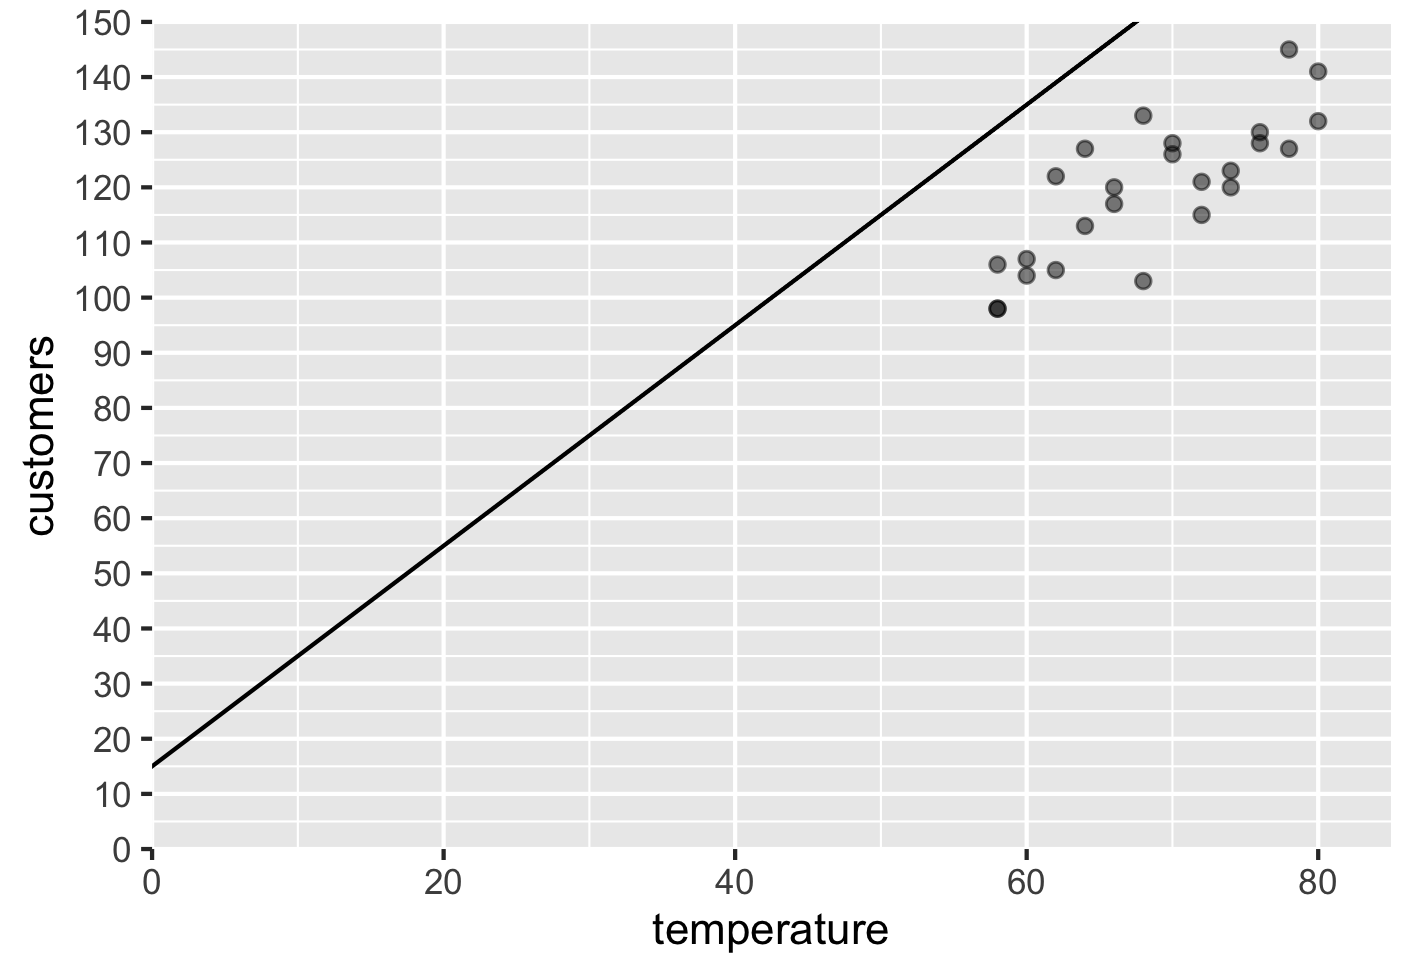
\includegraphics[width=0.7\linewidth,height=\textheight,keepaspectratio]{modules/04-more-on-models/../../images/fig-initial-model-with-intercept-visible.png}

}

\caption{\label{fig-initial-model-with-intercept-visible}Model with
\emph{a} = 15 and \emph{b} = 2 plotted so as to reveal the intercept}

\end{figure}%

\begin{tcolorbox}[enhanced jigsaw, colback=white, leftrule=.75mm, toprule=.15mm, bottomtitle=1mm, breakable, coltitle=black, toptitle=1mm, title=\textcolor{quarto-callout-important-color}{\faExclamation}\hspace{0.5em}{Important}, opacitybacktitle=0.6, colbacktitle=quarto-callout-important-color!10!white, arc=.35mm, left=2mm, colframe=quarto-callout-important-color-frame, titlerule=0mm, rightrule=.15mm, bottomrule=.15mm, opacityback=0]

Even though a temperature of 0°F is well outside our data range,
visualizing the intercept helps us understand what changing \emph{a}
actually does to the line.

\end{tcolorbox}

Suzie: ``From the plot, we can see that the line correctly intersects
the y-axis at 15 since \emph{a = 15}. What can we do to improve the line
so that it goes through the points instead of way above them?''

David opines ``To make the line go through the point cloud, it looks
like we need to make the line less steep, almost like grabbing the top
right of the line and pulling it down. How do we achieve that?''

Peter's pre-calculus comes to the rescue again. ``The value for \emph{b}
determines the steepness of the line or its \emph{slope} also called
\emph{rise over run}. So, we can decrease it to get the line to go
through the cloud of points. Perhaps we should decrease it from 2 to 1.5
and see what happens.''

Peter modifies his plot again. Figure~\ref{fig-kiosk-model-second-guess}
shows his new plot.

\begin{figure}

\centering{

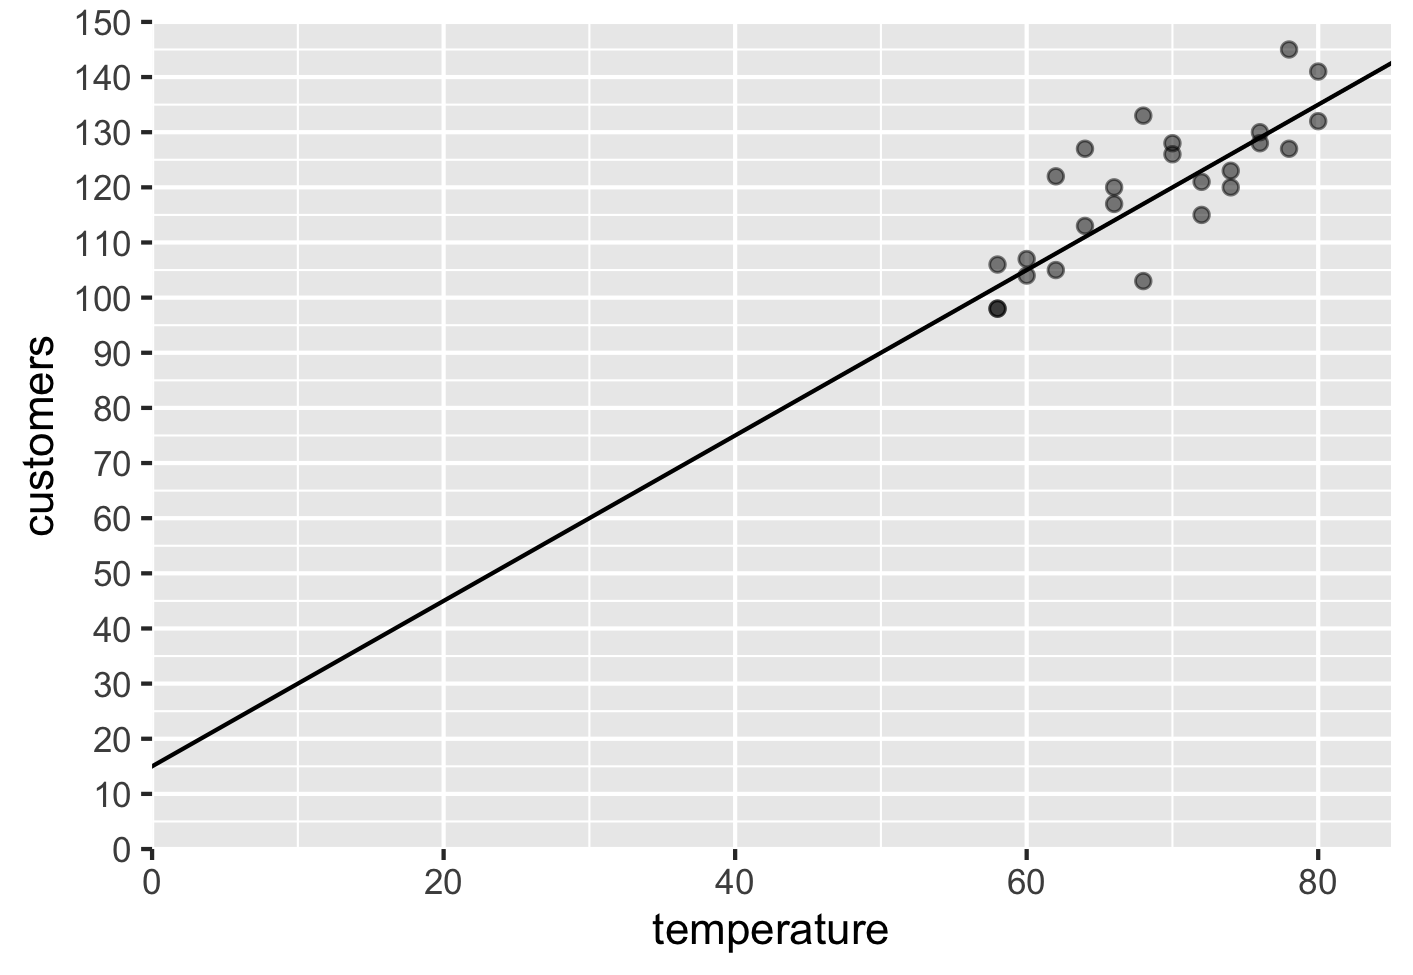
\includegraphics[width=0.7\linewidth,height=\textheight,keepaspectratio]{modules/04-more-on-models/../../images/fig-kiosk-model-second-guess.png}

}

\caption{\label{fig-kiosk-model-second-guess}Second attempt: model with
\emph{a} = 15 and \emph{b} = 1.5}

\end{figure}%

Angela says: ``Wow! that looks so much better! It goes right through the
point cloud. But do we know if it is the \emph{best} line?''

Igor produces the table for this model and announces: ``We have smashed
the total penalty from 28,312 to 1469! But I still don't know if that is
the lowest possible. Maybe there are other values of \emph{a} and
\emph{b} that can reduce it even more.''

Peter, tired of generating more and more plots, says ``We can keep on
trying -- we have an infinite number of choices for \emph{a} and
\emph{b}. How do we find the \emph{best} values for \emph{a} and
\emph{b} that produce the \emph{best line? What does }best* even mean?

\section{\texorpdfstring{What do we mean by the \emph{best}
model?}{What do we mean by the best model?}}\label{what-do-we-mean-by-the-best-model}

In the previous section, the team tried a few values for \emph{a} and
\emph{b} and their second attempt proved to be much better than the
first. However, we want the \emph{best} line. But what does that mean?

David says ``Actually, before visualizing the models, we had already
identified what we mean by \emph{best}. We had already established that
the \emph{best} model or \emph{line}, is the one that generates the
lowest total penalty as we computed in
Table~\ref{tbl-igor-computations-for-15-2}. That is, we choose the
values for \emph{a} and \emph{b} and mimic the process we used for
@btl-igor-computations-for-15-2 and choose the values that produce the
smallest total penalty. But how do we do that when we have an infinite
number of possibilities.''

Angela says: ``Can we not repeat what Suzie did and generate a plot for
various values and visually see what the best values are?''

Peter says: ``Guys, before we think about that, I can help to visualize
the sort of computations we did in
Table~\ref{tbl-igor-computations-for-15-2} but for the line in
Figure~\ref{fig-kiosk-model-second-guess}.'' and comes up with
Figure~\ref{fig-tentative-model-with-residuals-visualized}.

He goes on to explain: ``We are after a model that produces \emph{good}
estimates. Therefore the difference between the actual value and the
model estimate (the column \emph{diff} in
Table~\ref{tbl-igor-computations-for-15-2}) matters. The lower that
difference is, the better.'' He then generates
Figure~\ref{fig-tentative-model-with-residuals-visualized} to visualize
the previous model (\emph{a} = 15 and \emph{b} = 1.5) with the
differences between the actual values and model predictions explicitly
marked for three chosen points. These differences are usually called
\emph{errors} or even better, \emph{residuals}.

\begin{figure}

\centering{

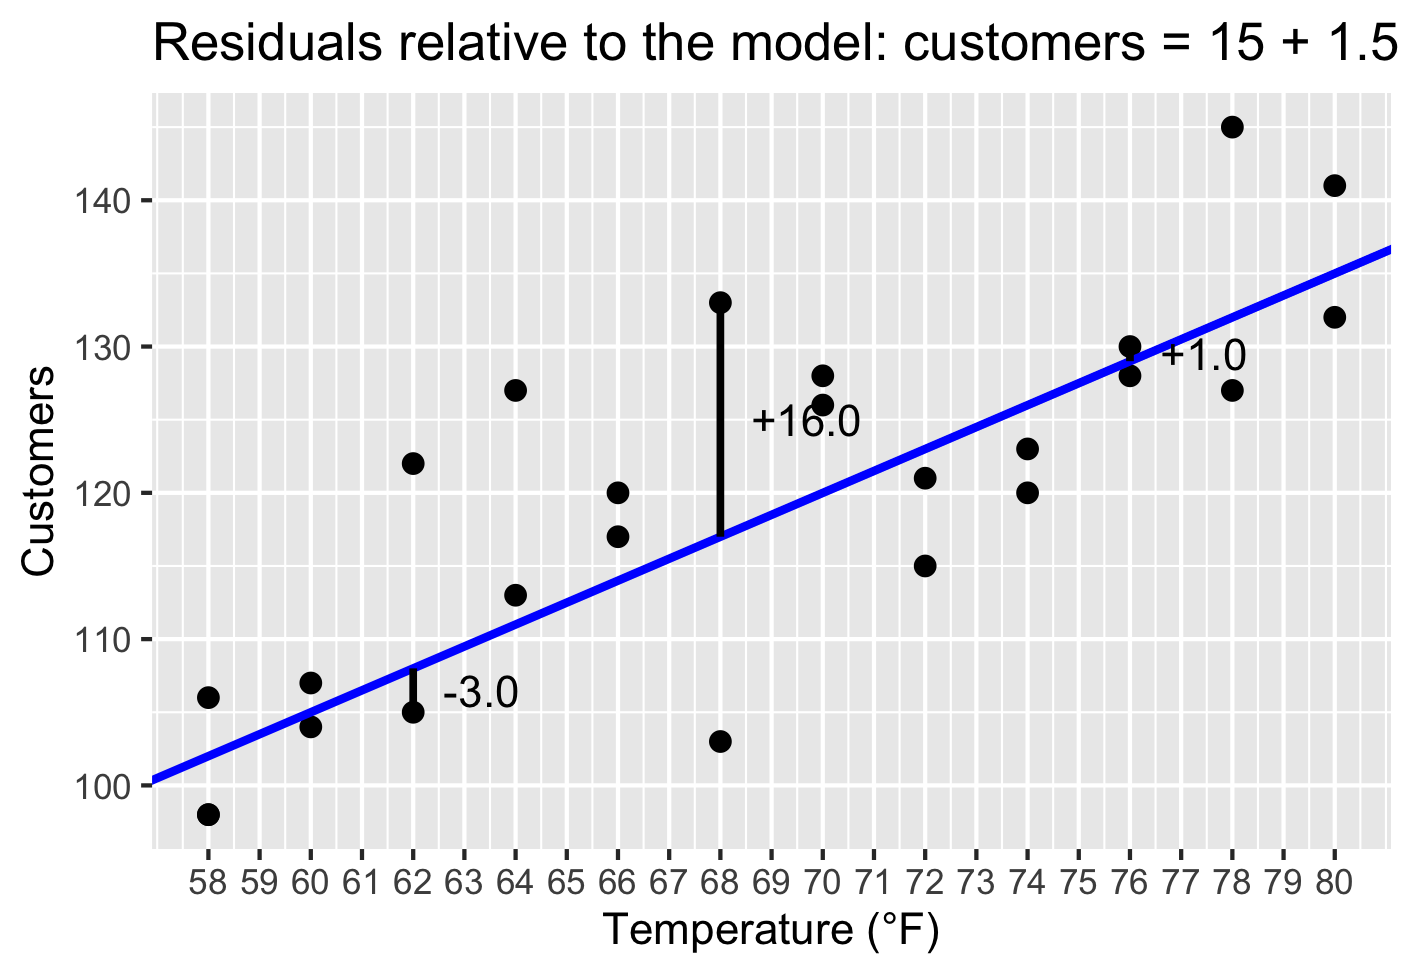
\includegraphics[width=0.7\linewidth,height=\textheight,keepaspectratio]{modules/04-more-on-models/../../images/fig-tentative-model-with-residuals-visualized.png}

}

\caption{\label{fig-tentative-model-with-residuals-visualized}Model with
\emph{a} = 15 and \emph{b} = 1.5 visualized along with the
\emph{residual} or error for three chosen points}

\end{figure}%

\begin{tcolorbox}[enhanced jigsaw, colback=white, leftrule=.75mm, toprule=.15mm, bottomtitle=1mm, breakable, coltitle=black, toptitle=1mm, title=\textcolor{quarto-callout-warning-color}{\faExclamationTriangle}\hspace{0.5em}{Common Misconception}, opacitybacktitle=0.6, colbacktitle=quarto-callout-warning-color!10!white, arc=.35mm, left=2mm, colframe=quarto-callout-warning-color-frame, titlerule=0mm, rightrule=.15mm, bottomrule=.15mm, opacityback=0]

The error or \emph{residual} for an estimate is \textbf{not} the
shortest distance to the line. It is the \textbf{vertical difference}
between the observed value and the estimated value. This is because our
model estimates the response (customers) and we compare that to the
actual number of customers for any point.

\end{tcolorbox}

David points to
Figure~\ref{fig-tentative-model-with-residuals-visualized} and says:
``For the point at \emph{temperature = 62}, the actual data had
\emph{customers = 105}, whereas our model estimates 108. So the model is
off by -3 (if we compute the residual using this equation.'' and he
writes out Equation~\ref{eq-residual-1}.

\begin{equation}\phantomsection\label{eq-residual-1}{
\text{residual} = \text{actual value} - \text{model estimate}
}\end{equation}

Peter continues: ``For the data point with \emph{temperature = 68}, the
model estimates 116, whereas the actual value was 132 for a residual of
+16. Finally, for the point where the \emph{temperature} is 76, the
model estimates 129, whereas the actual value was 130. The model did
well on this point. In this way, we can compute the \emph{residual} for
every point and square it. We are not particularly concerned about the
actual sign of the residual since we are going to square it anyway. This
is exactly what Igor showed us in
Table~\ref{tbl-igor-computations-for-15-2}.''

\begin{tcolorbox}[enhanced jigsaw, colback=white, leftrule=.75mm, toprule=.15mm, bottomtitle=1mm, breakable, coltitle=black, toptitle=1mm, title=\textcolor{quarto-callout-note-color}{\faInfo}\hspace{0.5em}{Quick Check}, opacitybacktitle=0.6, colbacktitle=quarto-callout-note-color!10!white, arc=.35mm, left=2mm, colframe=quarto-callout-note-color-frame, titlerule=0mm, rightrule=.15mm, bottomrule=.15mm, opacityback=0]

If a model estimates 120 customers for a given temperature, and the
actual number is 132:

\begin{itemize}
\tightlist
\item
  What is the residual or error in this estimate?
\item
  Is it positive or negative?
\end{itemize}

\end{tcolorbox}

\begin{tcolorbox}[enhanced jigsaw, colback=white, leftrule=.75mm, toprule=.15mm, bottomtitle=1mm, breakable, coltitle=black, toptitle=1mm, title=\textcolor{quarto-callout-note-color}{\faInfo}\hspace{0.5em}{Answer}, opacitybacktitle=0.6, colbacktitle=quarto-callout-note-color!10!white, arc=.35mm, left=2mm, colframe=quarto-callout-note-color-frame, titlerule=0mm, rightrule=.15mm, bottomrule=.15mm, opacityback=0]

The estimate's error is 132 − 120 = 12.

The error is positive because the actual value is higher than the
estimated value.

\end{tcolorbox}

Angela says: ``If we draw any line through these points, each line will
have low \emph{absolute residuals} for some points and higher ones for
others. But we have many points and so we want an \emph{overall measure
of how close the line is to }all the points* by considering all the
\emph{residuals}. Even if a line is spot-on for a few points, it is not
very useful if it is wildly off for many others. That overall measure is
in fact the total penalty from
Table~\ref{tbl-igor-computations-for-15-2}. It is very nice that we have
seen the computations and also seen its visualization to make sure we
understand all this. I sure am glad we are doing this as a team!''

Igor says, ``Yes, now I too see the connection between my table
(Table~\ref{tbl-igor-computations-for-15-2}) and Peter's visualization
of the concept. So, we will square the residuals from all the points and
add them all up. That is how much total penalty the line/model has when
we consider \emph{all} data points. As Amanda wanted, squaring punishes
bigger residuals much more than smaller ones. I have heard that this is
a standard theme in statistics.''

\begin{tcolorbox}[enhanced jigsaw, colback=white, leftrule=.75mm, toprule=.15mm, bottomtitle=1mm, breakable, coltitle=black, toptitle=1mm, title=\textcolor{quarto-callout-important-color}{\faExclamation}\hspace{0.5em}{What's the deal with squaring?}, opacitybacktitle=0.6, colbacktitle=quarto-callout-important-color!10!white, arc=.35mm, left=2mm, colframe=quarto-callout-important-color-frame, titlerule=0mm, rightrule=.15mm, bottomrule=.15mm, opacityback=0]

We square errors for the same reason we used squared deviations when
defining variance:

\begin{itemize}
\tightlist
\item
  positive and negative errors should not cancel out
\item
  larger errors should count more than smaller ones
\end{itemize}

Least squares regression that we study in this course is built on the
same logic as variance. In a later chapter, we will see this idea pop
when we look at the explanatory power of a model. Hang tight till then!

\end{tcolorbox}

\begin{tcolorbox}[enhanced jigsaw, colback=white, leftrule=.75mm, toprule=.15mm, bottomtitle=1mm, breakable, coltitle=black, toptitle=1mm, title=\textcolor{quarto-callout-note-color}{\faInfo}\hspace{0.5em}{Quick Check}, opacitybacktitle=0.6, colbacktitle=quarto-callout-note-color!10!white, arc=.35mm, left=2mm, colframe=quarto-callout-note-color-frame, titlerule=0mm, rightrule=.15mm, bottomrule=.15mm, opacityback=0]

Why don't we choose the line that minimizes the \textbf{sum of errors}
instead of the \textbf{sum of squared errors}?

\end{tcolorbox}

\begin{tcolorbox}[enhanced jigsaw, colback=white, leftrule=.75mm, toprule=.15mm, bottomtitle=1mm, breakable, coltitle=black, toptitle=1mm, title=\textcolor{quarto-callout-note-color}{\faInfo}\hspace{0.5em}{Answer}, opacitybacktitle=0.6, colbacktitle=quarto-callout-note-color!10!white, arc=.35mm, left=2mm, colframe=quarto-callout-note-color-frame, titlerule=0mm, rightrule=.15mm, bottomrule=.15mm, opacityback=0]

Positive and negative errors would cancel out if we summed errors
directly.

Squaring errors ensures that all errors contribute positively and that
larger errors are penalized more heavily.

There is a kind of model that works b y minimizing absolute errors too,
but we do not look at that in this course.

\end{tcolorbox}

\begin{tcolorbox}[enhanced jigsaw, colback=white, leftrule=.75mm, toprule=.15mm, bottomtitle=1mm, breakable, coltitle=black, toptitle=1mm, title={Quick Check}, opacitybacktitle=0.6, colbacktitle=quarto-callout-note-color!10!white, arc=.35mm, left=2mm, colframe=quarto-callout-note-color-frame, titlerule=0mm, rightrule=.15mm, bottomrule=.15mm, opacityback=0]

In what sense is the line in
Figure~\ref{fig-tentative-model-with-residuals-visualized} better than
the one in Figure~\ref{fig-initial-model-with-intercept-visible}?

\end{tcolorbox}

\begin{tcolorbox}[enhanced jigsaw, colback=white, leftrule=.75mm, toprule=.15mm, bottomtitle=1mm, breakable, coltitle=black, toptitle=1mm, title={Suggested answer}, opacitybacktitle=0.6, colbacktitle=quarto-callout-note-color!10!white, arc=.35mm, left=2mm, colframe=quarto-callout-note-color-frame, titlerule=0mm, rightrule=.15mm, bottomrule=.15mm, opacityback=0]

The line in Figure~\ref{fig-tentative-model-with-residuals-visualized}
is much closer to each of the points than the one in
Figure~\ref{fig-initial-model-with-intercept-visible}. Consequently it
will have much lower residuals for almost any point.

\end{tcolorbox}

David says: ``For this model (a = 15, b = 1.5), the total of all the
squared residuals is: 1,469. Is there a line that can give an even lower
value? What are the values for \emph{a} and \emph{b} for which we get
the \emph{lowest} possible total of all the squared residuals?''

The team now understands exactly what they mean by the \emph{best}
model. They are looking for values for \emph{a} and \emph{b} that will
result in the lowest total penalty. But they are stuck on to how to
actually get it.

Returning to the idea of trying to generate a plot to identify the best
values just like Suzie did in the first week, Angela asks ``Suzie, can
you do you pull off your plotting magic again, please?''

Suzie: ``Well angela, that would be a three-dimensional plot because we
will have \emph{a}, \emph{b}, and the \emph{total penalty} all on the
same plot. I can do it, but I am afraid it will not be much help.''

Igor: ``Wht not just print out a large table of all combinations of
\emph{a} and \emph{b} and the total penalty for each combination? We can
then look through the table and select the best value -- or even ask the
program to look through the table and find the values for us?''

Suzie says ``We can Igor, but I have two issues. Firstly, when I try the
various combinations of \emph{a} and \emph{b}, I can only do it in some
intervals like 0.1 or something like that. What if the best solution was
between two of my values? We will then not get an exact solution, but we
will get something very close. A bigger problem is what if Amanda comes
up with two more variables to use in our predictions? Then trying all
combinations can generate a very large number of rows, perhaps millions.
There has to be a better way.''

Steve, who has been silent for a long time has actually been having a
nagging feeling that he has done something similar in one of his
classes. He now says ``I think we learned something like this in my econ
class. Rather than making Suzie write a whole new program, I think there
is a function in R, based in calculus, that can readily do this for us!
Let me try.''

And he runs the code below: which generates the \emph{best} values for
\emph{a} and \emph{b} that guarantee that the \emph{sum of squared
residuals} is the smallest possible.

\begin{lstlisting}[language=R]
kiosk |> 
  model_train(customers ~ temperature) |> 
  coef()
\end{lstlisting}

\begin{lstlisting}
(Intercept) temperature 
      22.06        1.42 
\end{lstlisting}

Steve then explains: ``Ah, now I remember what the output means. We see
two values in the output: \emph{intercept} and \emph{temperature}. The
first is \emph{a} and the second is \emph{b}! These are exactly the
values of \emph{a} and \emph{b} that minimize the sum of squared
residuals. These are the values that give us the \emph{best} possible
line!''

From the output, Steve then writes the model equation
Equation~\ref{eq-kiosk-cust-temp-model-best}, and says:

``This equation shows the \emph{best model} for our problem, given that
we want a straight line and want to minimize the sum of squared
residuals.''

``Our econ teacher called this the least-squares regression line.''

\begin{equation}\phantomsection\label{eq-kiosk-cust-temp-model-best}{
\widehat{\text{customers}} = 22.06 +  1.42\times\text{temperature}
}\end{equation}

\begin{tcolorbox}[enhanced jigsaw, colback=white, leftrule=.75mm, toprule=.15mm, bottomtitle=1mm, breakable, coltitle=black, toptitle=1mm, title=\textcolor{quarto-callout-note-color}{\faInfo}\hspace{0.5em}{Key Idea}, opacitybacktitle=0.6, colbacktitle=quarto-callout-note-color!10!white, arc=.35mm, left=2mm, colframe=quarto-callout-note-color-frame, titlerule=0mm, rightrule=.15mm, bottomrule=.15mm, opacityback=0]

Since there is an infinite number of possible choices for \emph{a} and
\emph{b}, we need a systematic way to find the values that minimize the
total of the squared residuals. Mathematically, this problem can be
solved using calculus. Practically, we sit back and let software do this
for us.

\end{tcolorbox}

\begin{tcolorbox}[enhanced jigsaw, colback=white, leftrule=.75mm, toprule=.15mm, bottomtitle=1mm, breakable, coltitle=black, toptitle=1mm, title=\textcolor{quarto-callout-note-color}{\faInfo}\hspace{0.5em}{Pause \& Think}, opacitybacktitle=0.6, colbacktitle=quarto-callout-note-color!10!white, arc=.35mm, left=2mm, colframe=quarto-callout-note-color-frame, titlerule=0mm, rightrule=.15mm, bottomrule=.15mm, opacityback=0]

Complete the sentence:

``A least squares regression line is the line that \_\_\_\_\_.''

\end{tcolorbox}

\begin{tcolorbox}[enhanced jigsaw, colback=white, leftrule=.75mm, toprule=.15mm, bottomtitle=1mm, breakable, coltitle=black, toptitle=1mm, title=\textcolor{quarto-callout-note-color}{\faInfo}\hspace{0.5em}{Answer}, opacitybacktitle=0.6, colbacktitle=quarto-callout-note-color!10!white, arc=.35mm, left=2mm, colframe=quarto-callout-note-color-frame, titlerule=0mm, rightrule=.15mm, bottomrule=.15mm, opacityback=0]

A least squares regression line is the line that minimizes the sum of
squared vertical estimation errors, or the sum of squared residuals
(same thing).

\end{tcolorbox}

Igor is at it again. He announces ``The total penalty for this is 1388.
This beats the 1469 we got earlier. And, according to Steve, this is the
\emph{best}. I am quite impressed that we had eyeballed a solution this
close to the best!''

\begin{tcolorbox}[enhanced jigsaw, colback=white, leftrule=.75mm, toprule=.15mm, bottomtitle=1mm, breakable, coltitle=black, toptitle=1mm, title=\textcolor{quarto-callout-important-color}{\faExclamation}\hspace{0.5em}{Important}, opacitybacktitle=0.6, colbacktitle=quarto-callout-important-color!10!white, arc=.35mm, left=2mm, colframe=quarto-callout-important-color-frame, titlerule=0mm, rightrule=.15mm, bottomrule=.15mm, opacityback=0]

The team found a line that \emph{minimizes the sum of squared
residuals}. Technically this is called the \emph{least-squares
criterion} and plays a very important role in statistics and data
analysis.

\end{tcolorbox}

They explain the model to Amanda. After a lot of questioning to
understand their decision criteria, Amanda agrees to use this model for
the next month.

Amanda seems thrilled with their work. ``Great work team. Talk to me
when you graduate. I want to assemble a business analytics team for my
businesses and I sure can do with a team like yours.''

\begin{tcolorbox}[enhanced jigsaw, colback=white, leftrule=.75mm, toprule=.15mm, bottomtitle=1mm, breakable, coltitle=black, toptitle=1mm, title=\textcolor{quarto-callout-note-color}{\faInfo}\hspace{0.5em}{Pause \& Think}, opacitybacktitle=0.6, colbacktitle=quarto-callout-note-color!10!white, arc=.35mm, left=2mm, colframe=quarto-callout-note-color-frame, titlerule=0mm, rightrule=.15mm, bottomrule=.15mm, opacityback=0]

Suppose tomorrow's high temperature is 73°F. Your model estimates 124
customers.

\begin{itemize}
\tightlist
\item
  Does this mean exactly 124 customers will arrive?
\item
  What other factors (besides temperature) might cause the actual number
  to be higher or lower?
\end{itemize}

What does this tell you about what a regression model can, and cannot,
do?

\end{tcolorbox}

\begin{tcolorbox}[enhanced jigsaw, colback=white, leftrule=.75mm, toprule=.15mm, bottomtitle=1mm, breakable, coltitle=black, toptitle=1mm, title={Suggested answer}, opacitybacktitle=0.6, colbacktitle=quarto-callout-note-color!10!white, arc=.35mm, left=2mm, colframe=quarto-callout-note-color-frame, titlerule=0mm, rightrule=.15mm, bottomrule=.15mm, opacityback=0]

\begin{itemize}
\item
  No.~124 is only a model estimation. In reality the number of customers
  may be 124 or higher or lower.
\item
  The model acts as if only the temperature determines the number of
  customers. In reality, many other factors play a role too. Perhaps
  there is a football game in town and that draws people away. Perhaps
  the humidity is unusually high and people stay away. Many factors play
  a role in this. Our model uses a simple rule that can potentially
  perform decently without being accurate and overly complex.
\end{itemize}

In later chapters we will see that we can include more variables in a
model and improve its performance.

\end{tcolorbox}

\section{Optional enrichment topic: Beyond straight
lines}\label{optional-enrichment-topic-beyond-straight-lines}

In this chapter, we have assumed that a straight line is a reasonable
model for the relationship between temperature and customer traffic. In
many business settings, this assumption works well: simple models are
easy to interpret, easy to communicate, and often good enough for
decision-making.

However, not all relationships are well captured by a straight line.

\subsection{When a straight line may not be
appropriate}\label{when-a-straight-line-may-not-be-appropriate}

In some situations, a scatterplot may reveal patterns such as:

\begin{itemize}
\item
  curvature (the relationship bends),
\item
  diminishing returns (the effect of increases slows down), or
\item
  threshold effects (behavior changes after a certain point).
\end{itemize}

For example, at very high temperatures, customer traffic at a beach
kiosk might level off or even decline as conditions become
uncomfortable. A straight line cannot capture this kind of behavior
well, no matter how its slope and intercept are chosen.

In such cases, forcing a linear model may lead to systematic residual
patterns, indicating that the model is missing something important.

\subsection{A flexible alternative: LOWESS
smoothing}\label{a-flexible-alternative-lowess-smoothing}

One way to explore nonlinear relationships is through a technique called
LOWESS (short for locally weighted scatterplot smoothing).

Figure~\ref{fig-lowess-example} shows an example of a LOWESS model using
the \emph{mpg} data frame. In this data frame the \emph{displacement} of
an engine is related to the highway mileage \emph{hwy}, but not in a
linear way. The LOWESS model better describes it than a straight line
would. Like the earlier line model, this too can take in a value for
\emph{displ} and provide an estimated value for \emph{hwy}.

\begin{figure}

\centering{

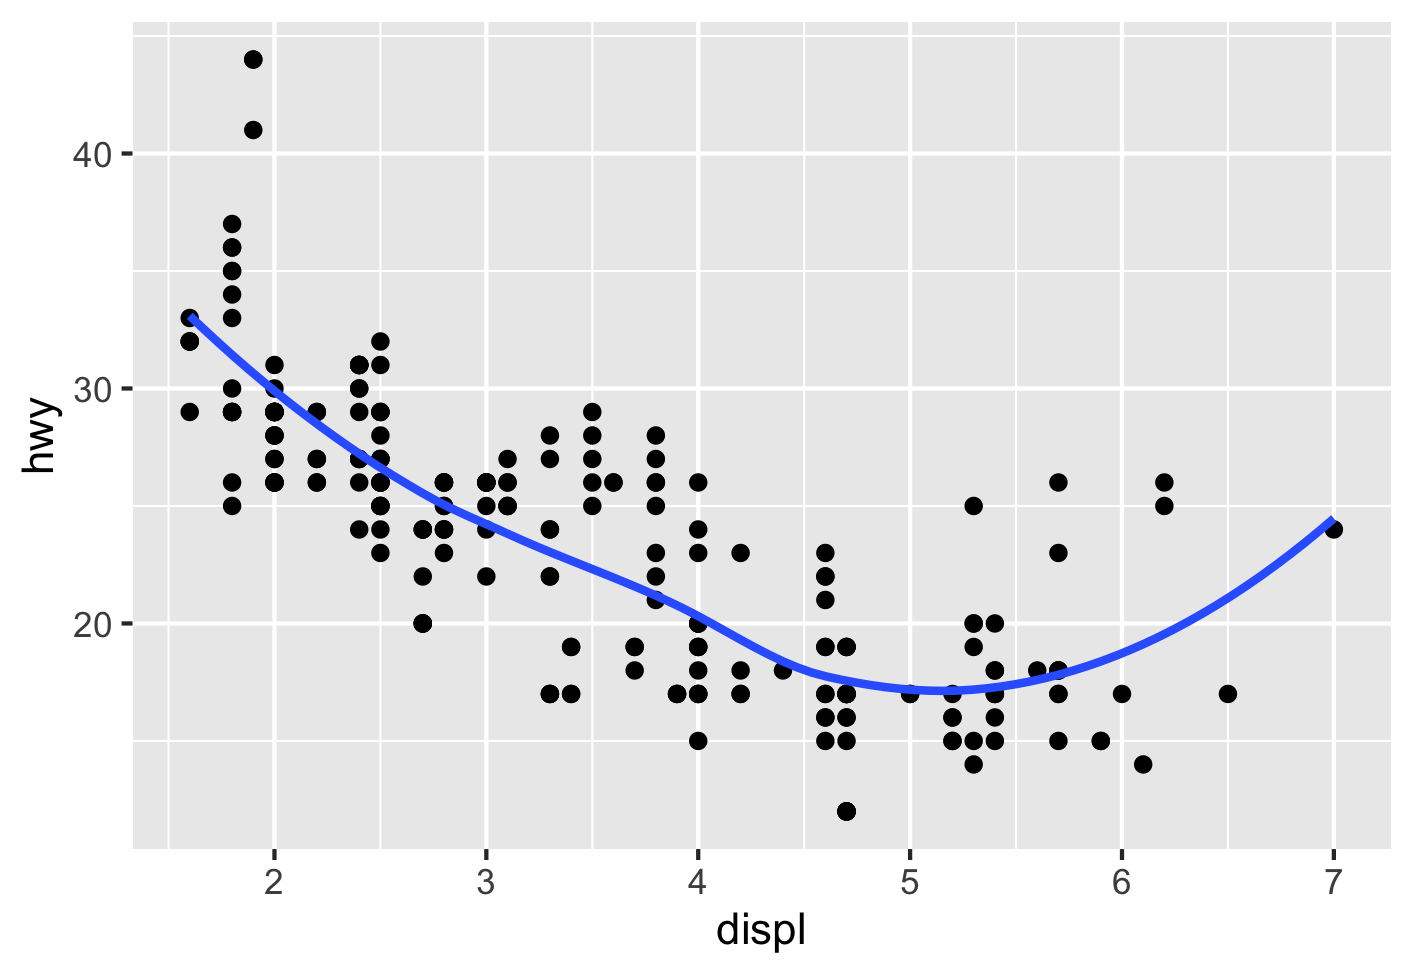
\includegraphics[width=0.7\linewidth,height=\textheight,keepaspectratio]{modules/04-more-on-models/../../images/fig-lowess-example.png}

}

\caption{\label{fig-lowess-example}LOWESS model for \emph{displacement}
vs \emph{cty} in the \emph{mpg} data frame showing how it captures the
curvature in the relationship better than a lien can}

\end{figure}%

Rather than fitting a single global rule like a straight line, LOWESS
works by:

\begin{itemize}
\item
  focusing on a small neighborhood of points around each value of the
  explanatory variable, and
\item
  fitting simple local models that adapt to the data in that
  neighborhood.
\end{itemize}

The result is a smooth curve that follows the overall pattern of the
data without requiring us to specify a particular functional form in
advance.

LOWESS is especially useful for:

\begin{itemize}
\item
  exploratory analysis,
\item
  visualizing trends, and
\item
  diagnosing whether a straight-line model is reasonable.
\end{itemize}

It is not intended to replace regression models in all cases, but rather
to help us understand the structure of the data.

\subsection{Models as choices, not
defaults}\label{models-as-choices-not-defaults}

The key takeaway is not that linear models are ``wrong,'' but that
models are choices.

\begin{itemize}
\item
  A straight line is a good choice when the relationship is
  approximately linear and interpretability matters.
\item
  A nonlinear model may be a better choice when the data clearly suggest
  curvature or changing behavior.
\item
  Flexible tools like LOWESS help us see what the data are trying to
  tell us before we commit to a specific model.
\end{itemize}

In all cases, the central modeling question remains the same:

\begin{quote}
Does this model capture the important structure in the data well enough
to support the decisions we want to make?
\end{quote}

This mindset---treating models as purposeful approximations rather than
automatic formulas---will guide us throughout the rest of this book.

\chapter{Visualizing Models}\label{sec-visualizing-models}

In this chapter, we will first revisit how to build visualize the two
\emph{mean} models we saw earlier in Chapter~\ref{sec-mean-model} and
Chapter~\ref{sec-category-means}. To be sure, we already covered these
in Chapter~\ref{sec-visualizing-mean-models}, but repeat it with
different examples to provide reinforcement.

We will then learn how to visualize line models that we learned about in
Chapter~\ref{sec-best-fit-line}. This will set the stage for us to learn
how to \emph{build} these models and construct the models as equations.

\section{Recap of models}\label{recap-of-models}

From prior chapters, we have learned that a model takes as input the
values of the explanatory variable(s) (if any) and outputs an estimated
value of the outcome variable.

We started off in Chapter~\ref{sec-mean-model} by showing that, in the
absence of an explanatory variable, the \emph{mean} is the best model.
For example, our \emph{mpg} data frame contains data about several cars.
Let us suppose that our outcome variable is \emph{hwy}, the highway
mileage of a car.

If we are given only the data from that single column \emph{hwy}, and
nothing else, the best \emph{model} we can come up with for
\emph{estimating} the highway mileage of a car is to always provide the
average highway mileage from the data set.

We then considered, in Chapter~\ref{sec-category-means}, the case where
we had a single explanatory variable, a categorical one and saw that
here too the same idea applies, except that the best model for a
category is the average for that category.

We then studied, in Chapter~\ref{sec-best-fit-line} the case of a single
explanatory variable again, but this time the explanatory variable was
numerical. We learned there about the \emph{least squares criterion} to
find the best model.

Chapter~\ref{sec-visualizing-mean-models} showed us how to visualize the
models we built around the idea of the \emph{mean} as a model in
Chapter~\ref{sec-mean-model} and @\#sec-category-means. In this chapter,
we use new examples to briefly review how to visualize those models and
also compute and write out the model functions. We then move on to
visualizing our line models from Chapter~\ref{sec-best-fit-line} and how
to build and reconstruct the model function as an equation.

We will first learn how to visualize the models. We then look at how to
generate the model function in equation form.

\section{Visualizing simple mean models (no explanatory
variable)}\label{visualizing-simple-mean-models-no-explanatory-variable}

We take a different dataset this time. The data frame \emph{txhousing}
contains real estate data for the state of Texas for several years. We
first follow the good practice of understanding the dataset before
jumping in and building models. Table~\ref{tbl-txhousing-head-10} shows
the first 10 rows .

\begin{lstlisting}[language=R]
txhousing |>
    head(10) 
\end{lstlisting}

\begin{longtable}[]{@{}
  >{\raggedright\arraybackslash}p{(\linewidth - 16\tabcolsep) * \real{0.1231}}
  >{\raggedleft\arraybackslash}p{(\linewidth - 16\tabcolsep) * \real{0.0769}}
  >{\raggedleft\arraybackslash}p{(\linewidth - 16\tabcolsep) * \real{0.0923}}
  >{\raggedleft\arraybackslash}p{(\linewidth - 16\tabcolsep) * \real{0.0923}}
  >{\raggedleft\arraybackslash}p{(\linewidth - 16\tabcolsep) * \real{0.1385}}
  >{\raggedleft\arraybackslash}p{(\linewidth - 16\tabcolsep) * \real{0.1077}}
  >{\raggedleft\arraybackslash}p{(\linewidth - 16\tabcolsep) * \real{0.1385}}
  >{\raggedleft\arraybackslash}p{(\linewidth - 16\tabcolsep) * \real{0.1538}}
  >{\raggedleft\arraybackslash}p{(\linewidth - 16\tabcolsep) * \real{0.0769}}@{}}
\caption{First 10 rows from the \emph{txhousing} data
frame}\label{tbl-txhousing-head-10}\tabularnewline
\toprule\noalign{}
\begin{minipage}[b]{\linewidth}\raggedright
city
\end{minipage} & \begin{minipage}[b]{\linewidth}\raggedleft
year
\end{minipage} & \begin{minipage}[b]{\linewidth}\raggedleft
month
\end{minipage} & \begin{minipage}[b]{\linewidth}\raggedleft
sales
\end{minipage} & \begin{minipage}[b]{\linewidth}\raggedleft
volume
\end{minipage} & \begin{minipage}[b]{\linewidth}\raggedleft
median
\end{minipage} & \begin{minipage}[b]{\linewidth}\raggedleft
listings
\end{minipage} & \begin{minipage}[b]{\linewidth}\raggedleft
inventory
\end{minipage} & \begin{minipage}[b]{\linewidth}\raggedleft
date
\end{minipage} \\
\midrule\noalign{}
\endfirsthead
\toprule\noalign{}
\begin{minipage}[b]{\linewidth}\raggedright
city
\end{minipage} & \begin{minipage}[b]{\linewidth}\raggedleft
year
\end{minipage} & \begin{minipage}[b]{\linewidth}\raggedleft
month
\end{minipage} & \begin{minipage}[b]{\linewidth}\raggedleft
sales
\end{minipage} & \begin{minipage}[b]{\linewidth}\raggedleft
volume
\end{minipage} & \begin{minipage}[b]{\linewidth}\raggedleft
median
\end{minipage} & \begin{minipage}[b]{\linewidth}\raggedleft
listings
\end{minipage} & \begin{minipage}[b]{\linewidth}\raggedleft
inventory
\end{minipage} & \begin{minipage}[b]{\linewidth}\raggedleft
date
\end{minipage} \\
\midrule\noalign{}
\endhead
\bottomrule\noalign{}
\endlastfoot
Abilene & 2000 & 1 & 72 & 5380000 & 71400 & 701 & 6.3 & 2000 \\
Abilene & 2000 & 2 & 98 & 6505000 & 58700 & 746 & 6.6 & 2000 \\
Abilene & 2000 & 3 & 130 & 9285000 & 58100 & 784 & 6.8 & 2000 \\
Abilene & 2000 & 4 & 98 & 9730000 & 68600 & 785 & 6.9 & 2000 \\
Abilene & 2000 & 5 & 141 & 10590000 & 67300 & 794 & 6.8 & 2000 \\
Abilene & 2000 & 6 & 156 & 13910000 & 66900 & 780 & 6.6 & 2000 \\
Abilene & 2000 & 7 & 152 & 12635000 & 73500 & 742 & 6.2 & 2000 \\
Abilene & 2000 & 8 & 131 & 10710000 & 75000 & 765 & 6.4 & 2001 \\
Abilene & 2000 & 9 & 104 & 7615000 & 64500 & 771 & 6.5 & 2001 \\
Abilene & 2000 & 10 & 101 & 7040000 & 59300 & 764 & 6.6 & 2001 \\
\end{longtable}

We see that for the first 10 rows, \emph{city} and \emph{year} are the
same, but there is variation in the other variables. The dataset has
8602 observations or rows. Use the command ?txhousing in RStudio to
answer the following questions.

\begin{tcolorbox}[enhanced jigsaw, colback=white, leftrule=.75mm, toprule=.15mm, bottomtitle=1mm, breakable, coltitle=black, toptitle=1mm, title={Quick Check}, opacitybacktitle=0.6, colbacktitle=quarto-callout-note-color!10!white, arc=.35mm, left=2mm, colframe=quarto-callout-note-color-frame, titlerule=0mm, rightrule=.15mm, bottomrule=.15mm, opacityback=0]

What is the \emph{unit of observation} int his dataset? Unfortunately,
the codebook does not give sufficient details. Se if you can use ChatGPT
or other chatbot to find the answer.

\end{tcolorbox}

\begin{tcolorbox}[enhanced jigsaw, colback=white, leftrule=.75mm, toprule=.15mm, bottomtitle=1mm, breakable, coltitle=black, toptitle=1mm, title={Suggested answer}, opacitybacktitle=0.6, colbacktitle=quarto-callout-note-color!10!white, arc=.35mm, left=2mm, colframe=quarto-callout-note-color-frame, titlerule=0mm, rightrule=.15mm, bottomrule=.15mm, opacityback=0]

For every city in Texas, the dataset has its real estate activity for
one month. The data spans 12 months each from 2000 to 2014 and for 2015
7 months from Jan to July. There are 46 cities. For each city we have
data for 180 + 7 = 187 months. Therefore the unit of observation is the
real estate activity for a single city for a single month.

\end{tcolorbox}

\begin{tcolorbox}[enhanced jigsaw, colback=white, leftrule=.75mm, toprule=.15mm, bottomtitle=1mm, breakable, coltitle=black, toptitle=1mm, title={Quick Check}, opacitybacktitle=0.6, colbacktitle=quarto-callout-note-color!10!white, arc=.35mm, left=2mm, colframe=quarto-callout-note-color-frame, titlerule=0mm, rightrule=.15mm, bottomrule=.15mm, opacityback=0]

Explain precisely what the first row tells us.

\end{tcolorbox}

\begin{tcolorbox}[enhanced jigsaw, colback=white, leftrule=.75mm, toprule=.15mm, bottomtitle=1mm, breakable, coltitle=black, toptitle=1mm, title={Suggested answer}, opacitybacktitle=0.6, colbacktitle=quarto-callout-note-color!10!white, arc=.35mm, left=2mm, colframe=quarto-callout-note-color-frame, titlerule=0mm, rightrule=.15mm, bottomrule=.15mm, opacityback=0]

The first row tells us that in Jan 2000, the city of Abilene had 72
sales, 701 listings, and so on.

\end{tcolorbox}

\begin{tcolorbox}[enhanced jigsaw, colback=white, leftrule=.75mm, toprule=.15mm, bottomtitle=1mm, breakable, coltitle=black, toptitle=1mm, title={Quick Check}, opacitybacktitle=0.6, colbacktitle=quarto-callout-note-color!10!white, arc=.35mm, left=2mm, colframe=quarto-callout-note-color-frame, titlerule=0mm, rightrule=.15mm, bottomrule=.15mm, opacityback=0]

Why does the data frame have 8602 rows?

\end{tcolorbox}

\begin{tcolorbox}[enhanced jigsaw, colback=white, leftrule=.75mm, toprule=.15mm, bottomtitle=1mm, breakable, coltitle=black, toptitle=1mm, title={Suggested answer}, opacitybacktitle=0.6, colbacktitle=quarto-callout-note-color!10!white, arc=.35mm, left=2mm, colframe=quarto-callout-note-color-frame, titlerule=0mm, rightrule=.15mm, bottomrule=.15mm, opacityback=0]

187 months times 46 cities = 8602.

\end{tcolorbox}

If you had access to only the column \emph{listings} and we had to build
a model to predict \emph{listings} based on no other information, what
would you predict?

\begin{lstlisting}[language=R]
txhousing|>
    point_plot(listings ~ 1, annot = "model", interval = "none")
\end{lstlisting}

In this example, our outcome variable is \emph{listings} and we have no
explanatory variable. Therefore we use ``1'' on the RHS of the tilde
expression.

This code shows you how to add a model as an annotation. We had used
``annot='' earlier for generating violin plots. Here we use:

annot = ``model'', interval = ``none''

The first part asks the function to annotate the scatterplot with a
model. For now, we will just use the second part ``interval = \ldots{}''
without explanation. Later in the course, you will see why we use this.

\begin{figure}

\centering{

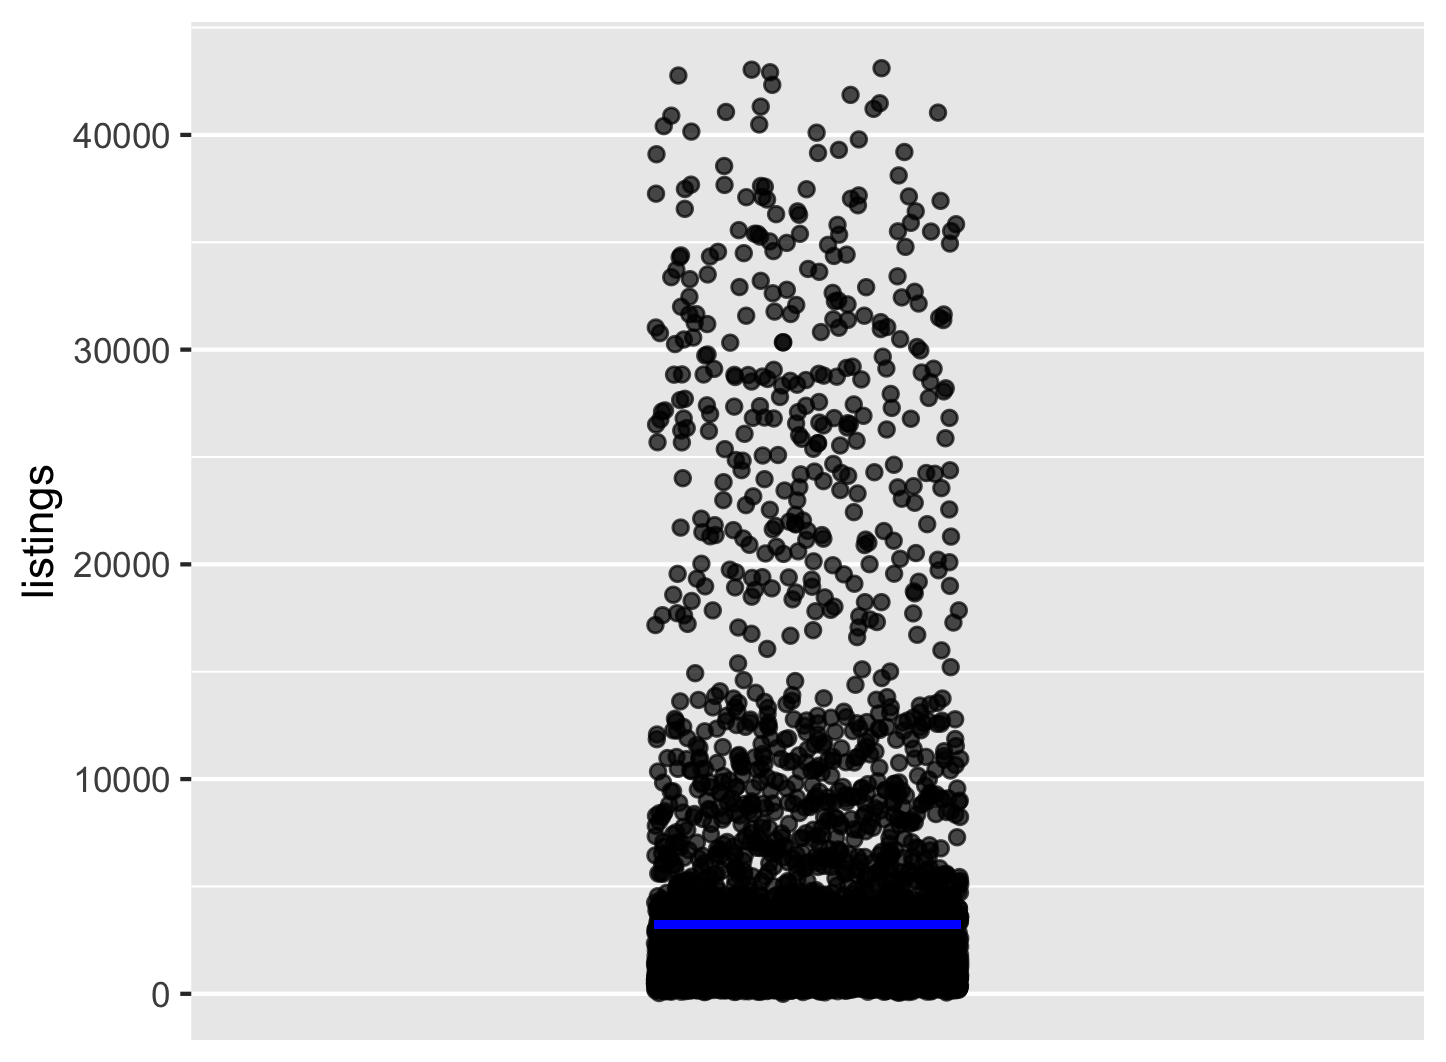
\includegraphics[width=0.7\linewidth,height=\textheight,keepaspectratio]{modules/04-more-on-models/../../images/fig-txhousing-listings-mean-model.png}

}

\caption{\label{fig-txhousing-listings-mean-model}Scatter plot of
\emph{listings} from the \emph{txhousing} data frame annotated with a
model: the model is the blue horizontal line at the average value of
listings (3217)}

\end{figure}%

Let us see one more example of visualizing a simple mean model.

The data frame \emph{Boston\_marathon} contains data about the results
of the Boston Marathon over the years.

Like we did with the \emph{txhousing} data frame, we should first
understand the data frame before processing it. Take a look at the
codebook for the \emph{Boston\_marathon} data frame and answer the
following questions. Try to recall how we got the codebook for
\emph{txhousing} and use the same approach here. The codebook is not too
informative, but just viewing it using View(Boston\_marathon) might tell
you what you need to know.

\begin{tcolorbox}[enhanced jigsaw, colback=white, leftrule=.75mm, toprule=.15mm, bottomtitle=1mm, breakable, coltitle=black, toptitle=1mm, title={Quick Check}, opacitybacktitle=0.6, colbacktitle=quarto-callout-note-color!10!white, arc=.35mm, left=2mm, colframe=quarto-callout-note-color-frame, titlerule=0mm, rightrule=.15mm, bottomrule=.15mm, opacityback=0]

How many variables does the data frame have?

\end{tcolorbox}

\begin{tcolorbox}[enhanced jigsaw, colback=white, leftrule=.75mm, toprule=.15mm, bottomtitle=1mm, breakable, coltitle=black, toptitle=1mm, title={Suggested answer}, opacitybacktitle=0.6, colbacktitle=quarto-callout-note-color!10!white, arc=.35mm, left=2mm, colframe=quarto-callout-note-color-frame, titlerule=0mm, rightrule=.15mm, bottomrule=.15mm, opacityback=0]

Six

\end{tcolorbox}

\begin{tcolorbox}[enhanced jigsaw, colback=white, leftrule=.75mm, toprule=.15mm, bottomtitle=1mm, breakable, coltitle=black, toptitle=1mm, title={Quick Check}, opacitybacktitle=0.6, colbacktitle=quarto-callout-note-color!10!white, arc=.35mm, left=2mm, colframe=quarto-callout-note-color-frame, titlerule=0mm, rightrule=.15mm, bottomrule=.15mm, opacityback=0]

What is the unit of observation? That is, what does a row tell us about?

\end{tcolorbox}

\begin{tcolorbox}[enhanced jigsaw, colback=white, leftrule=.75mm, toprule=.15mm, bottomtitle=1mm, breakable, coltitle=black, toptitle=1mm, title={Suggested answer}, opacitybacktitle=0.6, colbacktitle=quarto-callout-note-color!10!white, arc=.35mm, left=2mm, colframe=quarto-callout-note-color-frame, titlerule=0mm, rightrule=.15mm, bottomrule=.15mm, opacityback=0]

Each row tells us about the result of a year's race for a gender. The
unit of observation therefore is the result of a race in a year -- with
the races for males and females being considered as different races.

We have two rows for years starting from 1972 when women started
participating. Prior to that, from 1897 to 1971, we have only one row
per year.

\end{tcolorbox}

\begin{tcolorbox}[enhanced jigsaw, colback=white, leftrule=.75mm, toprule=.15mm, bottomtitle=1mm, breakable, coltitle=black, toptitle=1mm, title={Quick Check}, opacitybacktitle=0.6, colbacktitle=quarto-callout-note-color!10!white, arc=.35mm, left=2mm, colframe=quarto-callout-note-color-frame, titlerule=0mm, rightrule=.15mm, bottomrule=.15mm, opacityback=0]

Which column shows the finishing time?

\end{tcolorbox}

\begin{tcolorbox}[enhanced jigsaw, colback=white, leftrule=.75mm, toprule=.15mm, bottomtitle=1mm, breakable, coltitle=black, toptitle=1mm, title={Suggested answer}, opacitybacktitle=0.6, colbacktitle=quarto-callout-note-color!10!white, arc=.35mm, left=2mm, colframe=quarto-callout-note-color-frame, titlerule=0mm, rightrule=.15mm, bottomrule=.15mm, opacityback=0]

The variable \emph{time} shows the finishing time in seconds and the
colvariableumn \emph{minutes} shows it in minutes.

\end{tcolorbox}

\begin{tcolorbox}[enhanced jigsaw, colback=white, leftrule=.75mm, toprule=.15mm, bottomtitle=1mm, breakable, coltitle=black, toptitle=1mm, title={Quick Check}, opacitybacktitle=0.6, colbacktitle=quarto-callout-note-color!10!white, arc=.35mm, left=2mm, colframe=quarto-callout-note-color-frame, titlerule=0mm, rightrule=.15mm, bottomrule=.15mm, opacityback=0]

How can you verify the suggested answer from the previous question?

\end{tcolorbox}

\begin{tcolorbox}[enhanced jigsaw, colback=white, leftrule=.75mm, toprule=.15mm, bottomtitle=1mm, breakable, coltitle=black, toptitle=1mm, title={Suggested answer}, opacitybacktitle=0.6, colbacktitle=quarto-callout-note-color!10!white, arc=.35mm, left=2mm, colframe=quarto-callout-note-color-frame, titlerule=0mm, rightrule=.15mm, bottomrule=.15mm, opacityback=0]

Multiply \emph{minutes} by 60 and that should equal \emph{time}.
However, we cannot use the variable \emph{time} as it is not numerical.
(Take a close look.)

\end{tcolorbox}

Let us visualize a model for the variable \emph{minutes}. As before, we
generate the scatterplot and then annotate with a model. We changed the
data frame and the tilde expression.
Figure~\ref{fig-boston-marathon-minutes-model} shows the plot. The model
line is at \emph{minutes = 144}.

\begin{lstlisting}[language=R]
Boston_marathon |> 
  point_plot(minutes ~ 1, annot = "model",
             interval = "none")
\end{lstlisting}

\begin{figure}

\centering{

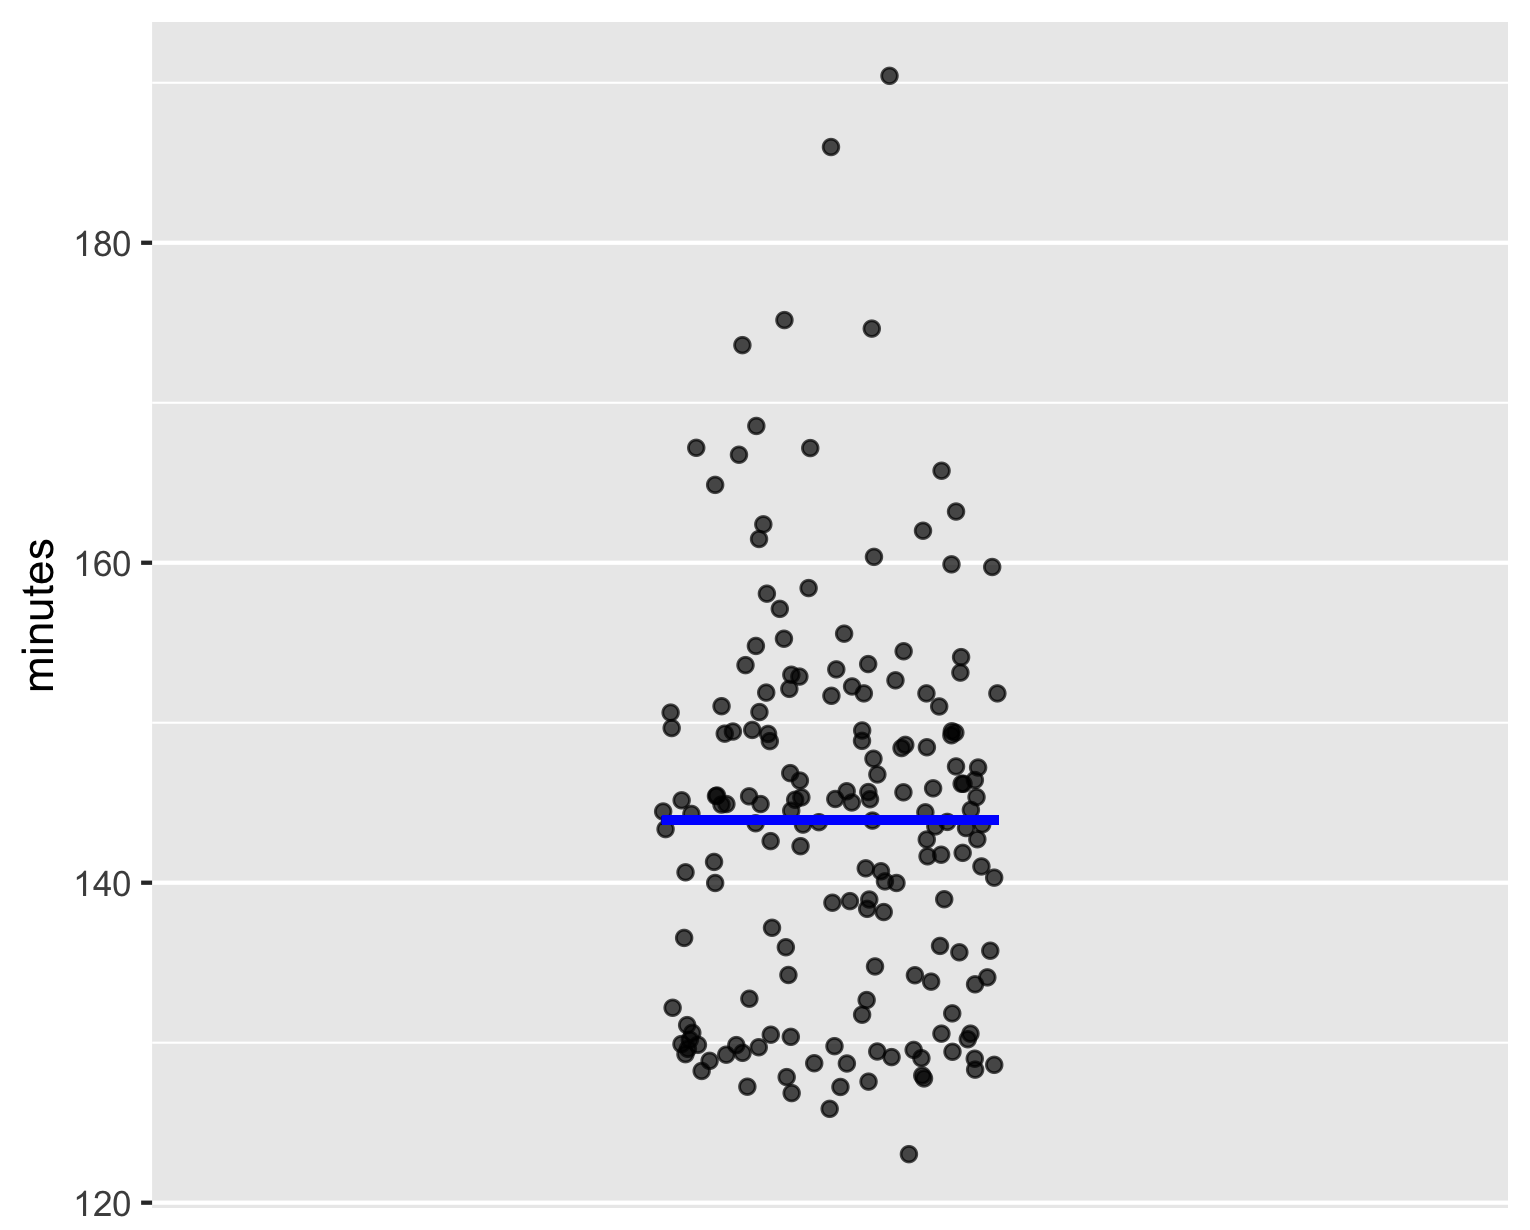
\includegraphics[width=0.7\linewidth,height=\textheight,keepaspectratio]{modules/04-more-on-models/../../images/fig-boston-marathon-minutes-model.png}

}

\caption{\label{fig-boston-marathon-minutes-model}Scatterplot of
\emph{minutes} from the \emph{Boston\_marathon} data frame annotated
with a model}

\end{figure}%

\section{Visualizing category mean models (single explanatory variable
that is
categorical)}\label{visualizing-category-mean-models-single-explanatory-variable-that-is-categorical}

We built a model for \emph{minutes} from the \emph{Boston\_marathon}
data frame assuming no explanatory variable. What if we used \emph{sex}
as the explanatory variable?
Figure~\ref{fig-boston-marathon-minutes-sex-model} shows the model. This
time we have a separate mean model for each sex.

\begin{lstlisting}[language=R]
Boston_marathon |> 
  point_plot(minutes ~ sex, annot = "model",
             interval = "none")
\end{lstlisting}

\begin{figure}

\centering{

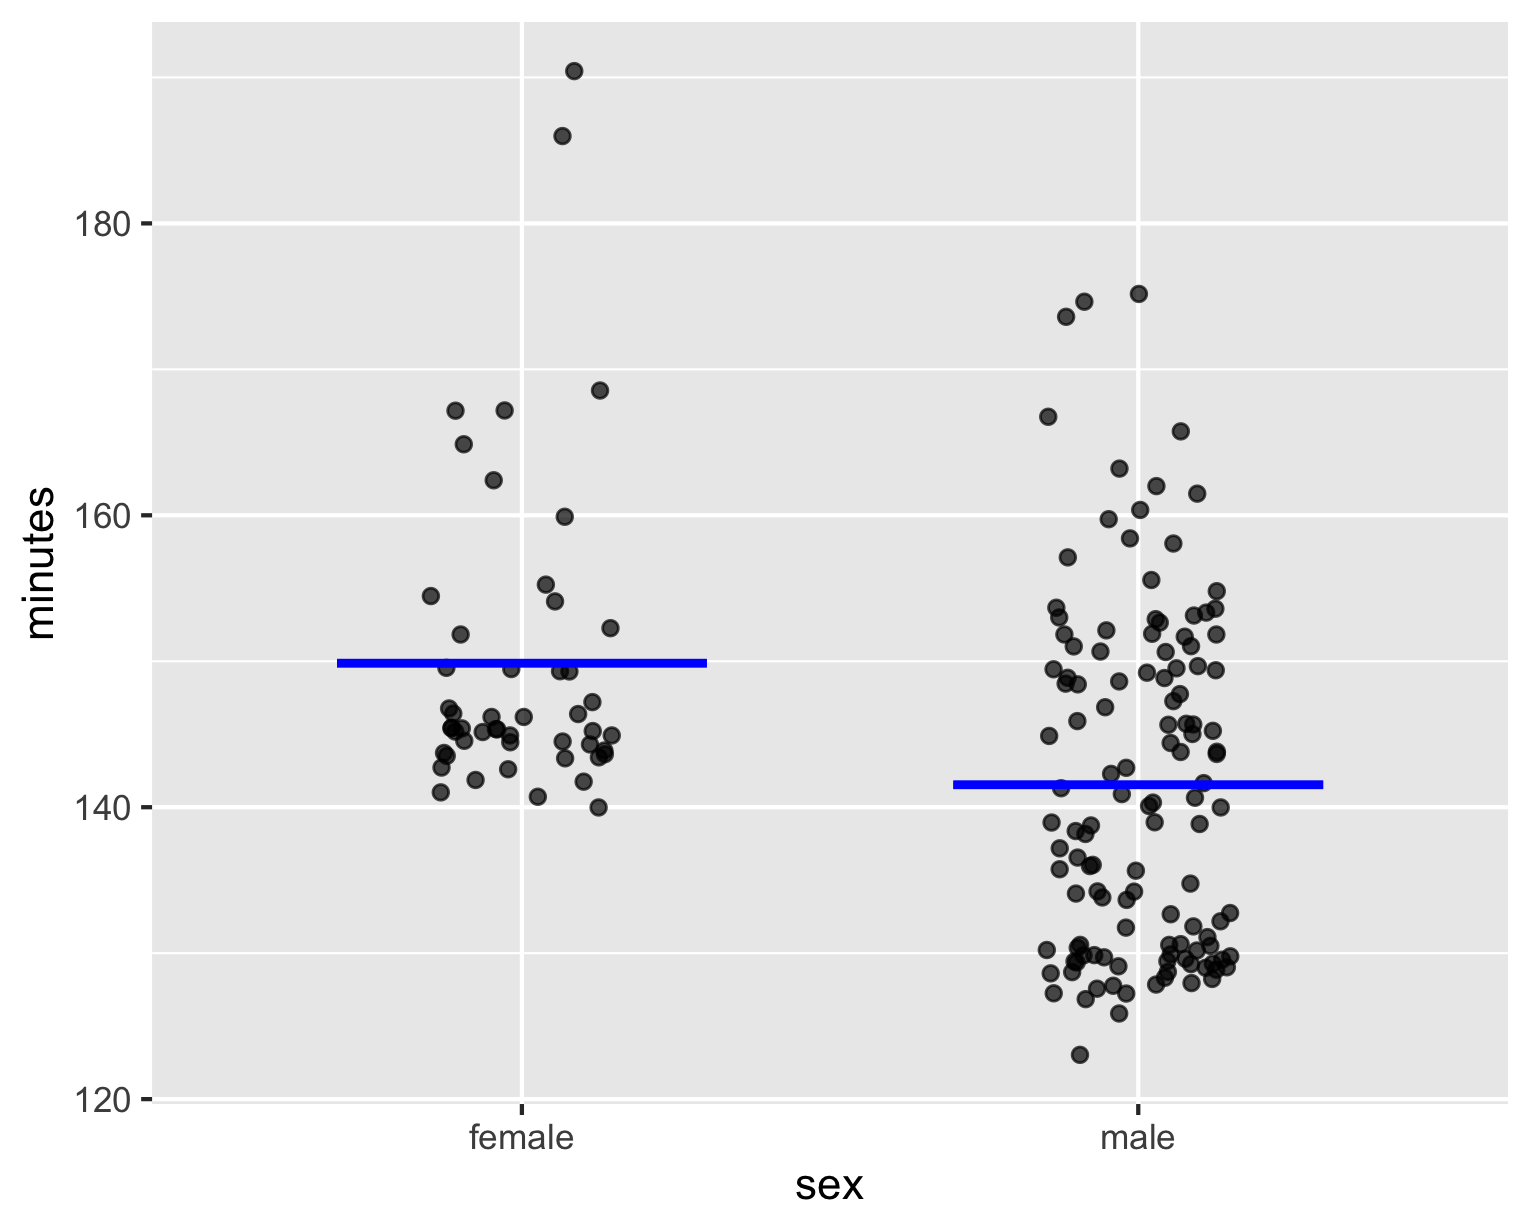
\includegraphics[width=0.7\linewidth,height=\textheight,keepaspectratio]{modules/04-more-on-models/../../images/fig-boston-marathon-minutes-sex-model.png}

}

\caption{\label{fig-boston-marathon-minutes-sex-model}Boston marathon
model for \emph{minutes} with \emph{sex} as the explanatory variabl}

\end{figure}%

For another example, we now use the \emph{mpg} data frame and plot a
model for the city. mileage (variable \emph{cty}) with the kind of drive
(variable \emph{drv}) as the explanatory variable.
Figure~\ref{fig-mpg-cty-drv-model} shows the plot. This time we see that
the model is the mean for each kind of drive.

\begin{lstlisting}[language=R]
mpg |> 
  point_plot(cty ~ drv, annot = "model", 
             interval = "none")
\end{lstlisting}

\begin{figure}

\centering{

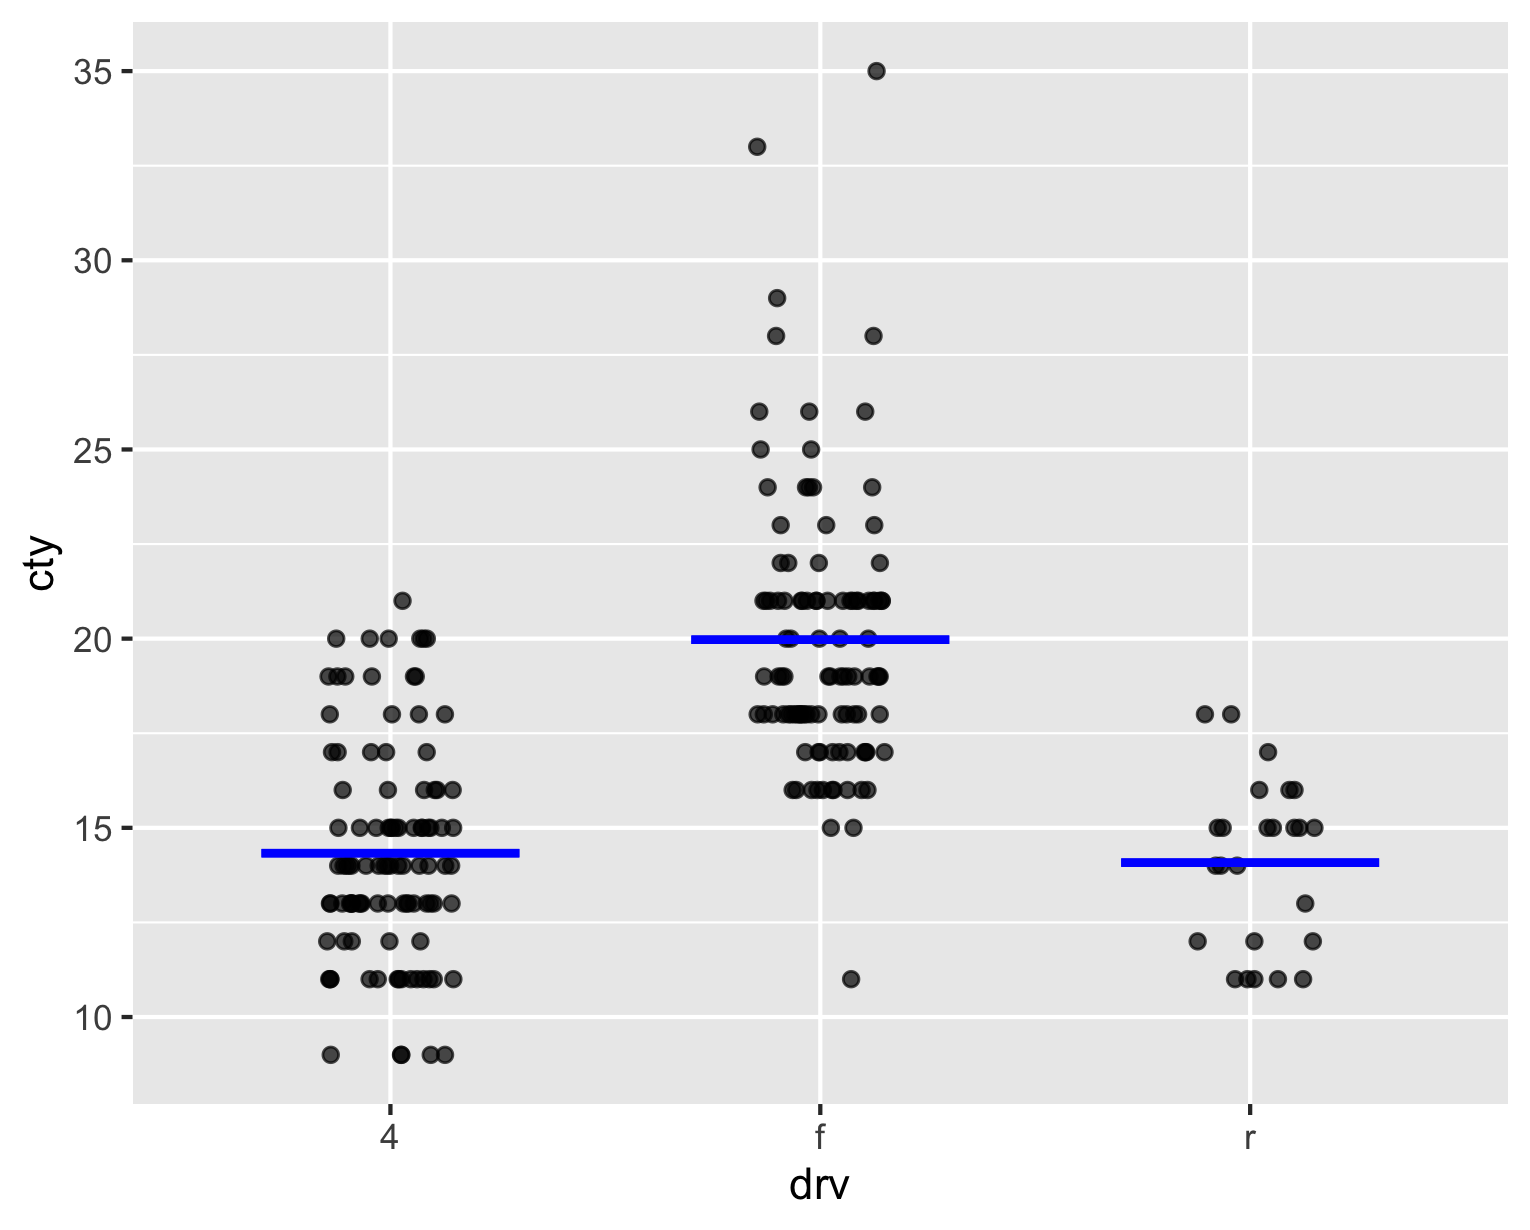
\includegraphics[width=0.7\linewidth,height=\textheight,keepaspectratio]{modules/04-more-on-models/../../images/fig-mpg-cty-drv-model.png}

}

\caption{\label{fig-mpg-cty-drv-model}Model of category means for
\emph{cty \textasciitilde{} drv} for the \emph{mpg} data frame}

\end{figure}%

\section{Visualizing least-squares line models (single explanatory
variable that is
numeric)}\label{visualizing-least-squares-line-models-single-explanatory-variable-that-is-numeric}

We use the \emph{Anthro\_F} data frame. Take a look at its codebook and
answer the following question.

\begin{tcolorbox}[enhanced jigsaw, colback=white, leftrule=.75mm, toprule=.15mm, bottomtitle=1mm, breakable, coltitle=black, toptitle=1mm, title={Quick Check}, opacitybacktitle=0.6, colbacktitle=quarto-callout-note-color!10!white, arc=.35mm, left=2mm, colframe=quarto-callout-note-color-frame, titlerule=0mm, rightrule=.15mm, bottomrule=.15mm, opacityback=0]

What is the unit of observation?

\end{tcolorbox}

\begin{tcolorbox}[enhanced jigsaw, colback=white, leftrule=.75mm, toprule=.15mm, bottomtitle=1mm, breakable, coltitle=black, toptitle=1mm, title={Suggested answer}, opacitybacktitle=0.6, colbacktitle=quarto-callout-note-color!10!white, arc=.35mm, left=2mm, colframe=quarto-callout-note-color-frame, titlerule=0mm, rightrule=.15mm, bottomrule=.15mm, opacityback=0]

Each row gives us information about a single college woman in the age
range 18-25. SO the unit of observation is a \emph{single college woman
in the age range 18-25}.

\end{tcolorbox}

We would like to visualize a model that predicts the body fat (variable
\emph{BFat}) with \emph{Wrist} as the explanatory variable.
Figure~\ref{fig-anthro-f-wrist-bfat-model} shows the scatterplot and the
least squares line.

\begin{lstlisting}[language=R]
 Anthro_F |> 
  point_plot(BFat ~ Wrist, annot = "model",
             interval = "none")
\end{lstlisting}

\begin{figure}

\centering{

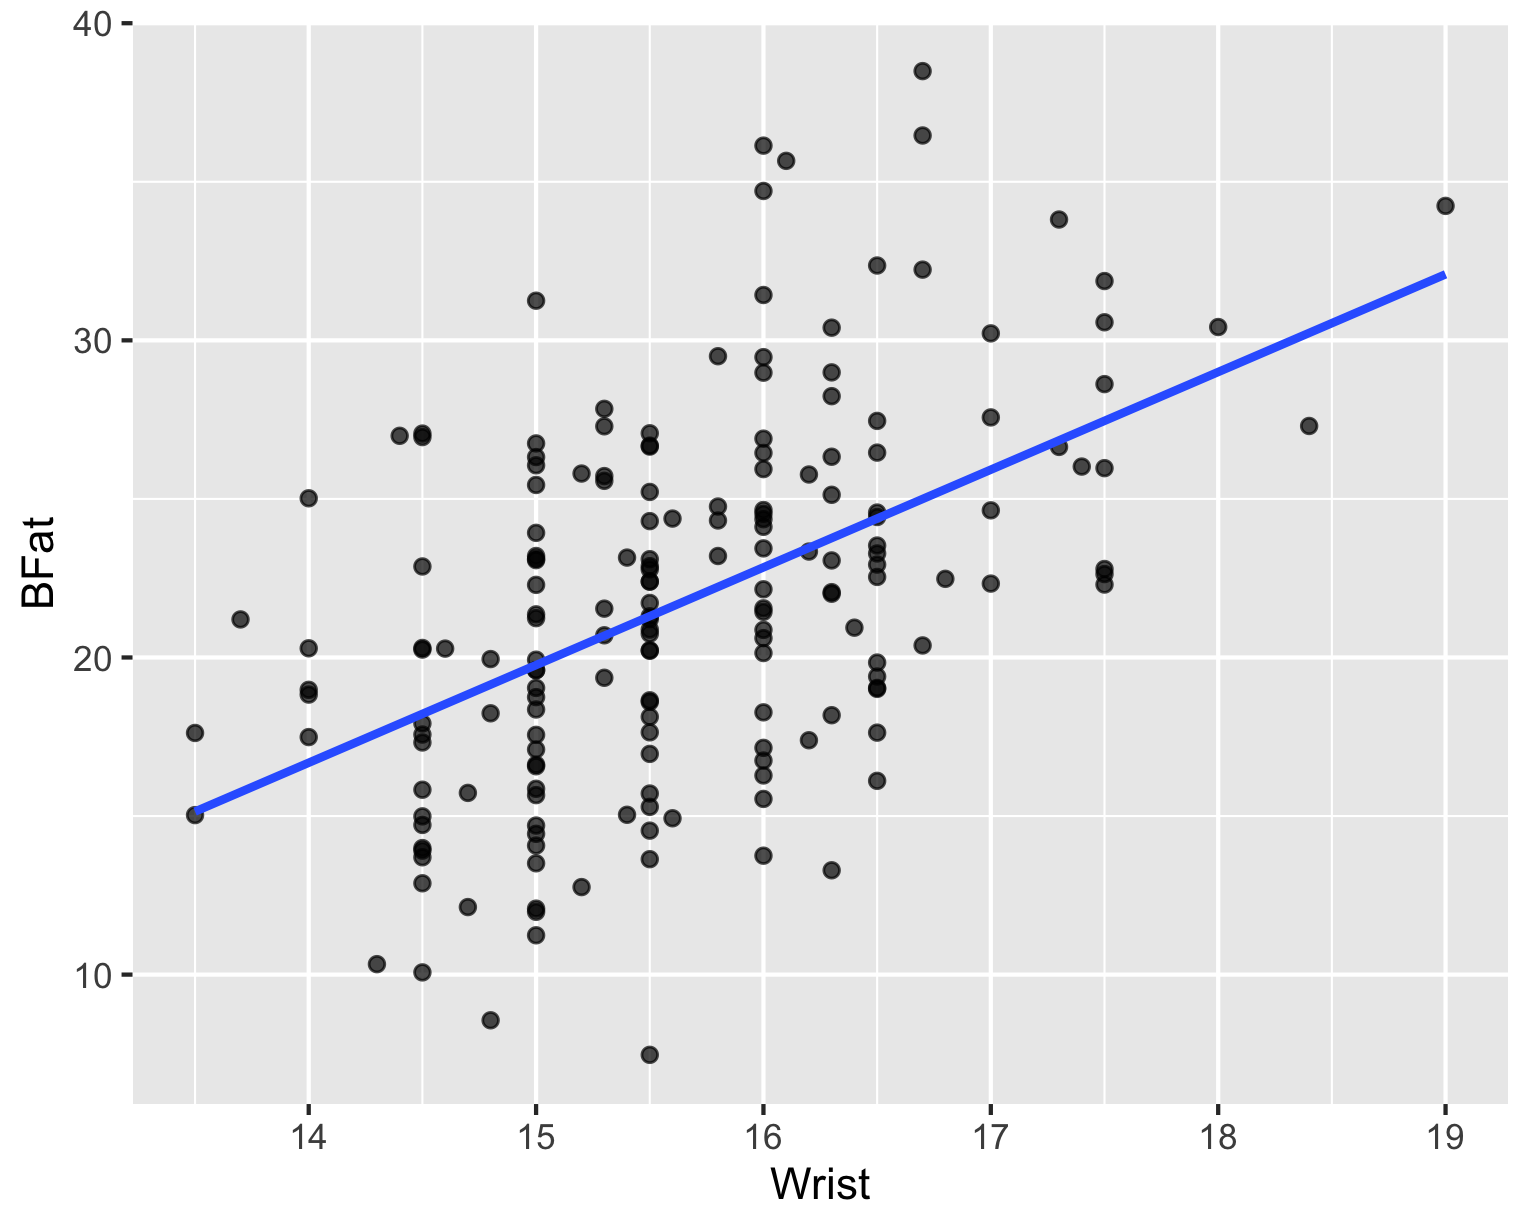
\includegraphics[width=0.7\linewidth,height=\textheight,keepaspectratio]{modules/04-more-on-models/../../images/fig-anthro-f-wrist-bfat-model.png}

}

\caption{\label{fig-anthro-f-wrist-bfat-model}Least squares line model
for the \emph{Anthro\_f} data frame: \emph{BFat} as the response
variable with \emph{Wrist} as the explanatory variable}

\end{figure}%

\chapter{Finding the Model Function}\label{sec-model-functions}

Our journey so far has introduced the idea of models and shown us the
intuition, and rationale behind models. We have also seen how to
visualize the models. However, although we have seen in bits and pieces
how we build models and reconstruct the model function from the R
output, we have not given it focussed attention.

This chapter closes the loop.

\section{Finding the model function for models with no explanatory
variables}\label{finding-the-model-function-for-models-with-no-explanatory-variables}

When we have a numerical outcome variable and no explanatory variable,
Chapter~\ref{sec-mean-model} showed us that the \emph{best} model would
be to predict the mean or average. We look at two ways of building such
models:

\begin{itemize}
\tightlist
\item
  building the model by explicitly computing the mean
\item
  using the model\_train function (our go to method from now on)
\end{itemize}

\subsection{Building mean models by explicitly computing the
mean}\label{building-mean-models-by-explicitly-computing-the-mean}

Do you remember how to compute the mean of a variable?

\begin{tcolorbox}[enhanced jigsaw, colback=white, leftrule=.75mm, toprule=.15mm, bottomtitle=1mm, breakable, coltitle=black, toptitle=1mm, title={Quick Check}, opacitybacktitle=0.6, colbacktitle=quarto-callout-note-color!10!white, arc=.35mm, left=2mm, colframe=quarto-callout-note-color-frame, titlerule=0mm, rightrule=.15mm, bottomrule=.15mm, opacityback=0]

Given a hypothetical data frame named \emph{dat} do you recall how to
compute the mean of one of its variables named \emph{col} using R?

\end{tcolorbox}

\begin{tcolorbox}[enhanced jigsaw, colback=white, leftrule=.75mm, toprule=.15mm, bottomtitle=1mm, breakable, coltitle=black, toptitle=1mm, title={Suggested answer}, opacitybacktitle=0.6, colbacktitle=quarto-callout-note-color!10!white, arc=.35mm, left=2mm, colframe=quarto-callout-note-color-frame, titlerule=0mm, rightrule=.15mm, bottomrule=.15mm, opacityback=0]

dat \textbar\textgreater{} summarize(avg\_col = mean(col))

\end{tcolorbox}

Using the \emph{txhousing} data frame, we can build a model for the
number of listings as follows:

\begin{lstlisting}[language=R]
txhousing |>
    summarize(avg_listings = mean(listings))
\end{lstlisting}

\begin{lstlisting}
# A tibble: 1 x 1
  avg_listings
         <dbl>
1           NA
\end{lstlisting}

Why is the result not a number? Why did we get \emph{NA}?

You might recall from Section~\ref{sec-missing-values} that \emph{NA}
means missing value. Why is the mean of \emph{listings} a missing value?
The \emph{txhousing} data frame has some missing values in the column
\emph{listings}. As a result, our code is unable to compute the average.
Suppose I asked you what is 2 + 3, you can say ``5.'' since you have
both the numbers that you want to add up.

However, if I asked you what is \emph{NA} + 5? You cannot say what it is
because you do not know the values of the two numbers you are trying to
sum. In general, whenever \emph{NA} is involved in an operation, the
result is always \emph{NA}.

This is very inconvenient. Wht does the system simply not ignore the
\emph{NA}s and compute the average of the remaining numbers? By default
it does not do that, but we can make the system do that in the following
way.

\begin{lstlisting}[language=R]
txhousing |>
    summarize(avg_listings = mean(listings, na.rm = TRUE))
\end{lstlisting}

\begin{lstlisting}
# A tibble: 1 x 1
  avg_listings
         <dbl>
1        3217.
\end{lstlisting}

When you add ``na.rm = TRUE'', R leaves out the missing values and
computes the average of the rest. Remember, R is case sensitive and so
you have to type ``na.rm'' in lowercase and ``TRUE'' in uppercase.
Otherwise you will get an error.

So we saw that the mean of \emph{listings} is 3217 and that is our model
value.

We can write the model function as
Equation~\ref{eq-txhousing-listings-mean-model}

\begin{equation}\phantomsection\label{eq-txhousing-listings-mean-model}{
\widehat{\text{listings}} = 3217
}\end{equation}

We have built the mean model by explicitly writing code to compute the
average.

\begin{tcolorbox}[enhanced jigsaw, colback=white, leftrule=.75mm, toprule=.15mm, bottomtitle=1mm, breakable, coltitle=black, toptitle=1mm, title={Quick Check}, opacitybacktitle=0.6, colbacktitle=quarto-callout-note-color!10!white, arc=.35mm, left=2mm, colframe=quarto-callout-note-color-frame, titlerule=0mm, rightrule=.15mm, bottomrule=.15mm, opacityback=0]

In Chapter~\ref{sec-mean-model}, we saw a situation where the interns
had to find a single fixed number to represent the number of customers
who will show up at a kiosk on any day. What could be a business
analogue of that in the \emph{listings} example from the
\emph{txhousing} data frame?

\end{tcolorbox}

\begin{tcolorbox}[enhanced jigsaw, colback=white, leftrule=.75mm, toprule=.15mm, bottomtitle=1mm, breakable, coltitle=black, toptitle=1mm, title={Suggested answer}, opacitybacktitle=0.6, colbacktitle=quarto-callout-note-color!10!white, arc=.35mm, left=2mm, colframe=quarto-callout-note-color-frame, titlerule=0mm, rightrule=.15mm, bottomrule=.15mm, opacityback=0]

The analogue would be: We need to build a model for the number of
listings in a typical month, and we were allowed to give just a single
fixed number for it. Also, like before, bigger errors are penalized more
strongly through squaring prediction errors.

\end{tcolorbox}

\subsection{\texorpdfstring{Building the mean model using
\emph{model\_train}}{Building the mean model using model\_train}}\label{building-the-mean-model-using-model_train}

The \emph{model\_train} function greatly simplifies the process of
building models irrespective of the form of the model. We do not need to
worry about what types of explanatory variables and how many of them are
involved.

Let us see how to use it to build the model for \emph{listings} with no
explanatory variables.

\begin{lstlisting}[language=R]
txhousing |>
    model_train(listings ~ 1)
\end{lstlisting}

\begin{lstlisting}
A trained model relating the response variable "listings"
to explanatory variable "".

To see relevant details, use model_eval(), conf_interval(),
R2(), regression_summary(), anova_summary(), or model_plot(),
or the native R model-reporting functions.
\end{lstlisting}

We have built the model, but the output does not give us any details
about the model to enable us to reconstruct the model function.

We can fix that easily by calling another function -- \emph{coef} -- to
get the model \emph{coefficients}.

\begin{lstlisting}[language=R]
txhousing |>
    model_train(listings ~ 1) |>
    coef()
\end{lstlisting}

\begin{lstlisting}
(Intercept) 
       3217 
\end{lstlisting}

The output says that the \emph{intercept} is 3217 (rounded). The model
output does not show any other coefficients because we do not have any
explanatory variables. From this, we can reconstruct the model function
as Equation~\ref{eq-txhousing-listings-mean-model-copy} (same as
Figure~\ref{fig-txhousing-listings-mean-model}). We explain below
exactly how we went from the coefficients in the output to
Equation~\ref{eq-txhousing-listings-mean-model-copy}.

\begin{equation}\phantomsection\label{eq-txhousing-listings-mean-model-copy}{
\widehat{\text{listings}} = 3217
}\end{equation}

You might recall from Chapter~\ref{sec-best-fit-line} that in general
when we have a single explanatory variable, we are trying to find the
best values for \emph{a} and \emph{b} in an equation of the from that
Equation~\ref{eq-generic} provides to compute an estimated value for the
outcome variable (hence the \emph{hat})

\begin{equation}\phantomsection\label{eq-generic}{
\widehat{\text{outcome}} = a + b\times\text{explanatory\_var}
}\end{equation}

The \emph{intercept} in the model coefficients output by the \emph{coef}
function corresponds to \emph{a}. If there is another coefficient in the
output that corresponds to \emph{b}. In the current example we have only
the \emph{intercept} and no other coefficient and so we use only
\emph{a} in reconstructing the model function as
Equation~\ref{eq-txhousing-listings-mean-model-copy}.

Let us consider another example using the \emph{mpg} data frame. We will
now build a model for \emph{cty} with no explanatory variables.

\begin{lstlisting}[language=R]
mpg |> 
  model_train(cty ~ 1) |> 
  coef()
\end{lstlisting}

\begin{lstlisting}
(Intercept) 
       16.9 
\end{lstlisting}

We see that the \emph{intercept} is 16.86 (rounded). This is, of course,
the mean of \emph{cty}. Equation~\ref{eq-mpg-cty-mean-model} shows the
model function.

\begin{equation}\phantomsection\label{eq-mpg-cty-mean-model}{
\widehat{\text{cty}} = 16.9
}\end{equation}

\begin{tcolorbox}[enhanced jigsaw, colback=white, leftrule=.75mm, toprule=.15mm, bottomtitle=1mm, breakable, coltitle=black, toptitle=1mm, title={Quick Check}, opacitybacktitle=0.6, colbacktitle=quarto-callout-note-color!10!white, arc=.35mm, left=2mm, colframe=quarto-callout-note-color-frame, titlerule=0mm, rightrule=.15mm, bottomrule=.15mm, opacityback=0]

Can you think of a business scenario where this sort of model might be
used?

\end{tcolorbox}

\begin{tcolorbox}[enhanced jigsaw, colback=white, leftrule=.75mm, toprule=.15mm, bottomtitle=1mm, breakable, coltitle=black, toptitle=1mm, title={Suggested answer}, opacitybacktitle=0.6, colbacktitle=quarto-callout-note-color!10!white, arc=.35mm, left=2mm, colframe=quarto-callout-note-color-frame, titlerule=0mm, rightrule=.15mm, bottomrule=.15mm, opacityback=0]

If a company had a fleet of cars and needed to estimate something based
on the city mileage of the fleet as a whole and we had to settle on just
a single representative number for the whole fleet, then the average
would be the best -- assuming again that bigger errors are more heavily
penalized.

\end{tcolorbox}

Let us close out with another example from the \emph{Anthro\_F} data
frame to estimate body fat (variable *BFat) with no explanatory
variables.

\begin{lstlisting}[language=R]
Anthro_F |> 
  model_train(BFat ~ 1) |> 
  coef()
\end{lstlisting}

\begin{lstlisting}
(Intercept) 
       21.8 
\end{lstlisting}

This shows an \emph{intercept} of 21.8 (rounded).
Equation~\ref{eq-anthro-f-bfat-model} shows the model function.

\begin{equation}\phantomsection\label{eq-anthro-f-bfat-model}{
\widehat{\text{BFat}} = 21.8
}\end{equation}

\begin{tcolorbox}[enhanced jigsaw, colback=white, leftrule=.75mm, toprule=.15mm, bottomtitle=1mm, breakable, coltitle=black, toptitle=1mm, title={Quick Check}, opacitybacktitle=0.6, colbacktitle=quarto-callout-note-color!10!white, arc=.35mm, left=2mm, colframe=quarto-callout-note-color-frame, titlerule=0mm, rightrule=.15mm, bottomrule=.15mm, opacityback=0]

As before, what might be a usage scenario for this model?

\end{tcolorbox}

\begin{tcolorbox}[enhanced jigsaw, colback=white, leftrule=.75mm, toprule=.15mm, bottomtitle=1mm, breakable, coltitle=black, toptitle=1mm, title={Suggested answer}, opacitybacktitle=0.6, colbacktitle=quarto-callout-note-color!10!white, arc=.35mm, left=2mm, colframe=quarto-callout-note-color-frame, titlerule=0mm, rightrule=.15mm, bottomrule=.15mm, opacityback=0]

If, for some reason we needed a representative number -- a single number
-- for the body fat of a group of college age females in the age range
18-25 (as the data set on which we based the model), then this model
would work.

\end{tcolorbox}

\begin{tcolorbox}[enhanced jigsaw, colback=white, leftrule=.75mm, toprule=.15mm, bottomtitle=1mm, breakable, coltitle=black, toptitle=1mm, title=\textcolor{quarto-callout-tip-color}{\faLightbulb}\hspace{0.5em}{Steps to build the model function for models with no explanatory
variable}, opacitybacktitle=0.6, colbacktitle=quarto-callout-tip-color!10!white, arc=.35mm, left=2mm, colframe=quarto-callout-tip-color-frame, titlerule=0mm, rightrule=.15mm, bottomrule=.15mm, opacityback=0]

\begin{enumerate}
\def\labelenumi{\arabic{enumi}.}
\tightlist
\item
  Determine the tilde expression for your model (like listings
  \textasciitilde{} 1, or some such)
\item
  Pipe the data frame to the \emph{model\_train} function and pass the
  tilde expression as well
\item
  Pipe the output of the \emph{model\_train} function to the
  \emph{coef()} function
\item
  Look at the results and map the \emph{intercept} to \emph{a}
\item
  Construct the model function by substituting the name of the outcome
  variable and the value of \emph{a} in the equation with the intercept:
  \[
  \widehat{\text{outcome\_var}} = \text{a}
  \]
\end{enumerate}

\end{tcolorbox}

\section{Finding the model function for models with one explanatory
variable
alone}\label{finding-the-model-function-for-models-with-one-explanatory-variable-alone}

Mirroring the process from the previous section, we have two ways of
building these models:

\begin{itemize}
\tightlist
\item
  building the model by explicitly computing the category means
\item
  using the model\_train function (our go to method from now on)
\end{itemize}

\subsection{Building category mean models by explicitly computing
category
means}\label{building-category-mean-models-by-explicitly-computing-category-means}

Let us use the \emph{Boston\_marathon} data frame to build a model for
\emph{minutes} with \emph{sex} as the explanatory variable.

\begin{lstlisting}[language=R]
Boston_marathon |> 
  summarize(avg_minutes = mean(minutes), .by = sex)
\end{lstlisting}

\begin{lstlisting}
# A tibble: 2 x 2
  sex    avg_minutes
  <chr>        <dbl>
1 male          142.
2 female        150.
\end{lstlisting}

In the above code, if we had not used ``.by = sex'', we would have got
the overall mean. But using ``.by = sex'' computes a separate mean for
each value of \emph{sex}.

We now have the mean of \emph{minutes} for each sex and can build the
model function as:

\begin{equation}\phantomsection\label{eq-boston-marathon-minutes-sex-model}{
\widehat{\text{minutes}} =
\begin{cases}
142 & \text{if } \text{sex} = \text{"male"} \\
150 & \text{if } \text{sex} = \text{"female"}
\end{cases}
}\end{equation}

As before, this is needlessly cumbersome. We can do this using the
\emph{model\_train} function like before.

\begin{lstlisting}[language=R]
Boston_marathon |> 
  model_train(minutes ~ sex) |> 
  coef()
\end{lstlisting}

\begin{lstlisting}
(Intercept)     sexmale 
     149.87       -8.33 
\end{lstlisting}

The output looks a bit different now. We have the \emph{intercept} as
before. But we have a single coefficient named \emph{sexmale}.

When we have categorical explanatory variables, the \emph{model\_train}
function reports coefficients a bit differently than what we did
earlier.

Our explanatory variable has two possible values, \emph{female} and
\emph{male}. The intercept represents the model value for one of these
-- typically, the alphabetically lowest one -- in this case
\emph{female} as \emph{f} comes alphabetically before \emph{m}.

So the coefficient 149.86, which we wil round to 10 is the model value
for \emph{female} as our earlier computations also showed. This is the
base value. The coefficient for \emph{sexmale} shows the coefficient
value for \emph{male} relative to that for the base. This means that the
coefficient for \emph{male} is \emph{less} (because it is negative) than
that for female by 8.33. The coefficient for \emph{male} is
approximately 142.

So we can construct the model function as:

\begin{equation}\phantomsection\label{eq-boston-marathon-minutes-sex-model-1}{
\widehat{\text{minutes}} =
\begin{cases}
142 & \text{if } \text{sex} = \text{"female"} \\
142 & - 8\,\, \text{if } \text{sex} = \text{"male"}
\end{cases}
}\end{equation}

Equation~\ref{eq-boston-marathon-minutes-sex-model-1} is effectively the
same as Equation~\ref{eq-boston-marathon-minutes-sex-model}, but written
slightly differently.

You should read it as, if \emph{sex} is ``female'' then the model value
is 150. If \emph{sex} is ``male'' then the model value is 8 minutes
lower (negative sign).

Does this make sense? It does, because we know that males run slightly
faster than females and so their finishing time will be lower.

\begin{tcolorbox}[enhanced jigsaw, colback=white, leftrule=.75mm, toprule=.15mm, bottomtitle=1mm, breakable, coltitle=black, toptitle=1mm, title={Quick Check}, opacitybacktitle=0.6, colbacktitle=quarto-callout-note-color!10!white, arc=.35mm, left=2mm, colframe=quarto-callout-note-color-frame, titlerule=0mm, rightrule=.15mm, bottomrule=.15mm, opacityback=0]

What would be the use case scenario for this model?

\end{tcolorbox}

\begin{tcolorbox}[enhanced jigsaw, colback=white, leftrule=.75mm, toprule=.15mm, bottomtitle=1mm, breakable, coltitle=black, toptitle=1mm, title={Suggested answer}, opacitybacktitle=0.6, colbacktitle=quarto-callout-note-color!10!white, arc=.35mm, left=2mm, colframe=quarto-callout-note-color-frame, titlerule=0mm, rightrule=.15mm, bottomrule=.15mm, opacityback=0]

If the race organizers are planning to do something based on the typical
race completion time and can do something different for male and female
participants, then the average finishing times for each gender would be
a good model.

\end{tcolorbox}

Let us consider one more example using the \emph{acct\_type\_balance}
data frame with \emph{balance} as the outcome variable and
\emph{bank\_account\_type} as the explanatory variable.

\begin{lstlisting}[language=R]
acct_type_balance |> 
  model_train(balance ~ bank_account_type) |> 
  coef()
\end{lstlisting}

\begin{lstlisting}
             (Intercept) bank_account_typeSavings 
                    4901                     1016 
\end{lstlisting}

The output shows the intercept as 4901. Our explanatory variable
\emph{bank\_account\_type} has two possible values \emph{Savings} and
\emph{Checking}. From the previous example, we know that the
\emph{coef()} function will treat one of these as the base.

\begin{tcolorbox}[enhanced jigsaw, colback=white, leftrule=.75mm, toprule=.15mm, bottomtitle=1mm, breakable, coltitle=black, toptitle=1mm, title={Quick Check}, opacitybacktitle=0.6, colbacktitle=quarto-callout-note-color!10!white, arc=.35mm, left=2mm, colframe=quarto-callout-note-color-frame, titlerule=0mm, rightrule=.15mm, bottomrule=.15mm, opacityback=0]

Which account type will it treat as the base? \emph{Checking} or
\emph{Savings}?

\end{tcolorbox}

\begin{tcolorbox}[enhanced jigsaw, colback=white, leftrule=.75mm, toprule=.15mm, bottomtitle=1mm, breakable, coltitle=black, toptitle=1mm, title={Suggested answer}, opacitybacktitle=0.6, colbacktitle=quarto-callout-note-color!10!white, arc=.35mm, left=2mm, colframe=quarto-callout-note-color-frame, titlerule=0mm, rightrule=.15mm, bottomrule=.15mm, opacityback=0]

*Checking** because ``C'' is alphabetically before ``S''.

\end{tcolorbox}

\emph{Checking} is the base and its average is reported as the
\emph{intercept} and the model value for \emph{Savings} is reported
relative to the model value for \emph{Checking}.

The model function therefore becomes:

\begin{equation}\phantomsection\label{eq-bank-acct-type-bal-model}{
\widehat{\text{balance}} =
\begin{cases}
4901 & \text{if } \text{bank\_account\_type} = \text{"Checking"} \\
4901 & + 1016\,\, \text{if } \text{bank\_account\_type} = \text{"Savings"}
\end{cases}
}\end{equation}

The model says that savings accounts generally have a higher account
balance than checking accounts. Makes sense.

\begin{tcolorbox}[enhanced jigsaw, colback=white, leftrule=.75mm, toprule=.15mm, bottomtitle=1mm, breakable, coltitle=black, toptitle=1mm, title=\textcolor{quarto-callout-tip-color}{\faLightbulb}\hspace{0.5em}{Steps to build the model function for models with one categorical
explanatory variable}, opacitybacktitle=0.6, colbacktitle=quarto-callout-tip-color!10!white, arc=.35mm, left=2mm, colframe=quarto-callout-tip-color-frame, titlerule=0mm, rightrule=.15mm, bottomrule=.15mm, opacityback=0]

\begin{enumerate}
\def\labelenumi{\arabic{enumi}.}
\tightlist
\item
  Determine the tilde expression for your model (like balance
  \textasciitilde{} bank\_account\_type, or some such)
\item
  Pipe the data frame to the \emph{model\_train} function and pass the
  tilde expression as well
\item
  Pipe the output of the \emph{model\_train} function to the
  \emph{coef()} function
\item
  Find which category has been used as the base and note the intercept
\item
  Note the coefficients for each of the other categories
\item
  Construct the model function by substituting the name of the outcome
  variable, and the value of the intercept in the following equation.
\item
  Then add conditions for each additional category suitably substituting
  the appropriate category names. \[
  \widehat{\text{outcome}} =
  \begin{cases}
  intercept & \text{if } \text{explanatory variable} = \text{base category} \\
  intercept & + \,\text{coef1} \,\, \text{if } \text{explanatory variable} = \text{"category 1"} \\
  intercept & +\, \text{coef2} \,\, \text{if } \text{explanatory variable} = \text{"category 2"} \\
  intercept & +\, \text{coef3} \,\, \text{if } \text{explanatory variable} = \text{"category 3"}
  \end{cases}
  \]
\end{enumerate}

\end{tcolorbox}

\section{Finding the model function for models with a single numerical
explanatory
variable}\label{finding-the-model-function-for-models-with-a-single-numerical-explanatory-variable}

Unlike the two mean models, we have no direct computation approach. We
will just use the \emph{model\_train} function.

We will build a model using the \emph{mpg} data frame with the highway
mileage (variable \emph{hwy}) as the outcome variable and the engine
displacement (\emph{displ}) as the explanatory variable.

\begin{lstlisting}[language=R]
mpg |> 
  model_train(hwy ~ displ) |> 
  coef()
\end{lstlisting}

\begin{lstlisting}
(Intercept)       displ 
      35.70       -3.53 
\end{lstlisting}

As before, we substitute the ``intercept* for \emph{a} and in the case
of a numerical explanatory variable, we substitute the other coefficient
for \emph{b}.

Equation~\ref{eq-mpg-hwy-displ-model} shows the model function.

\begin{equation}\phantomsection\label{eq-mpg-hwy-displ-model}{
\widehat{\text{hwy}} = 36 - 3.5\times \text{displ}
}\end{equation}

Let us see another example. We use the \emph{Hill\_racing} data frame to
build a model with \emph{time} (finishing time measured in seconds) as
the outcome variable, and)\emph{distance} (measured in km) as the
explanatory variable.

\begin{lstlisting}[language=R]
Hill_racing |> 
  model_train(time ~ distance) |> 
  coef()
\end{lstlisting}

\begin{lstlisting}
(Intercept)    distance 
       -211         381 
\end{lstlisting}

We see that the \emph{intercept} is -211. The coefficient for
\emph{distance} is 381.

Let us build the model function before talking about the crazy-seeming
negative \emph{intercept}.

\begin{equation}\phantomsection\label{eq-hill-racing-time-distance-model}{
\widehat{\text{time}} = -211 + 381\times \text{distance}
}\end{equation}

Does it make sense that the coefficient for \emph{distance} is positive?
Per Equation~\ref{eq-hill-racing-time-distance-model}, as
\emph{distance} increases, the estimated \emph{time} will increase. This
makes sense.

What about the \emph{intercept} of -211?

From Equation~\ref{eq-hill-racing-time-distance-model}, we see that if
there is a hypothetical race with distance of 0 km, then the model says
that people will finish the race 211 seconds before the race starts!

Obviously that makes no sense if time works as it does in the normal
world. What is going on?

Models are approximate and we can only expect reasonable results within
the range of data on which they were built. We need to be wary of
interpreting models outside of their scope. In our dataset, the shortest
race is 1.1 km and the average is 10.7 km.

For the 1.1 km race, the model predicts a time of 208 seconds or around
3.5 minutes, which seems reasonable -- given that these are ``hill''
races.

\begin{tcolorbox}[enhanced jigsaw, colback=white, leftrule=.75mm, toprule=.15mm, bottomtitle=1mm, breakable, coltitle=black, toptitle=1mm, title={Quick Check}, opacitybacktitle=0.6, colbacktitle=quarto-callout-note-color!10!white, arc=.35mm, left=2mm, colframe=quarto-callout-note-color-frame, titlerule=0mm, rightrule=.15mm, bottomrule=.15mm, opacityback=0]

What would be a scenario where this model can help?

\end{tcolorbox}

\begin{tcolorbox}[enhanced jigsaw, colback=white, leftrule=.75mm, toprule=.15mm, bottomtitle=1mm, breakable, coltitle=black, toptitle=1mm, title={Suggested answer}, opacitybacktitle=0.6, colbacktitle=quarto-callout-note-color!10!white, arc=.35mm, left=2mm, colframe=quarto-callout-note-color-frame, titlerule=0mm, rightrule=.15mm, bottomrule=.15mm, opacityback=0]

The organizers are getting ready to conduct the races again. Now, they
want to give an estimated completion time (one single number) for each
race. They can use this model to find this time based on the distance of
each race.

\end{tcolorbox}

\begin{tcolorbox}[enhanced jigsaw, colback=white, leftrule=.75mm, toprule=.15mm, bottomtitle=1mm, breakable, coltitle=black, toptitle=1mm, title=\textcolor{quarto-callout-tip-color}{\faLightbulb}\hspace{0.5em}{Steps to build the model function for models with one numerical
explanatory variable}, opacitybacktitle=0.6, colbacktitle=quarto-callout-tip-color!10!white, arc=.35mm, left=2mm, colframe=quarto-callout-tip-color-frame, titlerule=0mm, rightrule=.15mm, bottomrule=.15mm, opacityback=0]

\begin{enumerate}
\def\labelenumi{\arabic{enumi}.}
\tightlist
\item
  Determine the tilde expression for your model (like hwy
  \textasciitilde{} displ, or some such)
\item
  Pipe the data frame to the \emph{model\_train} function and pass the
  tilde expression as well
\item
  Pipe the output of the \emph{model\_train} function to the
  \emph{coef()} function
\item
  Note the \emph{intercept} and the \emph{coefficient} for the
  explanatory variable (expl\_coeff)
\item
  Construct the model function by substituting the name of the outcome
  variable, and the value of the intercept in the following equation.
\item
  Then add conditions for each additional category suitably substituting
  the appropriate category names. \[
  \widehat{\text{outcome}} = \text{intercept} + \text{expl\_var\_coeff}\times\text{explanatory variable}
  \]
\end{enumerate}

\end{tcolorbox}

\chapter{Amanda's New Challenge}\label{sec-num-cat-explanatories}

In prior chapters we have looked at three different situations in the
specific context of Amanda's kiosks.
Table~\ref{tbl-first-three-model-types-kiosk-context} shows the
scenarios and the models we found for each.

\begin{longtable}[]{@{}
  >{\raggedright\arraybackslash}p{(\linewidth - 4\tabcolsep) * \real{0.4667}}
  >{\raggedright\arraybackslash}p{(\linewidth - 4\tabcolsep) * \real{0.2267}}
  >{\raggedright\arraybackslash}p{(\linewidth - 4\tabcolsep) * \real{0.3067}}@{}}
\caption{Model types we have looked at so far for the kiosk
scenarios}\label{tbl-first-three-model-types-kiosk-context}\tabularnewline
\toprule\noalign{}
\begin{minipage}[b]{\linewidth}\raggedright
Response variable
\end{minipage} & \begin{minipage}[b]{\linewidth}\raggedright
Explanatory var
\end{minipage} & \begin{minipage}[b]{\linewidth}\raggedright
Best model
\end{minipage} \\
\midrule\noalign{}
\endfirsthead
\toprule\noalign{}
\begin{minipage}[b]{\linewidth}\raggedright
Response variable
\end{minipage} & \begin{minipage}[b]{\linewidth}\raggedright
Explanatory var
\end{minipage} & \begin{minipage}[b]{\linewidth}\raggedright
Best model
\end{minipage} \\
\midrule\noalign{}
\endhead
\bottomrule\noalign{}
\endlastfoot
Num customers, one for both kiosks & None & Mean customers \\
Num customers, one per kiosk & Kiosk location & Mean for each kiosk \\
Number of customers & Temperature & Least squares line \\
\end{longtable}

Table~\ref{tbl-first-three-model-types-generic} summarizes the
situations in more generic terms than the specific kiosk context and the
best model for each. (Recall that in this book we consider only
numerical response variables.)

\begin{longtable}[]{@{}
  >{\raggedright\arraybackslash}p{(\linewidth - 4\tabcolsep) * \real{0.3243}}
  >{\raggedright\arraybackslash}p{(\linewidth - 4\tabcolsep) * \real{0.3649}}
  >{\raggedright\arraybackslash}p{(\linewidth - 4\tabcolsep) * \real{0.3108}}@{}}
\caption{Model types we have looked at so
far}\label{tbl-first-three-model-types-generic}\tabularnewline
\toprule\noalign{}
\begin{minipage}[b]{\linewidth}\raggedright
Response variable type
\end{minipage} & \begin{minipage}[b]{\linewidth}\raggedright
Explanatory variable type
\end{minipage} & \begin{minipage}[b]{\linewidth}\raggedright
Best model
\end{minipage} \\
\midrule\noalign{}
\endfirsthead
\toprule\noalign{}
\begin{minipage}[b]{\linewidth}\raggedright
Response variable type
\end{minipage} & \begin{minipage}[b]{\linewidth}\raggedright
Explanatory variable type
\end{minipage} & \begin{minipage}[b]{\linewidth}\raggedright
Best model
\end{minipage} \\
\midrule\noalign{}
\endhead
\bottomrule\noalign{}
\endlastfoot
Numerical & None & Mean \\
Numerical & Categorical & Category means \\
Numerical & Numerical & Least squares line \\
\end{longtable}

In our running story, this is the fourth meeting of our interns with
Amanda. Amanda owns a business that operates kiosks in a city at two
locations.

``Team, our beach kiosk performed really well last month. Using the
temperature to estimate the number of customers really helped us stay
efficient. We hit our lowest food waste thus far, and, compared to prior
months, we did not run out of stock by a lot either. Your models are
helping.''

The interns feel very happy to hear this.

Amanda continues. ``I now have more data and have reason to believe that
the number of customers who turn up at the mall kiosk also seems to be
related to the temperature, but not quite in the same way as the beach
kiosk. I am not able to put my finger on it, but something tells me that
we can do better with a model that considers both temperature and the
kiosk location.''

She then showed her data on the screen (data frame
\emph{kiosk\_beach\_mall\_temp}).

She reiterates her earlier constraint:

``Keep it simple. I need something simple that I can entrust my workers
with to execute without risk of error amidst their hectic workload.''

She emails the team the data file and heads out. While exuding
confidence externally, internally she has a nagging doubt that she might
be stretching these undergrads too much. But she decides that it is
better to stretch a bit and give them room to discover their potential
rather than giving them an easy time and leaving them unprepared for the
real world once they graduate.

Her confidence energizes the team and they all think through this in
silence for a few minutes.

Suzie is the first to speak up. ``Using this data, our one number per
kiosk, model will look like this.'' and she writes out the code to
compute the averages for the two kiosks separately.

\begin{lstlisting}[language=R]
kiosk_beach_mall_temp |> 
  summarize(avg_customers = mean(customers),
            .by = kiosk)
\end{lstlisting}

\begin{lstlisting}
# A tibble: 2 x 2
  kiosk avg_customers
  <chr>         <dbl>
1 Mall           101.
2 Beach          146.
\end{lstlisting}

Based on the averages, she then writes out
Equation~\ref{eq-kiosk-cat-model-1}.

\begin{equation}\phantomsection\label{eq-kiosk-cat-model-1}{
\widehat{\text{customers}} =
\begin{cases}
101 & \text{if } \text{kiosk} = \text{"Mall"} \\
146 & \text{if } \text{kiosk} = \text{"Beach"} 
\end{cases}
}\end{equation}

``With the new data, if we estimate the number of customers based on
temperature alone, our model becomes this'' and she writes out the code
and Equation~\ref{eq-kiosk-cust-temp-model-2}.

\begin{lstlisting}[language=R]
kiosk_beach_mall_temp |> 
  model_train(customers ~ temperature) |> 
  coef()
\end{lstlisting}

\begin{lstlisting}
(Intercept) temperature 
       8.35        1.76 
\end{lstlisting}

\begin{equation}\phantomsection\label{eq-kiosk-cust-temp-model-2}{
\widehat{\text{customers}} = 8.35 +  1.76\times \text{temperature}
}\end{equation}

``How do we continue from here?''

Everyone sits back, looking intently at the two simple equations.

Then David speaks up. ``Can we think of some combination of the two? In
the case of the temperature model, we had a general model like this in
which we found the best values for \emph{a} and \emph{b}.'' and he
writes out Equation~\ref{eq-kiosk-cust-temp-model-generic-1}.

\begin{equation}\phantomsection\label{eq-kiosk-cust-temp-model-generic-1}{
\widehat{\text{customers}} = a +  b\times\text{temperature}
}\end{equation}

David then continues: ``Why not just add another variable \emph{c} to
this?'' And he wrote out
Equation~\ref{eq-kiosk-cust-temp-kiosk-model-generic-bad}

\begin{equation}\phantomsection\label{eq-kiosk-cust-temp-kiosk-model-generic-bad}{
\widehat{\text{customers}} = a +  b\times\text{temperature} + c\times \text{kiosk\_location}
}\end{equation}

``Now we just have to find the \emph{best} values for \emph{a},
\emph{b}, and \emph{c}. That's all!''

``Terrific!'' Angela says. ``Looks like we are done!'' People nod in
agreement.

``Hold on'' Igor says, and everyone seems mildly irritated, like he is a
party pooper.

But, Igor continues ``Kiosk location is either Beach or Mall. It is
categorical. How do we multiply that by the value of \emph{c}? I mean,
what is Beach times 1.5 or some number?''

They fall into a deep silence again. Angela says ``Amanda sure us gave a
tough nut to crack.''

Suzie once again tries to connect the old model to the new one. She says
``Igor is right in that we cannot multiply \emph{c} by the kiosk
location. But can we not do something like we did earlier. Like, if the
kiosk is beach then something, otherwise something else sort of
approach?'' and she points to Equation~\ref{eq-kiosk-cat-model-1}.

Long silence once again. Then Igor speaks out. ``Perhaps our model
should look something like this.''

\[
\widehat{\text{customers}}
= a + b\times \text{temperature}
+ \begin{cases}
c_{\text{Mall}} & \text{if } \text{kiosk}=\text{"Mall"} \\
c_{\text{Beach}} & \text{if } \text{kiosk}=\text{"Beach"}
\end{cases}
\]

Time is running out. Amanda would be back any time now.

David speaks up finally ``Peter, can you simply extend the earlier
temperature model by just tagging on kiosk and see what happens? Why not
just try? Perhaps it can already do what we want.''

Just then Amanda comes back. The team is quite embarrassed that unlike
on earlier occasions, when they were ready with a solution before Amanda
returned, now they do not have a solution. She senses the mood in the
room and says ``It looks like you have worked hard, but have not hit
upon any solution yet.''

Peter replies ``We have made some progress, but are not quite there yet.
Can you give us a little more time?'' He then describes exactly where
they stand, and their idea of somehow combining the category mean model
with the temperature model.

Amanda senses their disappointment and immediately says: ``You seem to
be on a good path here. I have a sense that you can pull this off. Let
us meet in a few days. Good luck!''

Over the next day, some read up on statistics. Others are all over AI
chatbots, and Igor consults his professor.

They meet briefly over coffee in the university cafeteria and agree to
meet as a team later that day to see where they stood.

At the meeting, Peter starts ``We were on the right track.''

Igor agrees. I spoke to Dr.~Berlinsky from the statistics department and
I have bad and good news. He said that this problem actually involves a
somewhat more advanced concept called \emph{interactions effects} that
will take some additional reading to understand and implement. That is
the bad news.

And here is the good news, he suggested a simple idea. Just separate the
data for thw two kiosks and build separate models for each based on
temperature alone! I wonder why we did not think of that. It is just the
same idea we applied when we gave separate means for the two kiosks in
the second week. We will have a separate model for each kiosk. That
could be more complex than Amanda might like. But from what Prof B said,
I think we have no choice. In any case, he said that even if we built a
fancy model with \emph{interaction effects}, we would get the exact same
results as the two separate models approach. The only advantage is that
we could build the model in one step and give Amanda a single equation
instead of two separate equations.''

The team agreed. They would propose two separate models to Amanda.

Peter writes up some code once again to first visualize both models
(Figure~\ref{fig-kiosk-beach-mall-kiosk-temp-lines}).

\begin{figure}

\centering{

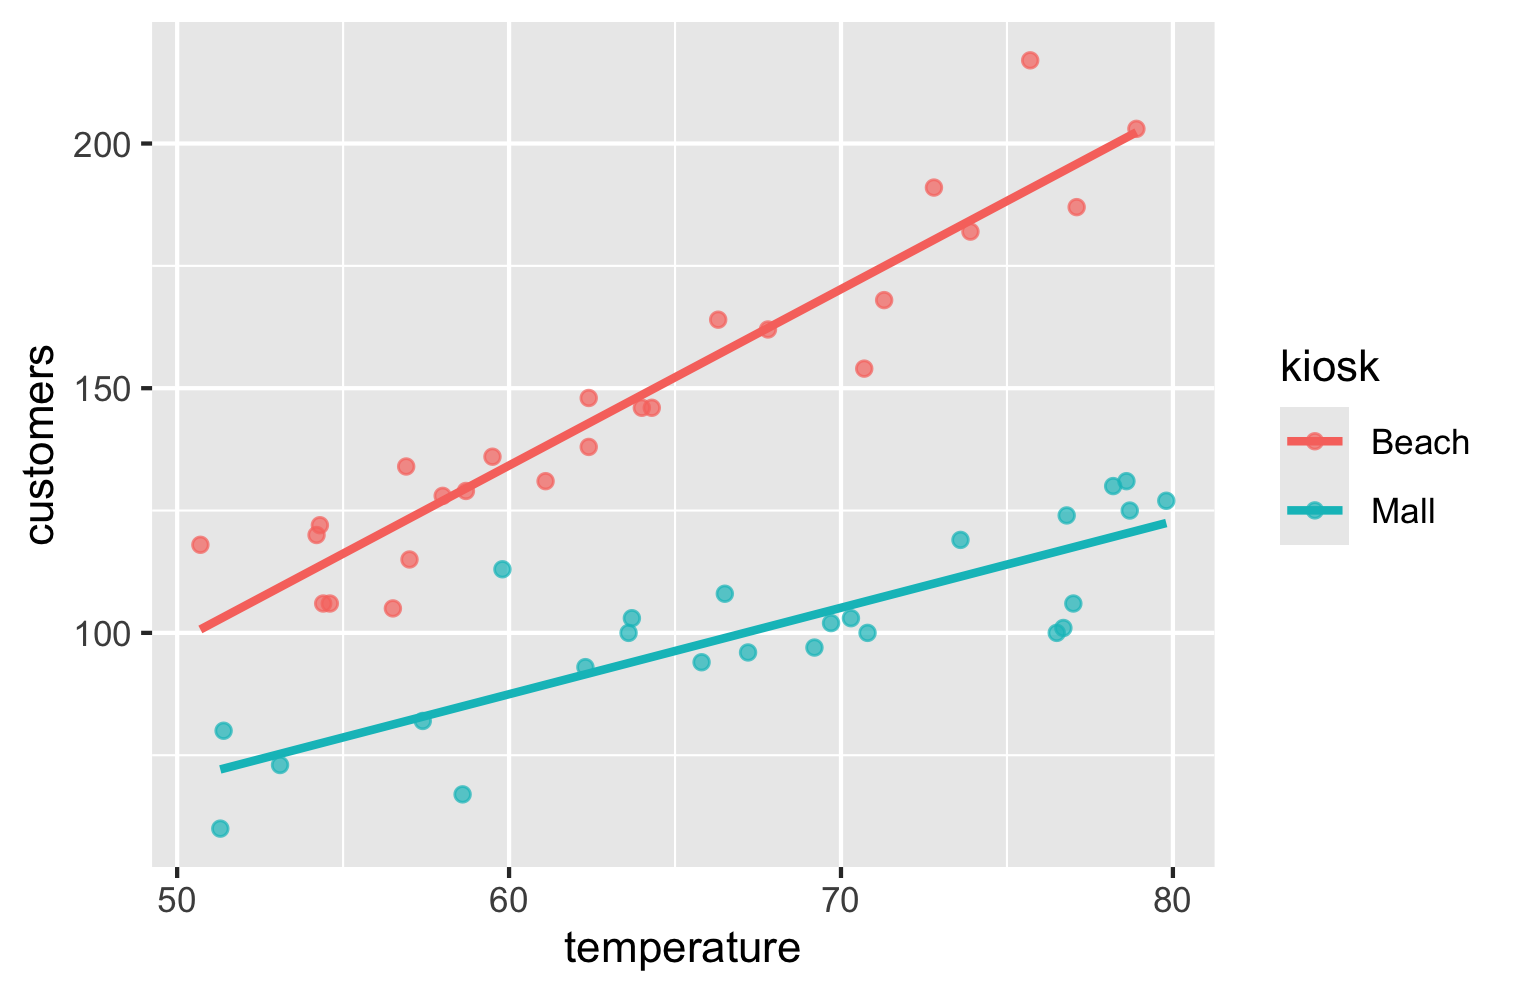
\includegraphics[width=0.7\linewidth,height=\textheight,keepaspectratio]{modules/04-more-on-models/../../images/fig-kiosk-beach-mall-kiosk-temp-lines.png}

}

\caption{\label{fig-kiosk-beach-mall-kiosk-temp-lines}Separate
least-square lines for the two kiosks showing that the beach kiosk is
more sensitive to temperature}

\end{figure}%

David looks at Figure~\ref{fig-kiosk-beach-mall-kiosk-temp-lines} and
says ``Amanda's instinct that the two kiosks relate quite differently
seems correct. The beach kiosk seems somewhat more sensitive to
temperature. Per degree increase in temperature, it gets more
incremental customers.''

Steve says ``Yeah. At lower temperatures the differences in the number
of customers between the beach kiosk and the mall kiosk are smaller, but
when it gets warmer, more people seem to want to hit the beach than the
mall. Makes perfect sense to me!''

The team feels happy that they can explain the common sense behind the
model.

Peter then writes the code to get separate models for the two kiosks.
First for the Mall kiosk.

\begin{lstlisting}[language=R]
kiosk_beach_mall_temp |> 
  filter(kiosk == "Mall") |> 
  model_train(customers ~ temperature) |> 
  coef()
\end{lstlisting}

From the output, they reconstructed the model for the Mall kiosk as:

\begin{equation}\phantomsection\label{eq-kiosk-cust-temp-mall}{
\widehat{\text{customers}} = -18.53 +  1.77\times\text{temperature} 
}\end{equation}

\begin{lstlisting}[language=R]
kiosk_beach_mall_temp |> 
  filter(kiosk == "Beach") |> 
  model_train(customers ~ temperature) |> 
  coef()
\end{lstlisting}

From the output, they reconstruct the model for the Beach kiosk as:

\begin{equation}\phantomsection\label{eq-kiosk-cust-temp-beach}{
\widehat{\text{customers}} = -82 +  3.6\times \text{temperature} 
}\end{equation}

From Figure~\ref{fig-kiosk-beach-mall-kiosk-temp-lines}, it seemed clear
that the two kiosks were quite different in how they related tgo
temperature and therefore two separate models seemed to make sense.

Suzie wonders ``Why is there such a big difference in the intercept for
these two models, -18 vs.~-82? The lines look sufficiently close!''

Peter clarifies. ``Suzie, these are \emph{intercepts}. These are the
points where the lines meet the y-axis when x = 0. In the plot, we are
seeing the x-axis starting from 50 because that is the lowest
temperature in our data. If we zoomed out to where we could see points
where the lines intersect the y axis then we would see the
correspondence between the coefficients and the plot.'' He then showed
Figure~\ref{fig-plot-showing-negative-intercepts}.

\begin{figure}

\centering{

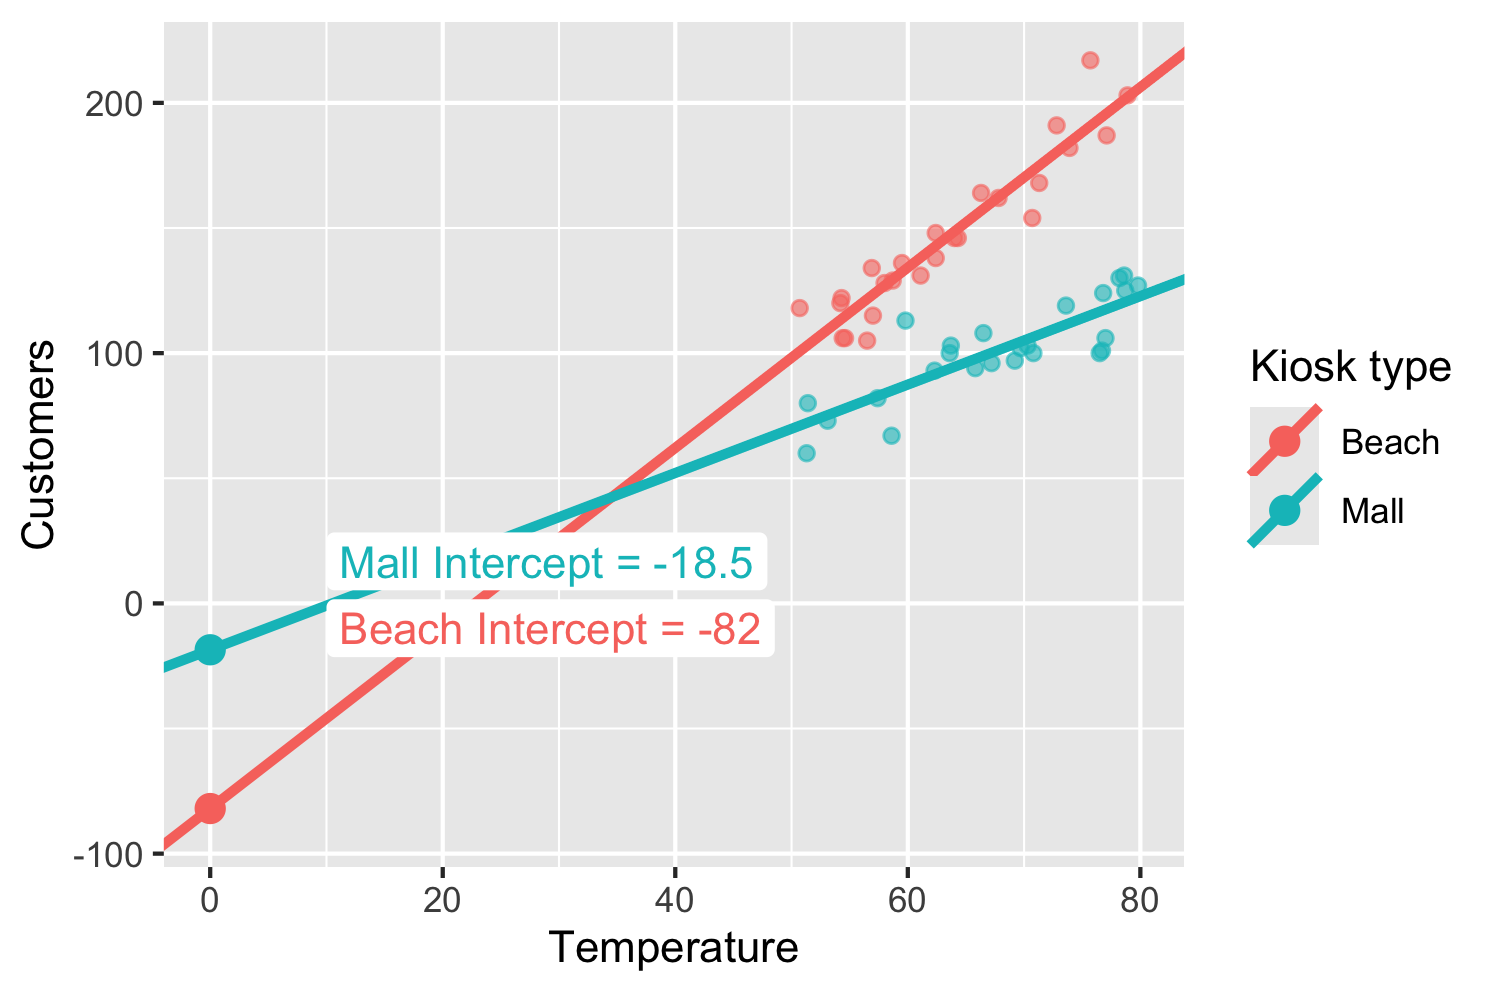
\includegraphics[width=0.7\linewidth,height=\textheight,keepaspectratio]{modules/04-more-on-models/../../images/fig-plot-showing-negative-intercepts.png}

}

\caption{\label{fig-plot-showing-negative-intercepts}Caption}

\end{figure}%

The group nods in understanding and seems relieved to see the connection
between the plot and the coefficients.

\begin{tcolorbox}[enhanced jigsaw, colback=white, leftrule=.75mm, toprule=.15mm, bottomtitle=1mm, breakable, coltitle=black, toptitle=1mm, title=\textcolor{quarto-callout-important-color}{\faExclamation}\hspace{0.5em}{Important}, opacitybacktitle=0.6, colbacktitle=quarto-callout-important-color!10!white, arc=.35mm, left=2mm, colframe=quarto-callout-important-color-frame, titlerule=0mm, rightrule=.15mm, bottomrule=.15mm, opacityback=0]

The intercept of a line is the estimated number of customers at 0°F for
the corresponding kiosk.

It's outside the observed data range, but the model still defines it.

It seems nonsensical to have negative model estimates, but if we
restrict the model to straight lines (or be linear in genera), we should
expect this.

We should use models only within the range of data that were used to
build them. In this scenario, we should not use these models outside the
range of 50°F and 80°F. If we adhere to this, then we will not generate
absurd model estimates.

\end{tcolorbox}

Later that week, they meet with Amanda again, a little fearful that they
did not stick to her \emph{simple} requirement and were giving two
different models. They tell her honestly that they had heard about a
more advanced approach that would fit both into a single model, but that
they were not sufficiently knowledgeable to present it. They also tell
her that the results would still be the same as with two separate
models.

Fortunately, Amanda seems happy with their work. But she said that she
would prefer a single simple model rather than two, even if it meant
somewhat lower quality estimates.

The team's spirits sank.

But Suzie was ready. She said, ``I too have Dr.~Berlinsky for a class
and, just before leaving campus for this meeting. I was worried about
our model being a bit more complex than what Amanda wanted.

Dr.~B said, and as we already know too, that temperature affects the two
kiosks differently. The line for the beach kiosk is steeper, and our two
separate models capture that difference.

However, he also said that, in real life, simpler models also have their
virtues. Even if the more complex model gives slightly better results,
its complexity might add costs in terms of overloading the operating
personnel a bit, which has its costs too. If a simpler solution gave
close results then, on balance it might be alright.

He said that we could build a simpler model that assumes that the
temperature affects both kiosks equally (same slope). That model looks
like this.'' And she showed Figure~\ref{fig-no-interaction-kiosk-model}.

\begin{figure}

\centering{

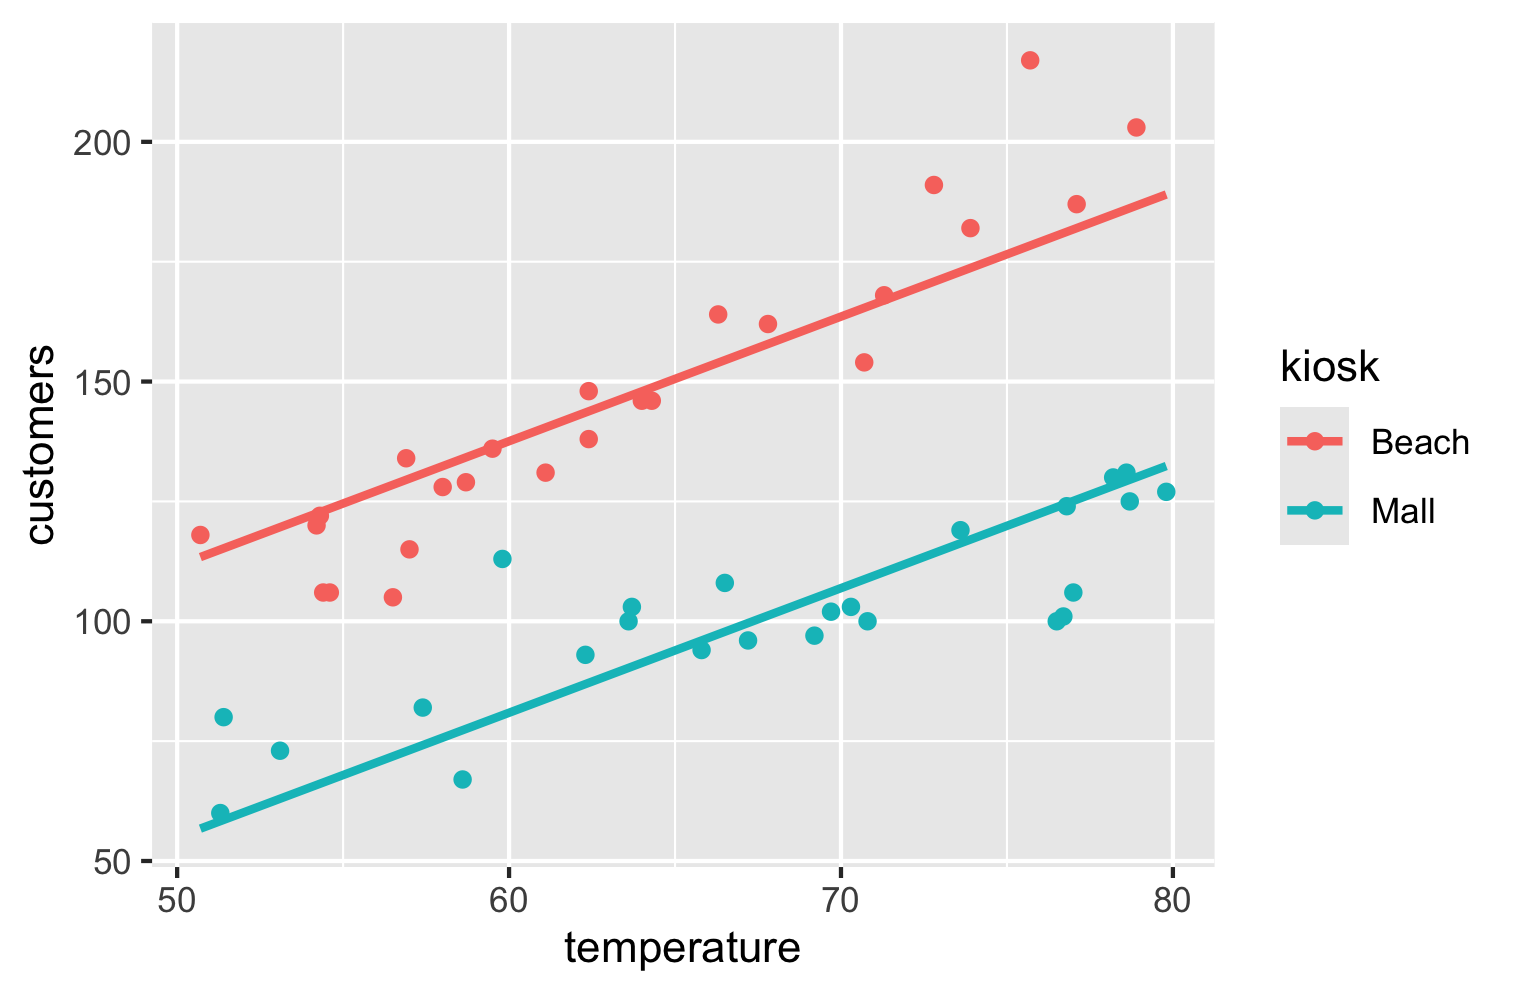
\includegraphics[width=0.7\linewidth,height=\textheight,keepaspectratio]{modules/04-more-on-models/../../images/fig-no-interaction-kiosk-model.png}

}

\caption{\label{fig-no-interaction-kiosk-model}Kiosk model with no
interaction effect}

\end{figure}%

Suzie then showed the R code to get the model equation for this.

\begin{lstlisting}[language=R]
kiosk_beach_mall_temp |> 
  model_train(customers ~ temperature + kiosk) |> 
  coef()
\end{lstlisting}

\begin{lstlisting}
(Intercept) temperature   kioskMall 
      -18.4         2.6       -56.6 
\end{lstlisting}

They reconstruct the model equation
Equation~\ref{eq-kiosk-mode-no-intxn} from the output.

\begin{equation}\phantomsection\label{eq-kiosk-mode-no-intxn}{
\widehat{\text{customers}} = -18.4 + 2.6\times \text{temperature} +
\begin{cases}
0 & \text{if } \text{kiosk} = \text{"Beach"} \\
-57 &\text{if } \text{kiosk} = \text{"Mall"}
\end{cases}
}\end{equation}

Amanda says ``Now you're talking. I prefer this one. I do not want to
complicate things too much.''

The team resolved to learn more about the \emph{interaction effects}
that Dr.~Berlinsky had spoken about and present that to Amanda when
possible.

Dr.~Berlinsky had also said that there is a whole field called
\emph{Machine Learning} that would enable them to build models that went
beyond their linear ones and give better estimates. They saw that their
school offered an elective course titled ``Business Applications of
Machine Learning'' and decided that they would take it as a group as
they worked on more projects with Amanda.

\part{Explanatory Power of a Model}

\chapter*{Module 5: Explanatory Power of a
Model}\label{module-5-explanatory-power-of-a-model}
\addcontentsline{toc}{chapter}{Module 5: Explanatory Power of a Model}

\markboth{Module 5: Explanatory Power of a Model}{Module 5: Explanatory
Power of a Model}

In prior modules you have learned about models, to visualize them and to
express models as functions. In this module you will learn how to assess
the quality of models as measured by its \emph{explanatory power}.

\section*{Learning Goals}\label{learning-goals-4}
\addcontentsline{toc}{section}{Learning Goals}

\markright{Learning Goals}

\begin{itemize}
\tightlist
\item
  a
\item
  b
\item
  c
\end{itemize}

\section*{Structure of This Module}\label{structure-of-this-module-4}
\addcontentsline{toc}{section}{Structure of This Module}

\markright{Structure of This Module}

\begin{itemize}
\tightlist
\item
  a
\item
  b
\item
  c
\end{itemize}

\chapter{\texorpdfstring{\emph{Explain} as used in
Statistics}{Explain as used in Statistics}}\label{explain-as-used-in-statistics}

To assess the quality of a model, we talk about its \emph{explanatory
power}. Statistics uses the term \emph{explain} in a very specific way
and you will need to understand it to truly grasp how we measure the
quality of statistical models in the next few chapters. In this chapter
we focus only on the term \emph{explain} as used in statistics.

\section{Relationships Between Variables
Revisited}\label{relationships-between-variables-revisited}

In Chapter~\ref{sec-visualizing-relationships} we saw what it means for
two variables to be related to each other. We also saw that
relationships can be positive or negative, strong or weak.

When we say that two variables are related, we mean that knowing the
value of one variable helps us predict the value of the other variable.
For example, if we know that a person has a high income, we can predict
that they are \emph{likely} to spend more on dining out than someone
with a low income.

If we are given the weights of several people and see that they are all
around 150 pounds, we can predict that their heights are likely to be
around 5'7'' to 5'10''. However, if we know that one person weighs 150
pounds and another person weighs 300 pounds, we can predict that the
second person is likely to be taller than the first person.

Of course, there is no guarantee that every person who weighs around 150
pounds is between 5'7'' and 5'10''. There will be exceptions. But in
general, knowing the weight of a person helps us make better predictions
about their height than without this information. Similarly, there is no
guarantee that wevery person who weighs 300 pounds is taller than every
person who weighs 150 pounds. But in general, knowing that a person
weighs 300 pounds helps us make better predictions about their height
relative to someone who weighs 150 pounds.

In general, when two variables are related, knowing the value of one
variable helps us make better predictions about the value of the other
variable.

Figure~\ref{fig-advertising-sales-channel-1a} shows the relationship
between advertising expenses and weekly sales for a company (based on
the data frame \emph{advertising\_sales\_channel}). As advertising
expenses increase, weekly sales also tend to increase. If we know that
the company is going to spend \$80k during a particular week, we can
expect that the sales will likely be between around 200 to 300k units.
If we know that the company is going to spend only \$20k during a
particular week, we can expect that the sales will likely be between
around 100 to 200k units.

\begin{figure}

\centering{

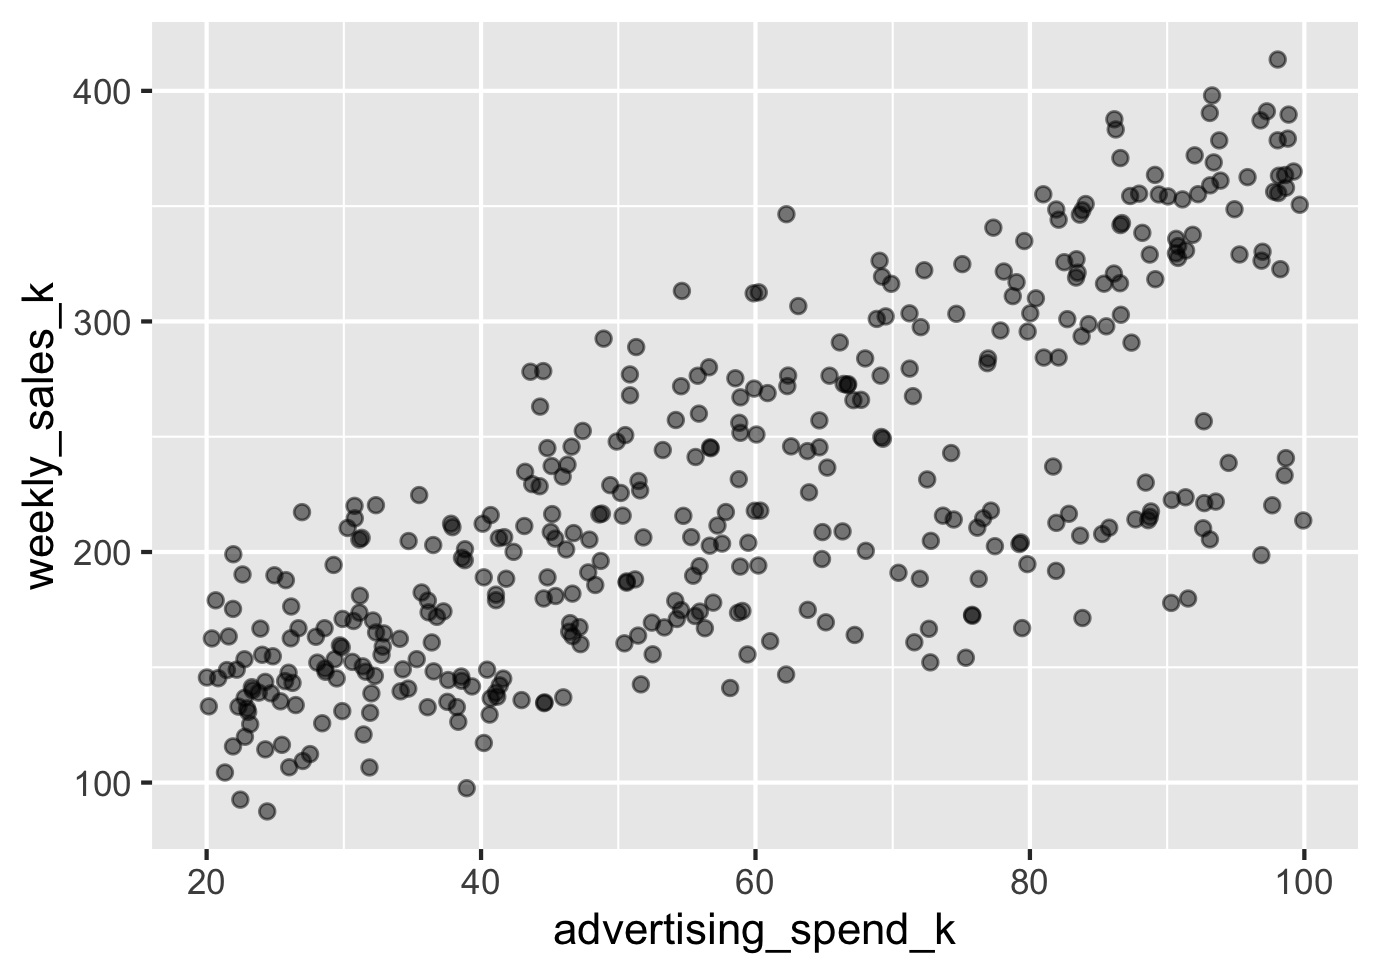
\includegraphics[width=0.7\linewidth,height=\textheight,keepaspectratio]{modules/05-explanatory-power-of-models/../../images/fig-advertising-sales-channel-1.png}

}

\caption{\label{fig-advertising-sales-channel-1a}Relationship between
advertising expenses and weekly sales}

\end{figure}%

Relationships between variables play a very important role in statistics
and pave the path for us to \emph{explain} things statistically

\section{Explaining One Variable with
Another}\label{explaining-one-variable-with-another}

Suppose we see data about the selling prices of homes in a certain
neighborhood. AT first we see only the prices and nothing else. We see
variability in the prices. Some homes are priced low, some are priced
high, and many are priced in between. We might wonder why there is such
variability in the prices, even though the homes are all in the same
neighborhood.

Then we get more information about the homes, such as their sizes (in
square feet). We might then see that the home sizes also vary. Some
homes are small, some are large, and many are in between. We might then
wonder if the variability in home sizes is related to the variability in
home prices. If we find that larger homes tend to be priced higher and
smaller homes tend to be priced lower, we can say ``Aha, that
\emph{explains} it. I see now why some homes are priced higher and some
are priced lower. It's because of their sizes.''

In statistics, when we say that one variable \emph{explains} another
variable, we mean that knowing the value of the first variable helps us
make better predictions about the value of the second variable. In the
example above, knowing the size of a home helps us make better
predictions about its price. Therefore, we say that home size
\emph{explains} home price.

When we say that one variable \emph{explains} another variable, we are
not saying that the first variable is the \emph{cause} of the second
variable. We are only saying that knowing the value of the first
variable helps us make better predictions about the value of the second
variable. In the example above, we are not saying that home size
\emph{causes} home price. We are only saying that knowing the size of a
home helps us make better predictions about its price. There could be
other factors at play that also affect home prices, such as location,
age of the home, and so on.

Relationships between variables helps to reduce uncertainty about the
value of one variable when we know the value of a related variable.

For example, suppose we have the same list of prices of homes in a
neighborhood. I choose one house at random from the list and and ask you
to guess the price of that home. Without any other information, you
might guess the average price of homes in that neighborhood (based on
what you learned in Chapter~\ref{sec-mean-model}).

I then give you a hint about the size of the home (in sqft) that I
randomly picked. If you know the relationship between these two
variables \emph{price} and \emph{size} then you can make a better guess
about the price than just the overall average.

When two variables are related, the variability in the values of one
variable \emph{explain} the variability in the values of the other. Why
do home prices vary? Because home sizes vary. Why do sales vary? Because
advertising expenses vary. Why do weights vary? Because heights vary.
And so on.

In statistics, we often use one variable to \emph{explain} another
variable. The variable that is used to explain is called the
\emph{explanatory variable} (or sometimes the \emph{independent
variable}). The variable that is being explained is called the
\emph{outcome variable}, \emph{response variable} (or sometimes the
\emph{dependent variable}).

\begin{tcolorbox}[enhanced jigsaw, colback=white, leftrule=.75mm, toprule=.15mm, bottomtitle=1mm, breakable, coltitle=black, toptitle=1mm, title={Quick Check}, opacitybacktitle=0.6, colbacktitle=quarto-callout-note-color!10!white, arc=.35mm, left=2mm, colframe=quarto-callout-note-color-frame, titlerule=0mm, rightrule=.15mm, bottomrule=.15mm, opacityback=0]

Suppose I have two variables \emph{a} and \emph{b} and these two are
strongly positively related. Suppose also that I have the ability to
control the values of \emph{a} (for example, it might be the amount of
money I spend on advertising, or the price, or the number of employees I
allocate to a project). I want higher values of \emph{b}. Can I just
increase \emph{a} to achieve my goal?

\end{tcolorbox}

\begin{tcolorbox}[enhanced jigsaw, colback=white, leftrule=.75mm, toprule=.15mm, bottomtitle=1mm, breakable, coltitle=black, toptitle=1mm, title={Suggested answer}, opacitybacktitle=0.6, colbacktitle=quarto-callout-note-color!10!white, arc=.35mm, left=2mm, colframe=quarto-callout-note-color-frame, titlerule=0mm, rightrule=.15mm, bottomrule=.15mm, opacityback=0]

Maybe, maybe not. Just because two variables are related does not mean
that changing one variable will \emph{cause} the other variable to
change. There could be other factors at play that affect \emph{b}. For
example, if \emph{a} is advertising expense and \emph{b} is sales,
increasing advertising expenses might lead to higher sales, but it also
might not if the market is saturated or if there are other issues
affecting sales. Therefore, while knowing that \emph{a} and \emph{b} are
related helps us make better predictions about \emph{b} when we know
\emph{a}, it does not guarantee that changing \emph{a} will change
\emph{b}. Also, there is always the possibility that \emph{b} is causing
\emph{a}, or that some other variables are causing both \emph{a} and
\emph{b} to change.

The general rule is: Correlation does not imply causation.

\end{tcolorbox}

\begin{tcolorbox}[enhanced jigsaw, colback=white, leftrule=.75mm, toprule=.15mm, bottomtitle=1mm, breakable, coltitle=black, toptitle=1mm, title=\textcolor{quarto-callout-warning-color}{\faExclamationTriangle}\hspace{0.5em}{Warning}, opacitybacktitle=0.6, colbacktitle=quarto-callout-warning-color!10!white, arc=.35mm, left=2mm, colframe=quarto-callout-warning-color-frame, titlerule=0mm, rightrule=.15mm, bottomrule=.15mm, opacityback=0]

The above does not mean that correlation indicates the absence of
causation. In many cases, there is indeed a causal relationship between
two variables that are correlated. However, correlation alone is not
sufficient to establish causation. Additional evidence and analysis are
needed to determine whether a causal relationship exists.

\end{tcolorbox}

\section{Model as an Explainer of variation in outcome
variable}\label{model-as-an-explainer-of-variation-in-outcome-variable}

We spoke earlier about a variable being an explainer. In statistics, we
also talk about a model as \emph{explaining} the variation in its
outcome variable. When we say that a model \emph{explains} the outcome
variable, we mean that the explanatory variables used in the model
combined with the model coefficients help us make better predictions
about the outcome variable, or to explain a phenomenon.

For example, suppose a researcher is interested in the effect of study
time and attendance on exam scores. We are not using the term here
\emph{effect} in the sense of cause and effect, but more loosely in the
sense of relationship.

The researcher collects data on students' study time, attendance, and
exam scores. The researcher then fits a statistical model with study
time and attendance as explanatory variables and exam score as the
outcome variable. If the model results of student performance closely
match reality, then we can conclude that the model has explained a
real-world phenomenon: that students who study more and attend classes
more regularly tend to perform better on exams. In this case, we can say
that the model comprising study time and class attendance
\emph{explains} the variability in exam scores.

\begin{tcolorbox}[enhanced jigsaw, colback=white, leftrule=.75mm, toprule=.15mm, bottomtitle=1mm, breakable, coltitle=black, toptitle=1mm, title=\textcolor{quarto-callout-important-color}{\faExclamation}\hspace{0.5em}{Important}, opacitybacktitle=0.6, colbacktitle=quarto-callout-important-color!10!white, arc=.35mm, left=2mm, colframe=quarto-callout-important-color-frame, titlerule=0mm, rightrule=.15mm, bottomrule=.15mm, opacityback=0]

Once again, we cannot infer any causality here based solely on this
model. It could very well be that students who are more motivated to do
well on exams also tend to study more and attend classes more regularly.
The model simply helps us understand the relationships between these
variables and make better predictions about exam scores based on study
time and attendance. To establish causality, we would need to conduct
controlled experiments or use other methods to rule out confounding
factors.

\end{tcolorbox}

\begin{tcolorbox}[enhanced jigsaw, colback=white, leftrule=.75mm, toprule=.15mm, bottomtitle=1mm, breakable, coltitle=black, toptitle=1mm, title={Quick Check}, opacitybacktitle=0.6, colbacktitle=quarto-callout-note-color!10!white, arc=.35mm, left=2mm, colframe=quarto-callout-note-color-frame, titlerule=0mm, rightrule=.15mm, bottomrule=.15mm, opacityback=0]

Choose any two disciplines of business (e.g., marketing, finance,
manufacturing, accounting, \ldots) and give an example of one variable
\emph{explaning} another.

\end{tcolorbox}

\begin{tcolorbox}[enhanced jigsaw, colback=white, leftrule=.75mm, toprule=.15mm, bottomtitle=1mm, breakable, coltitle=black, toptitle=1mm, title={Suggested answer}, opacitybacktitle=0.6, colbacktitle=quarto-callout-note-color!10!white, arc=.35mm, left=2mm, colframe=quarto-callout-note-color-frame, titlerule=0mm, rightrule=.15mm, bottomrule=.15mm, opacityback=0]

Marketing example: Advertising expenses \emph{explain} sales. Knowing
how much a company spends on advertising helps us make better
predictions about its sales.

Finance example: Credit score \emph{explains} loan default risk. Knowing
a borrower's credit score helps us make better predictions about the
likelihood of them defaulting on a loan.

Manufacturing example: Machine maintenance frequency \emph{explains}
production downtime. Knowing how often machines are maintained helps us
make better predictions about the amount of downtime in production.

Accounting example: Revenue \emph{explains} profit. Knowing a company's
revenue helps us make better predictions about its profit.

Each of the examples can go the other way as well. For example, sales
can also \emph{explain} advertising expenses, loan default risk can also
\emph{explain} credit score, and so on. The key point is that when two
variables are related, knowing the value of one variable helps us make
better predictions about the value of the other variable.

\end{tcolorbox}

\begin{tcolorbox}[enhanced jigsaw, colback=white, leftrule=.75mm, toprule=.15mm, bottomtitle=1mm, breakable, coltitle=black, toptitle=1mm, title={Quick Check}, opacitybacktitle=0.6, colbacktitle=quarto-callout-note-color!10!white, arc=.35mm, left=2mm, colframe=quarto-callout-note-color-frame, titlerule=0mm, rightrule=.15mm, bottomrule=.15mm, opacityback=0]

Choose any two disciplines of business (e.g., marketing, finance,
manufacturing, accounting, \ldots) and give an example of one variable
that generally does not \emph{explan} another.

\end{tcolorbox}

\begin{tcolorbox}[enhanced jigsaw, colback=white, leftrule=.75mm, toprule=.15mm, bottomtitle=1mm, breakable, coltitle=black, toptitle=1mm, title={Suggested answer}, opacitybacktitle=0.6, colbacktitle=quarto-callout-note-color!10!white, arc=.35mm, left=2mm, colframe=quarto-callout-note-color-frame, titlerule=0mm, rightrule=.15mm, bottomrule=.15mm, opacityback=0]

Marketing example: Customer satisfaction score does not generally
\emph{explain} the number of employees in a company. Knowing the
customer satisfaction score does not help us make better predictions
about the number of employees.

Finance example: A company's stock price does not generally explain the
latitude of its headquarters. Knowing the stock price does not help us
make better predictions about how far north or south the company is
located.

Manufacturing example: Production volume does not generally
\emph{explain} the color of the factory building. Knowing the production
volume does not help us make better predictions about the color of the
building.

Accounting example: Check number does not generally \emph{explain} the
check amount. Knowing the check number does not help us make better
predictions about the amount of the check.

\end{tcolorbox}

\begin{tcolorbox}[enhanced jigsaw, colback=white, leftrule=.75mm, toprule=.15mm, bottomtitle=1mm, breakable, coltitle=black, toptitle=1mm, title=\textcolor{quarto-callout-important-color}{\faExclamation}\hspace{0.5em}{Important}, opacitybacktitle=0.6, colbacktitle=quarto-callout-important-color!10!white, arc=.35mm, left=2mm, colframe=quarto-callout-important-color-frame, titlerule=0mm, rightrule=.15mm, bottomrule=.15mm, opacityback=0]

We said that a variable can explain another variable. Let us be more
specific as a preparation for the next few chapters.

If you go back to the house prices example, we said that we initially
wonder why house prices vary and then realize looking at the sqft of the
houses that the sqft varies and therefore naturally the prices vary
because sqft and price are related.

Another important way to phrase this is to say that the variability in
sqft \emph{explains} the variability in price. We will soon be using the
act=ual variance of the prices as one important piece in the puzzle of
measuring the explanatory power of a model.

\emph{Variance} is going to start playing an important role. As I have
said before, statistics is all about measuring and managing variability.

\end{tcolorbox}

\chapter{Using Models to Explain Variation in Outcome
Variables}\label{sec-explaining-variation}

In the previous chapter, we learned how to compute \textbf{model
estimates} and \textbf{residuals}. For each day, the model gave us an
estimated number of customers, and the residual told us how far off that
prediction was from reality.

Amanda asked the interns to come over to the the mall kiosk so that they
could get a feel for the actual operation while they discussed how to
take this project forward. She seemed a bit concerned.

``You have helped us improve efficiency over the past few months. I have
been able to maintain stable staffing levels while not over-staffing on
slow days, or under-staffing on busy days.

I have seen that using data properly does indeed help me to make better
decisions and am planning to sign up for a service that will give me
more data about our operations \ldots{} but they are pricey and I don't
want to spend the money without knowing how much potential we have to
improve our models. I want to know how much room we have to improve. So
my first question for you all is:

\begin{quote}
\emph{How good is this model, really? Do we have room to improve? Or
have we hit the ceiling?}
\end{quote}

Well, that was three questions \ldots'' Amanda said with a smile. ``Why
don't you discuss and we can talk about it after a while?''

\begin{figure}

\centering{

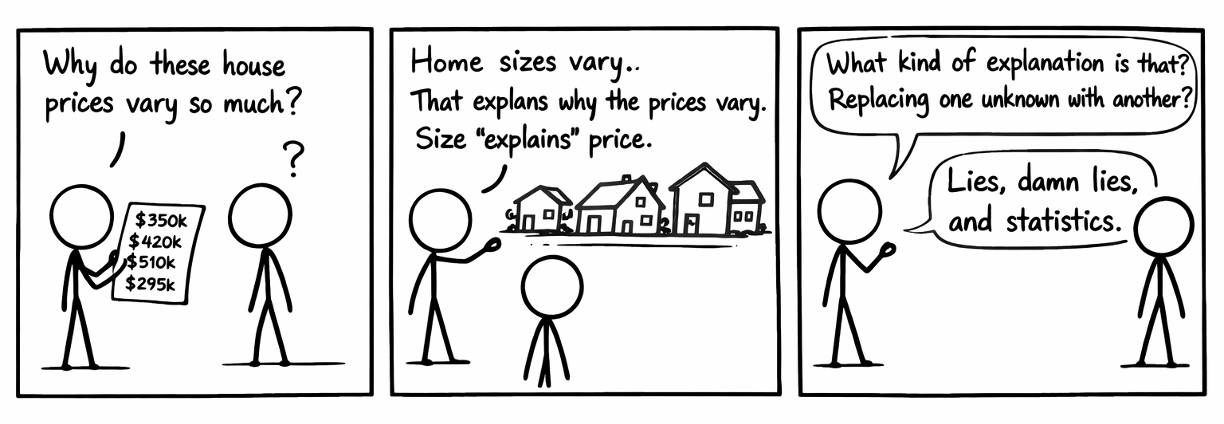
\includegraphics[width=0.7\linewidth,height=\textheight,keepaspectratio]{modules/05-explanatory-power-of-models/../../images/fig-explain-1.png}

}

\caption{\label{fig-explain-1}Explaining variation?}

\end{figure}%

\begin{figure}

\centering{

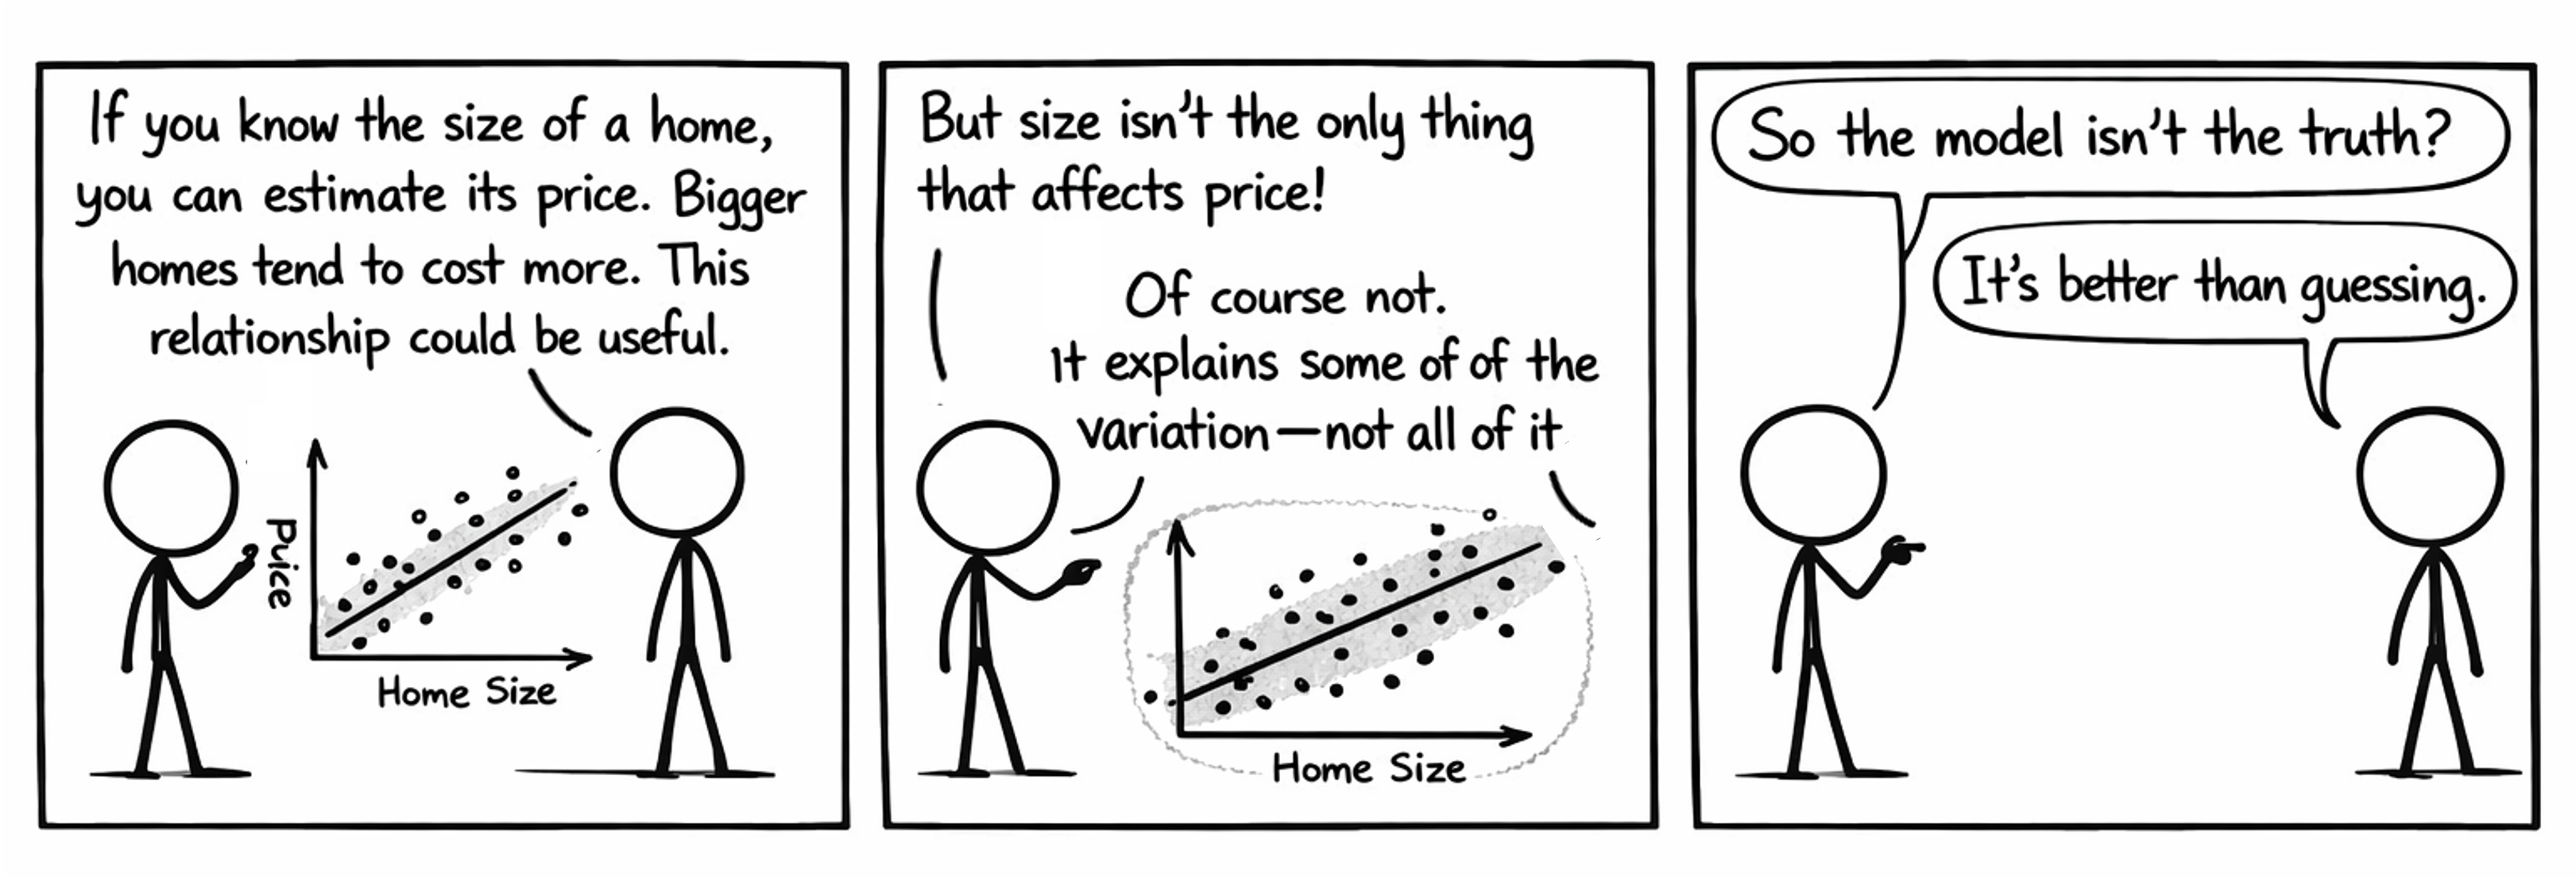
\includegraphics[width=0.7\linewidth,height=\textheight,keepaspectratio]{modules/05-explanatory-power-of-models/../../images/fig-explain-2.png}

}

\caption{\label{fig-explain-2}When two variables are related, knowing
the value of one can reduce uncertainty in the other \ldots{} to some
extent}

\end{figure}%

The interns are about to discover an important concept in linear models
(the kind we build in this course) -- \textbf{variance of the outcome
variable is split between what the model explains and what it does not}.

\section{Model as an explainer of variation in the outcome
variable}\label{model-as-an-explainer-of-variation-in-the-outcome-variable}

Steve began ``To map back to what we did in our last few months for
Amanda, we might say that when look at the outcome variable -- the
number of customers each day -- and see the variability. Initially when
Amanda just gave us the numbers of customers alone, we could not do much
and suggested that the best she could do was to use the average as the
estimate each day for both kiosks.

Some of the variability in the number of customers arises because of
their location. The beach kiosk has its pattern and the mall one has its
quirks. For example, on average the beach kiosk saw 40 more customers
each day. So using the same staffing level for both kiosks does not make
sense.

So, one reason for the variation in the numbers was the kiosk each
number was associated with. Once Amanda gave us the kiosk for each
number in the data, we were hen able to give her a separate estimate for
each kiosk and she confirmed that it improved matters for her.''

\begin{tcolorbox}[enhanced jigsaw, colback=white, leftrule=.75mm, toprule=.15mm, bottomtitle=1mm, breakable, coltitle=black, toptitle=1mm, title=\textcolor{quarto-callout-important-color}{\faExclamation}\hspace{0.5em}{Important}, opacitybacktitle=0.6, colbacktitle=quarto-callout-important-color!10!white, arc=.35mm, left=2mm, colframe=quarto-callout-important-color-frame, titlerule=0mm, rightrule=.15mm, bottomrule=.15mm, opacityback=0]

The model that used kiosk as the explanatory variable explained, or
clarified, why there was some variability in the number of customers
overall, but it did not explain all of the variability. For example, we
know that the overall average number of customers was around 120 while
the average for the mall was around 100 and for the beach was around
140. So if we look at the sales for a given day and see that it is 150,
we can be pretty sure (but not 100\% certain) that this sale likely was
for the beach kiosk. So, in this sense, the kiosk location ``explains''
the number of customers.

\end{tcolorbox}

Angela joined in: ``But, there is still variability in the sales for
each kiosk. That is, not all the numbers for the beach kiosk are the
same, no=r are the numbers for the mall kiosk the same. So just knowing
the kiosk location did not tell us the whole story. We still had some
more variability to explain. We added temperature and that improved
matters for Amanda.''

\begin{tcolorbox}[enhanced jigsaw, colback=white, leftrule=.75mm, toprule=.15mm, bottomtitle=1mm, breakable, coltitle=black, toptitle=1mm, title=\textcolor{quarto-callout-important-color}{\faExclamation}\hspace{0.5em}{Important}, opacitybacktitle=0.6, colbacktitle=quarto-callout-important-color!10!white, arc=.35mm, left=2mm, colframe=quarto-callout-important-color-frame, titlerule=0mm, rightrule=.15mm, bottomrule=.15mm, opacityback=0]

We know that the average number of customers for the beach kiosk is
close to 140 and that temperature has a role to play in the number of
customers.

Let us say in the data we see 150 customers (above average) for a given
day at the beach kiosk. WHat does that say about the likely temperature
on that day? It would be reasonable to expect that the temperature was
also above average on that day -- of course we cannot be 100\% sure, but
that would be a reasonable expectation. In this sense the model with
kiosk and temperature as explanatory variables ``explains'' the number
of customers.

\end{tcolorbox}

Igor and Dave almost simultaneously say ``What if together the kiosk
location and the temperature tell us everything we need to know. What if
they explain all the variability in the number of customers?''

Suzie immediately says ``That would mean that the model with kiosk
location and temperature gives estimates that match actual values
\emph{exactly}! Does it?''

Peter brings up a table showing the original data and the model
estimates (tbl-temp-kiosk-model-estimates) using the following code.

\begin{lstlisting}[language=R]
  kiosk_beach_mall_temp |> 
    mutate(mod_est = model_values(customers ~ temperature + kiosk))
\end{lstlisting}

\begin{longtable}[]{@{}lrlrr@{}}
\caption{Kiosk data and model estimates for customers \textasciitilde{}
temperature + kiosk (model estimates
rounded)\{\#tbl-temp-kiosk-model-estimates\}}\tabularnewline
\toprule\noalign{}
day & customers & kiosk & temperature & mod\_est \\
\midrule\noalign{}
\endfirsthead
\toprule\noalign{}
day & customers & kiosk & temperature & mod\_est \\
\midrule\noalign{}
\endhead
\bottomrule\noalign{}
\endlastfoot
D01 & 67 & Mall & 58.6 & 77 \\
D02 & 119 & Mall & 73.6 & 116 \\
D03 & 93 & Mall & 62.3 & 87 \\
D04 & 100 & Mall & 76.5 & 124 \\
D05 & 130 & Mall & 78.2 & 128 \\
D06 & 80 & Mall & 51.4 & 59 \\
D07 & 94 & Mall & 65.8 & 96 \\
D08 & 124 & Mall & 76.8 & 125 \\
D09 & 108 & Mall & 66.5 & 98 \\
D10 & 103 & Mall & 63.7 & 91 \\
D11 & 125 & Mall & 78.7 & 130 \\
D12 & 100 & Mall & 63.6 & 90 \\
D13 & 103 & Mall & 70.3 & 108 \\
D14 & 96 & Mall & 67.2 & 100 \\
D15 & 73 & Mall & 53.1 & 63 \\
D16 & 106 & Mall & 77.0 & 125 \\
D17 & 82 & Mall & 57.4 & 74 \\
D18 & 60 & Mall & 51.3 & 58 \\
D19 & 113 & Mall & 59.8 & 80 \\
D20 & 131 & Mall & 78.6 & 129 \\
D21 & 101 & Mall & 76.7 & 124 \\
D22 & 100 & Mall & 70.8 & 109 \\
D23 & 97 & Mall & 69.2 & 105 \\
D24 & 127 & Mall & 79.8 & 132 \\
D25 & 102 & Mall & 69.7 & 106 \\
D01 & 168 & Beach & 71.3 & 167 \\
D02 & 164 & Beach & 66.3 & 154 \\
D03 & 162 & Beach & 67.8 & 158 \\
D04 & 129 & Beach & 58.7 & 134 \\
D05 & 106 & Beach & 54.4 & 123 \\
D06 & 203 & Beach & 78.9 & 187 \\
D07 & 187 & Beach & 77.1 & 182 \\
D08 & 154 & Beach & 70.7 & 165 \\
D09 & 182 & Beach & 73.9 & 174 \\
D10 & 118 & Beach & 50.7 & 113 \\
D11 & 146 & Beach & 64.3 & 149 \\
D12 & 191 & Beach & 72.8 & 171 \\
D13 & 105 & Beach & 56.5 & 128 \\
D14 & 136 & Beach & 59.5 & 136 \\
D15 & 134 & Beach & 56.9 & 130 \\
D16 & 122 & Beach & 54.3 & 123 \\
D17 & 148 & Beach & 62.4 & 144 \\
D18 & 138 & Beach & 62.4 & 144 \\
D19 & 131 & Beach & 61.1 & 140 \\
D20 & 106 & Beach & 54.6 & 124 \\
D21 & 120 & Beach & 54.2 & 122 \\
D22 & 115 & Beach & 57.0 & 130 \\
D23 & 146 & Beach & 64.0 & 148 \\
D24 & 128 & Beach & 58.0 & 132 \\
D25 & 217 & Beach & 75.7 & 178 \\
\end{longtable}

Angela says ``Darn. The predictions look reasonably close, but they are
nowhere near exact. So the model is \emph{not perfect}. How can we
improve it?''

Igor says ``Guys, I think I understand this a bit better now. It makes
sense that we cannot estimate the exact number of customers just using
the temperature and kiosk location. After all, the real world is more
complex than that. Many other factors can and do affect the number of
customers.''

Dave says ``Yes, the other day I was at the beach on a nice warm day and
yet I only saw a few people out on the beach. We had an important
playoff game in town. So, there you go, that is one thing that affects
the number of customers, but which is not in our model.''

Angela then says ``So it looks like we cannot improve things for Amanda
unless she gives us more data. But can we answer her question of how
good the model is? May be it is not \emph{exact}, but it might still be
good enough that she should not be spending money to get more data. I
mean the extra benefit from that information might not be worth the
cost.''

Suzie has an idea ``Let us put some hard numbers on this OK? If we are
trying to find out how much variability the model \emph{explains}. What
does that mean? I mean, how much variability is there to explain in the
first place?''

Igor lights up ``We are talking about explaining variability in the
daily number of customers. Why not just use the variance of that
variable?''

Suzie writes code immediately to calculate that:

\begin{lstlisting}[language=R]
kiosk_beach_mall_temp |> 
  summarize(cust_var = var(customers))
\end{lstlisting}

\begin{lstlisting}
# A tibble: 1 x 1
  cust_var
     <dbl>
1    1169.
\end{lstlisting}

Dave ``OK. The total variance in the number of customers is 1169. Where
do we go from here?''

Angela ``Guys, let us slow down a wee bit here. Can we please go back to
the simplest model we had, and start thinking from there? That might
help us wrap our heads around this better.''

Igor ``OK. In our simplest model, we just estimated the daily number of
customers as the average of the number of customers. We completely
ignored the kiosk location or the temperature because at that time we
did not have those variables. So how much variation does that model
explain? Can we first see the model values for each row?''

Again Suzie whips out code to add the model estimates to the data frame
and produces Table~\ref{tbl-mean-model-estimates-kiosk-1}:

\begin{lstlisting}[language=R]
kiosk_beach_mall_temp |> 
  mutate(mod_est = model_values(customers ~ 1))
\end{lstlisting}

\begin{longtable}[]{@{}rlrr@{}}
\caption{Model estimates for customers \textasciitilde{} 1, same as the
mean model
(rounded)}\label{tbl-mean-model-estimates-kiosk-1}\tabularnewline
\toprule\noalign{}
customers & kiosk & temperature & model\_est \\
\midrule\noalign{}
\endfirsthead
\toprule\noalign{}
customers & kiosk & temperature & model\_est \\
\midrule\noalign{}
\endhead
\bottomrule\noalign{}
\endlastfoot
66.78076 & Mall & 58.62733 & 124 \\
118.66666 & Mall & 73.64915 & 124 \\
93.43390 & Mall & 62.26931 & 124 \\
100.36348 & Mall & 76.49052 & 124 \\
130.40991 & Mall & 78.21402 & 124 \\
79.90381 & Mall & 51.36669 & 124 \\
93.75559 & Mall & 65.84316 & 124 \\
124.09655 & Mall & 76.77257 & 124 \\
108.27050 & Mall & 66.54305 & 124 \\
103.27566 & Mall & 63.69844 & 124 \\
124.68300 & Mall & 78.70500 & 124 \\
100.05773 & Mall & 63.60002 & 124 \\
103.27945 & Mall & 70.32712 & 124 \\
95.67201 & Mall & 67.17900 & 124 \\
73.28583 & Mall & 53.08774 & 124 \\
106.21587 & Mall & 76.99475 & 124 \\
81.82622 & Mall & 57.38263 & 124 \\
60.35403 & Mall & 51.26179 & 124 \\
112.81761 & Mall & 59.83762 & 124 \\
130.52786 & Mall & 78.63511 & 124 \\
100.83468 & Mall & 76.68618 & 124 \\
100.07004 & Mall & 70.78410 & 124 \\
96.94184 & Mall & 69.21520 & 124 \\
127.44578 & Mall & 79.82809 & 124 \\
102.03122 & Mall & 69.67117 & 124 \\
168.20985 & Beach & 71.25591 & 124 \\
163.65952 & Beach & 66.32198 & 124 \\
162.31480 & Beach & 67.82426 & 124 \\
129.13389 & Beach & 58.67479 & 124 \\
106.40419 & Beach & 54.41341 & 124 \\
203.48841 & Beach & 78.89073 & 124 \\
187.48142 & Beach & 77.06897 & 124 \\
153.84239 & Beach & 70.72116 & 124 \\
181.60487 & Beach & 73.86402 & 124 \\
118.03537 & Beach & 50.73841 & 124 \\
145.86710 & Beach & 64.33388 & 124 \\
190.64386 & Beach & 72.75379 & 124 \\
104.94268 & Beach & 56.49224 & 124 \\
135.97914 & Beach & 59.54543 & 124 \\
134.44498 & Beach & 56.94877 & 124 \\
122.31435 & Beach & 54.28400 & 124 \\
148.15289 & Beach & 62.43639 & 124 \\
138.31947 & Beach & 62.41173 & 124 \\
130.90118 & Beach & 61.06536 & 124 \\
106.01421 & Beach & 54.57334 & 124 \\
119.50052 & Beach & 54.16418 & 124 \\
115.43508 & Beach & 56.99102 & 124 \\
145.73808 & Beach & 63.97887 & 124 \\
127.90567 & Beach & 57.97918 & 124 \\
217.16607 & Beach & 75.73483 & 124 \\
\end{longtable}

Igor says ``But I thought that if we had only the number of customers
and nothing else, then the model estimate is just the average.''

Peter ``Yes, that is exactly what Suzie's code does. when we use
customers \textasciitilde{} 1 in the \emph{model\_values} function, it
builds a model with no explanatory variables and treats the average as
the model value. The average is 123.8. We can just let
\emph{model\_values} do the dirty work for us! The model equation would
be'' and he wrote down @q-kiosk-mean-model-2.

\begin{equation}\phantomsection\label{eq-kiosk-mean-model-2}{
\widehat{\text{customers}} = 124
}\end{equation}

Angela ``So the model estimates for every row are the same? That
actually makes sense because it is just the average no matter what. That
means the model values have no variance!''

Dave says ``Yes, that makes sense too because this model customers
\textasciitilde{} 1 has no explanatory variables and so it has no basis
to say anything different for each row. It is unable to take the kiosk
location or the temperature to say something specific for each row based
on those.''

Angela ``So, according to this model, given what it is allowed to use,
all the rows should have the same number of customers. It has no clue
why they differ. I get it now. It is unable to explain any of the
variation in the number of customers!''

Igor ``I think Angela hit upon a great insight. The variance of the
model estimates actually represents the \emph{amount of variation that
the model explains}! If the model estimates have no variance as in the
current situation, then the model explains nothing.''

David ``I sure am happy that we managed to get away with giving Angela a
model that \emph{explained nothing} on the first day we met! But then
that is all we could do with the data we had!''

``Let me make sure I understand'' says Peter. ``You are saying that on
the one side we have the variance of the outcome variable,
var(customers), and on the other side we have the variance of the model
estimates, or put differently, the amount of variation the model
expects.''

``Yes'' Igor responds. Our actual values can vary all over the place,
but the model values, as we have built the model, are much more
constrained (have to fit on a straight line). So, the variance of the
model estimates will always be lower than the variance of the outcome
variable.''

Suzie says ``Let us make all this concrete, can we?'' and first
calculates the variance of the number of customers by itself. That is
the amount of variation that a model must try to explain.''

\begin{lstlisting}[language=R]
kiosk_beach_mall_temp |> 
  summarize(outcome_var = var(customers))
\end{lstlisting}

\begin{lstlisting}
# A tibble: 1 x 1
  outcome_var
        <dbl>
1       1169.
\end{lstlisting}

``OK'' Dave says. 1169 is our baseline. A perfect model will explain all
of it.''

``But'' says Suzie ``We are building only linear models and our model
estimates will always fall on a straight line. Our points as they stand
are quite scattered. No single straight line can ever catch all of them.
Because of this, no model we build can ever hope to explain all of the
variance in the number of customers.''

Peter ``That's a sobering thought. Taking it to the next step, why don't
we see how much variability the model with separate means for the two
kiosks explains?

Angela writes the following code to build the model.

\begin{lstlisting}[language=R]
kiosk_beach_mall_temp |> 
  model_train(customers ~ kiosk) |> 
  coef()
\end{lstlisting}

\begin{lstlisting}
(Intercept)   kioskMall 
      146.2       -44.9 
\end{lstlisting}

Angela continues ``So, the model function is'' and writes

\begin{equation}\phantomsection\label{eq-kiosk-cat-model-3}{
\widehat{\text{num customers}} = 146 
\begin{cases}
+0 & \text{if } \text{kiosk} = \text{"Beach"} \\
-45 & \text{if } \text{kiosk} = \text{"Mall"} 
\end{cases}
}\end{equation}

Peter then joins in. ``Let us compute the variances. I am not bringing
in \emph{temperature} yet.'' He writes this code:

\begin{lstlisting}[language=R]
kiosk_beach_mall_temp |> 
  mutate(mod_est = model_values(customers ~ kiosk)) |>
  summarize(kiosk_model_est_var = var(mod_est))
\end{lstlisting}

\begin{lstlisting}
# A tibble: 1 x 1
  kiosk_model_est_var
                <dbl>
1                514.
\end{lstlisting}

``OK'' says Angela. ``This model explains less than half of the total
variance. To be more precise, it explains 514/1169 or 44\% of the total
variance.''

``Wow!'' David says. ``Although the model seems to not be great, Angela
has condensed the idea of measuring a model's quality into a single
number! Pretty statistical approach if you ask me.''

Igor summarizes. ``So we have it. The quality of the model is just the
variance of the model estimates divided by the variance of the outcome
variable.'' And he writes Equation~\ref{eq-model-quality}:

\begin{equation}\phantomsection\label{eq-model-quality}{
\text{Model quality}
=
\frac{\text{Var}(\text{model estimates})}
     {\text{Var}(\text{outcome variable})}
}\end{equation}

Peter cannot wait. ``How about the model that includes temperature as
well? Does it improve the quality? Let's check.'' and he writes the
following code.

\begin{lstlisting}[language=R]
kiosk_beach_mall_temp |> 
  mutate(temp_kiosk_mod_est = model_values(customers ~ temperature + kiosk)) |>
  summarize(temp_kiosk_mod_est_var = var(temp_kiosk_mod_est))
\end{lstlisting}

\begin{lstlisting}
# A tibble: 1 x 1
  temp_kiosk_mod_est_var
                   <dbl>
1                  1005.
\end{lstlisting}

Angela exults ``Wow! This model explains 1005 out of has a variance of
1169. Does that mean that it explains 1005/1169, or 86\% of the
variability in customers? What is the model equation for this?''

Igor says ``You better believe it! Indeed it does.'' He then writes the
code to build the model and get the model coefficients.

\begin{lstlisting}[language=R]
kiosk_beach_mall_temp |> 
  model_train(customers ~ temperature + kiosk) |> 
  coef()
\end{lstlisting}

\begin{lstlisting}
(Intercept) temperature   kioskMall 
      -18.4         2.6       -56.6 
\end{lstlisting}

They reconstruct the model equation
Equation~\ref{eq-kiosk-mode-no-intxn-2} from the output.

\begin{equation}\phantomsection\label{eq-kiosk-mode-no-intxn-2}{
\widehat{\text{customers}} = -18.4 + 2.6\times \text{temperature} +
\begin{cases}
0 & \text{if } \text{kiosk} = \text{"Beach"} \\
-57 &\text{if } \text{kiosk} = \text{"Mall"}
\end{cases}
}\end{equation}

David recalls their whole discussion about \emph{interaction effects}
and asks, ``Hey Igor or Suzie, by any chance, did Dr.~Berlinsky show
either of you a way by which we can build a model that includes the
fancy \emph{interaction effect}? We can then try to see how much
explanatory quality we can gain by including that.''

``He did show me the code. In fact it requires just changing a single
character!'' Igor says and writes it.''

\begin{lstlisting}[language=R]
kiosk_beach_mall_temp |> 
  mutate(temp_kiosk_intxn_mod_est = model_values(customers ~ temperature * kiosk)) |>
  summarize(temp_kiosk_mod_est_var = var(temp_kiosk_intxn_mod_est))
\end{lstlisting}

\begin{lstlisting}
# A tibble: 1 x 1
  temp_kiosk_mod_est_var
                   <dbl>
1                  1066.
\end{lstlisting}

Angela observes ``Well, that explains 1066 out of 1169 which is 91\%.''

Suzie adds ``Interpreting the coefficients is complicated, but Dr.~B
assured me that the model with interactions gives exactly the same
results as the two separate models we gave Amanda.''

Amanda settles for Equation~\ref{eq-kiosk-mode-no-intxn-2} as the model
that best balances operating efficiency and complexity.

For the moment she decides that the current models were sufficiently
good that she need not spend the money to get more data.

\chapter{\texorpdfstring{The Variance Equation and
\(R^2\)}{The Variance Equation and R\^{}2}}\label{sec-variance-accounting}

We have come a very long way! After learning how to build models, we saw
how the model \emph{explains} variability in the outcome variable.

From this new perspective on models, we can say:

\begin{tcolorbox}[enhanced jigsaw, colback=white, leftrule=.75mm, toprule=.15mm, bottomtitle=1mm, breakable, coltitle=black, toptitle=1mm, title=\textcolor{quarto-callout-note-color}{\faInfo}\hspace{0.5em}{Note}, opacitybacktitle=0.6, colbacktitle=quarto-callout-note-color!10!white, arc=.35mm, left=2mm, colframe=quarto-callout-note-color-frame, titlerule=0mm, rightrule=.15mm, bottomrule=.15mm, opacityback=0]

The purpose of a model is to \emph{explain} the variance in the outcome
variable to whatever extent it can.

\end{tcolorbox}

We also saw that we can measure the quality of a model by how much of
the variability in the outcome variable it explains. In fact
statisticians call this the \(R^2\) of the model. See
Equation~\ref{eq-crude-rsq}

\begin{equation}\phantomsection\label{eq-crude-rsq}{
R^2
=
\frac{\text{Var}(\text{model estimates})}
     {\text{Var}(\text{outcome variable})}
}\end{equation}

\begin{tcolorbox}[enhanced jigsaw, colback=white, leftrule=.75mm, toprule=.15mm, bottomtitle=1mm, breakable, coltitle=black, toptitle=1mm, title={Quick Check}, opacitybacktitle=0.6, colbacktitle=quarto-callout-note-color!10!white, arc=.35mm, left=2mm, colframe=quarto-callout-note-color-frame, titlerule=0mm, rightrule=.15mm, bottomrule=.15mm, opacityback=0]

How much variability in the outcome variable does the mean model with no
explanatory variables explain?

\end{tcolorbox}

\begin{tcolorbox}[enhanced jigsaw, colback=white, leftrule=.75mm, toprule=.15mm, bottomtitle=1mm, breakable, coltitle=black, toptitle=1mm, title={Suggested answer}, opacitybacktitle=0.6, colbacktitle=quarto-callout-note-color!10!white, arc=.35mm, left=2mm, colframe=quarto-callout-note-color-frame, titlerule=0mm, rightrule=.15mm, bottomrule=.15mm, opacityback=0]

The model values in this case are fixed and have no variability. For
example we might have a model like:

\[
\widehat{\text{customers}} = 124
\]

In this case, the model estimates are the same for every row and hence
have zero variance. The model does not expect any variability in the
outcome variable, but there is variability in the outcome variable. So
the model explains zero variability in the outcome variable. Therefore,
\(R^2\) is zero for this model.

\end{tcolorbox}

Some models explain no variance in the outcome variable at all. Our
first mean model had no variance at all, and therefore did not explain
any variability in the outcome variable. On the other extreme, we can
(theoretically) have models that explain \emph{all} the variability in
the outcome variable. This can only happen if in the real-world dataset
we are looking at the outcome variable,miraculously, has a perfect
linear relationship with the explanatory variable(s). In the case of a
single numerical explanatory variable, all the points would have to fall
along a straight line. This almost never happens in real life.

We will see an interesting relationship between variances in the context
of linear models -- the so-called variance accounting equation.

We will see several examples of explaining variation and attach the name
R-squared to a concept we have already studied.

This chapter mostly reinforces what you have already learned through
many examples so that you can see recurring patterns in code and in
inferring the model function or model equation.

\section{The variance equation}\label{the-variance-equation}

Let us take the mpg dataset, build a model to explain the highway
mileage (column \emph{hwy}) with \emph{displacement} as the explanatory
variable, and add the model estimates to the data frame.

\begin{lstlisting}[language=R]
mpg |> 
  mutate(model_estimate = model_values(hwy ~ displ)) |> 
  select(displ, year, hwy, model_estimate)
\end{lstlisting}

\begin{lstlisting}
# A tibble: 234 x 4
   displ  year   hwy model_estimate
   <dbl> <int> <int>          <dbl>
 1   1.8  1999    29           29.3
 2   1.8  1999    29           29.3
 3   2    2008    31           28.6
 4   2    2008    30           28.6
 5   2.8  1999    26           25.8
 6   2.8  1999    26           25.8
 7   3.1  2008    27           24.8
 8   1.8  1999    26           29.3
 9   1.8  1999    25           29.3
10   2    2008    28           28.6
# i 224 more rows
\end{lstlisting}

Now that we have the model estimates, we can extend the above code to
compute the residuals as well.

\begin{lstlisting}[language=R]
mpg |> 
  mutate(model_estimate = model_values(hwy ~ displ),
         residual = hwy - model_estimate) |> 
  select(displ, year, hwy, model_estimate, residual)
\end{lstlisting}

\begin{lstlisting}
# A tibble: 234 x 5
   displ  year   hwy model_estimate residual
   <dbl> <int> <int>          <dbl>    <dbl>
 1   1.8  1999    29           29.3   -0.343
 2   1.8  1999    29           29.3   -0.343
 3   2    2008    31           28.6    2.36 
 4   2    2008    30           28.6    1.36 
 5   2.8  1999    26           25.8    0.188
 6   2.8  1999    26           25.8    0.188
 7   3.1  2008    27           24.8    2.25 
 8   1.8  1999    26           29.3   -3.34 
 9   1.8  1999    25           29.3   -4.34 
10   2    2008    28           28.6   -0.636
# i 224 more rows
\end{lstlisting}

We can then compute the variance of the outcome variable, the model
estimates, and the residuals.

\begin{lstlisting}[language=R]
mpg |> 
  mutate(model_estimate = model_values(hwy ~ displ),
         residual = hwy - model_estimate) |> 
  summarize(var(hwy), var(model_estimate), var(residual))
\end{lstlisting}

\begin{lstlisting}
# A tibble: 1 x 3
  `var(hwy)` `var(model_estimate)` `var(residual)`
       <dbl>                 <dbl>           <dbl>
1       35.5                  20.8            14.7
\end{lstlisting}

What do you see in the output? The variances of the model estimates and
the residuals exactly add up to the variance of the outcome variable!

\[
\underbrace{\operatorname{Var}(\text{customers})}_{\substack{
    \text{total variance} \\
    \text{(i.e., variance in outcome variable)}
  }}
= \underbrace{\operatorname{Var}(\widehat{\text{customers}})}_{\text{model estimate variance}}
+ \underbrace{\operatorname{Var}(\text{resid})}_{\text{residual variance}}
\]

Or more generally as:

\begin{equation}\phantomsection\label{eq-accounting-for-variance}{
\operatorname{Var}(\text{outcome variable}) 
= \operatorname{Var}(\text{model estimates}) 
+ \operatorname{Var}(\text{residuals})
}\end{equation}

In the linear models that we build in this course,
Equation~\ref{eq-accounting-for-variance} \textbf{always} holds!

Let us try an example from our kiosk models. First the model with no
explanatory variables.

\begin{lstlisting}[language=R]
kiosk_beach_mall_temp |> 
  mutate(model_estimate = model_values(customers ~ 1),
         residual = customers - model_estimate) |> 
  summarize(Total_variance = var(customers), 
            Model_estimate_variance = var(model_estimate), 
            Residual_variance = var(residual))
\end{lstlisting}

\begin{lstlisting}
# A tibble: 1 x 3
  Total_variance Model_estimate_variance
           <dbl>                   <dbl>
1          1169.                       0
# i 1 more variable: Residual_variance <dbl>
\end{lstlisting}

What just happened? Well, the model above with no explanatory variables
has no variance and does not explain any variability. So the residual
for each row is the full value of the outcome variable. Which is why you
see that the variance of the residuals is equal to the variance of the
outcome variables. The variance equation still holds!

Let us try the model with just the kiosk as the explanatory variable.

\begin{lstlisting}[language=R]
kiosk_beach_mall_temp |> 
  mutate(model_estimate = model_values(customers ~ kiosk),
         residual = customers - model_estimate) |> 
  summarize(Total_variance = var(customers), 
            Model_estimate_variance = var(model_estimate), 
            Residual_variance = var(residual))
\end{lstlisting}

\begin{lstlisting}
# A tibble: 1 x 3
  Total_variance Model_estimate_variance
           <dbl>                   <dbl>
1          1169.                    514.
# i 1 more variable: Residual_variance <dbl>
\end{lstlisting}

As we have already seen, this model explains 514 out of the total
variance of 1169. The variance equation holds again.

Let us now see the model with temperature and kiosk (without interaction
effects).

\begin{lstlisting}[language=R]
kiosk_beach_mall_temp |> 
  mutate(model_estimate = model_values(customers ~ temperature + kiosk),
         residual = customers - model_estimate) |> 
  summarize(Total_variance = var(customers), 
            Model_estimate_variance = var(model_estimate), 
            Residual_variance = var(residual))
\end{lstlisting}

\begin{lstlisting}
# A tibble: 1 x 3
  Total_variance Model_estimate_variance
           <dbl>                   <dbl>
1          1169.                   1005.
# i 1 more variable: Residual_variance <dbl>
\end{lstlisting}

We have seen this before too. This model explains 1005 out of 1169. The
variance equation holds again.

We can try one with the \emph{Boston\_marathon} data frame. Let us use
minutes as the explanatory variable and year as the explanatory
variable.

\begin{lstlisting}[language=R]
Boston_marathon |> 
  mutate(model_estimate = model_values(minutes ~ year),
         residual = minutes - model_estimate) |> 
  summarize(Total_variance = var(minutes), 
            Model_estimate_variance = var(model_estimate), 
            Residual_variance = var(residual))
\end{lstlisting}

\begin{lstlisting}
# A tibble: 1 x 3
  Total_variance Model_estimate_variance
           <dbl>                   <dbl>
1           146.                    38.7
# i 1 more variable: Residual_variance <dbl>
\end{lstlisting}

What? The variance equation does not seem to hold. But this is actually
happening because of rounding.

We can make it print more digits for verification.

\begin{lstlisting}[language=R]
## Run this code in RStudio
options(pillar.sigfig = 12)
Boston_marathon |> 
  mutate(model_estimate = model_values(minutes ~ year),
         residual = minutes - model_estimate) |> 
  summarize(Total_variance = var(minutes), 
            Model_estimate_variance = var(model_estimate), 
            Residual_variance = var(residual))
\end{lstlisting}

Run the above code in Rstudio and verify that the variance equation
holds.

Let us include sex as well and see how much improvement there is.

\begin{lstlisting}[language=R]
## Run this code in RStudio
options(pillar.sigfig = 12)
Boston_marathon |> 
  mutate(model_estimate = model_values(minutes ~ year + sex),
         residual = minutes - model_estimate) |> 
  summarize(Total_variance = var(minutes), 
            Model_estimate_variance = var(model_estimate), 
            Residual_variance = var(residual))
\end{lstlisting}

\section{\texorpdfstring{Safe approach for computing
\(R^2\)}{Safe approach for computing R\^{}2}}\label{safe-approach-for-computing-r2}

In any of the prior examples, we can find the proportion of variance
that the model explains by using Equation~\ref{eq-crude-rsq-1}.

\begin{equation}\phantomsection\label{eq-crude-rsq-1}{
R^2
=
\frac{\text{Var}(\text{model estimates})}
     {\text{Var}(\text{outcome variable})}
}\end{equation}

However, this approach might not always work when we have missing values
for the explanatory variables or the outcome variable. If some rows have
rows with missing values for one or more explanatory variables, those
rows will be left out of the \emph{model\_values} function and will end
up with no model estimates. But the variance computations will still
include all available values. So the number of rows on which the three
variances are calculated could be mismatched and it will seem like the
variance equation is not holding up.

The \emph{txhousing} data frame provides an example.

\begin{lstlisting}[language=R]
txhousing |> 
  mutate(model_estimate = model_values(sales ~ listings),
         residual = sales - model_estimate) |>
  summarize(Total_variance = var(sales),
            Model_estimate_variance = var(model_estimate),
            Residual_variance = var(residual))
\end{lstlisting}

\begin{lstlisting}
# A tibble: 1 x 3
  Total_variance Model_estimate_variance
           <dbl>                   <dbl>
1             NA                      NA
# i 1 more variable: Residual_variance <dbl>
\end{lstlisting}

We see that the output is all NA. TWe can avoid this by using na.rm =
TRUE in the \emph{var} function. But that will result in the mismatch we
spoke about in the prior paragraph.

The safe approach is to use the function that is explicitly provided for
computing \(R^2\) -- that function is \emph{R2()}.

\begin{lstlisting}[language=R]
txhousing |> 
  model_train(sales ~ listings) |> 
  R2()
\end{lstlisting}

\begin{lstlisting}
     n k Rsquared     F adjR2 p df.num df.denom
1 7176 1    0.849 40366 0.849 0      1     7174
\end{lstlisting}

From the output we see an \(R^2\) value of 85\%.

Let us check the computed \(R^2\) value for some of our earlier
computations by using both methods.

\begin{lstlisting}[language=R]
## R-squared by method 1
kiosk_beach_mall_temp |> 
  mutate(model_estimate = model_values(customers ~ temperature + kiosk),
         residual = customers - model_estimate) |> 
  summarize(Total_variance = var(customers), 
            Model_estimate_variance = var(model_estimate), 
            Residual_variance = var(residual))
\end{lstlisting}

\begin{lstlisting}
# A tibble: 1 x 3
  Total_variance Model_estimate_variance
           <dbl>                   <dbl>
1          1169.                   1005.
# i 1 more variable: Residual_variance <dbl>
\end{lstlisting}

This gives us 1005/1169 or 86\%.

\begin{lstlisting}[language=R]
kiosk_beach_mall_temp |> 
  model_train(customers~ temperature + kiosk) |> 
  R2()
\end{lstlisting}

\begin{lstlisting}
   n k Rsquared   F adjR2 p df.num df.denom
1 50 2     0.86 144 0.854 0      2       47
\end{lstlisting}

We get the same 86\%.

Going forward, we will use the \emph{R2()} function for computing
\(R^2\).

\[
\hat{y} =
\underbrace{\beta_0}_{\text{intercept}}
+
\underbrace{\beta_1 x}_{\text{slope effect}}
\]

\chapter{Adjustment}\label{sec-adjustment}

At a high level, we use simple models for one of two purposes:

\begin{itemize}
\tightlist
\item
  reveal differences across groups

  \begin{itemize}
  \tightlist
  \item
    One model might tell us that the average weekly sales of product A
    are greater than that of product B.
  \item
    Another model might tell us that cars with front wheel drive have
    higher fuel efficiency than cars with rear, or four-wheel drive.
  \end{itemize}
\item
  reveal relationships between variables.

  \begin{itemize}
  \tightlist
  \item
    A model might tell us that sales of a company are positively related
    to advertising expenditure.
  \item
    A model might show us that the more time students spend on social
    media, the lower their GPA is.
  \end{itemize}
\end{itemize}

Can models mislead? Can they ask us to believe something that is really
not true?

This chapter considers these important questions and sensitizes you to
the important concept of \emph{adjustment} that takes us beyond just
crunching the numbers, and into thinking critically about them.

\section{Apples to apples
comparisons}\label{apples-to-apples-comparisons}

We first look at several concrete examples that teach us to be cautious
when making comparisons.

\subsection{Who is the best store
manager?}\label{who-is-the-best-store-manager}

A company has many retail stores across the country. The VP of sales has
announced that the store manager of the store with the highest sales
will get a big bonus. @tab-store-sales shows the sales of the first six
stores in the dataset.

\begin{lstlisting}[language=R]
store_sales |>
    head()
\end{lstlisting}

\begin{longtable}[]{@{}llr@{}}
\caption{First six rows from the store sales dataset
\{\#tab-store-sales\}}\tabularnewline
\toprule\noalign{}
store\_id & store\_manager\_name & store\_sales \\
\midrule\noalign{}
\endfirsthead
\toprule\noalign{}
store\_id & store\_manager\_name & store\_sales \\
\midrule\noalign{}
\endhead
\bottomrule\noalign{}
\endlastfoot
S001 & Ava Patel & 1879989 \\
S002 & Liam Kim & 2258457 \\
S003 & Mia Garcia & 2518618 \\
S004 & Noah Nguyen & 3842134 \\
S005 & Emma Johnson & 3176279 \\
S006 & Ethan Singh & 2629851 \\
\end{longtable}

Since the store manager of the store with the highest sales will get a
big bonus, we look at the sales of all stores and find that the top six
stores by sales are as shown in @tab-top-sales.

\begin{lstlisting}[language=R]
store_sales |> 
  arrange(-store_sales) |> 
  head() 
\end{lstlisting}

\begin{longtable}[]{@{}llr@{}}
\caption{Top six stores by sales \{\#tab-top-sales\}}\tabularnewline
\toprule\noalign{}
store\_id & store\_manager\_name & store\_sales \\
\midrule\noalign{}
\endfirsthead
\toprule\noalign{}
store\_id & store\_manager\_name & store\_sales \\
\midrule\noalign{}
\endhead
\bottomrule\noalign{}
\endlastfoot
S030 & Sebastian Perez & 4635738 \\
S016 & James Gonzalez & 4501858 \\
S004 & Noah Nguyen & 3842134 \\
S033 & Zoey Allen & 3530267 \\
S036 & Samuel King & 3424019 \\
S014 & Elijah Hernandez & 3278952 \\
\end{longtable}

Should Sebastian Perez get the award?

\begin{tcolorbox}[enhanced jigsaw, colback=white, leftrule=.75mm, toprule=.15mm, bottomtitle=1mm, breakable, coltitle=black, toptitle=1mm, title={Quick Check}, opacitybacktitle=0.6, colbacktitle=quarto-callout-note-color!10!white, arc=.35mm, left=2mm, colframe=quarto-callout-note-color-frame, titlerule=0mm, rightrule=.15mm, bottomrule=.15mm, opacityback=0]

Under what conditions is comparing total sales in the stores a good or a
poor basis for the award? What other variables might be relevant to
consider in this comparison?

\end{tcolorbox}

\begin{tcolorbox}[enhanced jigsaw, colback=white, leftrule=.75mm, toprule=.15mm, bottomtitle=1mm, breakable, coltitle=black, toptitle=1mm, title={Suggested answer}, opacitybacktitle=0.6, colbacktitle=quarto-callout-note-color!10!white, arc=.35mm, left=2mm, colframe=quarto-callout-note-color-frame, titlerule=0mm, rightrule=.15mm, bottomrule=.15mm, opacityback=0]

The best we can say is: \textbf{Other things being equal}, the store
with the highest sales is likely to be the best managed. So, before
concluding that Sebastian Perez is the best manager, we need to ask: Are
the stores otherwise similar? If not, what are the differences and how
do they affect sales?

Besides the quality of store management, other factors could affect the
total sales in a store. For example:

\begin{itemize}
\tightlist
\item
  Size of the store
\item
  economic condition of the neighborhood where the store is located
\item
  kind of products they sell
\end{itemize}

\end{tcolorbox}

\begin{tcolorbox}[enhanced jigsaw, colback=white, leftrule=.75mm, toprule=.15mm, bottomtitle=1mm, breakable, coltitle=black, toptitle=1mm, title=\textcolor{quarto-callout-important-color}{\faExclamation}\hspace{0.5em}{Important}, opacitybacktitle=0.6, colbacktitle=quarto-callout-important-color!10!white, arc=.35mm, left=2mm, colframe=quarto-callout-important-color-frame, titlerule=0mm, rightrule=.15mm, bottomrule=.15mm, opacityback=0]

If the stores differ only in their floor area and are otherwise quite
similar, we will get a better picture by \textbf{adjusting} the sales
for store size. So instead of comparing sales volume, we could compare
sales volume \emph{per square foot}.

If we think there are other important factors playing a role, we should
adjust for them as well.

\end{tcolorbox}

The data frame \emph{store\_sales\_full}, has \emph{store\_floor\_area}.
as an additional variable. See @tab-store-sales-full.

\begin{lstlisting}[language=R]
store_sales_full |> 
  head()
\end{lstlisting}

\begin{longtable}[]{@{}llrr@{}}
\caption{First six rows from the \emph{store\_sales\_full} dataset
showing each store's floor area as
well\{\#tab-store-sales-full\}}\tabularnewline
\toprule\noalign{}
store\_id & store\_manager\_name & store\_sales & store\_floor\_area \\
\midrule\noalign{}
\endfirsthead
\toprule\noalign{}
store\_id & store\_manager\_name & store\_sales & store\_floor\_area \\
\midrule\noalign{}
\endhead
\bottomrule\noalign{}
\endlastfoot
S001 & Ava Patel & 1879989 & 4400 \\
S002 & Liam Kim & 2258457 & 4800 \\
S003 & Mia Garcia & 2518618 & 6600 \\
S004 & Noah Nguyen & 3842134 & 5100 \\
S005 & Emma Johnson & 3176279 & 5100 \\
S006 & Ethan Singh & 2629851 & 6700 \\
\end{longtable}

Let us compute the sales per square foot for each store and then look at
the top six stores by this metric. See @tab-top-sales-sqft.

\begin{lstlisting}[language=R]
store_sales_full |> 
  mutate(sales_per_sqft = store_sales/store_floor_area) |> 
  select(-store_id) |> 
  arrange(-sales_per_sqft) |> 
  head() 
\end{lstlisting}

\begin{longtable}[]{@{}lrrr@{}}
\caption{Top six stores by sales per square foot
\{\#tab-top-sales-sqft\}}\tabularnewline
\toprule\noalign{}
store\_manager\_name & store\_sales & store\_floor\_area &
sales\_per\_sqft \\
\midrule\noalign{}
\endfirsthead
\toprule\noalign{}
store\_manager\_name & store\_sales & store\_floor\_area &
sales\_per\_sqft \\
\midrule\noalign{}
\endhead
\bottomrule\noalign{}
\endlastfoot
Noah Nguyen & 3842134 & 5100 & 753 \\
Sebastian Perez & 4635738 & 6300 & 736 \\
James Gonzalez & 4501858 & 6800 & 662 \\
Elijah Hernandez & 3278952 & 5100 & 643 \\
Emma Johnson & 3176279 & 5100 & 623 \\
Samuel King & 3424019 & 5700 & 601 \\
\end{longtable}

@tab-top-sales-sqft shows that Noah Nguyen has the highest sales per
square foot. So, if we adjust for store size, Noah Nguyen would get the
award instead of Sebastian Perez. Several of the stores in the top six
from earlier (@tab-top-sales) do not figure in this list at all.

\begin{tcolorbox}[enhanced jigsaw, colback=white, leftrule=.75mm, toprule=.15mm, bottomtitle=1mm, breakable, coltitle=black, toptitle=1mm, title={Quick Check}, opacitybacktitle=0.6, colbacktitle=quarto-callout-note-color!10!white, arc=.35mm, left=2mm, colframe=quarto-callout-note-color-frame, titlerule=0mm, rightrule=.15mm, bottomrule=.15mm, opacityback=0]

The person who gathered the data realized that the floor area of the
store that Sebastian manages was incorrectly shown as 6300 sqft. It is
actually 7000 sqft. Does this change make it possible for Sebastian to
regain the top spot based on the adjusted calculations?

\end{tcolorbox}

\begin{tcolorbox}[enhanced jigsaw, colback=white, leftrule=.75mm, toprule=.15mm, bottomtitle=1mm, breakable, coltitle=black, toptitle=1mm, title={Suggested answer}, opacitybacktitle=0.6, colbacktitle=quarto-callout-note-color!10!white, arc=.35mm, left=2mm, colframe=quarto-callout-note-color-frame, titlerule=0mm, rightrule=.15mm, bottomrule=.15mm, opacityback=0]

No.~With the same sales and a higher floor area, sebastian's sales per
square foot would go down. This has the possible effect of moving him
down the list, and it certainly does not help him regain the top spot.

\end{tcolorbox}

\begin{tcolorbox}[enhanced jigsaw, colback=white, leftrule=.75mm, toprule=.15mm, bottomtitle=1mm, breakable, coltitle=black, toptitle=1mm, title={Quick Check}, opacitybacktitle=0.6, colbacktitle=quarto-callout-note-color!10!white, arc=.35mm, left=2mm, colframe=quarto-callout-note-color-frame, titlerule=0mm, rightrule=.15mm, bottomrule=.15mm, opacityback=0]

What exactly did the adjustment do? Why was Sebastian the top performer
earlier and why did that change after adjustment? Why did many others
who were in the top six earlier not figure in the top six after
adjustment?

\end{tcolorbox}

\begin{tcolorbox}[enhanced jigsaw, colback=white, leftrule=.75mm, toprule=.15mm, bottomtitle=1mm, breakable, coltitle=black, toptitle=1mm, title={Suggested answer}, opacitybacktitle=0.6, colbacktitle=quarto-callout-note-color!10!white, arc=.35mm, left=2mm, colframe=quarto-callout-note-color-frame, titlerule=0mm, rightrule=.15mm, bottomrule=.15mm, opacityback=0]

Initially Sebastian seemed to be the top performer, but it turned out
that he had an advantage in terms of store size. When we removed that
advantage by comparing sales per square foot, a different picture
emerged. SImilarly, many of the stores that were in the top six by total
sales had relatively large floor areas, and when we adjusted for that,
they did not figure in the top six by sales per square foot.

\end{tcolorbox}

\begin{tcolorbox}[enhanced jigsaw, colback=white, leftrule=.75mm, toprule=.15mm, bottomtitle=1mm, breakable, coltitle=black, toptitle=1mm, title={Quick Check}, opacitybacktitle=0.6, colbacktitle=quarto-callout-note-color!10!white, arc=.35mm, left=2mm, colframe=quarto-callout-note-color-frame, titlerule=0mm, rightrule=.15mm, bottomrule=.15mm, opacityback=0]

Under what conditions would we need to make even more adjustments?

\end{tcolorbox}

\begin{tcolorbox}[enhanced jigsaw, colback=white, leftrule=.75mm, toprule=.15mm, bottomtitle=1mm, breakable, coltitle=black, toptitle=1mm, title={Suggested answer}, opacitybacktitle=0.6, colbacktitle=quarto-callout-note-color!10!white, arc=.35mm, left=2mm, colframe=quarto-callout-note-color-frame, titlerule=0mm, rightrule=.15mm, bottomrule=.15mm, opacityback=0]

Other than just the size, if the stores are similar in all respects,
then we do not need to adjust for anything else. However, if there are
other differences between the stores that we think might affect sales,
then we should adjust for those as well. For example, if some stores are
in more affluent neighborhoods than others, then we might want to adjust
for neighborhood income level.

When we say \emph{adjust for} we mean that we want to include that as an
explanatory variable.

\end{tcolorbox}

\subsection{Bank branch loan default
comparisons}\label{bank-branch-loan-default-comparisons}

A bank compares loan default rates across branches.

\begin{quote}
Branch A: 8\% default rate Branch B: 3\% default rate
\end{quote}

Conclusion: Branch A has weaker loan officers.

\begin{tcolorbox}[enhanced jigsaw, colback=white, leftrule=.75mm, toprule=.15mm, bottomtitle=1mm, breakable, coltitle=black, toptitle=1mm, title={Quick Check}, opacitybacktitle=0.6, colbacktitle=quarto-callout-note-color!10!white, arc=.35mm, left=2mm, colframe=quarto-callout-note-color-frame, titlerule=0mm, rightrule=.15mm, bottomrule=.15mm, opacityback=0]

What might we need to adjust for? What might be possible buried
variables?

\end{tcolorbox}

\begin{tcolorbox}[enhanced jigsaw, colback=white, leftrule=.75mm, toprule=.15mm, bottomtitle=1mm, breakable, coltitle=black, toptitle=1mm, title={Suggested answer}, opacitybacktitle=0.6, colbacktitle=quarto-callout-note-color!10!white, arc=.35mm, left=2mm, colframe=quarto-callout-note-color-frame, titlerule=0mm, rightrule=.15mm, bottomrule=.15mm, opacityback=0]

\begin{itemize}
\tightlist
\item
  Customer credit profile
\item
  Neighborhood income level
\item
  Type of loans issued
\end{itemize}

\end{tcolorbox}

\begin{tcolorbox}[enhanced jigsaw, colback=white, leftrule=.75mm, toprule=.15mm, bottomtitle=1mm, breakable, coltitle=black, toptitle=1mm, title=\textcolor{quarto-callout-important-color}{\faExclamation}\hspace{0.5em}{Important}, opacitybacktitle=0.6, colbacktitle=quarto-callout-important-color!10!white, arc=.35mm, left=2mm, colframe=quarto-callout-important-color-frame, titlerule=0mm, rightrule=.15mm, bottomrule=.15mm, opacityback=0]

Before jumping to conclusions based only on the default rate, We might
need to \textbf{Adjust for} other variables.

\end{tcolorbox}

\begin{tcolorbox}[enhanced jigsaw, colback=white, leftrule=.75mm, toprule=.15mm, bottomtitle=1mm, breakable, coltitle=black, toptitle=1mm, title=\textcolor{quarto-callout-tip-color}{\faLightbulb}\hspace{0.5em}{Tip}, opacitybacktitle=0.6, colbacktitle=quarto-callout-tip-color!10!white, arc=.35mm, left=2mm, colframe=quarto-callout-tip-color-frame, titlerule=0mm, rightrule=.15mm, bottomrule=.15mm, opacityback=0]

Do you see a common theme emerging from these \emph{comparison}
situations showing the need for \emph{adjustment}?

When we compare different numbers that seem to show show superiority or
inferiority, we should always wonder if the baseline or potential is
different for the different numbers we are comparing. We can then take
this into account (\textbf{adjust!}) in our comparison.

\textbf{Based on the examples, you should not assume that comparisons
are never valid.} Indeed, many comparisons might be valid. We are only
pointing out that we should examine this facet carefully before tacitly
accepting the story that some numbers tell us.

\end{tcolorbox}

\subsection{Comparing students' GPAs}\label{comparing-students-gpas}

Daniel Kaplan, in ``Lessons in statistics'' presents a nice example of
the need for \emph{adjustment} that students can relate to. We use the
same idea here.

At the end of their freshman semester, Susan has a GPA of 3.8, compared
to Nolan's 3.45. The cutoff for a certain scholarship is 3.5. Susan
qualifies to apply, Nolan does not. Assuming that the scholarship
provide used the GPAs to identify \emph{better} students, Under what
conditions can we consider this comparison to be fair, and under what
conditions would it be unfair? If the comparison is unfair, what can we
do to perform a fair comparison?

\begin{tcolorbox}[enhanced jigsaw, colback=white, leftrule=.75mm, toprule=.15mm, bottomtitle=1mm, breakable, coltitle=black, toptitle=1mm, title={Quick Check}, opacitybacktitle=0.6, colbacktitle=quarto-callout-note-color!10!white, arc=.35mm, left=2mm, colframe=quarto-callout-note-color-frame, titlerule=0mm, rightrule=.15mm, bottomrule=.15mm, opacityback=0]

Describe one situation in which you would consider this comparison fair
and one where you would consider this unfair.

\end{tcolorbox}

\begin{tcolorbox}[enhanced jigsaw, colback=white, leftrule=.75mm, toprule=.15mm, bottomtitle=1mm, breakable, coltitle=black, toptitle=1mm, title={Suggested answer}, opacitybacktitle=0.6, colbacktitle=quarto-callout-note-color!10!white, arc=.35mm, left=2mm, colframe=quarto-callout-note-color-frame, titlerule=0mm, rightrule=.15mm, bottomrule=.15mm, opacityback=0]

Let us consider the \emph{unfair} angle first. Suppose Susan took
classes with professors who were easier graders than those with whom
Nolan took classes. For example, in courses that Susan took, the average
grade might have been 3.67. On the other hand, the average grade in the
courses that Nolan took might have been 3.00. That would be a systematic
difference between the two students' situations that we will miss if we
used just the raw GPAs.

If we can show that both Susan and Nolan had, on average, professors who
graded equally easily across their courses, then the comparison of their
GPAs would seem to be fair.

Of course, we can think of many other reasons whereby both Susan and
Nolan are equally \emph{good} students and yet their GPA differs. For
example, Nolan might have had ill-health or family issues that affected
his performance.

\end{tcolorbox}

The suggested answer above tells us that comparing raw GPAs could be
misleading and that we somehow need to temper the GPAs or \emph{adjust}
them to account for their professor's grading difficulty. That is, we
should compute an adjusted GPA for Susan and Nolan and then compare
them. Alternatively, the scholarship cutoff should be based on an
adjusted GPA rather than the raw one.

The dataset \emph{gpa\_data\_basic} has illustrative data for five
students on four courses each.

\begin{lstlisting}[language=R]
gpa_data_basic
\end{lstlisting}

\begin{lstlisting}
# A tibble: 20 x 6
   student_id course_id course_name        prof_id
   <chr>      <chr>     <chr>              <chr>  
 1 S01        C101      Acct I             P01    
 2 S01        C102      Marketing          P02    
 3 S01        C103      Microecon          P01    
 4 S01        C104      Stats I            P02    
 5 S02        C201      Finance            P03    
 6 S02        C202      Ops Mgmt           P03    
 7 S02        C207      HR Mgmt            P03    
 8 S02        C208      Business Analytics P03    
 9 S03        C203      Management         P04    
10 S03        C204      Business Law       P05    
11 S03        C205      Info Systems       P04    
12 S03        C206      Strategy           P05    
13 S04        C203      Management         P04    
14 S04        C204      Business Law       P05    
15 S04        C205      Info Systems       P04    
16 S04        C206      Strategy           P05    
17 S05        C101      Acct I             P01    
18 S05        C201      Finance            P03    
19 S05        C203      Management         P04    
20 S05        C202      Ops Mgmt           P03    
# i 2 more variables: student_grade <chr>,
#   grade_points <dbl>
\end{lstlisting}

Based on the above data, we can compute the GPA for the students and
list them in descending order. See @tab-gpa-basic.

\begin{lstlisting}[language=R]
gpa_data_basic |> 
  summarize(gpa = mean(grade_points), .by = student_id) |> 
  arrange(-gpa)
\end{lstlisting}

\begin{longtable}[]{@{}lr@{}}
\caption{Students arranged in non-ascending order of GPA based on raw
grades \{\#tab-gpa-basic\}}\tabularnewline
\toprule\noalign{}
student\_id & gpa \\
\midrule\noalign{}
\endfirsthead
\toprule\noalign{}
student\_id & gpa \\
\midrule\noalign{}
\endhead
\bottomrule\noalign{}
\endlastfoot
S01 & 3.58 \\
S02 & 3.42 \\
S03 & 3.00 \\
S05 & 3.00 \\
S04 & 2.50 \\
\end{longtable}

The data frame \emph{gpa\_data\_adjusted} shows the student data with an
additional variable showing the corresponding professor's grading
toughness in the range 0.75 (very tough grader) to 1.25 (very easy
grader. See @tab-grade-data-adjusted.

\begin{lstlisting}[language=R]
gpa_data_adjusted
\end{lstlisting}

\begin{lstlisting}
# A tibble: 20 x 8
   student_id course_id course_name        prof_id
   <chr>      <chr>     <chr>              <chr>  
 1 S01        C101      Acct I             P01    
 2 S01        C102      Marketing          P02    
 3 S01        C103      Microecon          P01    
 4 S01        C104      Stats I            P02    
 5 S02        C201      Finance            P03    
 6 S02        C202      Ops Mgmt           P03    
 7 S02        C207      HR Mgmt            P03    
 8 S02        C208      Business Analytics P03    
 9 S03        C203      Management         P04    
10 S03        C204      Business Law       P05    
11 S03        C205      Info Systems       P04    
12 S03        C206      Strategy           P05    
13 S04        C203      Management         P04    
14 S04        C204      Business Law       P05    
15 S04        C205      Info Systems       P04    
16 S04        C206      Strategy           P05    
17 S05        C101      Acct I             P01    
18 S05        C201      Finance            P03    
19 S05        C203      Management         P04    
20 S05        C202      Ops Mgmt           P03    
# i 4 more variables: student_grade <chr>,
#   grade_points <dbl>, prof_toughness <dbl>,
#   adjusted_points <dbl>
\end{lstlisting}

The variable \emph{adjusted\_points} shows the grade points for each
student for each course adjusted with the professor's grading toughness
(raw grade point divided by grading toughness).

\begin{tcolorbox}[enhanced jigsaw, colback=white, leftrule=.75mm, toprule=.15mm, bottomtitle=1mm, breakable, coltitle=black, toptitle=1mm, title={Quick Check}, opacitybacktitle=0.6, colbacktitle=quarto-callout-note-color!10!white, arc=.35mm, left=2mm, colframe=quarto-callout-note-color-frame, titlerule=0mm, rightrule=.15mm, bottomrule=.15mm, opacityback=0]

Explain why the adjusted points in the first row is 2.94.

\end{tcolorbox}

\begin{tcolorbox}[enhanced jigsaw, colback=white, leftrule=.75mm, toprule=.15mm, bottomtitle=1mm, breakable, coltitle=black, toptitle=1mm, title={Suggested answer}, opacitybacktitle=0.6, colbacktitle=quarto-callout-note-color!10!white, arc=.35mm, left=2mm, colframe=quarto-callout-note-color-frame, titlerule=0mm, rightrule=.15mm, bottomrule=.15mm, opacityback=0]

The raw grade point for the first row is 3.67. The corresponding
professor's toughness is 1.25. The adjusted points is computed as
3.67/1.25 = 2.94. The same applies to all rows in the data frame.

\end{tcolorbox}

Using this data, we can now compute the adjusted gpa. See
@tab-gpa-adjusted

\begin{lstlisting}[language=R]
gpa_data_adjusted |> 
  summarize(adj_gpa = mean(adjusted_points), .by = student_id) |> 
  arrange(-adj_gpa)
\end{lstlisting}

\begin{longtable}[]{@{}lr@{}}
\caption{GPA of students based on adjusted grades
\{\#tab-gpa-adjusted\}}\tabularnewline
\toprule\noalign{}
student\_id & adj\_gpa \\
\midrule\noalign{}
\endfirsthead
\toprule\noalign{}
student\_id & adj\_gpa \\
\midrule\noalign{}
\endhead
\bottomrule\noalign{}
\endlastfoot
S03 & 3.77 \\
S02 & 3.42 \\
S04 & 3.15 \\
S05 & 2.95 \\
S01 & 2.93 \\
\end{longtable}

When comparing @tab-gpa-basic and @tab-gpa-adjusted, we see that the
order of students has changed. Student S01, who had the highest raw GPA,
has the lowest adjusted GPA. Student S03, who had a raw GPA of 3.00, has
the highest adjusted GPA of 3.77.

\begin{tcolorbox}[enhanced jigsaw, colback=white, leftrule=.75mm, toprule=.15mm, bottomtitle=1mm, breakable, coltitle=black, toptitle=1mm, title={Quick Check}, opacitybacktitle=0.6, colbacktitle=quarto-callout-note-color!10!white, arc=.35mm, left=2mm, colframe=quarto-callout-note-color-frame, titlerule=0mm, rightrule=.15mm, bottomrule=.15mm, opacityback=0]

Students S03 and S05 had a raw GPA of 3.0. But the adjusted GPA for S03
went up to 3.77 and that for S05 went down to 2.95. Why this difference?

\end{tcolorbox}

\begin{tcolorbox}[enhanced jigsaw, colback=white, leftrule=.75mm, toprule=.15mm, bottomtitle=1mm, breakable, coltitle=black, toptitle=1mm, title={Suggested answer}, opacitybacktitle=0.6, colbacktitle=quarto-callout-note-color!10!white, arc=.35mm, left=2mm, colframe=quarto-callout-note-color-frame, titlerule=0mm, rightrule=.15mm, bottomrule=.15mm, opacityback=0]

They took courses with different instructors with different grading
toughness. S03 took courses with tougher graders than S05.

\end{tcolorbox}

\begin{tcolorbox}[enhanced jigsaw, colback=white, leftrule=.75mm, toprule=.15mm, bottomtitle=1mm, breakable, coltitle=black, toptitle=1mm, title=\textcolor{quarto-callout-important-color}{\faExclamation}\hspace{0.5em}{Important}, opacitybacktitle=0.6, colbacktitle=quarto-callout-important-color!10!white, arc=.35mm, left=2mm, colframe=quarto-callout-important-color-frame, titlerule=0mm, rightrule=.15mm, bottomrule=.15mm, opacityback=0]

Instead of comparing GPAs directly, we need to \textbf{adjust} them for
grading toughness of professors to get a more accurate picture of the
students' performance.

\end{tcolorbox}

\subsection{Gender pay gap?}\label{gender-pay-gap}

An employee sues a company for pay discrimination based on the following
data:

\begin{quote}
Average male salary: \$110,000 Average female salary: \$95,000
\end{quote}

It could be true that the company is systematically paying female
employees lower salaries. Or could it be the case that the company is
not discriminating against female employees. \emph{Could it even be the
case that the company is systematically paying its male employees lower
salaries?}

What should we examine before concluding? What important variables might
we be missing?

What if:

\begin{itemize}
\item
  the company had mostly male employees for a long time and is trying to
  bridge this gap and has been recruiting more female employees in
  recent years, but more of these recruits have been at lower levels --
  resulting in lower average salaries for female employees?
\item
  the job roles differ significantly between male and female employees?
  For example, the company may have many people who operate heavy
  equipment and are paid very high salaries because of the risk
  involved. All of these operators are male and this could raise the
  average male pay.
\end{itemize}

\begin{tcolorbox}[enhanced jigsaw, colback=white, leftrule=.75mm, toprule=.15mm, bottomtitle=1mm, breakable, coltitle=black, toptitle=1mm, title=\textcolor{quarto-callout-important-color}{\faExclamation}\hspace{0.5em}{Important}, opacitybacktitle=0.6, colbacktitle=quarto-callout-important-color!10!white, arc=.35mm, left=2mm, colframe=quarto-callout-important-color-frame, titlerule=0mm, rightrule=.15mm, bottomrule=.15mm, opacityback=0]

\begin{itemize}
\item
  It could turn out that when we adjust for the right variables, the
  difference vanishes.
\item
  It could even be that when we compare male and female workers
  performing similar tasks or at similar job levels (\textbf{adjust for
  the variables job level and job type}) \emph{the data could even
  possibly reveal that the company is actually underpaying male
  employees!} \ldots{} despite the overall average seemingly showing the
  opposite.
\end{itemize}

The only way to get to the truth is to \textbf{adjust} for the right
variables and then compare.

\end{tcolorbox}

\begin{tcolorbox}[enhanced jigsaw, colback=white, leftrule=.75mm, toprule=.15mm, bottomtitle=1mm, breakable, coltitle=black, toptitle=1mm, title=\textcolor{quarto-callout-important-color}{\faExclamation}\hspace{0.5em}{Important}, opacitybacktitle=0.6, colbacktitle=quarto-callout-important-color!10!white, arc=.35mm, left=2mm, colframe=quarto-callout-important-color-frame, titlerule=0mm, rightrule=.15mm, bottomrule=.15mm, opacityback=0]

We spoke earlier about baseline potential being different for the
numbers being compared. Such differences arise from \textbf{systematic}
differences between the groups being compared.

\begin{itemize}
\item
  In the case of the store managers, we initially attributed the
  difference in sales across stores solely to how effectively the stores
  were being managed. But that might not be the only difference. Stores
  might differ in other ways that the initial analysis has not
  considered -- for example, store size.
\item
  In the bank loan default scenario, if we attributed the differences in
  default rates solely to the efficiency of the loan officers then we
  assume that the branches are otherwise the same. When we see how there
  might be other differences, then we get a more nuanced picture.
\item
  In the GPA example, we initially attributed the GPA differences solely
  to the \emph{quality} of the students. However, when we take into
  account other important differences -- like the differences in
  toUghness of grading across professors, a different picture emerges.
\item
  In the pay discrimination example, we initially attributed the pay
  difference solely to gender, ignoring other relevant systematic
  differences between the two groups.
\end{itemize}

\end{tcolorbox}

\section{We might need adjustment to properly understand
relationships}\label{we-might-need-adjustment-to-properly-understand-relationships}

The previous section showed the importance of adjustment when comparing
summaries across groups. In this section, we will see that adjustment is
also important when we are trying to understand relationships between
variables.

\subsection{Simpson's paradox}\label{simpsons-paradox}

The data frame \emph{demand\_expenditure\_simpson} has data on demand
and expenditure for a company. We can build a model to understand the
relationship between demand and expenditure.

\begin{lstlisting}[language=R]
demand_expenditure_simpson |> 
  model_train(Demand ~ Expenditure) |> 
  coef()
\end{lstlisting}

\begin{lstlisting}
(Intercept) Expenditure 
    634.581      -0.317 
\end{lstlisting}

The output shows, counterintuitively, that the coefficient of
\emph{Expenditure} is negative. See Equation~\ref{eq-simpson-overall}.
The model suggests that increasing expenditure by one unit
\emph{decreases} demand by 0.32 units.
\begin{equation}\phantomsection\label{eq-simpson-overall}{
\widehat{Demand} = 634.6 - 0.32 \times Expenditure
}\end{equation}

Figure~\ref{fig-simpson-overall} confirms this.

\begin{lstlisting}[language=R]
demand_expenditure_simpson |> 
  point_plot(Demand ~ Expenditure, 
             annot = "model",
             interval = "none")
\end{lstlisting}

\begin{figure}

\centering{

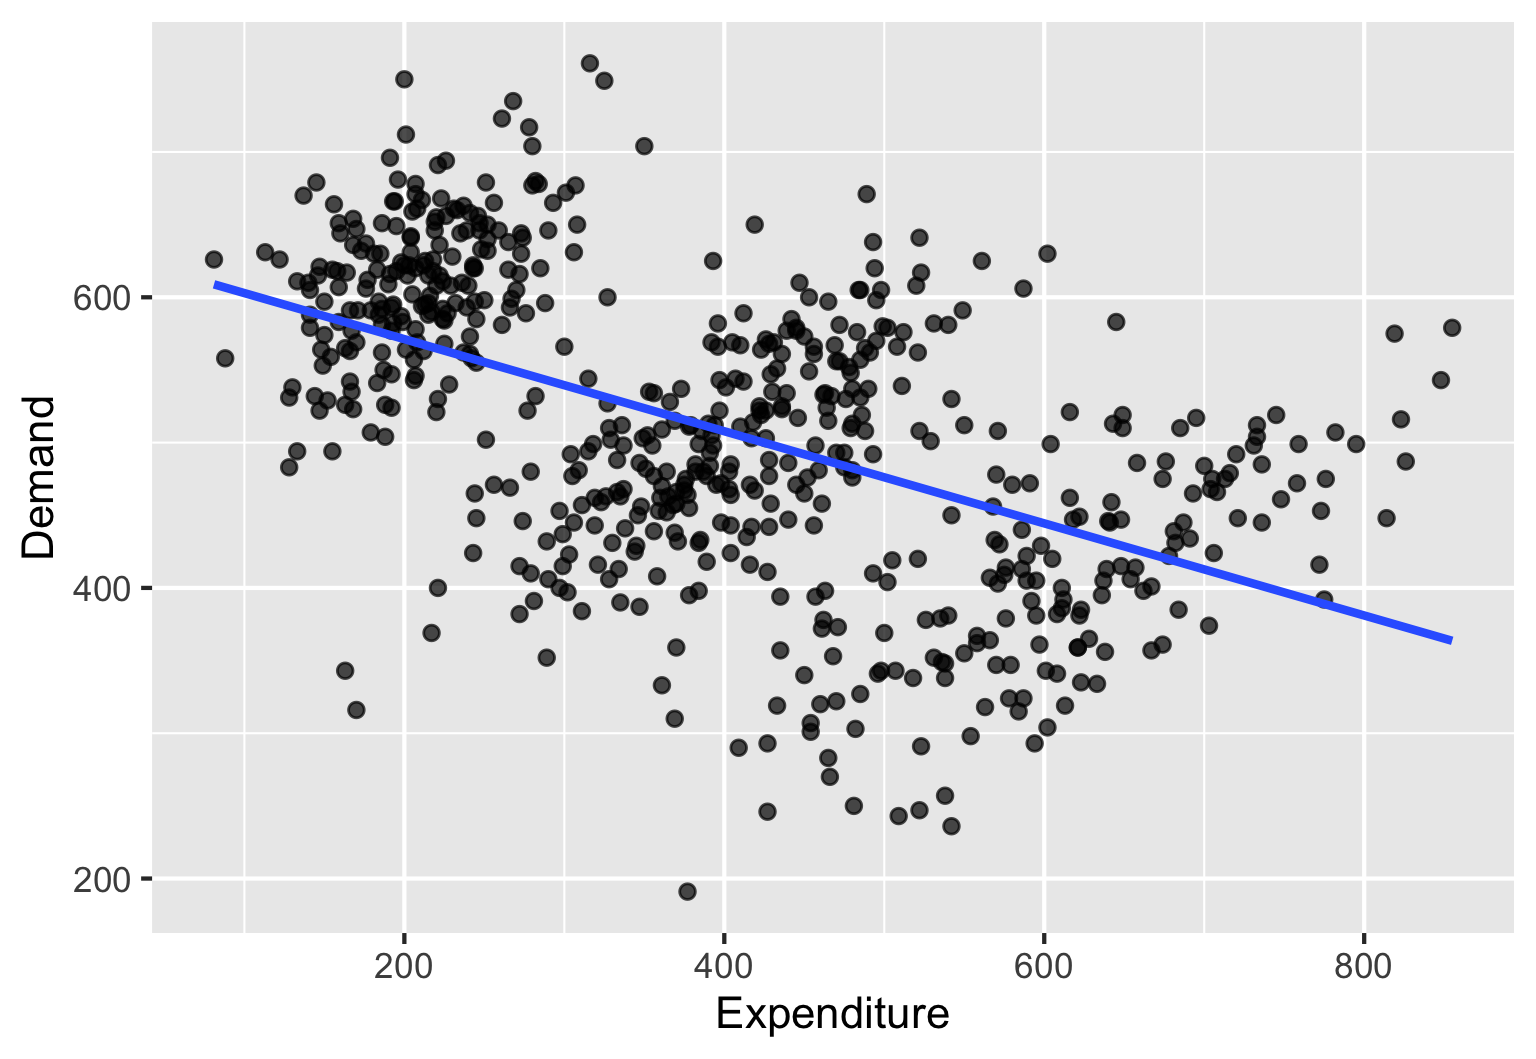
\includegraphics[width=0.7\linewidth,height=\textheight,keepaspectratio]{modules/05-explanatory-power-of-models/../../images/fig-simpson-overall.png}

}

\caption{\label{fig-simpson-overall}The curious relationship between
advertising expenditure and demand in the
\emph{demand\_expenditure\_simpson} data frame}

\end{figure}%

While the overall relationship is puzzling, we can see that the plot
itself shows three distinct clouds of points. This might lead us to
wonder if there is a variable we might be missing.

The data frame \emph{demand\_expenditure\_simpson} has a variable
\emph{Product}. Perhaps that has something to do with this
counter-intuitive finding.

Let us \emph{adjust} for product by including it in the model.

\begin{lstlisting}[language=R]
demand_expenditure_simpson |> 
  model_train(Demand ~ Expenditure + Product) |> 
  coef()
\end{lstlisting}

\begin{lstlisting}
(Intercept) Expenditure    ProductY    ProductZ 
    505.489       0.509    -207.555    -409.010 
\end{lstlisting}

We see now that the coefficient of \emph{Expenditure} is positive,
showing that higher expenditure is associated with higher demand. See
the model function in Equation~\ref{eq-simpson-adjusted}.

\begin{equation}\phantomsection\label{eq-simpson-adjusted}{
\widehat{Demand} = 505.5 + 0.51 \times Expenditure
\begin{cases}
+\,0 & \text{if } \text{Product} = \text{"ProductX"} \\
-\,207.6 & \text{if } \text{Product} = \text{"ProductY"} \\
-\,409 & \text{if } \text{Product} = \text{"ProductZ"}
\end{cases}
}\end{equation}

Plotting three separate regression lines for the three products confirms
this finding. See Figure~\ref{fig-simpson-adjusted}.

\begin{figure}

\centering{

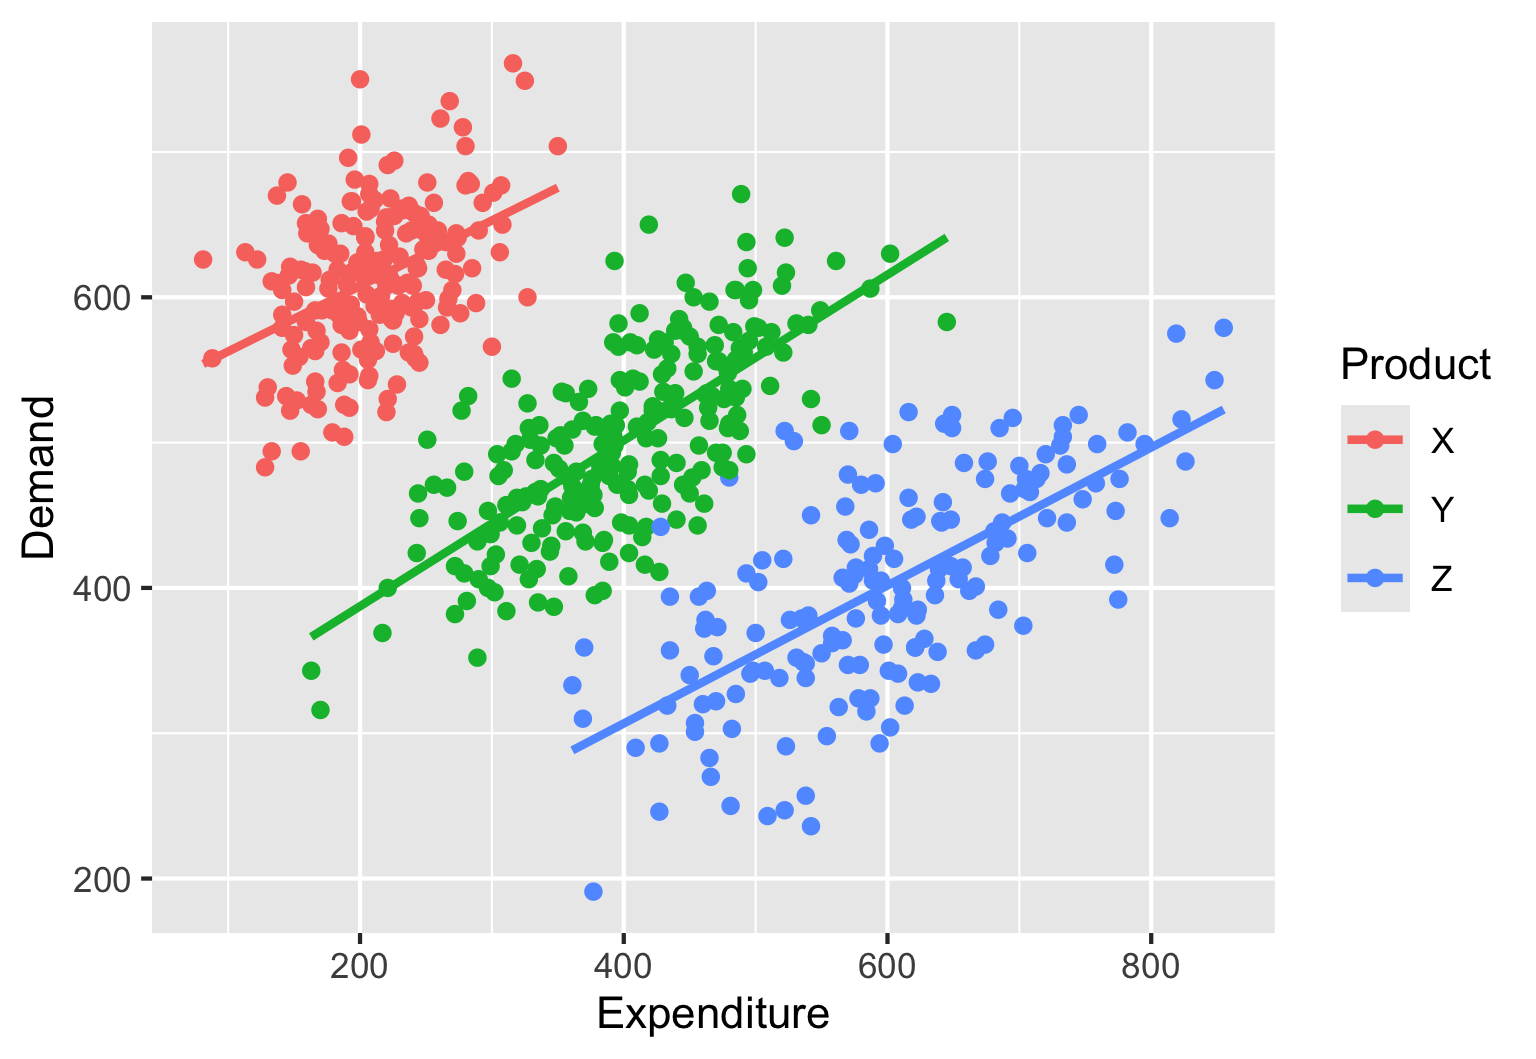
\includegraphics[width=0.7\linewidth,height=\textheight,keepaspectratio]{modules/05-explanatory-power-of-models/../../images/fig-simpson-adjusted.png}

}

\caption{\label{fig-simpson-adjusted}Relationships in the
\emph{demand\_expenditure\_simpson} data frame after adjusting for
\emph{product}}

\end{figure}%

\begin{tcolorbox}[enhanced jigsaw, colback=white, leftrule=.75mm, toprule=.15mm, bottomtitle=1mm, breakable, coltitle=black, toptitle=1mm, title={Quick Check}, opacitybacktitle=0.6, colbacktitle=quarto-callout-note-color!10!white, arc=.35mm, left=2mm, colframe=quarto-callout-note-color-frame, titlerule=0mm, rightrule=.15mm, bottomrule=.15mm, opacityback=0]

In the above example, why did the overall data give us an incorrect
picture of the effect of advertising on sales?

\end{tcolorbox}

\begin{tcolorbox}[enhanced jigsaw, colback=white, leftrule=.75mm, toprule=.15mm, bottomtitle=1mm, breakable, coltitle=black, toptitle=1mm, title={Suggested answer}, opacitybacktitle=0.6, colbacktitle=quarto-callout-note-color!10!white, arc=.35mm, left=2mm, colframe=quarto-callout-note-color-frame, titlerule=0mm, rightrule=.15mm, bottomrule=.15mm, opacityback=0]

The data for the three products were such that product Z had the highest
expenditures and the lowest demands, product Y had the next highest
expenditures and the next lowest demands, and product X had the lowest
expenditures and the highest demands. This created a situation where the
overall data showed a negative relationship between expenditure and
demand, even though within each product, there was a positive
relationship.

There was a systematic difference in the baseline demand for the three
products, and this created a situation where the overall relationship
was misleading. When we adjusted for product, we were able to see the
true positive relationship between expenditure and demand within each
product.

\end{tcolorbox}

\section{A word of caution about our
examples}\label{a-word-of-caution-about-our-examples}

We showed some dramatic examples to illustrate the importance of
adjustment. We do not mean to suggest that all comparisons of averages
or of relationships are misleading or will have sweeping effects when we
adjust for other variables.

However, we do want to stress that we should always be cautious and ask
ourselves if there are other variables that we need to adjust for before
accepting the story that the numbers are telling us.




\end{document}
